% Options for packages loaded elsewhere
\PassOptionsToPackage{unicode}{hyperref}
\PassOptionsToPackage{hyphens}{url}
%
\documentclass[
]{book}
\usepackage{amsmath,amssymb}
\usepackage{lmodern}
\usepackage{ifxetex,ifluatex}
\ifnum 0\ifxetex 1\fi\ifluatex 1\fi=0 % if pdftex
  \usepackage[T1]{fontenc}
  \usepackage[utf8]{inputenc}
  \usepackage{textcomp} % provide euro and other symbols
\else % if luatex or xetex
  \usepackage{unicode-math}
  \defaultfontfeatures{Scale=MatchLowercase}
  \defaultfontfeatures[\rmfamily]{Ligatures=TeX,Scale=1}
\fi
% Use upquote if available, for straight quotes in verbatim environments
\IfFileExists{upquote.sty}{\usepackage{upquote}}{}
\IfFileExists{microtype.sty}{% use microtype if available
  \usepackage[]{microtype}
  \UseMicrotypeSet[protrusion]{basicmath} % disable protrusion for tt fonts
}{}
\makeatletter
\@ifundefined{KOMAClassName}{% if non-KOMA class
  \IfFileExists{parskip.sty}{%
    \usepackage{parskip}
  }{% else
    \setlength{\parindent}{0pt}
    \setlength{\parskip}{6pt plus 2pt minus 1pt}}
}{% if KOMA class
  \KOMAoptions{parskip=half}}
\makeatother
\usepackage{xcolor}
\IfFileExists{xurl.sty}{\usepackage{xurl}}{} % add URL line breaks if available
\IfFileExists{bookmark.sty}{\usepackage{bookmark}}{\usepackage{hyperref}}
\hypersetup{
  pdftitle={R学习笔记},
  pdfauthor={Yufei Zhong},
  hidelinks,
  pdfcreator={LaTeX via pandoc}}
\urlstyle{same} % disable monospaced font for URLs
\usepackage{color}
\usepackage{fancyvrb}
\newcommand{\VerbBar}{|}
\newcommand{\VERB}{\Verb[commandchars=\\\{\}]}
\DefineVerbatimEnvironment{Highlighting}{Verbatim}{commandchars=\\\{\}}
% Add ',fontsize=\small' for more characters per line
\usepackage{framed}
\definecolor{shadecolor}{RGB}{248,248,248}
\newenvironment{Shaded}{\begin{snugshade}}{\end{snugshade}}
\newcommand{\AlertTok}[1]{\textcolor[rgb]{0.94,0.16,0.16}{#1}}
\newcommand{\AnnotationTok}[1]{\textcolor[rgb]{0.56,0.35,0.01}{\textbf{\textit{#1}}}}
\newcommand{\AttributeTok}[1]{\textcolor[rgb]{0.77,0.63,0.00}{#1}}
\newcommand{\BaseNTok}[1]{\textcolor[rgb]{0.00,0.00,0.81}{#1}}
\newcommand{\BuiltInTok}[1]{#1}
\newcommand{\CharTok}[1]{\textcolor[rgb]{0.31,0.60,0.02}{#1}}
\newcommand{\CommentTok}[1]{\textcolor[rgb]{0.56,0.35,0.01}{\textit{#1}}}
\newcommand{\CommentVarTok}[1]{\textcolor[rgb]{0.56,0.35,0.01}{\textbf{\textit{#1}}}}
\newcommand{\ConstantTok}[1]{\textcolor[rgb]{0.00,0.00,0.00}{#1}}
\newcommand{\ControlFlowTok}[1]{\textcolor[rgb]{0.13,0.29,0.53}{\textbf{#1}}}
\newcommand{\DataTypeTok}[1]{\textcolor[rgb]{0.13,0.29,0.53}{#1}}
\newcommand{\DecValTok}[1]{\textcolor[rgb]{0.00,0.00,0.81}{#1}}
\newcommand{\DocumentationTok}[1]{\textcolor[rgb]{0.56,0.35,0.01}{\textbf{\textit{#1}}}}
\newcommand{\ErrorTok}[1]{\textcolor[rgb]{0.64,0.00,0.00}{\textbf{#1}}}
\newcommand{\ExtensionTok}[1]{#1}
\newcommand{\FloatTok}[1]{\textcolor[rgb]{0.00,0.00,0.81}{#1}}
\newcommand{\FunctionTok}[1]{\textcolor[rgb]{0.00,0.00,0.00}{#1}}
\newcommand{\ImportTok}[1]{#1}
\newcommand{\InformationTok}[1]{\textcolor[rgb]{0.56,0.35,0.01}{\textbf{\textit{#1}}}}
\newcommand{\KeywordTok}[1]{\textcolor[rgb]{0.13,0.29,0.53}{\textbf{#1}}}
\newcommand{\NormalTok}[1]{#1}
\newcommand{\OperatorTok}[1]{\textcolor[rgb]{0.81,0.36,0.00}{\textbf{#1}}}
\newcommand{\OtherTok}[1]{\textcolor[rgb]{0.56,0.35,0.01}{#1}}
\newcommand{\PreprocessorTok}[1]{\textcolor[rgb]{0.56,0.35,0.01}{\textit{#1}}}
\newcommand{\RegionMarkerTok}[1]{#1}
\newcommand{\SpecialCharTok}[1]{\textcolor[rgb]{0.00,0.00,0.00}{#1}}
\newcommand{\SpecialStringTok}[1]{\textcolor[rgb]{0.31,0.60,0.02}{#1}}
\newcommand{\StringTok}[1]{\textcolor[rgb]{0.31,0.60,0.02}{#1}}
\newcommand{\VariableTok}[1]{\textcolor[rgb]{0.00,0.00,0.00}{#1}}
\newcommand{\VerbatimStringTok}[1]{\textcolor[rgb]{0.31,0.60,0.02}{#1}}
\newcommand{\WarningTok}[1]{\textcolor[rgb]{0.56,0.35,0.01}{\textbf{\textit{#1}}}}
\usepackage{longtable,booktabs,array}
\usepackage{calc} % for calculating minipage widths
% Correct order of tables after \paragraph or \subparagraph
\usepackage{etoolbox}
\makeatletter
\patchcmd\longtable{\par}{\if@noskipsec\mbox{}\fi\par}{}{}
\makeatother
% Allow footnotes in longtable head/foot
\IfFileExists{footnotehyper.sty}{\usepackage{footnotehyper}}{\usepackage{footnote}}
\makesavenoteenv{longtable}
\usepackage{graphicx}
\makeatletter
\def\maxwidth{\ifdim\Gin@nat@width>\linewidth\linewidth\else\Gin@nat@width\fi}
\def\maxheight{\ifdim\Gin@nat@height>\textheight\textheight\else\Gin@nat@height\fi}
\makeatother
% Scale images if necessary, so that they will not overflow the page
% margins by default, and it is still possible to overwrite the defaults
% using explicit options in \includegraphics[width, height, ...]{}
\setkeys{Gin}{width=\maxwidth,height=\maxheight,keepaspectratio}
% Set default figure placement to htbp
\makeatletter
\def\fps@figure{htbp}
\makeatother
\setlength{\emergencystretch}{3em} % prevent overfull lines
\providecommand{\tightlist}{%
  \setlength{\itemsep}{0pt}\setlength{\parskip}{0pt}}
\setcounter{secnumdepth}{5}
\usepackage{booktabs}
\ifluatex
  \usepackage{selnolig}  % disable illegal ligatures
\fi
\usepackage[]{natbib}
\bibliographystyle{apalike}

\title{R学习笔记}
\author{Yufei Zhong}
\date{2021-05-14}

\begin{document}
\maketitle

{
\setcounter{tocdepth}{1}
\tableofcontents
}
\hypertarget{ux8bf4ux660e}{%
\chapter{说明}\label{ux8bf4ux660e}}

作为商业数据分析师,我学习使用\texttt{R}已经有较长一段时间,主要用\texttt{R}来处理数据,自动化报表,ETL,可视化等;另外用R包\texttt{shiny}做web看板。

本文主要记录个人学习数据处理相关R包的过程,主要从\texttt{tidyverse}系列以及\texttt{data.table}两套语法做数据处理。co

\textbackslash begin\{center\}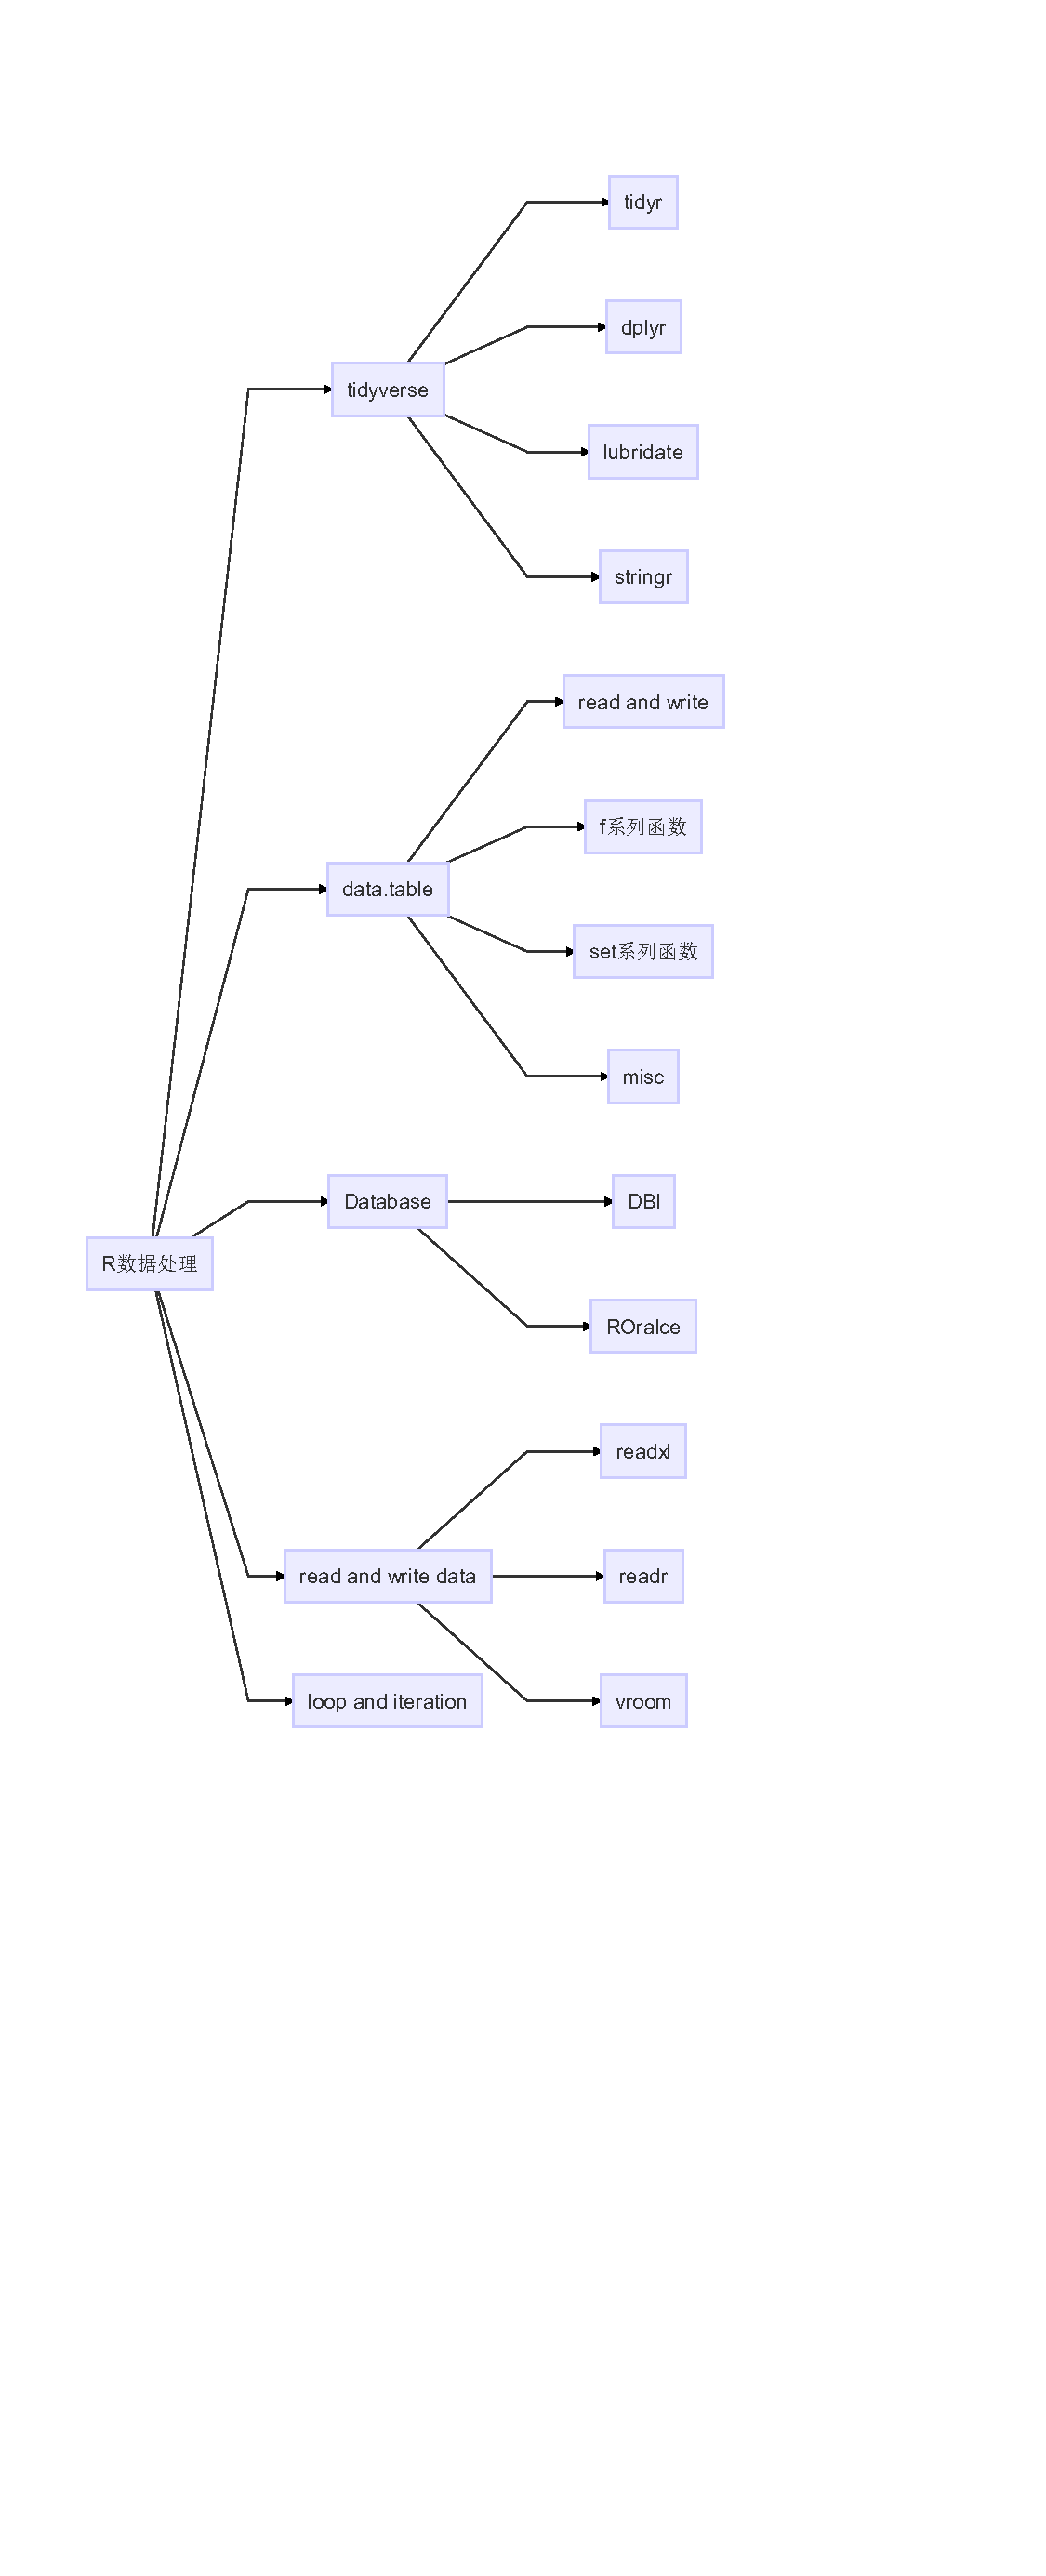
\includegraphics[width=0.7\linewidth]{Rbook_files/figure-latex/unnamed-chunk-3-1}

\texttt{R}极大的拓展了数据处理能力,让我很轻松方便处理数据,有更多精力时间聚焦在具体问题上。但因个人能力有限,难免出现错误,如阅读中发现错误,欢迎联系本人更正。

Email: \href{mailto:598253220@qq.com}{\nolinkurl{598253220@qq.com}}

微信公众号: 宇飞的世界

语雀: \url{https://www.yuque.com/zyufei}

\begin{Shaded}
\begin{Highlighting}[]
\CommentTok{\#查看版本信息}
\FunctionTok{sessionInfo}\NormalTok{()}
\CommentTok{\#\textgreater{} R version 4.0.5 (2021{-}03{-}31)}
\CommentTok{\#\textgreater{} Platform: x86\_64{-}w64{-}mingw32/x64 (64{-}bit)}
\CommentTok{\#\textgreater{} Running under: Windows 10 x64 (build 19041)}
\CommentTok{\#\textgreater{} }
\CommentTok{\#\textgreater{} Matrix products: default}
\CommentTok{\#\textgreater{} }
\CommentTok{\#\textgreater{} locale:}
\CommentTok{\#\textgreater{} [1] LC\_COLLATE=Chinese (Simplified)\_China.936 }
\CommentTok{\#\textgreater{} [2] LC\_CTYPE=Chinese (Simplified)\_China.936   }
\CommentTok{\#\textgreater{} [3] LC\_MONETARY=Chinese (Simplified)\_China.936}
\CommentTok{\#\textgreater{} [4] LC\_NUMERIC=C                              }
\CommentTok{\#\textgreater{} [5] LC\_TIME=Chinese (Simplified)\_China.936    }
\CommentTok{\#\textgreater{} }
\CommentTok{\#\textgreater{} attached base packages:}
\CommentTok{\#\textgreater{} [1] stats     graphics  grDevices utils     datasets  methods   base     }
\CommentTok{\#\textgreater{} }
\CommentTok{\#\textgreater{} other attached packages:}
\CommentTok{\#\textgreater{} [1] DiagrammeR\_1.0.6.1}
\CommentTok{\#\textgreater{} }
\CommentTok{\#\textgreater{} loaded via a namespace (and not attached):}
\CommentTok{\#\textgreater{}  [1] bookdown\_0.22      ps\_1.6.0           visNetwork\_2.0.9   digest\_0.6.27     }
\CommentTok{\#\textgreater{}  [5] R6\_2.5.0           jsonlite\_1.7.2     magrittr\_2.0.1     evaluate\_0.14     }
\CommentTok{\#\textgreater{}  [9] rlang\_0.4.11       stringi\_1.6.1      rstudioapi\_0.13    callr\_3.7.0       }
\CommentTok{\#\textgreater{} [13] rmarkdown\_2.8      webshot\_0.5.2      RColorBrewer\_1.1{-}2 tools\_4.0.5       }
\CommentTok{\#\textgreater{} [17] stringr\_1.4.0      htmlwidgets\_1.5.3  glue\_1.4.2         processx\_3.5.2    }
\CommentTok{\#\textgreater{} [21] xfun\_0.22          yaml\_2.2.1         compiler\_4.0.5     htmltools\_0.5.1.1 }
\CommentTok{\#\textgreater{} [25] knitr\_1.33}
\end{Highlighting}
\end{Shaded}

\hypertarget{ux8bfbux5199ux6570ux636e}{%
\chapter{读写数据}\label{ux8bfbux5199ux6570ux636e}}

在我们使用R做数据处理前,我们首先需要将数据从外界导入R中。但是现实生活中数据类型复杂,存在各种各样的数据文件。我们从连接方式简单区分为文本数据、数据库数据,也就是用文件存放的数据或在数据库中的数据。

关于和数据库的连接交互,请查看数据库章节。本章主要记录常用的Excel、csv、txt等文本文件的读写方式。

\hypertarget{readxl}{%
\section{readxl}\label{readxl}}

readxl软件包使R获取Excel数据变得简洁。与现有的软件包(例如:xlsx)相比,readxl没有外部依赖性。容易在所有的操作系统安装使用。

readxl\href{https://readxl.tidyverse.org/}{项目地址}。本节大部分代码来源项目官网介绍,可自行查阅官网。

\hypertarget{ux5b89ux88c5}{%
\subsection{安装}\label{ux5b89ux88c5}}

从CRAN安装最新发行版本的最简单方法是安装整个tidyverse。

\begin{Shaded}
\begin{Highlighting}[]
\FunctionTok{install.packages}\NormalTok{(}\StringTok{"tidyverse"}\NormalTok{)}
\end{Highlighting}
\end{Shaded}

\begin{quote}
由于readxl不是tidyverse核心加载包,使用时任需要加载library(readxl)
\end{quote}

或者是从CRAN仅安装readxl;

\begin{Shaded}
\begin{Highlighting}[]
\FunctionTok{install.packages}\NormalTok{(}\StringTok{"readxl"}\NormalTok{)}
\end{Highlighting}
\end{Shaded}

从github安装开发版:

\begin{Shaded}
\begin{Highlighting}[]
\CommentTok{\# install.packages("devtools")}
\NormalTok{devtools}\SpecialCharTok{::}\FunctionTok{install\_github}\NormalTok{(}\StringTok{"tidyverse/readxl"}\NormalTok{)}
\end{Highlighting}
\end{Shaded}

\hypertarget{ux7528ux6cd5}{%
\subsection{用法}\label{ux7528ux6cd5}}

1.读取

readxl包中包含了几个示例文件,我们在接下来的案例中使用。

\begin{itemize}
\tightlist
\item
  查看readxl包中自带xlsx文件
\end{itemize}

\begin{Shaded}
\begin{Highlighting}[]
\FunctionTok{library}\NormalTok{(readxl)}
\FunctionTok{readxl\_example}\NormalTok{()}
\FunctionTok{readxl\_example}\NormalTok{(}\StringTok{"clippy.xls"}\NormalTok{)}
\end{Highlighting}
\end{Shaded}

\texttt{read\_excel()}可读取xls和xlsx文件。

\begin{Shaded}
\begin{Highlighting}[]
\NormalTok{xlsx\_example }\OtherTok{\textless{}{-}} \FunctionTok{readxl\_example}\NormalTok{(}\StringTok{"datasets.xlsx"}\NormalTok{)}
\FunctionTok{read\_excel}\NormalTok{(xlsx\_example)}
\end{Highlighting}
\end{Shaded}

通过函数\texttt{excel\_sheets()}查看Excel的sheet名称

\begin{Shaded}
\begin{Highlighting}[]
\FunctionTok{excel\_sheets}\NormalTok{(xlsx\_example)}
\end{Highlighting}
\end{Shaded}

指定worksheet的名字读取,可以是sheet的名字或序号。

当我们要读取的本地xlsx文件有多个sheets时,通过值定sheet参数读取指定的sheet。

\begin{Shaded}
\begin{Highlighting}[]
\FunctionTok{read\_excel}\NormalTok{(xlsx\_example, }\AttributeTok{sheet =} \StringTok{"chickwts"}\NormalTok{)}
\end{Highlighting}
\end{Shaded}

读取xlsx文件的指定位置,有多种方法控制。本处提供几个案例,请\texttt{?read\_excel()}查看帮助。

\begin{Shaded}
\begin{Highlighting}[]
\FunctionTok{read\_excel}\NormalTok{(path, }\AttributeTok{sheet =} \ConstantTok{NULL}\NormalTok{, }\AttributeTok{range =} \ConstantTok{NULL}\NormalTok{, }\AttributeTok{col\_names =} \ConstantTok{TRUE}\NormalTok{,}
  \AttributeTok{col\_types =} \ConstantTok{NULL}\NormalTok{, }\AttributeTok{na =} \StringTok{""}\NormalTok{, }\AttributeTok{trim\_ws =} \ConstantTok{TRUE}\NormalTok{, }\AttributeTok{skip =} \DecValTok{0}\NormalTok{,}
  \AttributeTok{n\_max =} \ConstantTok{Inf}\NormalTok{, }\AttributeTok{guess\_max =} \FunctionTok{min}\NormalTok{(}\DecValTok{1000}\NormalTok{, n\_max),}
  \AttributeTok{progress =} \FunctionTok{readxl\_progress}\NormalTok{(), }\AttributeTok{.name\_repair =} \StringTok{"unique"}\NormalTok{)}
\end{Highlighting}
\end{Shaded}

range接受单元格范围,最简单的表示方式即Excle中单元格表示方法,如as range = ``D12:F15'' or range = ``R1C12:R6C15''.

其余参数中,个人觉得col\_types比较重要,可以指定列的类型。可用选项:``skip'', ``guess'', ``logical'', ``numeric'', ``date'', ``text'' or ``list''。

\hypertarget{writexl}{%
\section{writexl}\label{writexl}}

writexl包目前的功能比较简单,仅有读写Excel功能,但优势是速度较快,尤其是写入Excel时。\href{https://docs.ropensci.org/writexl/}{项目地址}

\hypertarget{ux7528ux6cd5-1}{%
\subsection{用法}\label{ux7528ux6cd5-1}}

安装

\begin{Shaded}
\begin{Highlighting}[]
\FunctionTok{install.packages}\NormalTok{(}\StringTok{"writexl"}\NormalTok{)}
\end{Highlighting}
\end{Shaded}

参数

\begin{Shaded}
\begin{Highlighting}[]
\FunctionTok{write\_xlsx}\NormalTok{(}
\NormalTok{  x,}
  \AttributeTok{path =} \FunctionTok{tempfile}\NormalTok{(}\AttributeTok{fileext =} \StringTok{".xlsx"}\NormalTok{),}
  \AttributeTok{col\_names =} \ConstantTok{TRUE}\NormalTok{,}
  \AttributeTok{format\_headers =} \ConstantTok{TRUE}\NormalTok{,}
  \AttributeTok{use\_zip64 =} \ConstantTok{FALSE}
\NormalTok{)}
\end{Highlighting}
\end{Shaded}

输出Excel

\begin{Shaded}
\begin{Highlighting}[]
\FunctionTok{library}\NormalTok{(writexl)}
\NormalTok{writexl}\SpecialCharTok{::}\FunctionTok{write\_xlsx}\NormalTok{(iris,}\AttributeTok{path =} \StringTok{\textquotesingle{}iris.xlsx\textquotesingle{}}\NormalTok{)}
\FunctionTok{write\_xlsx}\NormalTok{(}\FunctionTok{list}\NormalTok{(}\AttributeTok{mysheet1 =}\NormalTok{ iris,}\AttributeTok{mysheet2 =}\NormalTok{ iris),}\AttributeTok{path =} \StringTok{\textquotesingle{}iris.xlsx\textquotesingle{}}\NormalTok{)}
\end{Highlighting}
\end{Shaded}

效率比较

\begin{Shaded}
\begin{Highlighting}[]
\FunctionTok{library}\NormalTok{(microbenchmark)}
\FunctionTok{library}\NormalTok{(nycflights13)}
\FunctionTok{microbenchmark}\NormalTok{(}
  \AttributeTok{writexl =}\NormalTok{ writexl}\SpecialCharTok{::}\FunctionTok{write\_xlsx}\NormalTok{(flights, }\FunctionTok{tempfile}\NormalTok{()),}
  \AttributeTok{openxlsx =}\NormalTok{ openxlsx}\SpecialCharTok{::}\FunctionTok{write.xlsx}\NormalTok{(flights, }\FunctionTok{tempfile}\NormalTok{()),}
  \AttributeTok{times =} \DecValTok{2}
\NormalTok{)}
\end{Highlighting}
\end{Shaded}

其它功能

\begin{Shaded}
\begin{Highlighting}[]
\NormalTok{df }\OtherTok{\textless{}{-}} \FunctionTok{data.frame}\NormalTok{(}
  \AttributeTok{name =} \FunctionTok{c}\NormalTok{(}\StringTok{"UCLA"}\NormalTok{, }\StringTok{"Berkeley"}\NormalTok{, }\StringTok{"Jeroen"}\NormalTok{),}
  \AttributeTok{founded =} \FunctionTok{c}\NormalTok{(}\DecValTok{1919}\NormalTok{, }\DecValTok{1868}\NormalTok{, }\DecValTok{2030}\NormalTok{),}
  \AttributeTok{website =} \FunctionTok{xl\_hyperlink}\NormalTok{(}\FunctionTok{c}\NormalTok{(}\StringTok{"http://www.ucla.edu"}\NormalTok{, }\StringTok{"http://www.berkeley.edu"}\NormalTok{, }\ConstantTok{NA}\NormalTok{), }\StringTok{"homepage"}\NormalTok{)}
\NormalTok{)}
\NormalTok{df}\SpecialCharTok{$}\NormalTok{age }\OtherTok{\textless{}{-}} \FunctionTok{xl\_formula}\NormalTok{(}\StringTok{\textquotesingle{}=(YEAR(TODAY()) {-} INDIRECT("B" \& ROW()))\textquotesingle{}}\NormalTok{)}
\FunctionTok{write\_xlsx}\NormalTok{(df, }\StringTok{\textquotesingle{}universities.xlsx\textquotesingle{}}\NormalTok{)}

\CommentTok{\# cleanup}
\FunctionTok{unlink}\NormalTok{(}\StringTok{\textquotesingle{}universities.xlsx\textquotesingle{}}\NormalTok{)}
\end{Highlighting}
\end{Shaded}

\hypertarget{openxlsx}{%
\section{openxlsx}\label{openxlsx}}

openxlsx是当我需要定制输出Excel表格或报表时常用R包。目前该包的版本4.2.3,通过使用Rcpp加速,包的读写速度在Excel的百万级下是可接受状态,包的相关函数功能完善且简易好用,并且正在积极开发中,相信它以后功能会越来越强大。

项目官方地址:\url{https://ycphs.github.io/openxlsx/index.html}

个人感觉主要优势:

\begin{itemize}
\tightlist
\item
  不依赖java环境
\item
  读写速度可接受
\item
  可设置条件格式,与Excel中『开始』选项卡的条件格式功能接近
\item
  可批量插入ggplot2图
\item
  可插入公式
\item
  可渲染大部分Excel格式,并且效率相比部分python包高效
\item
  可添加页眉页脚以及其他格式,方便直接打印
\item
  功能稳定可用并且在积极开发中
\end{itemize}

版本信息查看

\begin{Shaded}
\begin{Highlighting}[]
\FunctionTok{packageVersion}\NormalTok{(}\StringTok{"openxlsx"}\NormalTok{)}
\end{Highlighting}
\end{Shaded}

本人公众号:宇飞的世界中有更加详细的阐述:\url{https://mp.weixin.qq.com/s/ZD0dJb0y8fsWGI1dCPh2mQ}

\hypertarget{ux5b89ux88c5-1}{%
\subsection{安装}\label{ux5b89ux88c5-1}}

稳定版

\begin{Shaded}
\begin{Highlighting}[]
\CommentTok{\# 稳定版}
\FunctionTok{install.packages}\NormalTok{(}\StringTok{"openxlsx"}\NormalTok{, }\AttributeTok{dependencies =} \ConstantTok{TRUE}\NormalTok{, }\AttributeTok{repos =} \StringTok{"https://mirrors.tuna.tsinghua.edu.cn/CRAN/"}\NormalTok{)}
\end{Highlighting}
\end{Shaded}

开发版

\begin{Shaded}
\begin{Highlighting}[]
\FunctionTok{install.packages}\NormalTok{(}\FunctionTok{c}\NormalTok{(}\StringTok{"Rcpp"}\NormalTok{, }\StringTok{"devtools"}\NormalTok{), }\AttributeTok{dependencies =} \ConstantTok{TRUE}\NormalTok{)}
\FunctionTok{library}\NormalTok{(devtools)}
\FunctionTok{install\_github}\NormalTok{(}\StringTok{"ycphs/openxlsx"}\NormalTok{)}
\end{Highlighting}
\end{Shaded}

\hypertarget{ux57faux7840ux529fux80fd}{%
\subsection{基础功能}\label{ux57faux7840ux529fux80fd}}

本文仅呈现基础功能部分,即读写EXCEL文件。其它功能,请查阅项目官方地址或微信公众号文章\href{https://mp.weixin.qq.com/s/ZD0dJb0y8fsWGI1dCPh2mQ}{R包-openxlsx-学习笔记}

\hypertarget{ux8bfbux53d6excel}{%
\subsubsection{读取Excel}\label{ux8bfbux53d6excel}}

read.xlsx()是读取函数,主要参数如下:

\begin{Shaded}
\begin{Highlighting}[]
\FunctionTok{library}\NormalTok{(openxlsx)}
\FunctionTok{read.xlsx}\NormalTok{(}
\NormalTok{  xlsxFile,}
  \AttributeTok{sheet =} \DecValTok{1}\NormalTok{,}
  \AttributeTok{startRow =} \DecValTok{1}\NormalTok{,}
  \AttributeTok{colNames =} \ConstantTok{TRUE}\NormalTok{,}
  \AttributeTok{rowNames =} \ConstantTok{FALSE}\NormalTok{,}
  \AttributeTok{detectDates =} \ConstantTok{FALSE}\NormalTok{,}
  \AttributeTok{skipEmptyRows =} \ConstantTok{TRUE}\NormalTok{,}
  \AttributeTok{skipEmptyCols =} \ConstantTok{TRUE}\NormalTok{,}
  \AttributeTok{rows =} \ConstantTok{NULL}\NormalTok{,}
  \AttributeTok{cols =} \ConstantTok{NULL}\NormalTok{,}
  \AttributeTok{check.names =} \ConstantTok{FALSE}\NormalTok{,}
  \AttributeTok{sep.names =} \StringTok{"."}\NormalTok{,}
  \AttributeTok{namedRegion =} \ConstantTok{NULL}\NormalTok{,}
  \AttributeTok{na.strings =} \StringTok{"NA"}\NormalTok{,}
  \AttributeTok{fillMergedCells =} \ConstantTok{FALSE}
\NormalTok{)}
\end{Highlighting}
\end{Shaded}

以上参数中需要注意 :

detecDates参数,当你的Excel表格中带日期列时需要将参数设置为TRUE,不然将会把日期识别为数字读入。

fillMergedCells参数,当你读取的表格中存在合并单元格,将用值填充其他全部单元格,如下所示:

\includegraphics{https://gitee.com/zhongyufei/photo-bed/raw/pic/img/merge-cell-xlsx.png}

\begin{Shaded}
\begin{Highlighting}[]
\FunctionTok{read.xlsx}\NormalTok{(}\StringTok{\textquotesingle{}./test.xlsx\textquotesingle{}}\NormalTok{,}\AttributeTok{detectDates =} \ConstantTok{TRUE}\NormalTok{,}\AttributeTok{fillMergedCells =} \ConstantTok{TRUE}\NormalTok{)}
\end{Highlighting}
\end{Shaded}

读取后如下所示:

\begin{figure}
\centering
\includegraphics{https://gitee.com/zhongyufei/photo-bed/raw/pic/img/R-read-merge-xlsx.png}
\caption{openxlsx-merge-xlsx}
\end{figure}

readWorkbook()也可以读取Excel表格数据,参数与read.xlsx基本一致。

\begin{Shaded}
\begin{Highlighting}[]
\NormalTok{xlsxFile }\OtherTok{\textless{}{-}} \FunctionTok{system.file}\NormalTok{(}\StringTok{"extdata"}\NormalTok{, }\StringTok{"readTest.xlsx"}\NormalTok{, }\AttributeTok{package =} \StringTok{"openxlsx"}\NormalTok{)}
\NormalTok{df1 }\OtherTok{\textless{}{-}} \FunctionTok{readWorkbook}\NormalTok{(}\AttributeTok{xlsxFile =}\NormalTok{ xlsxFile, }\AttributeTok{sheet =} \DecValTok{1}\NormalTok{)}
\end{Highlighting}
\end{Shaded}

\hypertarget{ux5199ux5165excel}{%
\subsubsection{写入Excel}\label{ux5199ux5165excel}}

我们将R中的数据有时候需要导出到Excle中,这时就利用函数将data.frame写入Excle。

write.xlsx()函数写入

\begin{Shaded}
\begin{Highlighting}[]
\FunctionTok{write.xlsx}\NormalTok{(iris, }\AttributeTok{file =} \StringTok{"writeXLSX1.xlsx"}\NormalTok{, }\AttributeTok{colNames =} \ConstantTok{TRUE}\NormalTok{, }\AttributeTok{borders =} \StringTok{"columns"}\NormalTok{)}
\end{Highlighting}
\end{Shaded}

带格式输出

\begin{Shaded}
\begin{Highlighting}[]
\NormalTok{hs }\OtherTok{\textless{}{-}} \FunctionTok{createStyle}\NormalTok{(}
  \AttributeTok{textDecoration =} \StringTok{"BOLD"}\NormalTok{, }\AttributeTok{fontColour =} \StringTok{"\#FFFFFF"}\NormalTok{, }\AttributeTok{fontSize =} \DecValTok{12}\NormalTok{,}
  \AttributeTok{fontName =} \StringTok{"Arial Narrow"}\NormalTok{, }\AttributeTok{fgFill =} \StringTok{"\#4F80BD"}
\NormalTok{)}
\DocumentationTok{\#\# Not run: }
\FunctionTok{write.xlsx}\NormalTok{(iris,}
  \AttributeTok{file =} \StringTok{"writeXLSX3.xlsx"}\NormalTok{,}
  \AttributeTok{colNames =} \ConstantTok{TRUE}\NormalTok{, }\AttributeTok{borders =} \StringTok{"rows"}\NormalTok{, }\AttributeTok{headerStyle =}\NormalTok{ hs}
\NormalTok{)}
\end{Highlighting}
\end{Shaded}

或者是用如下方式写入:

不带任何格式写入,共计四步。第一步创建workbook,第二步添加sheet,第三步写入数据,第四步保存workbook。

\begin{Shaded}
\begin{Highlighting}[]
\NormalTok{df }\OtherTok{\textless{}{-}} \FunctionTok{data.frame}\NormalTok{(}\AttributeTok{a=}\DecValTok{1}\SpecialCharTok{:}\DecValTok{10}\NormalTok{,}\AttributeTok{b=}\DecValTok{1}\SpecialCharTok{:}\DecValTok{10}\NormalTok{,}\AttributeTok{d=}\DecValTok{1}\SpecialCharTok{:}\DecValTok{10}\NormalTok{)}
\NormalTok{wb }\OtherTok{\textless{}{-}} \FunctionTok{createWorkbook}\NormalTok{(}\AttributeTok{creator =} \StringTok{\textquotesingle{}zhongyf\textquotesingle{}}\NormalTok{,}\AttributeTok{title =} \StringTok{\textquotesingle{}test\textquotesingle{}}\NormalTok{)}
\FunctionTok{addWorksheet}\NormalTok{(wb,}\AttributeTok{sheetName =} \StringTok{\textquotesingle{}test\textquotesingle{}}\NormalTok{)}
\FunctionTok{writeData}\NormalTok{(wb,}\AttributeTok{sheet =} \StringTok{\textquotesingle{}test\textquotesingle{}}\NormalTok{,}\AttributeTok{x =}\NormalTok{ df)}
\FunctionTok{saveWorkbook}\NormalTok{(wb, }\StringTok{"test.xlsx"}\NormalTok{, }\AttributeTok{overwrite =} \ConstantTok{TRUE}\NormalTok{)}
\end{Highlighting}
\end{Shaded}

\hypertarget{ux5e26ux683cux5f0fux8f93ux51fa}{%
\subsection{带格式输出}\label{ux5e26ux683cux5f0fux8f93ux51fa}}

我们以上面四步输出的方式举例,拆解其中四个函数的参数。

\begin{itemize}
\item
  createWorkbook()
\item
  addWorksheet()
\item
  writeData()
\item
  saveWorkbook()
\end{itemize}

首先看看包中自带的例子,我们分解其中的参数。

\begin{Shaded}
\begin{Highlighting}[]
\NormalTok{wb }\OtherTok{\textless{}{-}} \FunctionTok{createWorkbook}\NormalTok{(}\StringTok{"Fred"}\NormalTok{)}

\DocumentationTok{\#\# Add 3 worksheets}
\FunctionTok{addWorksheet}\NormalTok{(wb, }\StringTok{"Sheet 1"}\NormalTok{)}
\FunctionTok{addWorksheet}\NormalTok{(wb, }\StringTok{"Sheet 2"}\NormalTok{, }\AttributeTok{gridLines =} \ConstantTok{FALSE}\NormalTok{)}
\FunctionTok{addWorksheet}\NormalTok{(wb, }\StringTok{"Sheet 3"}\NormalTok{, }\AttributeTok{tabColour =} \StringTok{"red"}\NormalTok{)}
\FunctionTok{addWorksheet}\NormalTok{(wb, }\StringTok{"Sheet 4"}\NormalTok{, }\AttributeTok{gridLines =} \ConstantTok{FALSE}\NormalTok{, }\AttributeTok{tabColour =} \StringTok{"\#4F81BD"}\NormalTok{)}

\DocumentationTok{\#\# Headers and Footers}
\FunctionTok{addWorksheet}\NormalTok{(wb, }\StringTok{"Sheet 5"}\NormalTok{,}
  \AttributeTok{header =} \FunctionTok{c}\NormalTok{(}\StringTok{"ODD HEAD LEFT"}\NormalTok{, }\StringTok{"ODD HEAD CENTER"}\NormalTok{, }\StringTok{"ODD HEAD RIGHT"}\NormalTok{),}
  \AttributeTok{footer =} \FunctionTok{c}\NormalTok{(}\StringTok{"ODD FOOT RIGHT"}\NormalTok{, }\StringTok{"ODD FOOT CENTER"}\NormalTok{, }\StringTok{"ODD FOOT RIGHT"}\NormalTok{),}
  \AttributeTok{evenHeader =} \FunctionTok{c}\NormalTok{(}\StringTok{"EVEN HEAD LEFT"}\NormalTok{, }\StringTok{"EVEN HEAD CENTER"}\NormalTok{, }\StringTok{"EVEN HEAD RIGHT"}\NormalTok{),}
  \AttributeTok{evenFooter =} \FunctionTok{c}\NormalTok{(}\StringTok{"EVEN FOOT RIGHT"}\NormalTok{, }\StringTok{"EVEN FOOT CENTER"}\NormalTok{, }\StringTok{"EVEN FOOT RIGHT"}\NormalTok{),}
  \AttributeTok{firstHeader =} \FunctionTok{c}\NormalTok{(}\StringTok{"TOP"}\NormalTok{, }\StringTok{"OF FIRST"}\NormalTok{, }\StringTok{"PAGE"}\NormalTok{),}
  \AttributeTok{firstFooter =} \FunctionTok{c}\NormalTok{(}\StringTok{"BOTTOM"}\NormalTok{, }\StringTok{"OF FIRST"}\NormalTok{, }\StringTok{"PAGE"}\NormalTok{)}
\NormalTok{)}

\FunctionTok{addWorksheet}\NormalTok{(wb, }\StringTok{"Sheet 6"}\NormalTok{,}
  \AttributeTok{header =} \FunctionTok{c}\NormalTok{(}\StringTok{"\&[Date]"}\NormalTok{, }\StringTok{"ALL HEAD CENTER 2"}\NormalTok{, }\StringTok{"\&[Page] / \&[Pages]"}\NormalTok{),}
  \AttributeTok{footer =} \FunctionTok{c}\NormalTok{(}\StringTok{"\&[Path]\&[File]"}\NormalTok{, }\ConstantTok{NA}\NormalTok{, }\StringTok{"\&[Tab]"}\NormalTok{),}
  \AttributeTok{firstHeader =} \FunctionTok{c}\NormalTok{(}\ConstantTok{NA}\NormalTok{, }\StringTok{"Center Header of First Page"}\NormalTok{, }\ConstantTok{NA}\NormalTok{),}
  \AttributeTok{firstFooter =} \FunctionTok{c}\NormalTok{(}\ConstantTok{NA}\NormalTok{, }\StringTok{"Center Footer of First Page"}\NormalTok{, }\ConstantTok{NA}\NormalTok{)}
\NormalTok{)}

\FunctionTok{addWorksheet}\NormalTok{(wb, }\StringTok{"Sheet 7"}\NormalTok{,}
  \AttributeTok{header =} \FunctionTok{c}\NormalTok{(}\StringTok{"ALL HEAD LEFT 2"}\NormalTok{, }\StringTok{"ALL HEAD CENTER 2"}\NormalTok{, }\StringTok{"ALL HEAD RIGHT 2"}\NormalTok{),}
  \AttributeTok{footer =} \FunctionTok{c}\NormalTok{(}\StringTok{"ALL FOOT RIGHT 2"}\NormalTok{, }\StringTok{"ALL FOOT CENTER 2"}\NormalTok{, }\StringTok{"ALL FOOT RIGHT 2"}\NormalTok{)}
\NormalTok{)}

\FunctionTok{addWorksheet}\NormalTok{(wb, }\StringTok{"Sheet 8"}\NormalTok{,}
  \AttributeTok{firstHeader =} \FunctionTok{c}\NormalTok{(}\StringTok{"FIRST ONLY L"}\NormalTok{, }\ConstantTok{NA}\NormalTok{, }\StringTok{"FIRST ONLY R"}\NormalTok{),}
  \AttributeTok{firstFooter =} \FunctionTok{c}\NormalTok{(}\StringTok{"FIRST ONLY L"}\NormalTok{, }\ConstantTok{NA}\NormalTok{, }\StringTok{"FIRST ONLY R"}\NormalTok{)}
\NormalTok{)}

\DocumentationTok{\#\# Need data on worksheet to see all headers and footers}
\FunctionTok{writeData}\NormalTok{(wb, }\AttributeTok{sheet =} \DecValTok{5}\NormalTok{, }\DecValTok{1}\SpecialCharTok{:}\DecValTok{400}\NormalTok{)}
\FunctionTok{writeData}\NormalTok{(wb, }\AttributeTok{sheet =} \DecValTok{6}\NormalTok{, }\DecValTok{1}\SpecialCharTok{:}\DecValTok{400}\NormalTok{)}
\FunctionTok{writeData}\NormalTok{(wb, }\AttributeTok{sheet =} \DecValTok{7}\NormalTok{, }\DecValTok{1}\SpecialCharTok{:}\DecValTok{400}\NormalTok{)}
\FunctionTok{writeData}\NormalTok{(wb, }\AttributeTok{sheet =} \DecValTok{8}\NormalTok{, }\DecValTok{1}\SpecialCharTok{:}\DecValTok{400}\NormalTok{)}

\DocumentationTok{\#\# Save workbook}
\DocumentationTok{\#\# Not run: }
\FunctionTok{saveWorkbook}\NormalTok{(wb, }\StringTok{"addWorksheetExample.xlsx"}\NormalTok{, }\AttributeTok{overwrite =} \ConstantTok{TRUE}\NormalTok{)}
\end{Highlighting}
\end{Shaded}

\hypertarget{ux57faux7840ux51fdux6570}{%
\subsection{基础函数}\label{ux57faux7840ux51fdux6570}}

输出Excel的四步。\texttt{createWorkbook},\texttt{addWorksheet},\texttt{writeDataTable},\texttt{saveWorkbook}四个函数的参数解释。

\begin{itemize}
\tightlist
\item
  createWorkbook
\end{itemize}

\begin{Shaded}
\begin{Highlighting}[]
\FunctionTok{createWorkbook}\NormalTok{(}
  \AttributeTok{creator =} \FunctionTok{ifelse}\NormalTok{(.Platform}\SpecialCharTok{$}\NormalTok{OS.type }\SpecialCharTok{==} \StringTok{"windows"}\NormalTok{, }\FunctionTok{Sys.getenv}\NormalTok{(}\StringTok{"USERNAME"}\NormalTok{),}
    \FunctionTok{Sys.getenv}\NormalTok{(}\StringTok{"USER"}\NormalTok{)),}
  \AttributeTok{title =} \ConstantTok{NULL}\NormalTok{,}
  \AttributeTok{subject =} \ConstantTok{NULL}\NormalTok{,}
  \AttributeTok{category =} \ConstantTok{NULL}
\NormalTok{)}
\end{Highlighting}
\end{Shaded}

\begin{Shaded}
\begin{Highlighting}[]
\NormalTok{wb }\OtherTok{\textless{}{-}} \FunctionTok{createWorkbook}\NormalTok{(}
  \AttributeTok{creator =} \StringTok{"宇飞的世界"}\NormalTok{,}
  \AttributeTok{title =} \StringTok{"标题"}\NormalTok{,}
  \AttributeTok{subject =} \StringTok{"主题"}\NormalTok{,}
  \AttributeTok{category =} \StringTok{"类别目录"}
\NormalTok{)}
\end{Highlighting}
\end{Shaded}

\begin{itemize}
\tightlist
\item
  addWorksheet
\end{itemize}

\begin{Shaded}
\begin{Highlighting}[]
\FunctionTok{addWorksheet}\NormalTok{(}
\NormalTok{  wb,}
\NormalTok{  sheetName,}
  \AttributeTok{gridLines =} \ConstantTok{TRUE}\NormalTok{,}
  \AttributeTok{tabColour =} \ConstantTok{NULL}\NormalTok{,}
  \AttributeTok{zoom =} \DecValTok{100}\NormalTok{,}
  \AttributeTok{header =} \ConstantTok{NULL}\NormalTok{,}
  \AttributeTok{footer =} \ConstantTok{NULL}\NormalTok{,}
  \AttributeTok{evenHeader =} \ConstantTok{NULL}\NormalTok{,}
  \AttributeTok{evenFooter =} \ConstantTok{NULL}\NormalTok{,}
  \AttributeTok{firstHeader =} \ConstantTok{NULL}\NormalTok{,}
  \AttributeTok{firstFooter =} \ConstantTok{NULL}\NormalTok{,}
  \AttributeTok{visible =} \ConstantTok{TRUE}\NormalTok{,}
  \AttributeTok{paperSize =} \FunctionTok{getOption}\NormalTok{(}\StringTok{"openxlsx.paperSize"}\NormalTok{, }\AttributeTok{default =} \DecValTok{9}\NormalTok{),}
  \AttributeTok{orientation =} \FunctionTok{getOption}\NormalTok{(}\StringTok{"openxlsx.orientation"}\NormalTok{, }\AttributeTok{default =} \StringTok{"portrait"}\NormalTok{),}
  \AttributeTok{vdpi =} \FunctionTok{getOption}\NormalTok{(}\StringTok{"openxlsx.vdpi"}\NormalTok{, }\AttributeTok{default =} \FunctionTok{getOption}\NormalTok{(}\StringTok{"openxlsx.dpi"}\NormalTok{, }\AttributeTok{default =} \DecValTok{300}\NormalTok{)),}
  \AttributeTok{hdpi =} \FunctionTok{getOption}\NormalTok{(}\StringTok{"openxlsx.hdpi"}\NormalTok{, }\AttributeTok{default =} \FunctionTok{getOption}\NormalTok{(}\StringTok{"openxlsx.dpi"}\NormalTok{, }\AttributeTok{default =} \DecValTok{300}\NormalTok{))}
\NormalTok{)}
\end{Highlighting}
\end{Shaded}

\begin{Shaded}
\begin{Highlighting}[]
\NormalTok{gridLines参数:表格中是否有网格线,在Excle『视图』选项卡下面的网格线去除打勾的效果一致}

\NormalTok{tabColour参数:输出表格sheet标签颜色}

\NormalTok{zoom:发大缩小,默认是100,可选范围10}\DecValTok{{-}400}

\NormalTok{header}\SpecialCharTok{:}\NormalTok{页眉 长度为3的字符向量,左、中、右三个位置,用Na可跳过一位置,以下页眉页脚相同。}

\NormalTok{footer}\SpecialCharTok{:}\NormalTok{ 页脚}

\NormalTok{evenHeader}\SpecialCharTok{:}\NormalTok{ 每页页眉}

\NormalTok{evenFooter}\SpecialCharTok{:}\NormalTok{ 每页页脚}

\NormalTok{firstHeader}\SpecialCharTok{:}\NormalTok{ 第一页页眉}

\NormalTok{firstFooter}\SpecialCharTok{:}\NormalTok{ 第一页页脚}

\NormalTok{visible}\SpecialCharTok{:}\NormalTok{sheet是否隐藏,如果为否sheet将被隐藏}

\NormalTok{paperSize}\SpecialCharTok{:}\NormalTok{页面大小,详见 ?pageSetup }

\NormalTok{orientation}\SpecialCharTok{:}\NormalTok{One of }\StringTok{"portrait"}\NormalTok{ or }\StringTok{"landscape"}\NormalTok{ 不清楚干嘛用}

\NormalTok{vdpi}\SpecialCharTok{:}\NormalTok{ 屏幕分辨率 默认值即可,不用调整}

\NormalTok{hdpi}\SpecialCharTok{:}\NormalTok{ 屏幕分辨率 默认值即可,不用调整}
\end{Highlighting}
\end{Shaded}

\begin{itemize}
\tightlist
\item
  writeDataTable
\end{itemize}

writeDataTable()函数将data.frame写入Excel。

wb:即createWorkbook()函数创建

\begin{itemize}
\tightlist
\item
  saveWorkbook
\end{itemize}

\begin{Shaded}
\begin{Highlighting}[]
\FunctionTok{saveWorkbook}\NormalTok{(wb, file, }\AttributeTok{overwrite =} \ConstantTok{FALSE}\NormalTok{, }\AttributeTok{returnValue =} \ConstantTok{FALSE}\NormalTok{)}
\end{Highlighting}
\end{Shaded}

参数较为简单,wb即上文中的workbook对象,file即输出的文件名,overwrite即如果存在是否覆盖,returnValue如果设置为TRUE,返回TRUE代表保存成功

\hypertarget{readr}{%
\section{readr}\label{readr}}

\hypertarget{vroom}{%
\section{vroom}\label{vroom}}

\hypertarget{dplyr}{%
\chapter{dplyr}\label{dplyr}}

\texttt{dplyr}包是\texttt{tidyverse}系列中的核心包之一,dplyr是\textbf{A Grammar of Data Manipulation },即dplyr是数据处理的语法。

与\texttt{sql}相比,用R实现相同功能的好处:

\begin{itemize}
\item
  代码量极大减少
\item
  当逻辑复杂时,\texttt{R}可以按照顺序一步步实现,无需嵌套,实现过程简单
\item
  该包就是从数据库相关操作中抽象而来,迁移成本低
\item
  配合\texttt{dbplyr}包使用,大部分情况下可以扔掉\texttt{sql}语法,从而实现不同数据库间语法并不完全一致时,代码可重复使用
\end{itemize}

本章节利用\texttt{R}语言完成与\texttt{Excel透视表}或\texttt{sql}语句的功能,将从行条件筛选、排序、分组聚合、表关联等方面记录\texttt{R}的实现方式。

\begin{quote}
本章节会照搬dplyr包中的部分案例
\end{quote}

\hypertarget{ux524dux8a00}{%
\section{前言}\label{ux524dux8a00}}

数据操作在数据库中往往被增、改、删、查四字描述,加上表连接查询基本涵盖了大部分的数据库数据操作。在tidyverse系列中的dplyr包通过一组动词来解决相似数据操作动作。

在本章介绍部分,我们将拿R与Excel中的数据操作做类比,以达到Excel中透视表等功能。

\hypertarget{ux5b89ux88c5-2}{%
\subsection{安装}\label{ux5b89ux88c5-2}}

dplyr包可以直接安装。

\begin{Shaded}
\begin{Highlighting}[]
\DocumentationTok{\#\# 最简单是的方式就是安装tidyverse}
\FunctionTok{install.packages}\NormalTok{(}\StringTok{\textquotesingle{}tidyverse\textquotesingle{}}\NormalTok{)}

\DocumentationTok{\#\# 或者仅仅安装 tidyr:}
\FunctionTok{install.packages}\NormalTok{(}\StringTok{\textquotesingle{}dplyr\textquotesingle{}}\NormalTok{)}

\DocumentationTok{\#\# 或者从github 安装开发版本}
\DocumentationTok{\#\# install.packages("devtools")}
\NormalTok{devtools}\SpecialCharTok{::}\FunctionTok{install\_github}\NormalTok{(}\StringTok{"tidyverse/dplyr"}\NormalTok{)}
\end{Highlighting}
\end{Shaded}

\hypertarget{ux4ecbux7ecd}{%
\subsection{介绍}\label{ux4ecbux7ecd}}

\texttt{dplyr}包提供一组动词来解决最常见的数据处理问题:

\begin{itemize}
\item
  \texttt{mutate()} 添加新变量,现有变量的函数
\item
  \texttt{select()} 筛选列,根据现有变量名称选择变量
\item
  \texttt{filter()} 筛选行,根据条件筛选
\item
  \texttt{summarise()} 按照一定条件汇总聚合
\item
  \texttt{arrange()} 行排序
\end{itemize}

以上动词都可以和\texttt{group\_by()}结合,使我们可以按组执行以上任何操作。除了以上单个表操作的动词,dplyr中还有操作两表(表关联)的动词,可以通过\texttt{vignette("two-table")}查看学习。

\textbf{Excel类比}

类比Excel数据操作功能,\texttt{filter}实现筛选,\texttt{mutate}实现列计算,\texttt{summarise}配合\texttt{group\_by}实现数据透视表,\texttt{arrange}实现排序功能。
另外配合\texttt{dplyr::left\_join()}等表连接功能,实现Excel中的\texttt{vlookup},\texttt{xlookup}等函数效果。

dplyr包中的动词可实现Excel中的大部分数据操作功能。
如下所示:筛选订单表中的1-5月订单数据,按照城市汇总,求每个城市的销售额和门店数(去重)。

\begin{Shaded}
\begin{Highlighting}[]
\NormalTok{data }\SpecialCharTok{\%\textgreater{}\%} 
  \FunctionTok{filter}\NormalTok{(}\FunctionTok{between}\NormalTok{(月,}\DecValTok{1}\NormalTok{,}\DecValTok{5}\NormalTok{)) }\SpecialCharTok{\%\textgreater{}\%} 
  \FunctionTok{group\_by}\NormalTok{(城市) }\SpecialCharTok{\%\textgreater{}\%} 
  \FunctionTok{summarise}\NormalTok{(金额 }\OtherTok{=} \FunctionTok{sum}\NormalTok{(金额),门店数 }\OtherTok{=} \FunctionTok{n\_distinct}\NormalTok{(门店编码))}
\end{Highlighting}
\end{Shaded}

\textbf{Cheat Sheet}

手册搬运于dplyr\href{https://dplyr.tidyverse.org/}{官方介绍}

\begin{figure}
\centering
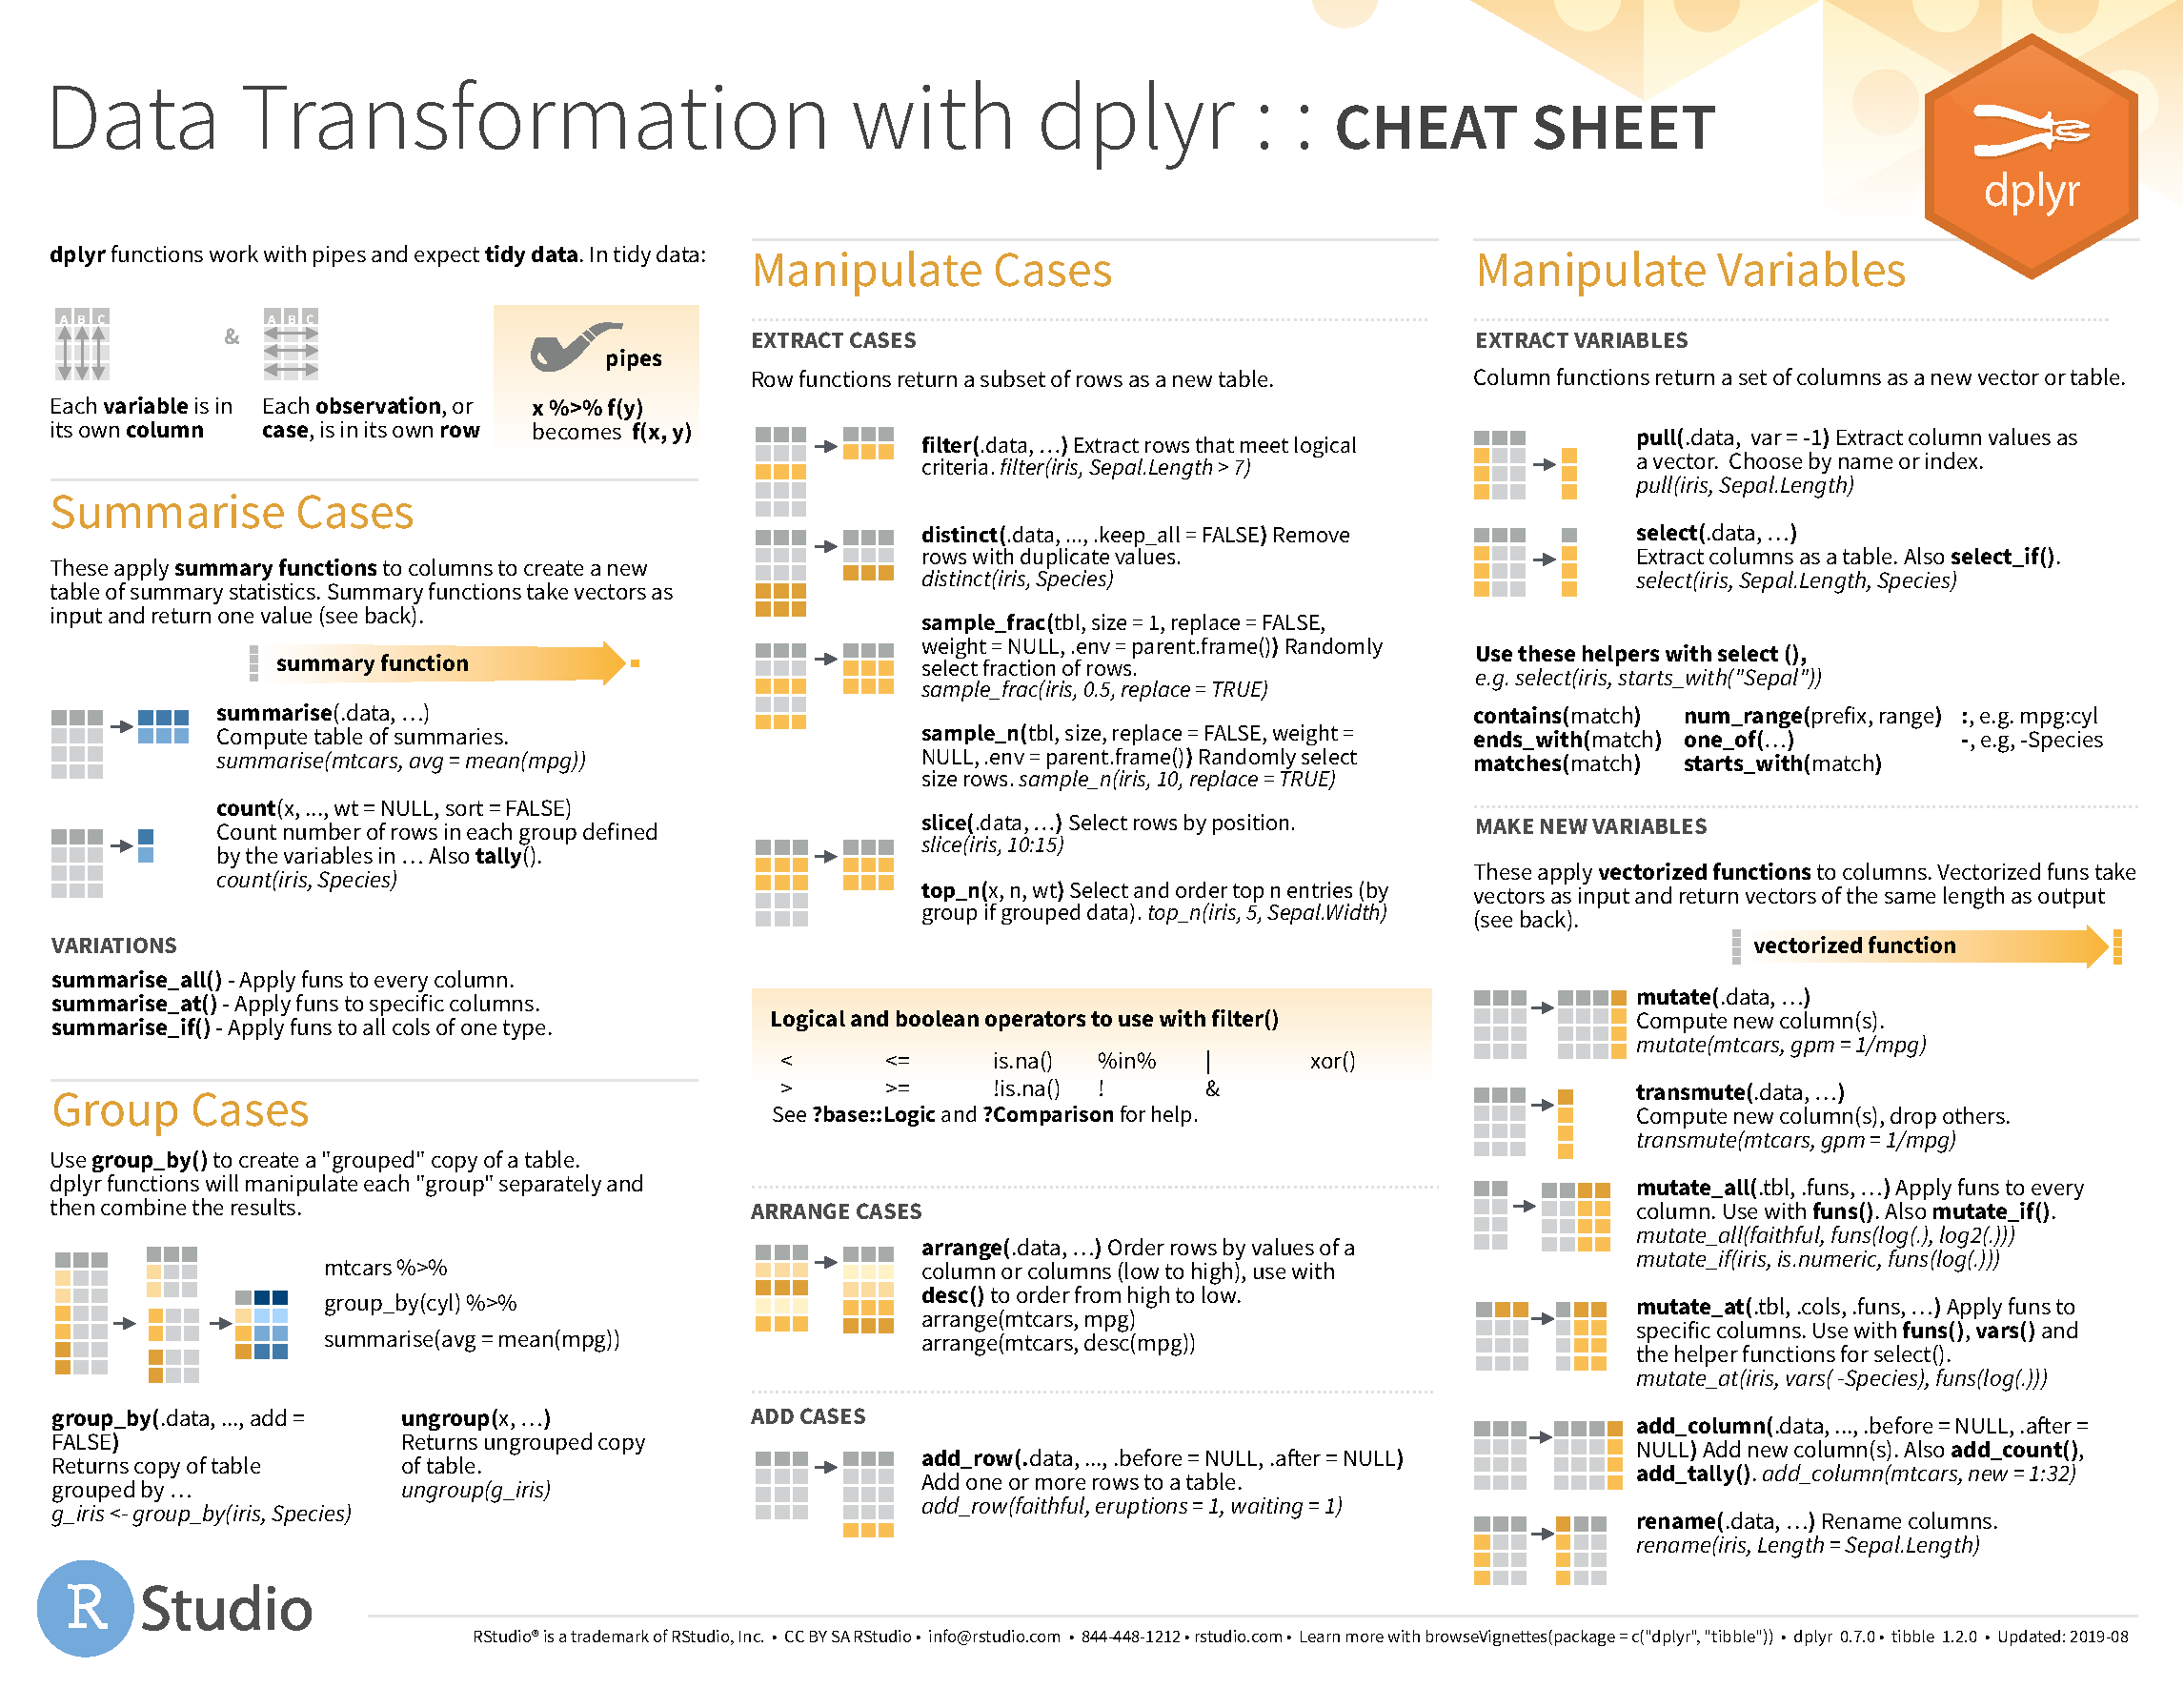
\includegraphics[width=1\textwidth,height=4.16667in]{./picture/dplyr/data-transformation.pdf}
\caption{dplyr-sheet}
\end{figure}

Rstudio其它手册:\url{https://www.rstudio.com/resources/cheatsheets/}

\hypertarget{ux57faux7840ux7528ux6cd5}{%
\section{基础用法}\label{ux57faux7840ux7528ux6cd5}}

基础用法部分,我们将从行筛选,重命名、列位置调整、新增计算列、排序、分组聚合几个方面阐述\texttt{dplyr}动词功能。

\hypertarget{ux52a0ux8f7dux5305}{%
\subsection{加载包}\label{ux52a0ux8f7dux5305}}

\begin{Shaded}
\begin{Highlighting}[]
\CommentTok{\#library(dplyr)}
\CommentTok{\# 禁掉提示}
\FunctionTok{library}\NormalTok{(dplyr,}\AttributeTok{warn.conflicts =} \ConstantTok{FALSE}\NormalTok{)}
\end{Highlighting}
\end{Shaded}

\hypertarget{filter}{%
\subsection{filter}\label{filter}}

\texttt{filter}动词顾名思义即筛选功能,按照一定条件筛选data.frame;与Excel中的筛选功能和\texttt{SQL}中\texttt{where}条件一致。

filter条件筛选中可以分为单条件筛选和多条件筛选;多条件中间用\texttt{,}分隔。

\begin{itemize}
\tightlist
\item
  单条件
\end{itemize}

条件为\texttt{species\ ==\ "Droid"}时,如下所示:

\begin{Shaded}
\begin{Highlighting}[]
\NormalTok{starwars }\SpecialCharTok{\%\textgreater{}\%} 
  \FunctionTok{filter}\NormalTok{(species }\SpecialCharTok{==} \StringTok{"Droid"}\NormalTok{)}
\end{Highlighting}
\end{Shaded}

\begin{Shaded}
\begin{Highlighting}[]
\KeywordTok{select} \OperatorTok{*} \KeywordTok{from}\NormalTok{ starwars }\KeywordTok{where}\NormalTok{ species }\OperatorTok{=} \OtherTok{"Droid"} \CommentTok{{-}{-} 注意=与==的区别}
\end{Highlighting}
\end{Shaded}

\begin{itemize}
\tightlist
\item
  多条件
\end{itemize}

多条件筛选时,用英文逗号隔开多个条件。用``and''连接多个条件与用逗号隔开效果相同,``and''在R中用\&表示。

\begin{Shaded}
\begin{Highlighting}[]
\NormalTok{starwars }\SpecialCharTok{\%\textgreater{}\%} 
  \FunctionTok{filter}\NormalTok{(species }\SpecialCharTok{==} \StringTok{"Droid"}\NormalTok{,skin\_color }\SpecialCharTok{==} \StringTok{"gold"}\NormalTok{)}

\CommentTok{\# same above}
\CommentTok{\# starwars \%\textgreater{}\% }
\CommentTok{\#   filter(species == "Droid" \& skin\_color == "gold")}
\end{Highlighting}
\end{Shaded}

\begin{Shaded}
\begin{Highlighting}[]
\KeywordTok{select} \OperatorTok{*} \KeywordTok{from}\NormalTok{ starwars }\KeywordTok{where}\NormalTok{ species }\OperatorTok{=} \OtherTok{"Droid"} \KeywordTok{and}\NormalTok{ skin\_color }\OperatorTok{=} \OtherTok{"gold"} 
\end{Highlighting}
\end{Shaded}

\begin{itemize}
\tightlist
\item
  多情况筛选
\end{itemize}

类似\texttt{SQL}中 \texttt{in} 的用法,或Excel中筛选条件时``或''条件

\begin{Shaded}
\begin{Highlighting}[]
\NormalTok{starwars }\SpecialCharTok{\%\textgreater{}\%} 
  \FunctionTok{filter}\NormalTok{(species }\SpecialCharTok{\%in\%}  \FunctionTok{c}\NormalTok{(}\StringTok{"Droid"}\NormalTok{,}\StringTok{\textquotesingle{}Clawdite\textquotesingle{}}\NormalTok{))}
\end{Highlighting}
\end{Shaded}

\begin{Shaded}
\begin{Highlighting}[]
\KeywordTok{select} \OperatorTok{*} \KeywordTok{from}\NormalTok{ starwars }\KeywordTok{where}\NormalTok{ species }\KeywordTok{in}\NormalTok{ (}\OtherTok{"Droid"}\NormalTok{,}\OtherTok{"Clawdite"}\NormalTok{) }\CommentTok{{-}{-}sql查询}
\end{Highlighting}
\end{Shaded}

\begin{itemize}
\tightlist
\item
  逻辑关系筛选
\end{itemize}

条件运算分为逻辑运算、关系运算。
关系运算符 \textgreater、\textless、==、!=、\textgreater=、\textless=分别代表大于、小于、等于、不等于、大于等于、小于等于。

逻辑运算符 \&、\textbar、!。 \texttt{\textbar{}}为 或, \texttt{\&} 为并、且条件,\texttt{!}为非。

\begin{Shaded}
\begin{Highlighting}[]
\FunctionTok{library}\NormalTok{(nycflights13)}
\FunctionTok{filter}\NormalTok{(flights, }\SpecialCharTok{!}\NormalTok{(arr\_delay }\SpecialCharTok{\textgreater{}} \DecValTok{120} \SpecialCharTok{|}\NormalTok{ dep\_delay }\SpecialCharTok{\textgreater{}} \DecValTok{120}\NormalTok{))}
\FunctionTok{filter}\NormalTok{(flights, arr\_delay }\SpecialCharTok{\textless{}=} \DecValTok{120}\NormalTok{, dep\_delay }\SpecialCharTok{\textless{}=} \DecValTok{120}\NormalTok{)}

\CommentTok{\# same above}
\FunctionTok{filter}\NormalTok{(flights, arr\_delay }\SpecialCharTok{\textless{}=} \DecValTok{120} \SpecialCharTok{\&}\NormalTok{ dep\_delay }\SpecialCharTok{\textless{}=} \DecValTok{120}\NormalTok{)}

\CommentTok{\# \%in\% 的反面}
\NormalTok{starwars }\SpecialCharTok{\%\textgreater{}\%} 
  \FunctionTok{filter}\NormalTok{(}\SpecialCharTok{!}\NormalTok{species }\SpecialCharTok{\%in\%}  \FunctionTok{c}\NormalTok{(}\StringTok{"Droid"}\NormalTok{,}\StringTok{\textquotesingle{}Clawdite\textquotesingle{}}\NormalTok{))}
\end{Highlighting}
\end{Shaded}

\begin{quote}
!的运算级别相比 \%in\% 更高
\end{quote}

\hypertarget{select}{%
\subsection{select}\label{select}}

当完整数据集列数较多时,我们某次分析可能并不需要那么多列,通过动词\texttt{select()}筛选列

\begin{itemize}
\tightlist
\item
  基础用法
\end{itemize}

通过指定列名称筛选,并指定列之间顺序

\begin{Shaded}
\begin{Highlighting}[]
\NormalTok{starwars }\SpecialCharTok{\%\textgreater{}\%} 
  \FunctionTok{select}\NormalTok{(name,height,mass,hair\_color,skin\_color,eye\_color)}
\end{Highlighting}
\end{Shaded}

\begin{itemize}
\tightlist
\item
  列索引
\end{itemize}

通过列名或数字向量索引,但是不建议用数字索引,避免原始数据列顺序变化后导致报错。

\begin{Shaded}
\begin{Highlighting}[]
\NormalTok{starwars }\SpecialCharTok{\%\textgreater{}\%} 
  \FunctionTok{select}\NormalTok{(name }\SpecialCharTok{:}\NormalTok{ eye\_color)}
\CommentTok{\#same above}
\NormalTok{starwars }\SpecialCharTok{\%\textgreater{}\%} 
  \FunctionTok{select}\NormalTok{(}\DecValTok{1}\SpecialCharTok{:}\DecValTok{6}\NormalTok{)}
\CommentTok{\# starwars \%\textgreater{}\% }
\CommentTok{\#   select(c(1,2,4,5,7))}
\end{Highlighting}
\end{Shaded}

\hypertarget{rename}{%
\subsection{rename}\label{rename}}

列重命名使用\texttt{rename()}函数,新名称写前面,如下所示:

\begin{Shaded}
\begin{Highlighting}[]
\NormalTok{starwars }\SpecialCharTok{\%\textgreater{}\%} \FunctionTok{rename}\NormalTok{(}\AttributeTok{home\_world =}\NormalTok{ homeworld)}
\CommentTok{\# 多列同换}
\NormalTok{starwars }\SpecialCharTok{\%\textgreater{}\%} \FunctionTok{rename}\NormalTok{(}\AttributeTok{home\_world =}\NormalTok{ homeworld,}\AttributeTok{skincolor =}\NormalTok{ skin\_color)}
\end{Highlighting}
\end{Shaded}

\begin{Shaded}
\begin{Highlighting}[]
\KeywordTok{select} \OperatorTok{*}\NormalTok{ ,homeworld }\KeywordTok{as}\NormalTok{ home\_word }\KeywordTok{from}\NormalTok{ starwars }
\KeywordTok{select} \OperatorTok{*}\NormalTok{ ,homeworld  home\_word }\KeywordTok{from}\NormalTok{ starwars }
\end{Highlighting}
\end{Shaded}

\begin{quote}
as 可以省略,但中间有一个以上空格。与R的差异是新增home\_word列,原始列继续存在,R中是替换列名。
\end{quote}

\hypertarget{relocate}{%
\subsection{relocate}\label{relocate}}

更改列顺序,与使用\texttt{select()}动词指定列顺序功能相似。

参数

\begin{Shaded}
\begin{Highlighting}[]
\FunctionTok{relocate}\NormalTok{(.data, ..., }\AttributeTok{.before =} \ConstantTok{NULL}\NormalTok{, }\AttributeTok{.after =} \ConstantTok{NULL}\NormalTok{)}
\end{Highlighting}
\end{Shaded}

\begin{Shaded}
\begin{Highlighting}[]
\CommentTok{\# sex:homeworld列在height列前面}
\NormalTok{starwars }\SpecialCharTok{\%\textgreater{}\%} \FunctionTok{relocate}\NormalTok{(sex}\SpecialCharTok{:}\NormalTok{homeworld, }\AttributeTok{.before =}\NormalTok{ height)}
\end{Highlighting}
\end{Shaded}

\hypertarget{mutate}{%
\subsection{mutate}\label{mutate}}

动词\texttt{mutate}

\begin{itemize}
\tightlist
\item
  新增计算列
\end{itemize}

\begin{Shaded}
\begin{Highlighting}[]
\NormalTok{starwars }\SpecialCharTok{\%\textgreater{}\%} 
  \FunctionTok{mutate}\NormalTok{(}\AttributeTok{bmi =}\NormalTok{ mass }\SpecialCharTok{/}\NormalTok{ ((height }\SpecialCharTok{/} \DecValTok{100}\NormalTok{)  }\SpecialCharTok{\^{}} \DecValTok{2}\NormalTok{)) }\SpecialCharTok{\%\textgreater{}\%} 
  \FunctionTok{select}\NormalTok{(name}\SpecialCharTok{:}\NormalTok{mass,bmi)}
\end{Highlighting}
\end{Shaded}

\begin{itemize}
\tightlist
\item
  新增计算列基础上新增列
\end{itemize}

\begin{Shaded}
\begin{Highlighting}[]
\NormalTok{starwars }\SpecialCharTok{\%\textgreater{}\%} 
  \FunctionTok{mutate}\NormalTok{(}\AttributeTok{bmi =}\NormalTok{ mass }\SpecialCharTok{/}\NormalTok{ ((height }\SpecialCharTok{/} \DecValTok{100}\NormalTok{)  }\SpecialCharTok{\^{}} \DecValTok{2}\NormalTok{),}\AttributeTok{newbmi =}\NormalTok{ bmi }\SpecialCharTok{*}\DecValTok{2}\NormalTok{) }\SpecialCharTok{\%\textgreater{}\%} 
  \FunctionTok{select}\NormalTok{(name}\SpecialCharTok{:}\NormalTok{mass,bmi,newbmi)}
\end{Highlighting}
\end{Shaded}

\begin{itemize}
\tightlist
\item
  删除列
\end{itemize}

\begin{Shaded}
\begin{Highlighting}[]
\NormalTok{starwars }\SpecialCharTok{\%\textgreater{}\%} \FunctionTok{mutate}\NormalTok{(}\AttributeTok{height =} \ConstantTok{NULL}\NormalTok{)}
\end{Highlighting}
\end{Shaded}

\hypertarget{arrange}{%
\subsection{arrange}\label{arrange}}

\begin{itemize}
\tightlist
\item
  单列排序,默认升序,通过\texttt{desc()}降序排列
\end{itemize}

\begin{Shaded}
\begin{Highlighting}[]
\NormalTok{starwars }\SpecialCharTok{\%\textgreater{}\%} 
  \FunctionTok{arrange}\NormalTok{(}\FunctionTok{desc}\NormalTok{(mass))}
\end{Highlighting}
\end{Shaded}

\begin{itemize}
\tightlist
\item
  多列排序
\end{itemize}

\begin{Shaded}
\begin{Highlighting}[]
\NormalTok{starwars }\SpecialCharTok{\%\textgreater{}\%} 
  \FunctionTok{arrange}\NormalTok{(height,}\FunctionTok{desc}\NormalTok{(mass))}
\end{Highlighting}
\end{Shaded}

\begin{Shaded}
\begin{Highlighting}[]
\KeywordTok{select} \OperatorTok{*} \KeywordTok{from}\NormalTok{ starwars }\KeywordTok{order} \KeywordTok{by}\NormalTok{ height,mass }\KeywordTok{desc}
\end{Highlighting}
\end{Shaded}

\hypertarget{summarise}{%
\subsection{summarise}\label{summarise}}

\texttt{summarise}常与\texttt{group\_by}结合使用。

\begin{Shaded}
\begin{Highlighting}[]
\NormalTok{mtcars }\SpecialCharTok{\%\textgreater{}\%}
  \FunctionTok{summarise}\NormalTok{(}\AttributeTok{mean =} \FunctionTok{mean}\NormalTok{(disp), }\AttributeTok{n =} \FunctionTok{n}\NormalTok{())}
\end{Highlighting}
\end{Shaded}

\begin{quote}
n()是dplyr包中的计算当前组的大小,用在summarise()和mutate()中。通常可用来组计算。
\end{quote}

\hypertarget{group_by}{%
\subsection{group\_by}\label{group_by}}

聚合前一般都需要分组,\texttt{group\_by()}动词实现该功能,与\texttt{SQL}中\texttt{group\ by\ ···}类似。

\begin{Shaded}
\begin{Highlighting}[]
\NormalTok{starwars }\SpecialCharTok{\%\textgreater{}\%}
  \FunctionTok{group\_by}\NormalTok{(species) }\SpecialCharTok{\%\textgreater{}\%}
  \FunctionTok{summarise}\NormalTok{(}
    \AttributeTok{n =} \FunctionTok{n}\NormalTok{(),}
    \AttributeTok{mass =} \FunctionTok{mean}\NormalTok{(mass, }\AttributeTok{na.rm =} \ConstantTok{TRUE}\NormalTok{)}
\NormalTok{  )}
\end{Highlighting}
\end{Shaded}

\begin{Shaded}
\begin{Highlighting}[]
\KeywordTok{SELECT}\NormalTok{ species,}
  \FunctionTok{count}\NormalTok{(species) n,}
  \FunctionTok{AVG}\NormalTok{(mass) mass}
\KeywordTok{FROM}\NormalTok{ [spb].[dbo].[starwars]}
\KeywordTok{GROUP} \KeywordTok{BY}\NormalTok{  species}
\end{Highlighting}
\end{Shaded}

\hypertarget{ux8868ux64cdux4f5c}{%
\section{表操作}\label{ux8868ux64cdux4f5c}}

\begin{enumerate}
\def\labelenumi{\arabic{enumi}.}
\item
  指像\texttt{sql}中的\texttt{left\ join},\texttt{inner\ join}等表格之间的操作,或者是Excel中\texttt{Power\ Piovt}建模的建立关系,从而实现不同表格间的关联
\item
  表格中的列操作,如列求和,均值等
\item
  行操作指不同字段间的计算,如\texttt{Excle}的列与列之间计算,\texttt{Excle}中的函数对行列不敏感,没有明显区别,但是\texttt{R}中\texttt{tidyverse}里列计算简单,行间计算依赖\texttt{rowwise()}函数实现
\end{enumerate}

\hypertarget{ux57faux7840}{%
\subsection{基础}\label{ux57faux7840}}

\texttt{left\_join()},\texttt{full\_join},\texttt{inner\_join()}等动词关联两个表。详情请查看:\texttt{vignette("two-table")}

\texttt{left\_join()}实现类似Excel中\texttt{VLOOKUP}函数功能或数据库中\texttt{left\ join}功能,将``右表''的字段依据``主键''关联到``左表''上。

\begin{itemize}
\tightlist
\item
  基础用法
\end{itemize}

\texttt{left\_join()},\texttt{right\_join()},\texttt{full\_join()},\texttt{inner\_join}(),第一个以左表为主,第二个右表为主,第三个全连接,第四个内连接(只返回两表中都有的记录),和数据库中连接方式一致。

默认会自动寻找两表中相同的字段名作为关联的条件

\begin{Shaded}
\begin{Highlighting}[]
\FunctionTok{library}\NormalTok{(}\StringTok{"nycflights13"}\NormalTok{)}
\CommentTok{\# Drop unimportant variables so it\textquotesingle{}s easier to understand the join results.}
\NormalTok{flights2 }\OtherTok{\textless{}{-}}\NormalTok{ flights }\SpecialCharTok{\%\textgreater{}\%} \FunctionTok{select}\NormalTok{(year}\SpecialCharTok{:}\NormalTok{day, hour, origin, dest, tailnum, carrier)}

\NormalTok{flights2 }\SpecialCharTok{\%\textgreater{}\%} 
  \FunctionTok{left\_join}\NormalTok{(airlines)}
\end{Highlighting}
\end{Shaded}

指定关联条件列,类似数据库中\texttt{on\ a.column\ =\ b.column}

\begin{Shaded}
\begin{Highlighting}[]
\NormalTok{flights2 }\SpecialCharTok{\%\textgreater{}\%} \FunctionTok{left\_join}\NormalTok{(planes, }\AttributeTok{by =} \StringTok{"tailnum"}\NormalTok{)}
\end{Highlighting}
\end{Shaded}

\begin{itemize}
\tightlist
\item
  不同名称列关联
\end{itemize}

\texttt{left\_join(x,y,by\ =\ c("a"\ =\ "b",\ "c"\ =\ "d"))} 将会匹配 x\(a to y\)b 和 x\(c to y\)d 作为关联条件

\begin{Shaded}
\begin{Highlighting}[]
\CommentTok{\#出发机场和目的机场信息}
\NormalTok{flights2 }\SpecialCharTok{\%\textgreater{}\%} \FunctionTok{left\_join}\NormalTok{(airports, }\AttributeTok{by =} \FunctionTok{c}\NormalTok{(}\StringTok{"dest"} \OtherTok{=} \StringTok{"faa"}\NormalTok{))}
\CommentTok{\#flights2 \%\textgreater{}\% left\_join(airports, c("origin" = "faa"))}
\CommentTok{\# 组合条件 多条件时用向量包裹即可c("dest" = "faa","cola" = "colb"))}
\end{Highlighting}
\end{Shaded}

\begin{itemize}
\tightlist
\item
  筛选连接
\end{itemize}

\texttt{anti\_join()} 删除所有左表中在右表中匹配到的行

\texttt{semi\_join()}保留所有左表在右表中匹配到的行

\begin{Shaded}
\begin{Highlighting}[]
\NormalTok{df1 }\OtherTok{\textless{}{-}} \FunctionTok{tibble}\NormalTok{(}\AttributeTok{a=}\NormalTok{letters[}\DecValTok{1}\SpecialCharTok{:}\DecValTok{20}\NormalTok{],}\AttributeTok{b=}\DecValTok{1}\SpecialCharTok{:}\DecValTok{20}\NormalTok{)}
\NormalTok{df2 }\OtherTok{\textless{}{-}} \FunctionTok{tibble}\NormalTok{(}\AttributeTok{a=}\NormalTok{letters,}\AttributeTok{b=}\DecValTok{1}\SpecialCharTok{:}\DecValTok{26}\NormalTok{)}

\NormalTok{df1 }\SpecialCharTok{\%\textgreater{}\%} \FunctionTok{semi\_join}\NormalTok{(df2)}
\NormalTok{df2 }\SpecialCharTok{\%\textgreater{}\%} \FunctionTok{anti\_join}\NormalTok{(df1)}
\end{Highlighting}
\end{Shaded}

\begin{itemize}
\tightlist
\item
  集合操作
\end{itemize}

\begin{enumerate}
\def\labelenumi{\arabic{enumi}.}
\item
  \texttt{intersect(x,y)}返回x,y交集
\item
  \texttt{union(x,y)}返回x,y中唯一的值
\item
  \texttt{setdiff(x,y)}返回存在x中但是不存在y中的记录
\end{enumerate}

\begin{Shaded}
\begin{Highlighting}[]
\NormalTok{(df1 }\OtherTok{\textless{}{-}} \FunctionTok{tibble}\NormalTok{(}\AttributeTok{x =} \DecValTok{1}\SpecialCharTok{:}\DecValTok{2}\NormalTok{, }\AttributeTok{y =} \FunctionTok{c}\NormalTok{(1L, 1L)))}
\NormalTok{(df2 }\OtherTok{\textless{}{-}} \FunctionTok{tibble}\NormalTok{(}\AttributeTok{x =} \DecValTok{1}\SpecialCharTok{:}\DecValTok{2}\NormalTok{, }\AttributeTok{y =} \DecValTok{1}\SpecialCharTok{:}\DecValTok{2}\NormalTok{))}
\FunctionTok{intersect}\NormalTok{(df1, df2)}
\FunctionTok{union}\NormalTok{(df1, df2)}
\FunctionTok{setdiff}\NormalTok{(df1, df2)}
\FunctionTok{setdiff}\NormalTok{(df2, df1)}
\end{Highlighting}
\end{Shaded}

\hypertarget{ux591aux8868ux64cdux4f5c}{%
\subsection{多表操作}\label{ux591aux8868ux64cdux4f5c}}

多表操作请使用\texttt{purrr::reduce()},当需要合并多个表格时,可用以下方式减少合并代码量。

\begin{Shaded}
\begin{Highlighting}[]
\NormalTok{dt1 }\OtherTok{\textless{}{-}} \FunctionTok{data.frame}\NormalTok{(}\AttributeTok{x =}\NormalTok{ letters)}
\NormalTok{dt2 }\OtherTok{\textless{}{-}} \FunctionTok{data.frame}\NormalTok{(}\AttributeTok{x =}\NormalTok{ letters,}\AttributeTok{cola =} \DecValTok{1}\SpecialCharTok{:}\DecValTok{26}\NormalTok{)}
\NormalTok{dt3 }\OtherTok{\textless{}{-}} \FunctionTok{data.frame}\NormalTok{(}\AttributeTok{x =}\NormalTok{ letters,}\AttributeTok{colb =} \DecValTok{1}\SpecialCharTok{:}\DecValTok{26}\NormalTok{)}
\NormalTok{dt4 }\OtherTok{\textless{}{-}} \FunctionTok{data.frame}\NormalTok{(}\AttributeTok{x =}\NormalTok{ letters,}\AttributeTok{cold =} \DecValTok{1}\SpecialCharTok{:}\DecValTok{26}\NormalTok{)}
\NormalTok{dt5 }\OtherTok{\textless{}{-}} \FunctionTok{data.frame}\NormalTok{(}\AttributeTok{x =}\NormalTok{ letters,}\AttributeTok{cole =} \DecValTok{1}\SpecialCharTok{:}\DecValTok{26}\NormalTok{)}

\NormalTok{dtlist }\OtherTok{\textless{}{-}} \FunctionTok{list}\NormalTok{(dt1,dt2,dt3,dt4,dt5)}
\NormalTok{purrr}\SpecialCharTok{::}\FunctionTok{reduce}\NormalTok{(dtlist,left\_join,}\AttributeTok{by=}\StringTok{\textquotesingle{}x\textquotesingle{}}\NormalTok{)}
\end{Highlighting}
\end{Shaded}

\hypertarget{ux5217ux64cdux4f5c}{%
\section{列操作}\label{ux5217ux64cdux4f5c}}

在多列上执行相同的操作是常用的操作,但是通过复制和粘贴代码,麻烦不说还容易错:

\begin{Shaded}
\begin{Highlighting}[]
\NormalTok{df }\SpecialCharTok{\%\textgreater{}\%} 
  \FunctionTok{group\_by}\NormalTok{(g1, g2) }\SpecialCharTok{\%\textgreater{}\%} 
  \FunctionTok{summarise}\NormalTok{(}\AttributeTok{a =} \FunctionTok{mean}\NormalTok{(a), }\AttributeTok{b =} \FunctionTok{mean}\NormalTok{(b), }\AttributeTok{c =} \FunctionTok{mean}\NormalTok{(c), }\AttributeTok{d =} \FunctionTok{mean}\NormalTok{(d))}
\end{Highlighting}
\end{Shaded}

通过\texttt{across()}函数可以更简洁地重写上面代码:

\begin{Shaded}
\begin{Highlighting}[]
\NormalTok{df }\SpecialCharTok{\%\textgreater{}\%} 
  \FunctionTok{group\_by}\NormalTok{(g1, g2) }\SpecialCharTok{\%\textgreater{}\%} 
  \FunctionTok{summarise}\NormalTok{(}\FunctionTok{across}\NormalTok{(a}\SpecialCharTok{:}\NormalTok{d, mean))}
\end{Highlighting}
\end{Shaded}

\hypertarget{ux57faux672cux64cdux4f5c}{%
\subsection{基本操作}\label{ux57faux672cux64cdux4f5c}}

across() 有两个主要参数:

\begin{itemize}
\item
  第一个参数,.cols选择要操作的列。它使用\texttt{tidyr}的方式选择(例如select()),因此您可以按位置,名称和类型选择变量。
\item
  第二个参数,.fns是要应用于每一列的一个函数或函数列表。这也可以是purrr样式的公式(或公式列表),例如\textasciitilde{} .x / 2。
\end{itemize}

\begin{Shaded}
\begin{Highlighting}[]
\NormalTok{starwars }\SpecialCharTok{\%\textgreater{}\%} 
  \FunctionTok{summarise}\NormalTok{(}\FunctionTok{across}\NormalTok{(}\FunctionTok{where}\NormalTok{(is.character), }\SpecialCharTok{\textasciitilde{}} \FunctionTok{length}\NormalTok{(}\FunctionTok{unique}\NormalTok{(.x))))}

\CommentTok{\# 列属性是字符的列求唯一值数}
\CommentTok{\# starwars \%\textgreater{}\% }
\CommentTok{\#   summarise(length(unique(name)))}
\CommentTok{\# starwars \%\textgreater{}\% }
\CommentTok{\#   summarise(length(unique(hair\_color)))}

\NormalTok{starwars }\SpecialCharTok{\%\textgreater{}\%} 
  \FunctionTok{group\_by}\NormalTok{(species) }\SpecialCharTok{\%\textgreater{}\%} 
  \FunctionTok{filter}\NormalTok{(}\FunctionTok{n}\NormalTok{() }\SpecialCharTok{\textgreater{}} \DecValTok{1}\NormalTok{) }\SpecialCharTok{\%\textgreater{}\%} 
  \FunctionTok{summarise}\NormalTok{(}\FunctionTok{across}\NormalTok{(}\FunctionTok{c}\NormalTok{(sex, gender, homeworld), }\SpecialCharTok{\textasciitilde{}} \FunctionTok{length}\NormalTok{(}\FunctionTok{unique}\NormalTok{(.x))))}

\NormalTok{starwars }\SpecialCharTok{\%\textgreater{}\%} 
  \FunctionTok{group\_by}\NormalTok{(homeworld) }\SpecialCharTok{\%\textgreater{}\%} 
  \FunctionTok{filter}\NormalTok{(}\FunctionTok{n}\NormalTok{() }\SpecialCharTok{\textgreater{}} \DecValTok{1}\NormalTok{) }\SpecialCharTok{\%\textgreater{}\%} 
  \FunctionTok{summarise}\NormalTok{(}\FunctionTok{across}\NormalTok{(}\FunctionTok{where}\NormalTok{(is.numeric), }\SpecialCharTok{\textasciitilde{}} \FunctionTok{mean}\NormalTok{(.x, }\AttributeTok{na.rm =} \ConstantTok{TRUE}\NormalTok{)))}
\end{Highlighting}
\end{Shaded}

\texttt{across()} 不会选择分组变量:

\begin{Shaded}
\begin{Highlighting}[]
\NormalTok{df }\OtherTok{\textless{}{-}} \FunctionTok{data.frame}\NormalTok{(}\AttributeTok{g =} \FunctionTok{c}\NormalTok{(}\DecValTok{1}\NormalTok{, }\DecValTok{1}\NormalTok{, }\DecValTok{2}\NormalTok{), }\AttributeTok{x =} \FunctionTok{c}\NormalTok{(}\SpecialCharTok{{-}}\DecValTok{1}\NormalTok{, }\DecValTok{1}\NormalTok{, }\DecValTok{3}\NormalTok{), }\AttributeTok{y =} \FunctionTok{c}\NormalTok{(}\SpecialCharTok{{-}}\DecValTok{1}\NormalTok{, }\SpecialCharTok{{-}}\DecValTok{4}\NormalTok{, }\SpecialCharTok{{-}}\DecValTok{9}\NormalTok{))}
\NormalTok{df }\SpecialCharTok{\%\textgreater{}\%} 
  \FunctionTok{group\_by}\NormalTok{(g) }\SpecialCharTok{\%\textgreater{}\%} 
  \FunctionTok{summarise}\NormalTok{(}\FunctionTok{across}\NormalTok{(}\FunctionTok{where}\NormalTok{(is.numeric), sum))}
\end{Highlighting}
\end{Shaded}

\hypertarget{ux591aux79cdux51fdux6570ux529fux80fd}{%
\subsection{多种函数功能}\label{ux591aux79cdux51fdux6570ux529fux80fd}}

通过在第二个参数提供函数或lambda函数的命名列表,可是使用多个函数转换每个变量:

\begin{Shaded}
\begin{Highlighting}[]
\NormalTok{min\_max }\OtherTok{\textless{}{-}} \FunctionTok{list}\NormalTok{(}
  \AttributeTok{min =} \SpecialCharTok{\textasciitilde{}}\FunctionTok{min}\NormalTok{(.x, }\AttributeTok{na.rm =} \ConstantTok{TRUE}\NormalTok{), }
  \AttributeTok{max =} \SpecialCharTok{\textasciitilde{}}\FunctionTok{max}\NormalTok{(.x, }\AttributeTok{na.rm =} \ConstantTok{TRUE}\NormalTok{)}
\NormalTok{)}
\NormalTok{starwars }\SpecialCharTok{\%\textgreater{}\%} \FunctionTok{summarise}\NormalTok{(}\FunctionTok{across}\NormalTok{(}\FunctionTok{where}\NormalTok{(is.numeric), min\_max))}
\end{Highlighting}
\end{Shaded}

通过\texttt{.names}参数控制名称:

NB:该参数的机制没有特别理解,需多练习体会。主要是运用到匿名函数时

以下是官方图册中的案例,但是报错:

\begin{Shaded}
\begin{Highlighting}[]
\NormalTok{starwars }\SpecialCharTok{\%\textgreater{}\%} \FunctionTok{summarise}\NormalTok{(}\FunctionTok{across}\NormalTok{(}\FunctionTok{where}\NormalTok{(is.numeric), min\_max, }\AttributeTok{.names =} \StringTok{"\{.fn\}.\{.col\}"}\NormalTok{))}
\end{Highlighting}
\end{Shaded}

修改后正常运行:

\begin{Shaded}
\begin{Highlighting}[]
\NormalTok{starwars }\SpecialCharTok{\%\textgreater{}\%} \FunctionTok{summarise}\NormalTok{(}\FunctionTok{across}\NormalTok{(}\FunctionTok{where}\NormalTok{(is.numeric), min\_max, }\AttributeTok{.names =} \StringTok{"\{fn\}.\{col\}"}\NormalTok{))}
\end{Highlighting}
\end{Shaded}

区别主要是\texttt{.names}参数的使用方式问题,\texttt{.}加不加的问题。

\begin{Shaded}
\begin{Highlighting}[]

\NormalTok{starwars }\SpecialCharTok{\%\textgreater{}\%} \FunctionTok{summarise}\NormalTok{(}\FunctionTok{across}\NormalTok{(}\FunctionTok{where}\NormalTok{(is.numeric), min\_max, }\AttributeTok{.names =} \StringTok{"\{fn\}——\{col\}"}\NormalTok{))}
\end{Highlighting}
\end{Shaded}

\hypertarget{ux5f53ux524dux5217}{%
\subsection{当前列}\label{ux5f53ux524dux5217}}

如果需要,可以通过调用访问内部的``当前''列的名称\texttt{cur\_column()}。

该函数不是特别容易理解,需要多尝试使用加深认识。

\begin{Shaded}
\begin{Highlighting}[]
\NormalTok{df }\OtherTok{\textless{}{-}} \FunctionTok{tibble}\NormalTok{(}\AttributeTok{x =} \DecValTok{1}\SpecialCharTok{:}\DecValTok{3}\NormalTok{, }\AttributeTok{y =} \DecValTok{3}\SpecialCharTok{:}\DecValTok{5}\NormalTok{, }\AttributeTok{z =} \DecValTok{5}\SpecialCharTok{:}\DecValTok{7}\NormalTok{)}
\NormalTok{mult }\OtherTok{\textless{}{-}} \FunctionTok{list}\NormalTok{(}\AttributeTok{x =} \DecValTok{1}\NormalTok{, }\AttributeTok{y =} \DecValTok{10}\NormalTok{, }\AttributeTok{z =} \DecValTok{100}\NormalTok{)}

\NormalTok{df }\SpecialCharTok{\%\textgreater{}\%} \FunctionTok{mutate}\NormalTok{(}\FunctionTok{across}\NormalTok{(}\FunctionTok{all\_of}\NormalTok{(}\FunctionTok{names}\NormalTok{(mult)), }\SpecialCharTok{\textasciitilde{}}\NormalTok{ .x }\SpecialCharTok{*}\NormalTok{ mult[[}\FunctionTok{cur\_column}\NormalTok{()]]))}
\end{Highlighting}
\end{Shaded}

\hypertarget{ux884cux64cdux4f5c}{%
\section{行操作}\label{ux884cux64cdux4f5c}}

在操纵数据框中,\texttt{dplyr}等工具让我们对列操作相对简单,但是对行操作则困难些。

\hypertarget{ux6784ux9020ux6570ux636eux96c6}{%
\subsection{构造数据集}\label{ux6784ux9020ux6570ux636eux96c6}}

\begin{Shaded}
\begin{Highlighting}[]
\NormalTok{df }\OtherTok{\textless{}{-}} \FunctionTok{tibble}\NormalTok{(}\AttributeTok{x =} \DecValTok{1}\SpecialCharTok{:}\DecValTok{2}\NormalTok{, }\AttributeTok{y =} \DecValTok{3}\SpecialCharTok{:}\DecValTok{4}\NormalTok{, }\AttributeTok{z =} \DecValTok{5}\SpecialCharTok{:}\DecValTok{6}\NormalTok{)}
\NormalTok{df }\SpecialCharTok{\%\textgreater{}\%} \FunctionTok{rowwise}\NormalTok{()}
\end{Highlighting}
\end{Shaded}

像\texttt{group\_by()},\texttt{rowwise()}并没有做任何事情,它的作用是改变其他动词的工作方式:
比较以下代码中不的不同

\begin{Shaded}
\begin{Highlighting}[]
\NormalTok{df }\SpecialCharTok{\%\textgreater{}\%} \FunctionTok{mutate}\NormalTok{(}\AttributeTok{m =} \FunctionTok{mean}\NormalTok{(}\FunctionTok{c}\NormalTok{(x, y, z)))}
\NormalTok{df }\SpecialCharTok{\%\textgreater{}\%} \FunctionTok{rowwise}\NormalTok{() }\SpecialCharTok{\%\textgreater{}\%} \FunctionTok{mutate}\NormalTok{(}\AttributeTok{m =} \FunctionTok{mean}\NormalTok{(}\FunctionTok{c}\NormalTok{(x, y, z)))}
\end{Highlighting}
\end{Shaded}

\texttt{data.table}中的操作:

\begin{Shaded}
\begin{Highlighting}[]
\FunctionTok{library}\NormalTok{(data.table)}

\NormalTok{dt }\OtherTok{\textless{}{-}} \FunctionTok{data.table}\NormalTok{(}\AttributeTok{x =} \DecValTok{1}\SpecialCharTok{:}\DecValTok{2}\NormalTok{, }\AttributeTok{y =} \DecValTok{3}\SpecialCharTok{:}\DecValTok{4}\NormalTok{, }\AttributeTok{z =} \DecValTok{5}\SpecialCharTok{:}\DecValTok{6}\NormalTok{)}
\NormalTok{dt[,m}\SpecialCharTok{:}\ErrorTok{=}\FunctionTok{mean}\NormalTok{(}\FunctionTok{c}\NormalTok{(x,y,z))][]}
\NormalTok{dt[,m}\SpecialCharTok{:}\ErrorTok{=}\FunctionTok{mean}\NormalTok{(}\FunctionTok{c}\NormalTok{(x,y,z)),by}\OtherTok{=}\NormalTok{.(x)][]}
\end{Highlighting}
\end{Shaded}

您可以选择在调用中提供``标识符''变量\texttt{rowwise()}。这些变量在您调用时被保留\texttt{summarise()},因此它们的行为与传递给的分组变量有些相似\texttt{group\_by()}:

\begin{Shaded}
\begin{Highlighting}[]
\NormalTok{df }\OtherTok{\textless{}{-}} \FunctionTok{tibble}\NormalTok{(}\AttributeTok{name =} \FunctionTok{c}\NormalTok{(}\StringTok{"Mara"}\NormalTok{, }\StringTok{"Hadley"}\NormalTok{), }\AttributeTok{x =} \DecValTok{1}\SpecialCharTok{:}\DecValTok{2}\NormalTok{, }\AttributeTok{y =} \DecValTok{3}\SpecialCharTok{:}\DecValTok{4}\NormalTok{, }\AttributeTok{z =} \DecValTok{5}\SpecialCharTok{:}\DecValTok{6}\NormalTok{)}

\NormalTok{df }\SpecialCharTok{\%\textgreater{}\%} 
  \FunctionTok{rowwise}\NormalTok{() }\SpecialCharTok{\%\textgreater{}\%} 
  \FunctionTok{summarise}\NormalTok{(}\AttributeTok{m =} \FunctionTok{mean}\NormalTok{(}\FunctionTok{c}\NormalTok{(x, y, z)))}

\NormalTok{df }\SpecialCharTok{\%\textgreater{}\%} 
  \FunctionTok{rowwise}\NormalTok{(name) }\SpecialCharTok{\%\textgreater{}\%} 
  \FunctionTok{summarise}\NormalTok{(}\AttributeTok{m =} \FunctionTok{mean}\NormalTok{(}\FunctionTok{c}\NormalTok{(x, y, z)))}
\end{Highlighting}
\end{Shaded}

\hypertarget{ux884cux6c47ux603bux7edfux8ba1}{%
\subsection{行汇总统计}\label{ux884cux6c47ux603bux7edfux8ba1}}

\texttt{dplyr::summarise()}使得汇总一列中各行的值非常容易。当与之结合使用时\texttt{rowwise()},还可以轻松汇总一行中各列的值:

\begin{Shaded}
\begin{Highlighting}[]
\NormalTok{df }\OtherTok{\textless{}{-}} \FunctionTok{tibble}\NormalTok{(}\AttributeTok{id =} \DecValTok{1}\SpecialCharTok{:}\DecValTok{6}\NormalTok{, }\AttributeTok{w =} \DecValTok{10}\SpecialCharTok{:}\DecValTok{15}\NormalTok{, }\AttributeTok{x =} \DecValTok{20}\SpecialCharTok{:}\DecValTok{25}\NormalTok{, }\AttributeTok{y =} \DecValTok{30}\SpecialCharTok{:}\DecValTok{35}\NormalTok{, }\AttributeTok{z =} \DecValTok{40}\SpecialCharTok{:}\DecValTok{45}\NormalTok{)}
\NormalTok{rf }\OtherTok{\textless{}{-}}\NormalTok{ df }\SpecialCharTok{\%\textgreater{}\%} \FunctionTok{rowwise}\NormalTok{(id)}
\NormalTok{rf }\SpecialCharTok{\%\textgreater{}\%} \FunctionTok{mutate}\NormalTok{(}\AttributeTok{total =} \FunctionTok{sum}\NormalTok{(}\FunctionTok{c}\NormalTok{(w, x, y, z)))}
\NormalTok{rf }\SpecialCharTok{\%\textgreater{}\%} \FunctionTok{summarise}\NormalTok{(}\AttributeTok{total =} \FunctionTok{sum}\NormalTok{(}\FunctionTok{c}\NormalTok{(w, x, y, z)))}
\end{Highlighting}
\end{Shaded}

键入每个变量名称很繁琐,通过\texttt{c\_across()}使更简单

\begin{Shaded}
\begin{Highlighting}[]
\NormalTok{rf }\SpecialCharTok{\%\textgreater{}\%} \FunctionTok{mutate}\NormalTok{(}\AttributeTok{total =} \FunctionTok{sum}\NormalTok{(}\FunctionTok{c\_across}\NormalTok{(w}\SpecialCharTok{:}\NormalTok{z)))}
\NormalTok{rf }\SpecialCharTok{\%\textgreater{}\%} \FunctionTok{mutate}\NormalTok{(}\AttributeTok{total =} \FunctionTok{sum}\NormalTok{(}\FunctionTok{c\_across}\NormalTok{(}\FunctionTok{where}\NormalTok{(is.numeric))))}

\NormalTok{rf }\SpecialCharTok{\%\textgreater{}\%} 
  \FunctionTok{mutate}\NormalTok{(}\AttributeTok{total =} \FunctionTok{sum}\NormalTok{(}\FunctionTok{c\_across}\NormalTok{(w}\SpecialCharTok{:}\NormalTok{z))) }\SpecialCharTok{\%\textgreater{}\%} 
  \FunctionTok{ungroup}\NormalTok{() }\SpecialCharTok{\%\textgreater{}\%} 
  \FunctionTok{mutate}\NormalTok{(}\FunctionTok{across}\NormalTok{(w}\SpecialCharTok{:}\NormalTok{z, }\SpecialCharTok{\textasciitilde{}}\NormalTok{ . }\SpecialCharTok{/}\NormalTok{ total))}
\end{Highlighting}
\end{Shaded}

\hypertarget{ux5206ux7ec4ux64cdux4f5c}{%
\section{分组操作}\label{ux5206ux7ec4ux64cdux4f5c}}

详情: \url{https://cloud.r-project.org/web/packages/dplyr/vignettes/grouping.html}

\texttt{group\_by()}最重要的分组动词,需要一个数据框和一个或多个变量进行分组:

\hypertarget{ux6dfbux52a0ux5206ux7ec4}{%
\subsection{添加分组}\label{ux6dfbux52a0ux5206ux7ec4}}

\begin{Shaded}
\begin{Highlighting}[]
\NormalTok{by\_species }\OtherTok{\textless{}{-}}\NormalTok{ starwars }\SpecialCharTok{\%\textgreater{}\%} \FunctionTok{group\_by}\NormalTok{(species)}
\NormalTok{by\_sex\_gender }\OtherTok{\textless{}{-}}\NormalTok{ starwars }\SpecialCharTok{\%\textgreater{}\%} \FunctionTok{group\_by}\NormalTok{(sex, gender)}
\end{Highlighting}
\end{Shaded}

除了按照现有变量分组外,还可以按照函数处理后的变量分组,等效在\texttt{mutate()}之后执行\texttt{group\_by}:

\begin{Shaded}
\begin{Highlighting}[]
\NormalTok{bmi\_breaks }\OtherTok{\textless{}{-}} \FunctionTok{c}\NormalTok{(}\DecValTok{0}\NormalTok{, }\FloatTok{18.5}\NormalTok{, }\DecValTok{25}\NormalTok{, }\DecValTok{30}\NormalTok{, }\ConstantTok{Inf}\NormalTok{)}
\NormalTok{starwars }\SpecialCharTok{\%\textgreater{}\%}
  \FunctionTok{group\_by}\NormalTok{(}\AttributeTok{bmi\_cat =} \FunctionTok{cut}\NormalTok{(mass}\SpecialCharTok{/}\NormalTok{(height}\SpecialCharTok{/}\DecValTok{100}\NormalTok{)}\SpecialCharTok{\^{}}\DecValTok{2}\NormalTok{, }\AttributeTok{breaks=}\NormalTok{bmi\_breaks)) }\SpecialCharTok{\%\textgreater{}\%}
  \FunctionTok{tally}\NormalTok{()}
\end{Highlighting}
\end{Shaded}

\hypertarget{ux5220ux9664ux5206ux7ec4ux53d8ux91cf}{%
\subsection{删除分组变量}\label{ux5220ux9664ux5206ux7ec4ux53d8ux91cf}}

要删除所有分组变量,使用\texttt{ungroup()}:

\begin{Shaded}
\begin{Highlighting}[]
\NormalTok{by\_species }\SpecialCharTok{\%\textgreater{}\%}
  \FunctionTok{ungroup}\NormalTok{() }\SpecialCharTok{\%\textgreater{}\%}
  \FunctionTok{tally}\NormalTok{()}
\end{Highlighting}
\end{Shaded}

\hypertarget{ux52a8ux8bcd}{%
\subsection{动词}\label{ux52a8ux8bcd}}

\texttt{summarise()} 计算每个组的汇总,表示从\texttt{group\_keys}开始右侧添加汇总变量

\begin{Shaded}
\begin{Highlighting}[]
\NormalTok{by\_species }\SpecialCharTok{\%\textgreater{}\%}
  \FunctionTok{summarise}\NormalTok{(}
    \AttributeTok{n =} \FunctionTok{n}\NormalTok{(),}
    \AttributeTok{height =} \FunctionTok{mean}\NormalTok{(height, }\AttributeTok{na.rm =} \ConstantTok{TRUE}\NormalTok{)}
\NormalTok{  )}
\end{Highlighting}
\end{Shaded}

该\texttt{.groups=}参数控制输出的分组结构。删除右侧分组变量的历史行为对应于\texttt{.groups\ =} ``drop\_last''没有消息或.groups = NULL有消息(默认值)。

从1.0.0版开始,分组信息可以保留\texttt{(.groups\ =\ "keep")}或删除 \texttt{(.groups\ =\ \textquotesingle{}drop)}

\begin{Shaded}
\begin{Highlighting}[]
\NormalTok{a }\OtherTok{\textless{}{-}}\NormalTok{ by\_species }\SpecialCharTok{\%\textgreater{}\%}
  \FunctionTok{summarise}\NormalTok{(}
    \AttributeTok{n =} \FunctionTok{n}\NormalTok{(),}
    \AttributeTok{height =} \FunctionTok{mean}\NormalTok{(height, }\AttributeTok{na.rm =} \ConstantTok{TRUE}\NormalTok{),}\AttributeTok{.groups=}\StringTok{\textquotesingle{}drop\textquotesingle{}}\NormalTok{) }\SpecialCharTok{\%\textgreater{}\%} 
  \FunctionTok{group\_vars}\NormalTok{()}

\NormalTok{b }\OtherTok{\textless{}{-}}\NormalTok{ by\_species }\SpecialCharTok{\%\textgreater{}\%}
  \FunctionTok{summarise}\NormalTok{(}
    \AttributeTok{n =} \FunctionTok{n}\NormalTok{(),}
    \AttributeTok{height =} \FunctionTok{mean}\NormalTok{(height, }\AttributeTok{na.rm =} \ConstantTok{TRUE}\NormalTok{),}\AttributeTok{.groups=}\StringTok{\textquotesingle{}keep\textquotesingle{}}\NormalTok{) }\SpecialCharTok{\%\textgreater{}\%} 
  \FunctionTok{group\_vars}\NormalTok{()}

\FunctionTok{object.size}\NormalTok{(a)}
\FunctionTok{object.size}\NormalTok{(b)}
\end{Highlighting}
\end{Shaded}

在实际使用中,当数据较大时需要删掉分组信息。以上可以看到保留分组信息的比没保留的大了两倍多。

\hypertarget{ux5e38ux7528ux51fdux6570}{%
\section{常用函数}\label{ux5e38ux7528ux51fdux6570}}

\hypertarget{ux6761ux4ef6ux5224ux65ad}{%
\subsection{条件判断}\label{ux6761ux4ef6ux5224ux65ad}}

相比于\texttt{base::ifelse},\texttt{if\_else}更为严格,无论\texttt{TRUE}或\texttt{FALSE}输出类型一致,这样速度更快。与\texttt{data.table::fifelse()}功能相似。

\begin{Shaded}
\begin{Highlighting}[]
\FunctionTok{if\_else}\NormalTok{(condition, true, false, }\AttributeTok{missing =} \ConstantTok{NULL}\NormalTok{)}
\end{Highlighting}
\end{Shaded}

与\texttt{ifelse}不同的是,\texttt{if\_else}保留类型

\begin{Shaded}
\begin{Highlighting}[]
\NormalTok{x }\OtherTok{\textless{}{-}} \FunctionTok{factor}\NormalTok{(}\FunctionTok{sample}\NormalTok{(letters[}\DecValTok{1}\SpecialCharTok{:}\DecValTok{5}\NormalTok{], }\DecValTok{10}\NormalTok{, }\AttributeTok{replace =} \ConstantTok{TRUE}\NormalTok{))}
\FunctionTok{ifelse}\NormalTok{(x }\SpecialCharTok{\%in\%} \FunctionTok{c}\NormalTok{(}\StringTok{"a"}\NormalTok{, }\StringTok{"b"}\NormalTok{, }\StringTok{"c"}\NormalTok{), x, }\FunctionTok{factor}\NormalTok{(}\ConstantTok{NA}\NormalTok{))}
\FunctionTok{if\_else}\NormalTok{(x }\SpecialCharTok{\%in\%} \FunctionTok{c}\NormalTok{(}\StringTok{"a"}\NormalTok{, }\StringTok{"b"}\NormalTok{, }\StringTok{"c"}\NormalTok{), x, }\FunctionTok{factor}\NormalTok{(}\ConstantTok{NA}\NormalTok{))}
\end{Highlighting}
\end{Shaded}

\hypertarget{case_when}{%
\subsection{case\_when}\label{case_when}}

当条件嵌套条件较多时,使用\texttt{case\_when},使代码可读并且不易出错。与sql 中的case when 等价。

\begin{Shaded}
\begin{Highlighting}[]
\NormalTok{Dates }\OtherTok{\textless{}{-}} \FunctionTok{as.Date}\NormalTok{(}\FunctionTok{c}\NormalTok{(}\StringTok{\textquotesingle{}2018{-}10{-}01\textquotesingle{}}\NormalTok{, }\StringTok{\textquotesingle{}2018{-}10{-}02\textquotesingle{}}\NormalTok{, }\StringTok{\textquotesingle{}2018{-}10{-}03\textquotesingle{}}\NormalTok{))}
\FunctionTok{case\_when}\NormalTok{(}
\NormalTok{  Dates }\SpecialCharTok{==} \StringTok{\textquotesingle{}2018{-}10{-}01\textquotesingle{}} \SpecialCharTok{\textasciitilde{}}\NormalTok{ Dates }\SpecialCharTok{{-}} \DecValTok{1}\NormalTok{,}
\NormalTok{  Dates }\SpecialCharTok{==} \StringTok{\textquotesingle{}2018{-}10{-}02\textquotesingle{}} \SpecialCharTok{\textasciitilde{}}\NormalTok{ Dates }\SpecialCharTok{+} \DecValTok{1}\NormalTok{,}
\NormalTok{  Dates }\SpecialCharTok{==} \StringTok{\textquotesingle{}2018{-}10{-}03\textquotesingle{}} \SpecialCharTok{\textasciitilde{}}\NormalTok{ Dates }\SpecialCharTok{+} \DecValTok{2}\NormalTok{,}
  \ConstantTok{TRUE} \SpecialCharTok{\textasciitilde{}}\NormalTok{ Dates}
\NormalTok{)}
\end{Highlighting}
\end{Shaded}

\hypertarget{ux8ba1ux6570ux51fdux6570}{%
\subsection{计数函数}\label{ux8ba1ux6570ux51fdux6570}}

\begin{itemize}
\tightlist
\item
  计数
\end{itemize}

\texttt{count()}函数用来计数。下面两种表达方式等价。

\begin{Shaded}
\begin{Highlighting}[]
\NormalTok{df }\SpecialCharTok{\%\textgreater{}\%} \FunctionTok{count}\NormalTok{(a, b)}
\CommentTok{\# same above}
\NormalTok{df }\SpecialCharTok{\%\textgreater{}\%} \FunctionTok{group\_by}\NormalTok{(a, b) }\SpecialCharTok{\%\textgreater{}\%} \FunctionTok{summarise}\NormalTok{(}\AttributeTok{n =} \FunctionTok{n}\NormalTok{())}
\end{Highlighting}
\end{Shaded}

\begin{Shaded}
\begin{Highlighting}[]
\NormalTok{starwars }\SpecialCharTok{\%\textgreater{}\%} \FunctionTok{count}\NormalTok{(species)}
\CommentTok{\# same above 等价}
\NormalTok{starwars }\SpecialCharTok{\%\textgreater{}\%} \FunctionTok{group\_by}\NormalTok{(species) }\SpecialCharTok{\%\textgreater{}\%} \FunctionTok{summarise}\NormalTok{(}\AttributeTok{n =} \FunctionTok{n}\NormalTok{())}
\end{Highlighting}
\end{Shaded}

\begin{itemize}
\tightlist
\item
  非重复计数
\end{itemize}

\texttt{n\_distinct()}与\texttt{length(unique(x))}等价,但是更快更简洁。当我们需要给门店或订单之类数据需要去重计算时采用该函数。

\begin{Shaded}
\begin{Highlighting}[]
\NormalTok{x }\OtherTok{\textless{}{-}} \FunctionTok{sample}\NormalTok{(}\DecValTok{1}\SpecialCharTok{:}\DecValTok{10}\NormalTok{, }\FloatTok{1e5}\NormalTok{, }\AttributeTok{rep =} \ConstantTok{TRUE}\NormalTok{)}
\FunctionTok{length}\NormalTok{(}\FunctionTok{unique}\NormalTok{(x))}
\FunctionTok{n\_distinct}\NormalTok{(x)}
\end{Highlighting}
\end{Shaded}

\hypertarget{ux6392ux5e8fux51fdux6570}{%
\subsection{排序函数}\label{ux6392ux5e8fux51fdux6570}}

\texttt{dplyr}共六种排序函数,模仿SQL2003中的排名函数。

\begin{itemize}
\tightlist
\item
  row\_number():等于 rank(ties.method = ``first'')
\item
  min\_rank(): 等于 rank(ties.method = ``min'')
\item
  dense\_rank(): 与min\_rank()相似,但是没有间隔
\item
  percent\_rank():返回0,1之间,通过min\_rank()返回值缩放至{[}0,1{]}
\end{itemize}

\begin{Shaded}
\begin{Highlighting}[]
\NormalTok{x }\OtherTok{\textless{}{-}} \FunctionTok{c}\NormalTok{(}\DecValTok{5}\NormalTok{, }\DecValTok{1}\NormalTok{, }\DecValTok{3}\NormalTok{, }\DecValTok{2}\NormalTok{, }\DecValTok{2}\NormalTok{, }\ConstantTok{NA}\NormalTok{)}
\FunctionTok{row\_number}\NormalTok{(x)}
\FunctionTok{min\_rank}\NormalTok{(x)}
\FunctionTok{dense\_rank}\NormalTok{(x)}
\FunctionTok{percent\_rank}\NormalTok{(x)}
\FunctionTok{cume\_dist}\NormalTok{(x)}
\end{Highlighting}
\end{Shaded}

\hypertarget{ux63d0ux53d6ux5411ux91cf}{%
\subsection{提取向量}\label{ux63d0ux53d6ux5411ux91cf}}

该系列函数是对\texttt{{[}{[}}的包装。

\begin{Shaded}
\begin{Highlighting}[]
\FunctionTok{nth}\NormalTok{(x, n, }\AttributeTok{order\_by =} \ConstantTok{NULL}\NormalTok{, }\AttributeTok{default =} \FunctionTok{default\_missing}\NormalTok{(x))}
\FunctionTok{first}\NormalTok{(x, }\AttributeTok{order\_by =} \ConstantTok{NULL}\NormalTok{, }\AttributeTok{default =} \FunctionTok{default\_missing}\NormalTok{(x))}
\FunctionTok{last}\NormalTok{(x, }\AttributeTok{order\_by =} \ConstantTok{NULL}\NormalTok{, }\AttributeTok{default =} \FunctionTok{default\_missing}\NormalTok{(x))}
\end{Highlighting}
\end{Shaded}

\begin{Shaded}
\begin{Highlighting}[]
\NormalTok{x }\OtherTok{\textless{}{-}} \DecValTok{1}\SpecialCharTok{:}\DecValTok{10}
\NormalTok{y }\OtherTok{\textless{}{-}} \DecValTok{10}\SpecialCharTok{:}\DecValTok{1}
\FunctionTok{first}\NormalTok{(x)}
\FunctionTok{last}\NormalTok{(y)}
\FunctionTok{nth}\NormalTok{(x, }\DecValTok{1}\NormalTok{)}
\FunctionTok{nth}\NormalTok{(x, }\DecValTok{5}\NormalTok{)}
\end{Highlighting}
\end{Shaded}

\hypertarget{group-ux7cfbux5217}{%
\subsection{group 系列}\label{group-ux7cfbux5217}}

group\_by(),group\_map(), group\_nest(), group\_split(), group\_trim()等一系列函数。

其中我常用group\_by(),group\_split()两个函数。group\_by()是大部分数据操作中的分组操作,按照group\_by()的指定分组条件。

\begin{itemize}
\tightlist
\item
  group\_by()
\end{itemize}

\begin{Shaded}
\begin{Highlighting}[]
\CommentTok{\#group\_by()不会改变数据框}
\NormalTok{by\_cyl }\OtherTok{\textless{}{-}}\NormalTok{ mtcars }\SpecialCharTok{\%\textgreater{}\%} \FunctionTok{group\_by}\NormalTok{(cyl)}
\NormalTok{by\_cyl}
\CommentTok{\# It changes how it acts with the other dplyr verbs:}
\NormalTok{by\_cyl }\SpecialCharTok{\%\textgreater{}\%} \FunctionTok{summarise}\NormalTok{(}
  \AttributeTok{disp =} \FunctionTok{mean}\NormalTok{(disp),}
  \AttributeTok{hp =} \FunctionTok{mean}\NormalTok{(hp)}
\NormalTok{)}
\CommentTok{\# group\_by中可以添加计算字段 即mutate操作}
\NormalTok{mtcars }\SpecialCharTok{\%\textgreater{}\%} \FunctionTok{group\_by}\NormalTok{(}\AttributeTok{vsam =}\NormalTok{ vs }\SpecialCharTok{+}\NormalTok{ am) }\SpecialCharTok{\%\textgreater{}\%}
  \FunctionTok{group\_vars}\NormalTok{()}
\end{Highlighting}
\end{Shaded}

\begin{itemize}
\tightlist
\item
  group\_map()
\end{itemize}

group\_map,group\_modify,group\_walk等三个函数是purrr类具有迭代风格的函数。简单关系数据库的数据清洗一般不涉及,常用在建模等方面。

但是目前三个函数是实验性的,未来可能会发生变化。

\begin{Shaded}
\begin{Highlighting}[]
\CommentTok{\# return a list}
\CommentTok{\# 返回列表}
\NormalTok{mtcars }\SpecialCharTok{\%\textgreater{}\%}
  \FunctionTok{group\_by}\NormalTok{(cyl) }\SpecialCharTok{\%\textgreater{}\%}
  \FunctionTok{group\_map}\NormalTok{(}\SpecialCharTok{\textasciitilde{}} \FunctionTok{head}\NormalTok{(.x, 2L))}
\end{Highlighting}
\end{Shaded}

\begin{Shaded}
\begin{Highlighting}[]
\NormalTok{iris }\SpecialCharTok{\%\textgreater{}\%}
  \FunctionTok{group\_by}\NormalTok{(Species) }\SpecialCharTok{\%\textgreater{}\%}
  \FunctionTok{group\_modify}\NormalTok{(}\SpecialCharTok{\textasciitilde{}}\NormalTok{ \{}
\NormalTok{    .x }\SpecialCharTok{\%\textgreater{}\%}
\NormalTok{      purrr}\SpecialCharTok{::}\FunctionTok{map\_dfc}\NormalTok{(fivenum) }\SpecialCharTok{\%\textgreater{}\%}
      \FunctionTok{mutate}\NormalTok{(}\AttributeTok{nms =} \FunctionTok{c}\NormalTok{(}\StringTok{"min"}\NormalTok{, }\StringTok{"Q1"}\NormalTok{, }\StringTok{"median"}\NormalTok{, }\StringTok{"Q3"}\NormalTok{, }\StringTok{"max"}\NormalTok{))}
\NormalTok{  \})}
\end{Highlighting}
\end{Shaded}

\begin{Shaded}
\begin{Highlighting}[]
\CommentTok{\# group\_walk}
\FunctionTok{dir.create}\NormalTok{(temp }\OtherTok{\textless{}{-}} \FunctionTok{tempfile}\NormalTok{())}
\NormalTok{iris }\SpecialCharTok{\%\textgreater{}\%}
  \FunctionTok{group\_by}\NormalTok{(Species) }\SpecialCharTok{\%\textgreater{}\%}
  \FunctionTok{group\_walk}\NormalTok{(}\SpecialCharTok{\textasciitilde{}} \FunctionTok{write.csv}\NormalTok{(.x, }\AttributeTok{file =} \FunctionTok{file.path}\NormalTok{(temp, }\FunctionTok{paste0}\NormalTok{(.y}\SpecialCharTok{$}\NormalTok{Species, }\StringTok{".csv"}\NormalTok{))))}
\FunctionTok{list.files}\NormalTok{(temp, }\AttributeTok{pattern =} \StringTok{"csv$"}\NormalTok{)}
\FunctionTok{unlink}\NormalTok{(temp, }\AttributeTok{recursive =} \ConstantTok{TRUE}\NormalTok{)}
\end{Highlighting}
\end{Shaded}

\begin{itemize}
\tightlist
\item
  group\_cols()
\end{itemize}

选择分组变量

\begin{Shaded}
\begin{Highlighting}[]
\NormalTok{gdf }\OtherTok{\textless{}{-}}\NormalTok{ iris }\SpecialCharTok{\%\textgreater{}\%} \FunctionTok{group\_by}\NormalTok{(Species)}
\NormalTok{gdf }\SpecialCharTok{\%\textgreater{}\%} \FunctionTok{select}\NormalTok{(}\FunctionTok{group\_cols}\NormalTok{())}
\end{Highlighting}
\end{Shaded}

\hypertarget{ux5176ux5b83ux51fdux6570}{%
\subsection{其它函数}\label{ux5176ux5b83ux51fdux6570}}

\begin{itemize}
\item
  between
\item
  cummean cumsum cumall cumany
\end{itemize}

累计系列函数

\begin{Shaded}
\begin{Highlighting}[]
\NormalTok{x }\OtherTok{\textless{}{-}} \FunctionTok{c}\NormalTok{(}\DecValTok{1}\NormalTok{, }\DecValTok{3}\NormalTok{, }\DecValTok{5}\NormalTok{, }\DecValTok{2}\NormalTok{, }\DecValTok{2}\NormalTok{)}
\FunctionTok{cummean}\NormalTok{(x)}
\FunctionTok{cumsum}\NormalTok{(x) }\SpecialCharTok{/} \FunctionTok{seq\_along}\NormalTok{(x)}

\FunctionTok{cumall}\NormalTok{(x }\SpecialCharTok{\textless{}} \DecValTok{5}\NormalTok{)}
\FunctionTok{cumany}\NormalTok{(x }\SpecialCharTok{==} \DecValTok{3}\NormalTok{)}
\end{Highlighting}
\end{Shaded}

\begin{itemize}
\tightlist
\item
  distinct
\end{itemize}

\begin{Shaded}
\begin{Highlighting}[]
\NormalTok{df }\OtherTok{\textless{}{-}} \FunctionTok{tibble}\NormalTok{(}
  \AttributeTok{x =} \FunctionTok{sample}\NormalTok{(}\DecValTok{10}\NormalTok{, }\DecValTok{100}\NormalTok{, }\AttributeTok{rep =} \ConstantTok{TRUE}\NormalTok{),}
  \AttributeTok{y =} \FunctionTok{sample}\NormalTok{(}\DecValTok{10}\NormalTok{, }\DecValTok{100}\NormalTok{, }\AttributeTok{rep =} \ConstantTok{TRUE}\NormalTok{)}
\NormalTok{)}

\FunctionTok{distinct}\NormalTok{(df, x)}
\FunctionTok{distinct}\NormalTok{(df, x, }\AttributeTok{.keep\_all =} \ConstantTok{TRUE}\NormalTok{)}
\FunctionTok{distinct}\NormalTok{(df, }\AttributeTok{diff =} \FunctionTok{abs}\NormalTok{(x }\SpecialCharTok{{-}}\NormalTok{ y))}
\end{Highlighting}
\end{Shaded}

\hypertarget{ux7528dplyrux7f16ux7a0b}{%
\section{\texorpdfstring{用\texttt{dplyr}编程}{用dplyr编程}}\label{ux7528dplyrux7f16ux7a0b}}

Programming with dplyr:

\url{https://cloud.r-project.org/web/packages/dplyr/vignettes/programming.html}

本节概念性东西较多且复杂不易理解,先尝试会使用,概念再慢慢消化理解。

虽然复杂但是比较实用,尤其是当我们需要定义一些通用功能函数时

以下是对原文引用

两种情况:

\begin{itemize}
\tightlist
\item
  When you have the data-variable in a function argument (i.e.~an env-variable that holds a promise2), you need to ** embrace ** the argument by surrounding it in doubled braces, like \texttt{filter(df,\ \{\{\ var\ \}\})}.
\end{itemize}

The following function uses embracing to create a wrapper around \texttt{summarise()} that computes the minimum and maximum values of a variable, as well as the number of observations that were summarised:

\begin{Shaded}
\begin{Highlighting}[]
\NormalTok{var\_summary }\OtherTok{\textless{}{-}} \ControlFlowTok{function}\NormalTok{(data, var) \{}
\NormalTok{  data }\SpecialCharTok{\%\textgreater{}\%}
    \FunctionTok{summarise}\NormalTok{(}\AttributeTok{n =} \FunctionTok{n}\NormalTok{(), }\AttributeTok{min =} \FunctionTok{min}\NormalTok{(\{\{ var \}\}), }\AttributeTok{max =} \FunctionTok{max}\NormalTok{(\{\{ var \}\}))}
\NormalTok{\}}
\NormalTok{mtcars }\SpecialCharTok{\%\textgreater{}\%} 
  \FunctionTok{group\_by}\NormalTok{(cyl) }\SpecialCharTok{\%\textgreater{}\%} 
  \FunctionTok{var\_summary}\NormalTok{(mpg)}
\end{Highlighting}
\end{Shaded}

\begin{itemize}
\tightlist
\item
  When you have an env-variable that is a character vector, you need to index into the .data pronoun with {[}{[}, like summarise(df, mean = mean(.data{[}{[}var{]}{]})).
\end{itemize}

The following example uses .data to count the number of unique values in each variable of mtcars:

\begin{Shaded}
\begin{Highlighting}[]
\ControlFlowTok{for}\NormalTok{ (var }\ControlFlowTok{in} \FunctionTok{names}\NormalTok{(mtcars)) \{}
\NormalTok{  mtcars }\SpecialCharTok{\%\textgreater{}\%} \FunctionTok{count}\NormalTok{(.data[[var]]) }\SpecialCharTok{\%\textgreater{}\%} \FunctionTok{print}\NormalTok{()}
\NormalTok{\}}
\end{Highlighting}
\end{Shaded}

Note that .data is not a data frame; it's a special construct, a pronoun, that allows you to access the current variables either directly, with \texttt{.data\$x} or indirectly with \texttt{.data{[}{[}var{]}{]}}. Don't expect other functions to work with it.

\hypertarget{ux6848ux4f8b}{%
\subsection{案例}\label{ux6848ux4f8b}}

当我们不知道接下来会用哪个变量汇总时:

\begin{Shaded}
\begin{Highlighting}[]
\NormalTok{my\_summarise }\OtherTok{\textless{}{-}} \ControlFlowTok{function}\NormalTok{(data, group\_var) \{}
\NormalTok{  data }\SpecialCharTok{\%\textgreater{}\%}
    \FunctionTok{group\_by}\NormalTok{(\{\{ group\_var \}\}) }\SpecialCharTok{\%\textgreater{}\%}
    \FunctionTok{summarise}\NormalTok{(}\AttributeTok{mean =} \FunctionTok{mean}\NormalTok{(mass))}
\NormalTok{\}}
\end{Highlighting}
\end{Shaded}

如果在多个位置使用:

\begin{Shaded}
\begin{Highlighting}[]
\NormalTok{my\_summarise2 }\OtherTok{\textless{}{-}} \ControlFlowTok{function}\NormalTok{(data, expr) \{}
\NormalTok{  data }\SpecialCharTok{\%\textgreater{}\%} \FunctionTok{summarise}\NormalTok{(}
    \AttributeTok{mean =} \FunctionTok{mean}\NormalTok{(\{\{ expr \}\}),}
    \AttributeTok{sum =} \FunctionTok{sum}\NormalTok{(\{\{ expr \}\}),}
    \AttributeTok{n =} \FunctionTok{n}\NormalTok{()}
\NormalTok{  )}
\NormalTok{\}}
\end{Highlighting}
\end{Shaded}

当多个表达式时:

\begin{Shaded}
\begin{Highlighting}[]
\NormalTok{my\_summarise3 }\OtherTok{\textless{}{-}} \ControlFlowTok{function}\NormalTok{(data, mean\_var, sd\_var) \{}
\NormalTok{  data }\SpecialCharTok{\%\textgreater{}\%} 
    \FunctionTok{summarise}\NormalTok{(}\AttributeTok{mean =} \FunctionTok{mean}\NormalTok{(\{\{ mean\_var \}\}), }\AttributeTok{sd =} \FunctionTok{mean}\NormalTok{(\{\{ sd\_var \}\}))}
\NormalTok{\}}
\end{Highlighting}
\end{Shaded}

如果要输出变量名时:

\begin{Shaded}
\begin{Highlighting}[]
\NormalTok{my\_summarise4 }\OtherTok{\textless{}{-}} \ControlFlowTok{function}\NormalTok{(data, expr) \{}
\NormalTok{  data }\SpecialCharTok{\%\textgreater{}\%} \FunctionTok{summarise}\NormalTok{(}
    \StringTok{"mean\_\{\{expr\}\}"} \SpecialCharTok{:}\ErrorTok{=} \FunctionTok{mean}\NormalTok{(\{\{ expr \}\}),}
    \StringTok{"sum\_\{\{expr\}\}"} \SpecialCharTok{:}\ErrorTok{=} \FunctionTok{sum}\NormalTok{(\{\{ expr \}\}),}
    \StringTok{"n\_\{\{expr\}\}"} \SpecialCharTok{:}\ErrorTok{=} \FunctionTok{n}\NormalTok{()}
\NormalTok{  )}
\NormalTok{\}}
\NormalTok{my\_summarise5 }\OtherTok{\textless{}{-}} \ControlFlowTok{function}\NormalTok{(data, mean\_var, sd\_var) \{}
\NormalTok{  data }\SpecialCharTok{\%\textgreater{}\%} 
    \FunctionTok{summarise}\NormalTok{(}
      \StringTok{"mean\_\{\{mean\_var\}\}"} \SpecialCharTok{:}\ErrorTok{=} \FunctionTok{mean}\NormalTok{(\{\{ mean\_var \}\}), }
      \StringTok{"sd\_\{\{sd\_var\}\}"} \SpecialCharTok{:}\ErrorTok{=} \FunctionTok{mean}\NormalTok{(\{\{ sd\_var \}\})}
\NormalTok{    )}
\NormalTok{\}}
\end{Highlighting}
\end{Shaded}

任意个表达式:

这种使用场景更多

\begin{Shaded}
\begin{Highlighting}[]
\NormalTok{my\_summarise }\OtherTok{\textless{}{-}} \ControlFlowTok{function}\NormalTok{(.data, ...) \{}
\NormalTok{  .data }\SpecialCharTok{\%\textgreater{}\%}
    \FunctionTok{group\_by}\NormalTok{(...) }\SpecialCharTok{\%\textgreater{}\%}
    \FunctionTok{summarise}\NormalTok{(}\AttributeTok{mass =} \FunctionTok{mean}\NormalTok{(mass, }\AttributeTok{na.rm =} \ConstantTok{TRUE}\NormalTok{), }\AttributeTok{height =} \FunctionTok{mean}\NormalTok{(height, }\AttributeTok{na.rm =} \ConstantTok{TRUE}\NormalTok{))}
\NormalTok{\}}
\NormalTok{starwars }\SpecialCharTok{\%\textgreater{}\%} \FunctionTok{my\_summarise}\NormalTok{(homeworld)}
\NormalTok{starwars }\SpecialCharTok{\%\textgreater{}\%} \FunctionTok{my\_summarise}\NormalTok{(sex, gender)}
\end{Highlighting}
\end{Shaded}

\hypertarget{tidyr}{%
\chapter{tidyr}\label{tidyr}}

在实际工作中,我们数据分析工作者80\%的时间可能贡献在数据准备和数据清晰上。另外发现新问题时,可能又要重复数据准备、数据清晰的过程。如果采用不能完全复现的方式做数据准备清洗的工作,那将是一场灾难。

数据工作者最常用的工具可能是Excel,但是Excel并不具备很强的数据清洗能力,即使Excel有POwer query 、Dax等两大利器。工作中,实际面临原始的数据是脏乱无须的,业务系统仅仅只是记录了历史过程数据。当我们需要分析某一现象时,需要按照自己的需求重新采集数据,清洗为``标准''的数据格式。

\begin{quote}
标准数据:达到工作需求的数据,可以直接用Excel,power bi ,tableau等BI工具直接使用的程度。
\end{quote}

\texttt{R}中的tidyverse系列构建了一种一致的数据结构,当我们用tidyverse软件包提供的``数据整洁工具''整洁数据时,我们将花费更少的时间将数据从一种形式迁移到另外一种形式。从而,我们拥有更多的时间专注在具体的业务问题上。

\hypertarget{ux5b89ux88c5-3}{%
\section{安装}\label{ux5b89ux88c5-3}}

本章节,我们重点关注\texttt{tidyr}包,这个软件包提供了许多的功能函数整理混乱的数据。tidyr是tidyverse的核心成员包

\begin{Shaded}
\begin{Highlighting}[]
\DocumentationTok{\#\# 最简单是的方式就是安装tidyverse}
\FunctionTok{install.packages}\NormalTok{(}\StringTok{\textquotesingle{}tidyverse\textquotesingle{}}\NormalTok{)}

\DocumentationTok{\#\# 或者仅仅安装 tidyr:}
\FunctionTok{install.packages}\NormalTok{(}\StringTok{\textquotesingle{}tidyr\textquotesingle{}}\NormalTok{)}

\DocumentationTok{\#\# 或者从github 安装开发版本}
\DocumentationTok{\#\# install.packages("devtools")}
\NormalTok{devtools}\SpecialCharTok{::}\FunctionTok{install\_github}\NormalTok{(}\StringTok{"tidyverse/tidyr"}\NormalTok{)}

\CommentTok{\# CTEST CODE}
\end{Highlighting}
\end{Shaded}

\hypertarget{ux4e3bux8981ux529fux80fd}{%
\section{主要功能}\label{ux4e3bux8981ux529fux80fd}}

整洁的数据表现为:

\begin{enumerate}
\def\labelenumi{\arabic{enumi}.}
\tightlist
\item
  每个变量是单独的一列
\item
  每一个观察的值都在自己的行
\item
  每一个值都是独立的单元格
\end{enumerate}

大部分的数据集都是用行和列构成的\texttt{data.frame}。用Excel的单元格来表示,即每列代表不同意义的字段,每行是某个情形下的一系列字段;单元格则是独立的值,属于某个变量的观察值,这样构建的二维数据结构则是``整洁数据''。

\begin{Shaded}
\begin{Highlighting}[]
\FunctionTok{library}\NormalTok{(tidyr)}
\end{Highlighting}
\end{Shaded}

\texttt{tidyr}包中的函数可以分为5个主要大类

\begin{itemize}
\item
  \texttt{pivot\_longer()} 和 \texttt{pivot\_wider()} 宽转长以及长转宽
\item
  \texttt{unnest\_longer()} 和 \texttt{unnest\_wider()},\texttt{hoist()} 将列表嵌套转化为整洁数据
\item
  \texttt{nest()} 数据嵌套
\item
  \texttt{separate()},\texttt{extract()}拆分列,提取新列
\item
  \texttt{replace\_na()} 缺失值处理
\end{itemize}

\hypertarget{ux5bbdux8f6cux957f}{%
\subsection{宽转长}\label{ux5bbdux8f6cux957f}}

详情查看\texttt{vignette("pivot")},以下是照搬该图册中的内容

\hypertarget{ux57faux7840-1}{%
\subsubsection{基础}\label{ux57faux7840-1}}

长数据与宽数据之间的转换,类似我们常用的EXcel中的透视表功能。接下来用\texttt{tidyr}包自带的插图案例记录相关函数用法

在Excel中有时候方便我们肉眼观察,可能一个数据集会有很多列,如下所示:

\begin{longtable}[]{@{}lllllll@{}}
\toprule
col1 & col2 & col3 & col4 & col5 & col6 & col7 \\
\midrule
\endhead
v1 & v2 & v3 & v4 & v5 & v6 & v7 \\
vb1 & vb2 & vb3 & vb4 & vb5 & vb6 & vb7 \\
\bottomrule
\end{longtable}

方便观察,但是不方便统计分析,这是我们需要把数据做处理,从``宽数据变成长数据''即宽转长。

\begin{Shaded}
\begin{Highlighting}[]
\FunctionTok{library}\NormalTok{(tidyr)}
\FunctionTok{library}\NormalTok{(dplyr)}
\FunctionTok{library}\NormalTok{(readr)}
\end{Highlighting}
\end{Shaded}

\begin{Shaded}
\begin{Highlighting}[]
\NormalTok{relig\_income }\SpecialCharTok{\%\textgreater{}\%} 
  \FunctionTok{pivot\_longer}\NormalTok{(}\AttributeTok{cols =} \SpecialCharTok{!}\NormalTok{religion,}\AttributeTok{names\_to =} \StringTok{\textquotesingle{}income\textquotesingle{}}\NormalTok{,}\AttributeTok{values\_to =} \StringTok{"count"}\NormalTok{)}
\end{Highlighting}
\end{Shaded}

\begin{itemize}
\tightlist
\item
  第一个参数是数据集
\item
  第二个参数是那些列需要重塑,在该例中除了\texttt{religion}的其他全部列
\item
  \texttt{names\_to}这个参数是新增的列名
\item
  \texttt{values\_to}是新增的存储之前数据集中数据的列名
\end{itemize}

\hypertarget{ux5217ux540dux5e26ux6570ux5b57}{%
\subsubsection{列名带数字}\label{ux5217ux540dux5e26ux6570ux5b57}}

\begin{Shaded}
\begin{Highlighting}[]
\NormalTok{billboard }\SpecialCharTok{\%\textgreater{}\%} 
  \FunctionTok{pivot\_longer}\NormalTok{(}
    \AttributeTok{cols =} \FunctionTok{starts\_with}\NormalTok{(}\StringTok{"wk"}\NormalTok{), }
    \AttributeTok{names\_to =} \StringTok{"week"}\NormalTok{, }
    \AttributeTok{values\_to =} \StringTok{"rank"}\NormalTok{,}
    \AttributeTok{values\_drop\_na =} \ConstantTok{TRUE}
\NormalTok{  )}
\end{Highlighting}
\end{Shaded}

\texttt{names\_prefix} 调整内容前缀,配合\texttt{names\_transform}参数使用

\begin{Shaded}
\begin{Highlighting}[]
\NormalTok{billboard }\SpecialCharTok{\%\textgreater{}\%} 
  \FunctionTok{pivot\_longer}\NormalTok{(}
    \AttributeTok{cols =} \FunctionTok{starts\_with}\NormalTok{(}\StringTok{"wk"}\NormalTok{), }
    \AttributeTok{names\_to =} \StringTok{"week"}\NormalTok{, }
    \AttributeTok{names\_prefix =} \StringTok{"wk"}\NormalTok{,}
    \AttributeTok{names\_transform =} \FunctionTok{list}\NormalTok{(}\AttributeTok{week =}\NormalTok{ as.integer),}
    \AttributeTok{values\_to =} \StringTok{"rank"}\NormalTok{,}
    \AttributeTok{values\_drop\_na =} \ConstantTok{TRUE}\NormalTok{,}
\NormalTok{  )}
\end{Highlighting}
\end{Shaded}

经过以上转换\texttt{week}列属性变成了整数,当然达到以上效果有其他的途径,如下:

\begin{Shaded}
\begin{Highlighting}[]
\FunctionTok{library}\NormalTok{(tidyverse,}\AttributeTok{warn.conflicts =} \ConstantTok{TRUE}\NormalTok{)}

\CommentTok{\# method 1}
\NormalTok{billboard }\SpecialCharTok{\%\textgreater{}\%} 
  \FunctionTok{pivot\_longer}\NormalTok{(}
    \AttributeTok{cols =} \FunctionTok{starts\_with}\NormalTok{(}\StringTok{"wk"}\NormalTok{), }
    \AttributeTok{names\_to =} \StringTok{"week"}\NormalTok{, }
    \AttributeTok{names\_transform =} \FunctionTok{list}\NormalTok{(}\AttributeTok{week =}\NormalTok{ readr}\SpecialCharTok{::}\NormalTok{parse\_number),}
    \AttributeTok{values\_to =} \StringTok{"rank"}\NormalTok{,}
    \AttributeTok{values\_drop\_na =} \ConstantTok{TRUE}\NormalTok{,}
\NormalTok{)}

\CommentTok{\# method 2}
\NormalTok{billboard }\SpecialCharTok{\%\textgreater{}\%}
  \FunctionTok{pivot\_longer}\NormalTok{(}
    \AttributeTok{cols =} \FunctionTok{starts\_with}\NormalTok{(}\StringTok{"wk"}\NormalTok{),}
    \AttributeTok{names\_to =} \StringTok{"week"}\NormalTok{,}
    \AttributeTok{values\_to =} \StringTok{"rank"}\NormalTok{,}
    \AttributeTok{values\_drop\_na =} \ConstantTok{TRUE}\NormalTok{,}
\NormalTok{  ) }\SpecialCharTok{\%\textgreater{}\%}
  \FunctionTok{mutate}\NormalTok{(}\AttributeTok{week =} \FunctionTok{str\_remove}\NormalTok{(week, }\StringTok{"wk"}\NormalTok{) }\SpecialCharTok{\%\textgreater{}\%} \FunctionTok{as.integer}\NormalTok{())}
\end{Highlighting}
\end{Shaded}

\hypertarget{ux591aux53d8ux91cfux5217ux540d}{%
\subsubsection{多变量列名}\label{ux591aux53d8ux91cfux5217ux540d}}

该案列设计比较复杂的正则表达式,\texttt{new\_?(.*)\_(.)(.*)}需要一定正则表达式基础。
\texttt{new\_?}表示匹配\texttt{new}或\texttt{new\_},\texttt{(.*)}匹配任意0次或多次任意字符。

\href{https://www.runoob.com/regexp/regexp-syntax.html}{正则表达式介绍}

\begin{Shaded}
\begin{Highlighting}[]
\NormalTok{who }\SpecialCharTok{\%\textgreater{}\%} \FunctionTok{pivot\_longer}\NormalTok{(}
  \AttributeTok{cols =}\NormalTok{ new\_sp\_m014}\SpecialCharTok{:}\NormalTok{newrel\_f65,}
  \AttributeTok{names\_to =} \FunctionTok{c}\NormalTok{(}\StringTok{"diagnosis"}\NormalTok{, }\StringTok{"gender"}\NormalTok{, }\StringTok{"age"}\NormalTok{), }
  \AttributeTok{names\_pattern =} \StringTok{"new\_?(.*)\_(.)(.*)"}\NormalTok{,}
  \AttributeTok{values\_to =} \StringTok{"count"}
\NormalTok{)}
\end{Highlighting}
\end{Shaded}

进一步处理列\texttt{gender},\texttt{age} 。

\begin{Shaded}
\begin{Highlighting}[]
\NormalTok{who }\SpecialCharTok{\%\textgreater{}\%} \FunctionTok{pivot\_longer}\NormalTok{(}
  \AttributeTok{cols =}\NormalTok{ new\_sp\_m014}\SpecialCharTok{:}\NormalTok{newrel\_f65,}
  \AttributeTok{names\_to =} \FunctionTok{c}\NormalTok{(}\StringTok{"diagnosis"}\NormalTok{, }\StringTok{"gender"}\NormalTok{, }\StringTok{"age"}\NormalTok{), }
  \AttributeTok{names\_pattern =} \StringTok{"new\_?(.*)\_(.)(.*)"}\NormalTok{,}
  \AttributeTok{names\_transform =} \FunctionTok{list}\NormalTok{(}
    \AttributeTok{gender =} \SpecialCharTok{\textasciitilde{}}\NormalTok{ readr}\SpecialCharTok{::}\FunctionTok{parse\_factor}\NormalTok{(.x, }\AttributeTok{levels =} \FunctionTok{c}\NormalTok{(}\StringTok{"f"}\NormalTok{, }\StringTok{"m"}\NormalTok{)),}
    \AttributeTok{age =} \SpecialCharTok{\textasciitilde{}}\NormalTok{ readr}\SpecialCharTok{::}\FunctionTok{parse\_factor}\NormalTok{(}
\NormalTok{      .x,}
      \AttributeTok{levels =} \FunctionTok{c}\NormalTok{(}\StringTok{"014"}\NormalTok{, }\StringTok{"1524"}\NormalTok{, }\StringTok{"2534"}\NormalTok{, }\StringTok{"3544"}\NormalTok{, }\StringTok{"4554"}\NormalTok{, }\StringTok{"5564"}\NormalTok{, }\StringTok{"65"}\NormalTok{), }
      \AttributeTok{ordered =} \ConstantTok{TRUE}
\NormalTok{    )}
\NormalTok{  ),}
  \AttributeTok{values\_to =} \StringTok{"count"}\NormalTok{,}
\NormalTok{)}
\end{Highlighting}
\end{Shaded}

\hypertarget{ux4e00ux884cux591aux89c2ux6d4bux503c}{%
\subsubsection{一行多观测值}\label{ux4e00ux884cux591aux89c2ux6d4bux503c}}

\begin{Shaded}
\begin{Highlighting}[]
\NormalTok{family }\OtherTok{\textless{}{-}} \FunctionTok{tribble}\NormalTok{(}
  \SpecialCharTok{\textasciitilde{}}\NormalTok{family, }\SpecialCharTok{\textasciitilde{}}\NormalTok{dob\_child1, }\SpecialCharTok{\textasciitilde{}}\NormalTok{dob\_child2, }\SpecialCharTok{\textasciitilde{}}\NormalTok{gender\_child1, }\SpecialCharTok{\textasciitilde{}}\NormalTok{gender\_child2,}
\NormalTok{  1L, }\StringTok{"1998{-}11{-}26"}\NormalTok{, }\StringTok{"2000{-}01{-}29"}\NormalTok{, 1L, 2L,}
\NormalTok{  2L, }\StringTok{"1996{-}06{-}22"}\NormalTok{, }\ConstantTok{NA}\NormalTok{, 2L, }\ConstantTok{NA}\NormalTok{,}
\NormalTok{  3L, }\StringTok{"2002{-}07{-}11"}\NormalTok{, }\StringTok{"2004{-}04{-}05"}\NormalTok{, 2L, 2L,}
\NormalTok{  4L, }\StringTok{"2004{-}10{-}10"}\NormalTok{, }\StringTok{"2009{-}08{-}27"}\NormalTok{, 1L, 1L,}
\NormalTok{  5L, }\StringTok{"2000{-}12{-}05"}\NormalTok{, }\StringTok{"2005{-}02{-}28"}\NormalTok{, 2L, 1L,}
\NormalTok{)}
\NormalTok{family }\OtherTok{\textless{}{-}}\NormalTok{ family }\SpecialCharTok{\%\textgreater{}\%} \FunctionTok{mutate\_at}\NormalTok{(}\FunctionTok{vars}\NormalTok{(}\FunctionTok{starts\_with}\NormalTok{(}\StringTok{"dob"}\NormalTok{)), parse\_date)}
\NormalTok{family}
\end{Highlighting}
\end{Shaded}

\begin{Shaded}
\begin{Highlighting}[]

\NormalTok{family }\SpecialCharTok{\%\textgreater{}\%} 
  \FunctionTok{pivot\_longer}\NormalTok{(}
    \SpecialCharTok{!}\NormalTok{family, }
    \AttributeTok{names\_to =} \FunctionTok{c}\NormalTok{(}\StringTok{".value"}\NormalTok{, }\StringTok{"child"}\NormalTok{), }
    \AttributeTok{names\_sep =} \StringTok{"\_"}\NormalTok{, }
    \AttributeTok{values\_drop\_na =} \ConstantTok{TRUE}
\NormalTok{  )}
\end{Highlighting}
\end{Shaded}

\begin{Shaded}
\begin{Highlighting}[]
\NormalTok{anscombe }\SpecialCharTok{\%\textgreater{}\%} 
  \FunctionTok{pivot\_longer}\NormalTok{(}\FunctionTok{everything}\NormalTok{(), }
    \AttributeTok{names\_to =} \FunctionTok{c}\NormalTok{(}\StringTok{".value"}\NormalTok{, }\StringTok{"set"}\NormalTok{), }
    \AttributeTok{names\_pattern =} \StringTok{"(.)(.)"}
\NormalTok{  ) }\SpecialCharTok{\%\textgreater{}\%} 
  \FunctionTok{arrange}\NormalTok{(set)}
\end{Highlighting}
\end{Shaded}

\begin{Shaded}
\begin{Highlighting}[]
\NormalTok{pnl }\OtherTok{\textless{}{-}} \FunctionTok{tibble}\NormalTok{(}
  \AttributeTok{x =} \DecValTok{1}\SpecialCharTok{:}\DecValTok{4}\NormalTok{,}
  \AttributeTok{a =} \FunctionTok{c}\NormalTok{(}\DecValTok{1}\NormalTok{, }\DecValTok{1}\NormalTok{,}\DecValTok{0}\NormalTok{, }\DecValTok{0}\NormalTok{),}
  \AttributeTok{b =} \FunctionTok{c}\NormalTok{(}\DecValTok{0}\NormalTok{, }\DecValTok{1}\NormalTok{, }\DecValTok{1}\NormalTok{, }\DecValTok{1}\NormalTok{),}
  \AttributeTok{y1 =} \FunctionTok{rnorm}\NormalTok{(}\DecValTok{4}\NormalTok{),}
  \AttributeTok{y2 =} \FunctionTok{rnorm}\NormalTok{(}\DecValTok{4}\NormalTok{),}
  \AttributeTok{z1 =} \FunctionTok{rep}\NormalTok{(}\DecValTok{3}\NormalTok{, }\DecValTok{4}\NormalTok{),}
  \AttributeTok{z2 =} \FunctionTok{rep}\NormalTok{(}\SpecialCharTok{{-}}\DecValTok{2}\NormalTok{, }\DecValTok{4}\NormalTok{),}
\NormalTok{)}

\NormalTok{pnl }\SpecialCharTok{\%\textgreater{}\%} 
  \FunctionTok{pivot\_longer}\NormalTok{(}
    \SpecialCharTok{!}\FunctionTok{c}\NormalTok{(x, a, b), }
    \AttributeTok{names\_to =} \FunctionTok{c}\NormalTok{(}\StringTok{".value"}\NormalTok{, }\StringTok{"time"}\NormalTok{), }
    \AttributeTok{names\_pattern =} \StringTok{"(.)(.)"}
\NormalTok{  )}
\end{Highlighting}
\end{Shaded}

\hypertarget{ux91cdux590dux5217ux540d}{%
\subsubsection{重复列名}\label{ux91cdux590dux5217ux540d}}

\begin{Shaded}
\begin{Highlighting}[]
\NormalTok{df }\OtherTok{\textless{}{-}} \FunctionTok{tibble}\NormalTok{(}\AttributeTok{id =} \DecValTok{1}\SpecialCharTok{:}\DecValTok{3}\NormalTok{, }\AttributeTok{y =} \DecValTok{4}\SpecialCharTok{:}\DecValTok{6}\NormalTok{, }\AttributeTok{y =} \DecValTok{5}\SpecialCharTok{:}\DecValTok{7}\NormalTok{, }\AttributeTok{y =} \DecValTok{7}\SpecialCharTok{:}\DecValTok{9}\NormalTok{, }\AttributeTok{.name\_repair =} \StringTok{"minimal"}\NormalTok{)}
\NormalTok{df }\SpecialCharTok{\%\textgreater{}\%} \FunctionTok{pivot\_longer}\NormalTok{(}\SpecialCharTok{!}\NormalTok{id, }\AttributeTok{names\_to =} \StringTok{"name"}\NormalTok{, }\AttributeTok{values\_to =} \StringTok{"value"}\NormalTok{)}
\end{Highlighting}
\end{Shaded}

\hypertarget{ux957fux8f6cux5bbd}{%
\subsection{长转宽}\label{ux957fux8f6cux5bbd}}

\texttt{pivot\_wider()}功能与\texttt{pivot\_longer()}相反。通过增加列数减少行数使数据集变得更宽,通常我们在汇总时候使用,达到类似Excel透视表结果。

\hypertarget{ux57faux7840-2}{%
\subsubsection{基础}\label{ux57faux7840-2}}

\begin{Shaded}
\begin{Highlighting}[]
\NormalTok{fish\_encounters }\SpecialCharTok{\%\textgreater{}\%} \FunctionTok{pivot\_wider}\NormalTok{(}\AttributeTok{names\_from =}\NormalTok{ station, }\AttributeTok{values\_from =}\NormalTok{ seen)}
\end{Highlighting}
\end{Shaded}

缺失值填充

\begin{Shaded}
\begin{Highlighting}[]
\NormalTok{fish\_encounters }\SpecialCharTok{\%\textgreater{}\%} \FunctionTok{pivot\_wider}\NormalTok{(}
  \AttributeTok{names\_from =}\NormalTok{ station, }
  \AttributeTok{values\_from =}\NormalTok{ seen,}
  \AttributeTok{values\_fill =} \DecValTok{0}
\NormalTok{)}
\end{Highlighting}
\end{Shaded}

\hypertarget{ux805aux5408}{%
\subsubsection{聚合}\label{ux805aux5408}}

\begin{Shaded}
\begin{Highlighting}[]
\NormalTok{warpbreaks }\OtherTok{\textless{}{-}}\NormalTok{ warpbreaks }\SpecialCharTok{\%\textgreater{}\%} \FunctionTok{as\_tibble}\NormalTok{() }
\NormalTok{warpbreaks }\SpecialCharTok{\%\textgreater{}\%} \FunctionTok{count}\NormalTok{(wool, tension)}
\end{Highlighting}
\end{Shaded}

需要通过\texttt{values\_fn}指定聚合方式

\begin{Shaded}
\begin{Highlighting}[]
\NormalTok{warpbreaks }\SpecialCharTok{\%\textgreater{}\%} \FunctionTok{pivot\_wider}\NormalTok{(}\AttributeTok{names\_from =}\NormalTok{ wool, }\AttributeTok{values\_from =}\NormalTok{ breaks,}\AttributeTok{values\_fn=} \FunctionTok{list}\NormalTok{(}\AttributeTok{breaks =}\NormalTok{ sum))}
\end{Highlighting}
\end{Shaded}

\hypertarget{ux4eceux591aux4e2aux53d8ux91cfux751fux6210ux65b0ux5217ux540d}{%
\subsubsection{从多个变量生成新列名}\label{ux4eceux591aux4e2aux53d8ux91cfux751fux6210ux65b0ux5217ux540d}}

\begin{Shaded}
\begin{Highlighting}[]
\NormalTok{production }\OtherTok{\textless{}{-}} \FunctionTok{expand\_grid}\NormalTok{(}
    \AttributeTok{product =} \FunctionTok{c}\NormalTok{(}\StringTok{"A"}\NormalTok{, }\StringTok{"B"}\NormalTok{), }
    \AttributeTok{country =} \FunctionTok{c}\NormalTok{(}\StringTok{"AI"}\NormalTok{, }\StringTok{"EI"}\NormalTok{), }
    \AttributeTok{year =} \DecValTok{2000}\SpecialCharTok{:}\DecValTok{2014}
\NormalTok{  ) }\SpecialCharTok{\%\textgreater{}\%}
  \FunctionTok{filter}\NormalTok{((product }\SpecialCharTok{==} \StringTok{"A"} \SpecialCharTok{\&}\NormalTok{ country }\SpecialCharTok{==} \StringTok{"AI"}\NormalTok{) }\SpecialCharTok{|}\NormalTok{ product }\SpecialCharTok{==} \StringTok{"B"}\NormalTok{) }\SpecialCharTok{\%\textgreater{}\%} 
  \FunctionTok{mutate}\NormalTok{(}\AttributeTok{production =} \FunctionTok{rnorm}\NormalTok{(}\FunctionTok{nrow}\NormalTok{(.)))}
\NormalTok{production}
\end{Highlighting}
\end{Shaded}

\begin{Shaded}
\begin{Highlighting}[]
\NormalTok{production }\SpecialCharTok{\%\textgreater{}\%} \FunctionTok{pivot\_wider}\NormalTok{(}
  \AttributeTok{names\_from =} \FunctionTok{c}\NormalTok{(product, country), }
  \AttributeTok{values\_from =}\NormalTok{ production}
\NormalTok{)}
\end{Highlighting}
\end{Shaded}

通过\texttt{names\_sep}和\texttt{names\_prefix}参数控制新的列名,或通过\texttt{names\_glue}

\begin{Shaded}
\begin{Highlighting}[]
\NormalTok{production }\SpecialCharTok{\%\textgreater{}\%} \FunctionTok{pivot\_wider}\NormalTok{(}
  \AttributeTok{names\_from =} \FunctionTok{c}\NormalTok{(product, country), }
  \AttributeTok{values\_from =}\NormalTok{ production,}
  \AttributeTok{names\_sep =} \StringTok{"."}\NormalTok{,}
  \AttributeTok{names\_prefix =} \StringTok{"prod."}
\NormalTok{)}
\end{Highlighting}
\end{Shaded}

\begin{Shaded}
\begin{Highlighting}[]
\NormalTok{production }\SpecialCharTok{\%\textgreater{}\%} \FunctionTok{pivot\_wider}\NormalTok{(}
  \AttributeTok{names\_from =} \FunctionTok{c}\NormalTok{(product, country), }
  \AttributeTok{values\_from =}\NormalTok{ production,}
  \AttributeTok{names\_glue =} \StringTok{"prod\_\{product\}\_\{country\}"}
\NormalTok{)}
\end{Highlighting}
\end{Shaded}

\hypertarget{ux591aux503cux53d8ux5bbd}{%
\subsubsection{多值变宽}\label{ux591aux503cux53d8ux5bbd}}

\begin{Shaded}
\begin{Highlighting}[]
\NormalTok{us\_rent\_income }\SpecialCharTok{\%\textgreater{}\%} 
  \FunctionTok{pivot\_wider}\NormalTok{(}\AttributeTok{names\_from =}\NormalTok{ variable, }\AttributeTok{values\_from =} \FunctionTok{c}\NormalTok{(estimate, moe))}
\end{Highlighting}
\end{Shaded}

\hypertarget{ux5904ux7406jsonhtmlux7684ux6570ux636e}{%
\subsection{处理json,html的数据}\label{ux5904ux7406jsonhtmlux7684ux6570ux636e}}

实际工作中不是经常使用,需要使用的时候往往会用相关的包处理:\texttt{jsonlite}

可通过\texttt{vignette("rectangle")}自行学习

\begin{Shaded}
\begin{Highlighting}[]
\FunctionTok{library}\NormalTok{(tidyr)}
\FunctionTok{library}\NormalTok{(dplyr)}
\FunctionTok{library}\NormalTok{(repurrrsive)}
\end{Highlighting}
\end{Shaded}

\begin{Shaded}
\begin{Highlighting}[]
\NormalTok{users }\OtherTok{\textless{}{-}} \FunctionTok{tibble}\NormalTok{(}\AttributeTok{user =}\NormalTok{ gh\_users)}
\NormalTok{users}
\NormalTok{users }\SpecialCharTok{\%\textgreater{}\%} \FunctionTok{unnest\_wider}\NormalTok{(user)}
\end{Highlighting}
\end{Shaded}

\hypertarget{ux5d4cux5957ux6570ux636e}{%
\subsection{嵌套数据}\label{ux5d4cux5957ux6570ux636e}}

\begin{Shaded}
\begin{Highlighting}[]
\FunctionTok{library}\NormalTok{(tidyr)}
\FunctionTok{library}\NormalTok{(dplyr)}
\FunctionTok{library}\NormalTok{(purrr)}
\end{Highlighting}
\end{Shaded}

\hypertarget{ux57faux7840-3}{%
\subsubsection{基础}\label{ux57faux7840-3}}

嵌套数据即:数据框中嵌套数据框,如下所示:

\begin{Shaded}
\begin{Highlighting}[]
\NormalTok{df1 }\OtherTok{\textless{}{-}} \FunctionTok{tibble}\NormalTok{(}
  \AttributeTok{g =} \FunctionTok{c}\NormalTok{(}\DecValTok{1}\NormalTok{, }\DecValTok{2}\NormalTok{, }\DecValTok{3}\NormalTok{),}
  \AttributeTok{data =} \FunctionTok{list}\NormalTok{(}
    \FunctionTok{tibble}\NormalTok{(}\AttributeTok{x =} \DecValTok{1}\NormalTok{, }\AttributeTok{y =} \DecValTok{2}\NormalTok{),}
    \FunctionTok{tibble}\NormalTok{(}\AttributeTok{x =} \DecValTok{4}\SpecialCharTok{:}\DecValTok{5}\NormalTok{, }\AttributeTok{y =} \DecValTok{6}\SpecialCharTok{:}\DecValTok{7}\NormalTok{),}
    \FunctionTok{tibble}\NormalTok{(}\AttributeTok{x =} \DecValTok{10}\NormalTok{)}
\NormalTok{  )}
\NormalTok{)}
\NormalTok{df1}
\end{Highlighting}
\end{Shaded}

因为\texttt{data.frame()}的列特性【每列都是列表】【不确定理解对不对】:可以做如下操作:

\begin{Shaded}
\begin{Highlighting}[]
\NormalTok{df2 }\OtherTok{\textless{}{-}} \FunctionTok{tribble}\NormalTok{(}
  \SpecialCharTok{\textasciitilde{}}\NormalTok{g, }\SpecialCharTok{\textasciitilde{}}\NormalTok{x, }\SpecialCharTok{\textasciitilde{}}\NormalTok{y,}
   \DecValTok{1}\NormalTok{,  }\DecValTok{1}\NormalTok{,  }\DecValTok{2}\NormalTok{,}
   \DecValTok{2}\NormalTok{,  }\DecValTok{4}\NormalTok{,  }\DecValTok{6}\NormalTok{,}
   \DecValTok{2}\NormalTok{,  }\DecValTok{5}\NormalTok{,  }\DecValTok{7}\NormalTok{,}
   \DecValTok{3}\NormalTok{, }\DecValTok{10}\NormalTok{,  }\ConstantTok{NA}
\NormalTok{)}
\NormalTok{df2 }\SpecialCharTok{\%\textgreater{}\%} \FunctionTok{nest}\NormalTok{(}\AttributeTok{data =} \FunctionTok{c}\NormalTok{(x, y))}

\CommentTok{\#sample above}
\CommentTok{\#df2 \%\textgreater{}\% group\_by(g) \%\textgreater{}\% nest()}
\end{Highlighting}
\end{Shaded}

nest的反面 unnest

\begin{Shaded}
\begin{Highlighting}[]
\NormalTok{df1 }\SpecialCharTok{\%\textgreater{}\%} \FunctionTok{unnest}\NormalTok{(data)}
\end{Highlighting}
\end{Shaded}

\hypertarget{ux5d4cux5957ux6570ux636eux548cux6a21ux578b}{%
\subsection{嵌套数据和模型}\label{ux5d4cux5957ux6570ux636eux548cux6a21ux578b}}

\begin{Shaded}
\begin{Highlighting}[]
\NormalTok{mtcars\_nested }\OtherTok{\textless{}{-}}\NormalTok{ mtcars }\SpecialCharTok{\%\textgreater{}\%} 
  \FunctionTok{group\_by}\NormalTok{(cyl) }\SpecialCharTok{\%\textgreater{}\%} 
  \FunctionTok{nest}\NormalTok{()}

\NormalTok{mtcars\_nested}
\end{Highlighting}
\end{Shaded}

\begin{Shaded}
\begin{Highlighting}[]
\NormalTok{mtcars\_nested }\OtherTok{\textless{}{-}}\NormalTok{ mtcars\_nested }\SpecialCharTok{\%\textgreater{}\%} 
  \FunctionTok{mutate}\NormalTok{(}\AttributeTok{model =} \FunctionTok{map}\NormalTok{(data, }\ControlFlowTok{function}\NormalTok{(df) }\FunctionTok{lm}\NormalTok{(mpg }\SpecialCharTok{\textasciitilde{}}\NormalTok{ wt, }\AttributeTok{data =}\NormalTok{ df)))}
\NormalTok{mtcars\_nested}
\end{Highlighting}
\end{Shaded}

\begin{Shaded}
\begin{Highlighting}[]
\NormalTok{mtcars\_nested }\OtherTok{\textless{}{-}}\NormalTok{ mtcars\_nested }\SpecialCharTok{\%\textgreater{}\%} 
  \FunctionTok{mutate}\NormalTok{(}\AttributeTok{model =} \FunctionTok{map}\NormalTok{(model, predict))}
\NormalTok{mtcars\_nested  }
\end{Highlighting}
\end{Shaded}

\hypertarget{ux62c6ux5206ux548cux5408ux5e76}{%
\subsection{拆分和合并}\label{ux62c6ux5206ux548cux5408ux5e76}}

\hypertarget{ux62c6ux5206}{%
\subsubsection{拆分}\label{ux62c6ux5206}}

有时我们需要将一列拆分为多列:

\begin{Shaded}
\begin{Highlighting}[]
\FunctionTok{library}\NormalTok{(tidyr)}
\NormalTok{df }\OtherTok{\textless{}{-}} \FunctionTok{data.frame}\NormalTok{(}\AttributeTok{x =} \FunctionTok{c}\NormalTok{(}\ConstantTok{NA}\NormalTok{, }\StringTok{"a.b"}\NormalTok{, }\StringTok{"a.d"}\NormalTok{, }\StringTok{"b.c"}\NormalTok{))}
\NormalTok{df }\SpecialCharTok{\%\textgreater{}\%} \FunctionTok{separate}\NormalTok{(x, }\FunctionTok{c}\NormalTok{(}\StringTok{"A"}\NormalTok{, }\StringTok{"B"}\NormalTok{))}
\end{Highlighting}
\end{Shaded}

拆分数多列或少列时用\texttt{NA}补齐:

\begin{Shaded}
\begin{Highlighting}[]
\NormalTok{df }\OtherTok{\textless{}{-}} \FunctionTok{data.frame}\NormalTok{(}\AttributeTok{x =} \FunctionTok{c}\NormalTok{(}\StringTok{"a"}\NormalTok{, }\StringTok{"a b"}\NormalTok{, }\StringTok{"a b c"}\NormalTok{, }\ConstantTok{NA}\NormalTok{))}
\NormalTok{df }\SpecialCharTok{\%\textgreater{}\%} \FunctionTok{separate}\NormalTok{(x, }\FunctionTok{c}\NormalTok{(}\StringTok{"a"}\NormalTok{, }\StringTok{"b"}\NormalTok{))}
\end{Highlighting}
\end{Shaded}

多余的部分舍弃,缺失填充在左边还是右边:

\begin{Shaded}
\begin{Highlighting}[]
\CommentTok{\# The same behaviour as previous, but drops the c without warnings:}
\NormalTok{df }\SpecialCharTok{\%\textgreater{}\%} \FunctionTok{separate}\NormalTok{(x, }\FunctionTok{c}\NormalTok{(}\StringTok{"a"}\NormalTok{, }\StringTok{"b"}\NormalTok{), }\AttributeTok{extra =} \StringTok{"drop"}\NormalTok{, }\AttributeTok{fill =} \StringTok{"right"}\NormalTok{)}
\end{Highlighting}
\end{Shaded}

多余部分合并,缺失填充在左边

\begin{Shaded}
\begin{Highlighting}[]
\NormalTok{df }\SpecialCharTok{\%\textgreater{}\%} \FunctionTok{separate}\NormalTok{(x, }\FunctionTok{c}\NormalTok{(}\StringTok{"a"}\NormalTok{, }\StringTok{"b"}\NormalTok{), }\AttributeTok{extra =} \StringTok{"merge"}\NormalTok{, }\AttributeTok{fill =} \StringTok{"left"}\NormalTok{)}
\end{Highlighting}
\end{Shaded}

或者全部保留

\begin{Shaded}
\begin{Highlighting}[]
\NormalTok{df }\SpecialCharTok{\%\textgreater{}\%} \FunctionTok{separate}\NormalTok{(x, }\FunctionTok{c}\NormalTok{(}\StringTok{"a"}\NormalTok{, }\StringTok{"b"}\NormalTok{, }\StringTok{"c"}\NormalTok{))}
\end{Highlighting}
\end{Shaded}

指定分隔符

\begin{Shaded}
\begin{Highlighting}[]
\NormalTok{df }\SpecialCharTok{\%\textgreater{}\%} \FunctionTok{separate}\NormalTok{(x, }\FunctionTok{c}\NormalTok{(}\StringTok{"key"}\NormalTok{, }\StringTok{"value"}\NormalTok{), }\AttributeTok{sep =} \StringTok{": "}\NormalTok{, }\AttributeTok{extra =} \StringTok{"merge"}\NormalTok{)}
\end{Highlighting}
\end{Shaded}

使用正则表达式

\begin{Shaded}
\begin{Highlighting}[]
\CommentTok{\# Use regular expressions to separate on multiple characters:}
\NormalTok{df }\OtherTok{\textless{}{-}} \FunctionTok{data.frame}\NormalTok{(}\AttributeTok{x =} \FunctionTok{c}\NormalTok{(}\ConstantTok{NA}\NormalTok{, }\StringTok{"a?b"}\NormalTok{, }\StringTok{"a.d"}\NormalTok{, }\StringTok{"b:c"}\NormalTok{))}
\NormalTok{df }\SpecialCharTok{\%\textgreater{}\%} \FunctionTok{separate}\NormalTok{(x, }\FunctionTok{c}\NormalTok{(}\StringTok{"A"}\NormalTok{,}\StringTok{"B"}\NormalTok{), }\AttributeTok{sep =} \StringTok{"([.?:])"}\NormalTok{)}
\end{Highlighting}
\end{Shaded}

\hypertarget{ux65b0ux5217ux63d0ux53d6}{%
\subsubsection{新列提取}\label{ux65b0ux5217ux63d0ux53d6}}

\begin{Shaded}
\begin{Highlighting}[]
\NormalTok{df }\OtherTok{\textless{}{-}} \FunctionTok{data.frame}\NormalTok{(}\AttributeTok{x =} \FunctionTok{c}\NormalTok{(}\ConstantTok{NA}\NormalTok{, }\StringTok{"a{-}b"}\NormalTok{, }\StringTok{"a{-}d"}\NormalTok{, }\StringTok{"b{-}c"}\NormalTok{, }\StringTok{"d{-}e"}\NormalTok{))}
\NormalTok{df }\SpecialCharTok{\%\textgreater{}\%} \FunctionTok{extract}\NormalTok{(x, }\StringTok{"A"}\NormalTok{)}
\NormalTok{df }\SpecialCharTok{\%\textgreater{}\%} \FunctionTok{extract}\NormalTok{(x, }\FunctionTok{c}\NormalTok{(}\StringTok{"A"}\NormalTok{, }\StringTok{"B"}\NormalTok{), }\StringTok{"([[:alnum:]]+){-}([[:alnum:]]+)"}\NormalTok{)}
\CommentTok{\# [:alnum:] 匹配字母和数字}
\end{Highlighting}
\end{Shaded}

以上本质是字符处理,\href{http://baiy.cn/utils/_regex_doc/index.htm}{正则表达式}

\hypertarget{ux5408ux5e76}{%
\subsubsection{合并}\label{ux5408ux5e76}}

\begin{Shaded}
\begin{Highlighting}[]
\NormalTok{df }\OtherTok{\textless{}{-}} \FunctionTok{expand\_grid}\NormalTok{(}\AttributeTok{x =} \FunctionTok{c}\NormalTok{(}\StringTok{"a"}\NormalTok{, }\ConstantTok{NA}\NormalTok{), }\AttributeTok{y =} \FunctionTok{c}\NormalTok{(}\StringTok{"b"}\NormalTok{, }\ConstantTok{NA}\NormalTok{))}
\NormalTok{df}
\NormalTok{df }\SpecialCharTok{\%\textgreater{}\%} \FunctionTok{unite}\NormalTok{(}\StringTok{"z"}\NormalTok{, x}\SpecialCharTok{:}\NormalTok{y, }\AttributeTok{remove =} \ConstantTok{FALSE}\NormalTok{)}
\CommentTok{\# expand\_grid 类似笛卡尔积功能}
\end{Highlighting}
\end{Shaded}

移除缺失值

\begin{Shaded}
\begin{Highlighting}[]
\NormalTok{df }\SpecialCharTok{\%\textgreater{}\%} \FunctionTok{unite}\NormalTok{(}\StringTok{"z"}\NormalTok{, x}\SpecialCharTok{:}\NormalTok{y, }\AttributeTok{na.rm =} \ConstantTok{TRUE}\NormalTok{, }\AttributeTok{remove =} \ConstantTok{FALSE}\NormalTok{)}
\end{Highlighting}
\end{Shaded}

合并后再拆分

\begin{Shaded}
\begin{Highlighting}[]
\NormalTok{df }\SpecialCharTok{\%\textgreater{}\%}
  \FunctionTok{unite}\NormalTok{(}\StringTok{"xy"}\NormalTok{, x}\SpecialCharTok{:}\NormalTok{y) }\SpecialCharTok{\%\textgreater{}\%}
  \FunctionTok{separate}\NormalTok{(xy, }\FunctionTok{c}\NormalTok{(}\StringTok{"x"}\NormalTok{, }\StringTok{"y"}\NormalTok{))}
\end{Highlighting}
\end{Shaded}

\hypertarget{ux7f3aux5931ux503cux5904ux7406}{%
\subsection{缺失值处理}\label{ux7f3aux5931ux503cux5904ux7406}}

\texttt{replace\_na()}用特定值替换缺失值。

\begin{Shaded}
\begin{Highlighting}[]
\NormalTok{df }\OtherTok{\textless{}{-}} \FunctionTok{tibble}\NormalTok{(}\AttributeTok{x =} \FunctionTok{c}\NormalTok{(}\DecValTok{1}\NormalTok{, }\DecValTok{2}\NormalTok{, }\ConstantTok{NA}\NormalTok{), }\AttributeTok{y =} \FunctionTok{c}\NormalTok{(}\StringTok{"a"}\NormalTok{, }\ConstantTok{NA}\NormalTok{, }\StringTok{"b"}\NormalTok{))}
\NormalTok{df }\SpecialCharTok{\%\textgreater{}\%} \FunctionTok{replace\_na}\NormalTok{(}\FunctionTok{list}\NormalTok{(}\AttributeTok{x =} \DecValTok{0}\NormalTok{, }\AttributeTok{y =} \StringTok{"unknown"}\NormalTok{))}
\end{Highlighting}
\end{Shaded}

\begin{Shaded}
\begin{Highlighting}[]
\NormalTok{df }\SpecialCharTok{\%\textgreater{}\%}\NormalTok{ dplyr}\SpecialCharTok{::}\FunctionTok{mutate}\NormalTok{(}\AttributeTok{x =} \FunctionTok{replace\_na}\NormalTok{(x, }\DecValTok{0}\NormalTok{))}
\end{Highlighting}
\end{Shaded}

\hypertarget{stringr}{%
\chapter{stringr}\label{stringr}}

实际工作中,经常需要处理字符串.R包stringr处理字符相对简单,本章记录工作中常用的字符处理方式方法。

本文部分案例照搬\href{https://r4ds.had.co.nz/strings.html}{R for Data Science}的字符部分。

Excle中自带的字符函数如: \texttt{left},\texttt{len},\texttt{mid},\texttt{find},\texttt{Proper},\texttt{rept},\texttt{trim},\texttt{upper},\texttt{substitute},\texttt{concatenate},以及\texttt{Excle}2019新出的\texttt{concat},\texttt{TEXTJOIN}等函数,新出的\texttt{textjoin}函数我个人比较喜欢用。

学习的时候可以先用\texttt{stringr}包实现以上相对应功能。

\begin{itemize}
\tightlist
\item
  \url{https://cran.r-project.org/web/packages/stringr/vignettes/stringr.html}
\end{itemize}

\hypertarget{ux57faux7840-4}{%
\section{基础}\label{ux57faux7840-4}}

字符串处理的难点,个人觉得在于【正则表达式】的掌握程度,但是需要用到正则表达式时都是比较复杂的字符处理工作,在实际商业文本数据中

运用较多。对大部分常规商业数据分析工作者的面对的表格数据而言,字符处理可能仅仅只是合并、剔除、删除空格、倒叙等基础操作。

\hypertarget{ux5355ux53ccux5f15ux53f7}{%
\subsection{单双引号}\label{ux5355ux53ccux5f15ux53f7}}

\texttt{R}语言中字符串输入时,可以使用单引号,也可以使用双引号。

\begin{itemize}
\item
  单双引号用法和意义没有差别
\item
  R中推荐使用双引号分隔符,打印、显示时都是用双引号
\item
  单引号字符串通常用在字符串内包含双引号时,如用R执行sql字符串代码时
\end{itemize}

\hypertarget{ux8f6cux4e49}{%
\subsection{转义}\label{ux8f6cux4e49}}

要在字符串中包含单引号或双引号,可以使用~转义它,即遇到特殊符号时需要转义。

\begin{Shaded}
\begin{Highlighting}[]
\CommentTok{\#install.packages(\textquotesingle{}stringr\textquotesingle{})}
\FunctionTok{library}\NormalTok{(stringr)}
\NormalTok{char }\OtherTok{\textless{}{-}} \StringTok{"我是一名}\SpecialCharTok{\textbackslash{}\textquotesingle{}}\StringTok{小学生}\SpecialCharTok{\textbackslash{}\textquotesingle{}}\StringTok{"}   \CommentTok{\#字符串建议用双引号包裹,单引号也可以}
\NormalTok{char}
\end{Highlighting}
\end{Shaded}

打印会显示转义符。要查看字符串的原始内容,可使用writeLines()或cat()

\begin{Shaded}
\begin{Highlighting}[]
\NormalTok{x }\OtherTok{\textless{}{-}} \FunctionTok{c}\NormalTok{(}\StringTok{"}\SpecialCharTok{\textbackslash{}"}\StringTok{"}\NormalTok{, }\StringTok{"}\SpecialCharTok{\textbackslash{}\textbackslash{}}\StringTok{"}\NormalTok{)}
\NormalTok{x}
\CommentTok{\#\textgreater{} [1] "\textbackslash{}"" "\textbackslash{}\textbackslash{}"}
\FunctionTok{writeLines}\NormalTok{(x)}
\FunctionTok{cat}\NormalTok{(char)}
\CommentTok{\#\textgreater{} "}
\CommentTok{\#\textgreater{} \textbackslash{}}
\end{Highlighting}
\end{Shaded}

在正则表达式中~有特殊含义,有时需要两个~,多体会下面这段,代码实现移除``\textbar\textbar{}''的功能。

\begin{Shaded}
\begin{Highlighting}[]
\FunctionTok{str\_remove}\NormalTok{(}\AttributeTok{string =} \StringTok{\textquotesingle{}a||b\textquotesingle{}}\NormalTok{,}\AttributeTok{pattern =} \StringTok{"}\SpecialCharTok{\textbackslash{}\textbackslash{}}\StringTok{|}\SpecialCharTok{\textbackslash{}\textbackslash{}}\StringTok{|"}\NormalTok{)}
\end{Highlighting}
\end{Shaded}

另外常见的\textbackslash n, \textbackslash t需要被转义处理,在字符清洗,如小说语义分析,网页爬虫后整理等数据清洗过程中经常用到.

\hypertarget{ux5b57ux7b26ux4e32ux957fux5ea6}{%
\subsection{字符串长度}\label{ux5b57ux7b26ux4e32ux957fux5ea6}}

\begin{Shaded}
\begin{Highlighting}[]
\NormalTok{char }\OtherTok{\textless{}{-}} \StringTok{"我是R语言学习者"}
\FunctionTok{str\_length}\NormalTok{(char)}
\CommentTok{\# 向量化}
\FunctionTok{str\_length}\NormalTok{(}\FunctionTok{c}\NormalTok{(}\StringTok{"a"}\NormalTok{, }\StringTok{"R for data science"}\NormalTok{, }\ConstantTok{NA}\NormalTok{))}
\end{Highlighting}
\end{Shaded}

\hypertarget{ux8fdeux63a5ux5b57ux7b26ux4e32}{%
\subsection{连接字符串}\label{ux8fdeux63a5ux5b57ux7b26ux4e32}}

R中字符串不像python中可以用加号连接字符串,如下所示:

R 版本

\begin{Shaded}
\begin{Highlighting}[]
\CommentTok{\#base R}
\FunctionTok{paste0}\NormalTok{(}\StringTok{\textquotesingle{}a\textquotesingle{}}\NormalTok{,}\StringTok{\textquotesingle{}b\textquotesingle{}}\NormalTok{)}

\CommentTok{\#stringr}
\FunctionTok{str\_c}\NormalTok{(}\StringTok{"a"}\NormalTok{,}\StringTok{"b"}\NormalTok{)}
\FunctionTok{str\_c}\NormalTok{(}\StringTok{"a"}\NormalTok{, }\StringTok{"b"}\NormalTok{, }\AttributeTok{sep =} \StringTok{", "}\NormalTok{) }\CommentTok{\#sep 参数控制分隔符}
\end{Highlighting}
\end{Shaded}

Python 版本

\begin{Shaded}
\begin{Highlighting}[]
\CommentTok{\textquotesingle{}a\textquotesingle{}} \OperatorTok{+} \StringTok{\textquotesingle{}b\textquotesingle{}}
\end{Highlighting}
\end{Shaded}

多个字符串合并为一个字符,\texttt{stringr}中的函数都是向量化的,合并一个和多个字符都是同样道理。

\begin{Shaded}
\begin{Highlighting}[]
\CommentTok{\#base R}
\FunctionTok{paste0}\NormalTok{(}\FunctionTok{c}\NormalTok{(}\StringTok{\textquotesingle{}a\textquotesingle{}}\NormalTok{,}\StringTok{\textquotesingle{}b\textquotesingle{}}\NormalTok{,}\StringTok{\textquotesingle{}d\textquotesingle{}}\NormalTok{,}\StringTok{\textquotesingle{}e\textquotesingle{}}\NormalTok{),}\AttributeTok{collapse =} \StringTok{\textquotesingle{},\textquotesingle{}}\NormalTok{)}
\CommentTok{\#stringr}
\FunctionTok{str\_c}\NormalTok{(}\FunctionTok{c}\NormalTok{(}\StringTok{\textquotesingle{}a\textquotesingle{}}\NormalTok{,}\StringTok{\textquotesingle{}b\textquotesingle{}}\NormalTok{,}\StringTok{\textquotesingle{}d\textquotesingle{}}\NormalTok{,}\StringTok{\textquotesingle{}e\textquotesingle{}}\NormalTok{),}\AttributeTok{collapse =} \StringTok{\textquotesingle{},\textquotesingle{}}\NormalTok{)  }\CommentTok{\#collapse 参数控制}
\end{Highlighting}
\end{Shaded}

实际运用案例

\begin{itemize}
\tightlist
\item
  合并
\end{itemize}

\begin{Shaded}
\begin{Highlighting}[]
\FunctionTok{library}\NormalTok{(data.table)}
\NormalTok{dt }\OtherTok{\textless{}{-}} \FunctionTok{data.table}\NormalTok{(}\AttributeTok{col=}\FunctionTok{rep}\NormalTok{(}\StringTok{\textquotesingle{}a\textquotesingle{}}\NormalTok{,}\DecValTok{10}\NormalTok{),}\AttributeTok{letters=}\NormalTok{letters[}\DecValTok{1}\SpecialCharTok{:}\DecValTok{10}\NormalTok{])}
\NormalTok{dt[,newcol}\SpecialCharTok{:}\ErrorTok{=}\FunctionTok{str\_c}\NormalTok{(letters,}\AttributeTok{collapse =} \StringTok{\textquotesingle{}|\textquotesingle{}}\NormalTok{),by}\OtherTok{=}\NormalTok{.(col)][]}
\end{Highlighting}
\end{Shaded}

\begin{itemize}
\tightlist
\item
  拆解
\end{itemize}

\begin{Shaded}
\begin{Highlighting}[]

\CommentTok{\#工作中路径需要拆解 类似商品品类路径 进口水果{-}热带水果{-}生鲜,用户行为路径等}
\NormalTok{dt }\OtherTok{\textless{}{-}} \FunctionTok{data.table}\NormalTok{(}\AttributeTok{col=}\StringTok{\textquotesingle{}a\textquotesingle{}}\NormalTok{,}\AttributeTok{letters=}\FunctionTok{str\_c}\NormalTok{(letters[}\DecValTok{1}\SpecialCharTok{:}\DecValTok{10}\NormalTok{],}\AttributeTok{collapse =} \StringTok{\textquotesingle{}|\textquotesingle{}}\NormalTok{))}

\NormalTok{my\_str\_split }\OtherTok{\textless{}{-}} \ControlFlowTok{function}\NormalTok{(x)\{}
  
  \FunctionTok{str\_split}\NormalTok{(x,}\AttributeTok{pattern =} \StringTok{"}\SpecialCharTok{\textbackslash{}\textbackslash{}}\StringTok{|"}\NormalTok{) }\SpecialCharTok{\%\textgreater{}\%} \FunctionTok{unlist}\NormalTok{()  }\CommentTok{\#str\_split 拆解出来是列表 需要向量化}
\NormalTok{\}}

\NormalTok{dt[,}\FunctionTok{list}\NormalTok{(}\AttributeTok{newcol=}\FunctionTok{my\_str\_split}\NormalTok{(letters)),by}\OtherTok{=}\NormalTok{.(col)]}
\end{Highlighting}
\end{Shaded}

\hypertarget{r4.0ux540eux65b0ux7279ux6027}{%
\subsection{R4.0后新特性}\label{r4.0ux540eux65b0ux7279ux6027}}

\href{https://www.r-bloggers.com/4-for-4-0-0-four-useful-new-features-in-r-4-0-0/}{新特性}

\begin{Shaded}
\begin{Highlighting}[]
\NormalTok{char }\OtherTok{\textless{}{-}}\NormalTok{ r}\StringTok{"(}\SpecialCharTok{\textbackslash{}\textbackslash{}}\StringTok{a}\SpecialCharTok{\textbackslash{}a}\StringTok{b\textbackslash{}d}\SpecialCharTok{\textbackslash{}e\textbackslash{}f}\StringTok{)"} \CommentTok{\#windows下路径好用,不用转义路径复制和直接可用}
\NormalTok{char}
\end{Highlighting}
\end{Shaded}

\begin{Shaded}
\begin{Highlighting}[]
\NormalTok{char }\OtherTok{\textless{}{-}} \StringTok{"我是一名}\SpecialCharTok{\textbackslash{}\textquotesingle{}}\StringTok{小学生}\SpecialCharTok{\textbackslash{}\textquotesingle{}}\StringTok{"} 
\FunctionTok{cat}\NormalTok{(char)}

\NormalTok{char }\OtherTok{\textless{}{-}}\NormalTok{ r}\StringTok{"(我是一名\textquotesingle{}R语言\textquotesingle{}学习者)"}
\FunctionTok{cat}\NormalTok{(char)}
\end{Highlighting}
\end{Shaded}

\hypertarget{ux5e38ux7528ux51fdux6570-1}{%
\section{常用函数}\label{ux5e38ux7528ux51fdux6570-1}}

\hypertarget{ux622aux53d6}{%
\subsection{截取}\label{ux622aux53d6}}

与\texttt{Excle}中\texttt{left},\texttt{mid},\texttt{right}函数功能类似

str\_sub() 函数 三个参数:

string:需要被截取的字符串

start: 默认1L,即从最开始截取

end:默认-1L,即截取到最后

\begin{Shaded}
\begin{Highlighting}[]
\CommentTok{\#注意end 3 和 {-}3的区别}
\FunctionTok{str\_sub}\NormalTok{(}\AttributeTok{string =} \StringTok{\textquotesingle{}我是R语言学习者\textquotesingle{}}\NormalTok{,}\AttributeTok{start =} \DecValTok{2}\NormalTok{,}\AttributeTok{end =} \DecValTok{3}\NormalTok{)}
\FunctionTok{str\_sub}\NormalTok{(}\AttributeTok{string =} \StringTok{\textquotesingle{}我是R语言学习者\textquotesingle{}}\NormalTok{,}\AttributeTok{start =} \DecValTok{2}\NormalTok{,}\AttributeTok{end =} \SpecialCharTok{{-}}\DecValTok{3}\NormalTok{)}
\end{Highlighting}
\end{Shaded}

\hypertarget{ux5339ux914d}{%
\subsection{匹配}\label{ux5339ux914d}}

查看函数帮助文档,str\_match()按照指定pattern(正则表达式)查找字符.重点困难点正则表达式的编写.

\begin{Shaded}
\begin{Highlighting}[]
\NormalTok{?}\FunctionTok{str\_match}\NormalTok{()}
\NormalTok{?}\FunctionTok{str\_match\_all}\NormalTok{()}
\NormalTok{?}\FunctionTok{str\_extract}\NormalTok{()}
\NormalTok{?}\FunctionTok{str\_extract\_all}\NormalTok{()}
\end{Highlighting}
\end{Shaded}

str\_extract()函数返回向量,str\_match()函数返回矩阵.

\begin{Shaded}
\begin{Highlighting}[]
\CommentTok{\#原文来源烽火戏诸侯的\textless{}剑来\textgreater{}}
\NormalTok{strings }\OtherTok{\textless{}{-}} \FunctionTok{c}\NormalTok{(}\StringTok{\textquotesingle{}陈平安放下新折的那根桃枝,吹灭蜡烛,走出屋子后,坐在台阶上,仰头望去,星空璀璨.\textquotesingle{}}\NormalTok{) }
\FunctionTok{str\_extract}\NormalTok{(strings,}\StringTok{\textquotesingle{}陈平安\textquotesingle{}}\NormalTok{)}
\FunctionTok{str\_match}\NormalTok{(strings,}\StringTok{\textquotesingle{}陈平安\textquotesingle{}}\NormalTok{)}
\end{Highlighting}
\end{Shaded}

\begin{itemize}
\tightlist
\item
  匹配中文
\end{itemize}

匹配中文的正则表达式\[\u4e00-\u9fa5\]

\begin{Shaded}
\begin{Highlighting}[]
\FunctionTok{str\_extract\_all}\NormalTok{(strings,}\StringTok{\textquotesingle{}[\textbackslash{}u4e00{-}\textbackslash{}u9fa5]\textquotesingle{}}\NormalTok{) }\CommentTok{\#返回list}
\end{Highlighting}
\end{Shaded}

\begin{itemize}
\tightlist
\item
  匹配数字或英文
\end{itemize}

查找数字的正则表达式{[}0-9{]};查找英文的正则表达式:{[}a-zA-Z{]}

\begin{Shaded}
\begin{Highlighting}[]
\NormalTok{strings }\OtherTok{\textless{}{-}} \FunctionTok{c}\NormalTok{(}\StringTok{\textquotesingle{}00123545\textquotesingle{}}\NormalTok{,}\StringTok{\textquotesingle{}LOL league of legends\textquotesingle{}}\NormalTok{)}
\FunctionTok{str\_extract\_all}\NormalTok{(strings,}\StringTok{\textquotesingle{}[0{-}9]\textquotesingle{}}\NormalTok{)}
\FunctionTok{str\_extract\_all}\NormalTok{(strings,}\StringTok{\textquotesingle{}[a{-}zA{-}Z]\textquotesingle{}}\NormalTok{) }
\end{Highlighting}
\end{Shaded}

\hypertarget{ux6dfbux52a0ux5b57ux7b26}{%
\subsection{添加字符}\label{ux6dfbux52a0ux5b57ux7b26}}

str\_pad() 函数向字符串添加字符

像工作中处理月份的时候,1,2,3,4,5,6,7,8,9,10,11,12变成01,02,03,04,05,06,07,08,09,10,11,12.按照日期时间输出文件名称,如下所示:

\begin{Shaded}
\begin{Highlighting}[]
\FunctionTok{str\_pad}\NormalTok{(}\AttributeTok{string =} \DecValTok{1}\SpecialCharTok{:}\DecValTok{12}\NormalTok{,}\AttributeTok{width =} \DecValTok{2}\NormalTok{,}\AttributeTok{side =} \StringTok{\textquotesingle{}left\textquotesingle{}}\NormalTok{,}\AttributeTok{pad =} \StringTok{\textquotesingle{}0\textquotesingle{}}\NormalTok{)}
\end{Highlighting}
\end{Shaded}

\hypertarget{ux53bbux9664ux7a7aux683c}{%
\subsection{去除空格}\label{ux53bbux9664ux7a7aux683c}}

与\texttt{excel}中\texttt{trim}函数功能类似,剔除字符中的空格,但是不可以剔除字符中的空格

\begin{Shaded}
\begin{Highlighting}[]
\CommentTok{\# side 可选 both  left right}
\FunctionTok{str\_trim}\NormalTok{(}\StringTok{\textquotesingle{} ab af \textquotesingle{}}\NormalTok{,}\AttributeTok{side =} \StringTok{\textquotesingle{}both\textquotesingle{}}\NormalTok{)}
\end{Highlighting}
\end{Shaded}

\hypertarget{ux5206ux5272ux5b57ux7b26}{%
\subsection{分割字符}\label{ux5206ux5272ux5b57ux7b26}}

\texttt{str\_split()}处理后的结果是列表

\begin{Shaded}
\begin{Highlighting}[]
\CommentTok{\# 得到列表,需要向量化}
\FunctionTok{str\_split}\NormalTok{(}\StringTok{"a,b,d,e"}\NormalTok{,}\AttributeTok{pattern =} \StringTok{\textquotesingle{},\textquotesingle{}}\NormalTok{)}

\FunctionTok{str\_split}\NormalTok{(}\StringTok{\textquotesingle{}ab||cd\textquotesingle{}}\NormalTok{,}\StringTok{\textquotesingle{}}\SpecialCharTok{\textbackslash{}\textbackslash{}}\StringTok{|}\SpecialCharTok{\textbackslash{}\textbackslash{}}\StringTok{|\textquotesingle{}}\NormalTok{) }\SpecialCharTok{\%\textgreater{}\%} \FunctionTok{unlist}\NormalTok{()}
\CommentTok{\# same above}
\CommentTok{\#str\_split(\textquotesingle{}ab||cd\textquotesingle{},\textquotesingle{}\textbackslash{}\textbackslash{}|\textbackslash{}\textbackslash{}|\textquotesingle{}) \%\textgreater{}\% purrr::as\_vector()}
\end{Highlighting}
\end{Shaded}

当待处理的字符串是字符串向量时,得到的列表长度与向量长度一致

\begin{Shaded}
\begin{Highlighting}[]
\NormalTok{fruits }\OtherTok{\textless{}{-}} \FunctionTok{c}\NormalTok{(}
  \StringTok{"apples and oranges and pears and bananas"}\NormalTok{,}
  \StringTok{"pineapples and mangos and guavas"}
\NormalTok{)}

\FunctionTok{str\_split}\NormalTok{(fruits, }\StringTok{" and "}\NormalTok{)}
\end{Highlighting}
\end{Shaded}

\hypertarget{ux66ffux6362ux5b57ux7b26}{%
\subsection{替换字符}\label{ux66ffux6362ux5b57ux7b26}}

\texttt{str\_replace()},\texttt{str\_replace\_all()}函数用来替换字符

\begin{Shaded}
\begin{Highlighting}[]
\NormalTok{fruits }\OtherTok{\textless{}{-}} \FunctionTok{c}\NormalTok{(}\StringTok{"one apple"}\NormalTok{, }\StringTok{"two pears"}\NormalTok{, }\StringTok{"three bananas"}\NormalTok{)}
\FunctionTok{str\_replace}\NormalTok{(fruits, }\StringTok{"[aeiou]"}\NormalTok{, }\StringTok{"{-}"}\NormalTok{)}
\FunctionTok{str\_replace\_all}\NormalTok{(fruits, }\StringTok{"[aeiou]"}\NormalTok{, }\StringTok{"{-}"}\NormalTok{)}
\end{Highlighting}
\end{Shaded}

\hypertarget{ux79fbux9664ux5b57ux7b26}{%
\subsection{移除字符}\label{ux79fbux9664ux5b57ux7b26}}

\texttt{str\_remove()},\texttt{str\_remove\_all()}移除字符。本人常用该函数剔除文本中的空格。

\begin{Shaded}
\begin{Highlighting}[]
\NormalTok{fruits }\OtherTok{\textless{}{-}} \FunctionTok{c}\NormalTok{(}\StringTok{"one apple"}\NormalTok{, }\StringTok{"two pears"}\NormalTok{, }\StringTok{"three bananas"}\NormalTok{)}
\FunctionTok{str\_remove}\NormalTok{(fruits, }\StringTok{"[aeiou]"}\NormalTok{)}
\FunctionTok{str\_remove\_all}\NormalTok{(fruits, }\StringTok{"[aeiou]"}\NormalTok{)}
\end{Highlighting}
\end{Shaded}

移除文本中空格

\begin{Shaded}
\begin{Highlighting}[]
\FunctionTok{str\_replace\_all}\NormalTok{(}\AttributeTok{string =} \StringTok{\textquotesingle{} d a  b \textquotesingle{}}\NormalTok{,}\AttributeTok{pattern =} \StringTok{\textquotesingle{} \textquotesingle{}}\NormalTok{,}\AttributeTok{replacement =} \StringTok{\textquotesingle{}\textquotesingle{}}\NormalTok{)}
\end{Highlighting}
\end{Shaded}

\hypertarget{ux5b57ux7b26ux6392ux5e8f}{%
\subsection{字符排序}\label{ux5b57ux7b26ux6392ux5e8f}}

numeric参数决定是否按照数字排序。

\begin{Shaded}
\begin{Highlighting}[]
\FunctionTok{str\_order}\NormalTok{(x, }\AttributeTok{decreasing =} \ConstantTok{FALSE}\NormalTok{, }\AttributeTok{na\_last =} \ConstantTok{TRUE}\NormalTok{, }\AttributeTok{locale =} \StringTok{"en"}\NormalTok{,}
  \AttributeTok{numeric =} \ConstantTok{FALSE}\NormalTok{, ...)}

\FunctionTok{str\_sort}\NormalTok{(x, }\AttributeTok{decreasing =} \ConstantTok{FALSE}\NormalTok{, }\AttributeTok{na\_last =} \ConstantTok{TRUE}\NormalTok{, }\AttributeTok{locale =} \StringTok{"en"}\NormalTok{,}
  \AttributeTok{numeric =} \ConstantTok{FALSE}\NormalTok{, ...)}
\end{Highlighting}
\end{Shaded}

\begin{Shaded}
\begin{Highlighting}[]
\FunctionTok{str\_order}\NormalTok{(letters)}
\FunctionTok{str\_sort}\NormalTok{(letters)}
\end{Highlighting}
\end{Shaded}

numeric参数

\begin{Shaded}
\begin{Highlighting}[]
\NormalTok{x }\OtherTok{\textless{}{-}} \FunctionTok{c}\NormalTok{(}\StringTok{"100a10"}\NormalTok{, }\StringTok{"100a5"}\NormalTok{, }\StringTok{"2b"}\NormalTok{, }\StringTok{"2a"}\NormalTok{)}
\FunctionTok{str\_sort}\NormalTok{(x)}
\FunctionTok{str\_sort}\NormalTok{(x, }\AttributeTok{numeric =} \ConstantTok{TRUE}\NormalTok{)}
\end{Highlighting}
\end{Shaded}

\hypertarget{ux63d0ux53d6ux5355ux8bcd}{%
\subsection{提取单词}\label{ux63d0ux53d6ux5355ux8bcd}}

从句子中提取单词。

\begin{itemize}
\tightlist
\item
  参数
\end{itemize}

\begin{Shaded}
\begin{Highlighting}[]
\FunctionTok{word}\NormalTok{(string, }\AttributeTok{start =}\NormalTok{ 1L, }\AttributeTok{end =}\NormalTok{ start, }\AttributeTok{sep =} \FunctionTok{fixed}\NormalTok{(}\StringTok{" "}\NormalTok{))}
\end{Highlighting}
\end{Shaded}

\begin{itemize}
\tightlist
\item
  案例
\end{itemize}

\begin{Shaded}
\begin{Highlighting}[]
\NormalTok{sentences }\OtherTok{\textless{}{-}} \FunctionTok{c}\NormalTok{(}\StringTok{"Jane saw a cat"}\NormalTok{, }\StringTok{"Jane sat down"}\NormalTok{)}
\FunctionTok{word}\NormalTok{(sentences, }\DecValTok{2}\NormalTok{, }\SpecialCharTok{{-}}\DecValTok{1}\NormalTok{)}
\FunctionTok{word}\NormalTok{(sentences[}\DecValTok{1}\NormalTok{], }\DecValTok{1}\SpecialCharTok{:}\DecValTok{3}\NormalTok{, }\SpecialCharTok{{-}}\DecValTok{1}\NormalTok{)}
\end{Highlighting}
\end{Shaded}

指定分隔符

\begin{Shaded}
\begin{Highlighting}[]
\CommentTok{\# Can define words by other separators}
\NormalTok{str }\OtherTok{\textless{}{-}} \StringTok{\textquotesingle{}abc.def..123.4568.999\textquotesingle{}}
\FunctionTok{word}\NormalTok{(str, }\DecValTok{1}\NormalTok{, }\AttributeTok{sep =} \FunctionTok{fixed}\NormalTok{(}\StringTok{\textquotesingle{}..\textquotesingle{}}\NormalTok{))}
\FunctionTok{word}\NormalTok{(str, }\DecValTok{2}\NormalTok{, }\AttributeTok{sep =} \FunctionTok{fixed}\NormalTok{(}\StringTok{\textquotesingle{}..\textquotesingle{}}\NormalTok{))}
\end{Highlighting}
\end{Shaded}

\hypertarget{ux5176ux4ed6ux51fdux6570}{%
\subsection{其他函数}\label{ux5176ux4ed6ux51fdux6570}}

\begin{itemize}
\tightlist
\item
  str\_subset() str\_which()
\end{itemize}

匹配字符串本身行筛选时候能用

\begin{Shaded}
\begin{Highlighting}[]

\NormalTok{fruit }\OtherTok{\textless{}{-}} \FunctionTok{c}\NormalTok{(}\StringTok{"apple"}\NormalTok{, }\StringTok{"banana"}\NormalTok{, }\StringTok{"pear"}\NormalTok{, }\StringTok{"pinapple"}\NormalTok{)}
\FunctionTok{str\_subset}\NormalTok{(fruit, }\StringTok{"a"}\NormalTok{)}
\FunctionTok{str\_which}\NormalTok{(fruit, }\StringTok{"a"}\NormalTok{) }\CommentTok{\# 匹配字符首次出现的位置}
\end{Highlighting}
\end{Shaded}

\begin{Shaded}
\begin{Highlighting}[]
\CommentTok{\#str\_which 是which(str\_detect(x,pattern))的包装}
\CommentTok{\#str\_which()}

\CommentTok{\#str\_subset是对x[str\_detect(x,pattern)]的包装}
\CommentTok{\#str\_subset()}

\CommentTok{\#筛选出字母行}
\FunctionTok{set.seed}\NormalTok{(}\DecValTok{24}\NormalTok{)}
\NormalTok{dt }\OtherTok{\textless{}{-}}\NormalTok{ data.table}\SpecialCharTok{::}\FunctionTok{data.table}\NormalTok{(}\AttributeTok{col=}\FunctionTok{sample}\NormalTok{(}\FunctionTok{c}\NormalTok{(letters,}\DecValTok{1}\SpecialCharTok{:}\DecValTok{10}\NormalTok{),}\DecValTok{100}\NormalTok{,}\AttributeTok{replace =}\NormalTok{ T))}
\FunctionTok{head}\NormalTok{(dt[}\FunctionTok{str\_which}\NormalTok{(col,}\AttributeTok{pattern =} \StringTok{\textquotesingle{}[a{-}z]\textquotesingle{}}\NormalTok{)])}
\end{Highlighting}
\end{Shaded}

\begin{itemize}
\tightlist
\item
  str\_dup()
\end{itemize}

复制字符串

\begin{Shaded}
\begin{Highlighting}[]
\NormalTok{fruit }\OtherTok{\textless{}{-}} \FunctionTok{c}\NormalTok{(}\StringTok{"apple"}\NormalTok{, }\StringTok{"pear"}\NormalTok{, }\StringTok{"banana"}\NormalTok{)}
\FunctionTok{str\_dup}\NormalTok{(fruit, }\DecValTok{2}\NormalTok{)}
\FunctionTok{str\_dup}\NormalTok{(fruit, }\DecValTok{1}\SpecialCharTok{:}\DecValTok{3}\NormalTok{)}
\FunctionTok{str\_c}\NormalTok{(}\StringTok{"ba"}\NormalTok{, }\FunctionTok{str\_dup}\NormalTok{(}\StringTok{"na"}\NormalTok{, }\DecValTok{0}\SpecialCharTok{:}\DecValTok{5}\NormalTok{))}
\end{Highlighting}
\end{Shaded}

\begin{itemize}
\tightlist
\item
  str\_starts() str\_ends()
\end{itemize}

从str\_detect()包装得到.

\begin{Shaded}
\begin{Highlighting}[]
\FunctionTok{str\_starts}\NormalTok{(}\StringTok{\textquotesingle{}abd\textquotesingle{}}\NormalTok{,}\StringTok{\textquotesingle{}a\textquotesingle{}}\NormalTok{)}
\FunctionTok{str\_detect}\NormalTok{(}\StringTok{\textquotesingle{}abd\textquotesingle{}}\NormalTok{,}\StringTok{\textquotesingle{}\^{}a\textquotesingle{}}\NormalTok{)}

\FunctionTok{str\_ends}\NormalTok{(}\StringTok{\textquotesingle{}abd\textquotesingle{}}\NormalTok{,}\StringTok{\textquotesingle{}d\textquotesingle{}}\NormalTok{)}
\FunctionTok{str\_detect}\NormalTok{(}\StringTok{\textquotesingle{}abd\textquotesingle{}}\NormalTok{,}\StringTok{\textquotesingle{}a$\textquotesingle{}}\NormalTok{)}
\end{Highlighting}
\end{Shaded}

\begin{itemize}
\tightlist
\item
  大小写转换
\end{itemize}

\begin{Shaded}
\begin{Highlighting}[]
\NormalTok{dog }\OtherTok{\textless{}{-}} \StringTok{"The quick brown dog"}
\FunctionTok{str\_to\_upper}\NormalTok{(dog)}
\FunctionTok{str\_to\_lower}\NormalTok{(dog)}
\FunctionTok{str\_to\_title}\NormalTok{(dog)}
\FunctionTok{str\_to\_sentence}\NormalTok{(}\StringTok{"the quick brown dog"}\NormalTok{)}
\end{Highlighting}
\end{Shaded}

\hypertarget{rux5b9eux73b0excelux5b57ux7b26ux51fdux6570}{%
\section{R实现Excel字符函数}\label{rux5b9eux73b0excelux5b57ux7b26ux51fdux6570}}

以下函数实现,仅仅只是从\texttt{stringr}包的函数上修改,并且没有完善,没有报错提示等的简陋版本,如果感兴趣的可以尝试利用\texttt{Rcpp}写出高性能版本的同功能函数。

\begin{itemize}
\tightlist
\item
  left
\end{itemize}

\begin{Shaded}
\begin{Highlighting}[]
\NormalTok{r\_left }\OtherTok{\textless{}{-}} \ControlFlowTok{function}\NormalTok{(str,num)\{}
  \FunctionTok{str\_sub}\NormalTok{(}\AttributeTok{string =}\NormalTok{ str,}\AttributeTok{start =} \DecValTok{1}\NormalTok{,}\AttributeTok{end =}\NormalTok{ num)}
\NormalTok{\}}
\FunctionTok{r\_left}\NormalTok{(}\StringTok{\textquotesingle{}我是R语言学习者\textquotesingle{}}\NormalTok{,}\DecValTok{3}\NormalTok{)}
\end{Highlighting}
\end{Shaded}

\begin{itemize}
\tightlist
\item
  right
\end{itemize}

\begin{Shaded}
\begin{Highlighting}[]
\NormalTok{r\_right }\OtherTok{\textless{}{-}} \ControlFlowTok{function}\NormalTok{(str,num)\{}
  \FunctionTok{str\_sub}\NormalTok{(}\AttributeTok{string =}\NormalTok{ str,}\AttributeTok{start =} \FunctionTok{str\_length}\NormalTok{(str) }\SpecialCharTok{{-}}\NormalTok{ num }\SpecialCharTok{+} \DecValTok{1}\NormalTok{)}
\NormalTok{\}}
\FunctionTok{r\_right}\NormalTok{(}\StringTok{\textquotesingle{}我是R语言学习者\textquotesingle{}}\NormalTok{,}\DecValTok{3}\NormalTok{)}
\end{Highlighting}
\end{Shaded}

\begin{itemize}
\tightlist
\item
  mid
\end{itemize}

\begin{Shaded}
\begin{Highlighting}[]
\NormalTok{r\_mid }\OtherTok{\textless{}{-}} \ControlFlowTok{function}\NormalTok{(str,start,num)\{}
  \FunctionTok{str\_sub}\NormalTok{(}\AttributeTok{string =}\NormalTok{ str,}\AttributeTok{start =}\NormalTok{ start,}\AttributeTok{end =}\NormalTok{ start }\SpecialCharTok{+}\NormalTok{ num }\SpecialCharTok{{-}}\DecValTok{1}\NormalTok{)}
\NormalTok{\}}
\FunctionTok{r\_mid}\NormalTok{(}\StringTok{\textquotesingle{}我是R语言学习者\textquotesingle{}}\NormalTok{,}\DecValTok{3}\NormalTok{,}\DecValTok{3}\NormalTok{)}
\end{Highlighting}
\end{Shaded}

其余函数可以自行实现

\hypertarget{lubridate}{%
\chapter{lubridate}\label{lubridate}}

数据清洗中,经常涉及到时间处理。个人R中用来处理时间的包是\texttt{lubridate},本文将介绍该包中部分函数用法。

该包能灵活处理日期和时间数据,但是日期处理是比较复杂的,就拿简单的同环比来说,如果是想利用基础函数自定义函数来处理同环比,你遇到的第一个问题就是每个月的天数不一样,第二个问题就是闰年问题导致年天数不一致。

经过一番折腾,完全放弃了自己处理时间日期数据的想法,投入了\texttt{lubridate}包的怀抱。由于能力有限以及处理过的日期数据有限,并不能面面俱到,更加深入的问题,可自行去了解该包的文档,甚至去通读源码。

在\texttt{Excel}的\texttt{Power\ Pivot}中有一组DAX智能函数,如:

\begin{itemize}
\tightlist
\item
  基础函数
\end{itemize}

\texttt{date},\texttt{datediff},\texttt{datevalue},\texttt{edate},\texttt{eomonth},\texttt{quarter},\texttt{TIMEVALUE}等等

\begin{itemize}
\tightlist
\item
  智能函数
\end{itemize}

\texttt{dateadd},\texttt{DATESBETWEEN},\texttt{DATESMTD},\texttt{TOTALMTD},\texttt{TOTALQTD},\texttt{TOTALYTD}等等

\texttt{Excel}中因为有了以上时间智能函数,用度量值在透视表中计算同环比变得简单

熟悉DAX时间智能函数,在\texttt{R}中设计相关功能或实现时可以借鉴参考DAX函数的思路。比如在R中写自动化报表时,涉及到同环比计算时就可以按照这个模式设计。

\begin{center}\rule{0.5\linewidth}{0.5pt}\end{center}

注意事项:

\texttt{R}中日期起始时间是\texttt{1970-01-01},Excel中是\texttt{1900-01-01},转化成数字两者相差25568。在用R读取Excel文件时,设计到日期数字转化成日期时需要注意其中差异。

R中日期 : 2021-05-14 转化成数字: 18761,
Excel 中 2021-05-14转化成数字:44329,两者相差25568.

\hypertarget{ux57faux7840ux7528ux6cd5-1}{%
\section{基础用法}\label{ux57faux7840ux7528ux6cd5-1}}

获取当前日期、时间;拆解时间日期中的年、月、日、星期、计算年月天数,记录时刻等常用的时间日期功能,\texttt{lubridate}包中都有相对应的功能函数。

\hypertarget{ux5b89ux88c5ux5305}{%
\subsection{安装包}\label{ux5b89ux88c5ux5305}}

\begin{Shaded}
\begin{Highlighting}[]
\FunctionTok{install.packages}\NormalTok{(}\StringTok{"tidyverse"}\NormalTok{)}
\CommentTok{\# 仅仅只安装lubridate}
\FunctionTok{install.packages}\NormalTok{(}\StringTok{\textquotesingle{}lubridate\textquotesingle{}}\NormalTok{)}
\CommentTok{\# 开发版}
\NormalTok{devtools}\SpecialCharTok{::}\FunctionTok{install\_github}\NormalTok{(}\StringTok{"tidyverse/lubridate"}\NormalTok{)}
\end{Highlighting}
\end{Shaded}

\begin{Shaded}
\begin{Highlighting}[]
\CommentTok{\# 加载包}
\FunctionTok{library}\NormalTok{(lubridate,}\AttributeTok{warn.conflicts =} \ConstantTok{FALSE}\NormalTok{)}
\end{Highlighting}
\end{Shaded}

\hypertarget{ux83b7ux53d6ux5f53ux524dux65f6ux95f4ux65e5ux671f}{%
\subsection{获取当前时间日期}\label{ux83b7ux53d6ux5f53ux524dux65f6ux95f4ux65e5ux671f}}

\begin{itemize}
\tightlist
\item
  \texttt{now}函数
\end{itemize}

\begin{Shaded}
\begin{Highlighting}[]
\FunctionTok{now}\NormalTok{(}\AttributeTok{tzone =} \StringTok{\textquotesingle{}Asia/Shanghai\textquotesingle{}}\NormalTok{)}
\CommentTok{\#base R}
\NormalTok{base}\SpecialCharTok{::}\FunctionTok{Sys.time}\NormalTok{()}
\end{Highlighting}
\end{Shaded}

输出结果中,\texttt{CST}是指中国标准时间,即时区概念。

查看时区,时区和所用系统设置相关

\begin{Shaded}
\begin{Highlighting}[]
\FunctionTok{Sys.timezone}\NormalTok{()}
\CommentTok{\# windows 系统默认的时区 中国台北}
\CommentTok{\# linux 上是"Asia/Shanghai"}
\end{Highlighting}
\end{Shaded}

\begin{itemize}
\tightlist
\item
  \texttt{today}函数
\end{itemize}

\begin{Shaded}
\begin{Highlighting}[]
\FunctionTok{today}\NormalTok{(}\AttributeTok{tzone =} \StringTok{\textquotesingle{}Asia/Shanghai\textquotesingle{}}\NormalTok{)}
\CommentTok{\#base R}
\NormalTok{base}\SpecialCharTok{::}\FunctionTok{Sys.Date}\NormalTok{()}
\end{Highlighting}
\end{Shaded}

\hypertarget{ux83b7ux53d6ux65e5ux671fux65f6ux95f4ux4e2dux7684ux7ec4ux6210ux90e8ux5206}{%
\subsection{获取日期时间中的组成部分}\label{ux83b7ux53d6ux65e5ux671fux65f6ux95f4ux4e2dux7684ux7ec4ux6210ux90e8ux5206}}

\begin{Shaded}
\begin{Highlighting}[]
\CommentTok{\#获取年}
\FunctionTok{year}\NormalTok{(}\FunctionTok{now}\NormalTok{())  }
\CommentTok{\#获取月}
\FunctionTok{month}\NormalTok{(}\FunctionTok{now}\NormalTok{())}
\CommentTok{\# 当前时间所在年份天数}
\FunctionTok{yday}\NormalTok{(}\FunctionTok{now}\NormalTok{())}
\CommentTok{\# 当前时间所在月天数}
\FunctionTok{mday}\NormalTok{(}\FunctionTok{now}\NormalTok{())}
\CommentTok{\# 周几}
\FunctionTok{wday}\NormalTok{(}\FunctionTok{now}\NormalTok{(),}\AttributeTok{label =} \ConstantTok{TRUE}\NormalTok{,}\AttributeTok{week\_start =} \DecValTok{1}\NormalTok{)}
\CommentTok{\# 所在时刻}
\FunctionTok{hour}\NormalTok{(}\FunctionTok{now}\NormalTok{())}
\CommentTok{\# 所在时刻}
\FunctionTok{minute}\NormalTok{(}\FunctionTok{now}\NormalTok{())}
\CommentTok{\# 所在时刻}
\FunctionTok{second}\NormalTok{(}\FunctionTok{now}\NormalTok{())}
\end{Highlighting}
\end{Shaded}

\hypertarget{ux5904ux7406ux65f6ux533a}{%
\section{处理时区}\label{ux5904ux7406ux65f6ux533a}}

如果生成数据时区与本地一致时,没必要处理,但是当数据是跨时区的或者不同生产系统的时区不一致,我们将要处理统一。

用\texttt{with\_tz()},\texttt{force\_tz()}处理时区问题

\begin{Shaded}
\begin{Highlighting}[]
\NormalTok{time }\OtherTok{\textless{}{-}} \FunctionTok{ymd\_hms}\NormalTok{(}\StringTok{"2020{-}12{-}13 15:30:30"}\NormalTok{)}
\NormalTok{time}

\CommentTok{\# Changes printing}
\FunctionTok{with\_tz}\NormalTok{(time, }\StringTok{"Asia/Shanghai"}\NormalTok{)}
\CommentTok{\# Changes time}
\FunctionTok{force\_tz}\NormalTok{(time, }\StringTok{"Asia/Shanghai"}\NormalTok{)}
\end{Highlighting}
\end{Shaded}

\hypertarget{ux89e3ux6790ux65e5ux671fux548cux65f6ux95f4}{%
\section{解析日期和时间}\label{ux89e3ux6790ux65e5ux671fux548cux65f6ux95f4}}

从时间表达式中提取想要时间。存储的数据源中日期列可能是各种的字符形式,需要转换为时间格式方便进行日期计算。商业环境中的数据是混乱的,生成库可能是不同的系统,导致时间日期格式混乱,如果没有BI,我们就需要自己清洗数据,将不同形式的日期格式转化为标准格式。

\begin{Shaded}
\begin{Highlighting}[]

\CommentTok{\# 整数和字符都可以}
\FunctionTok{ymd}\NormalTok{(}\DecValTok{20200604}\NormalTok{) }
\FunctionTok{ymd}\NormalTok{(}\StringTok{\textquotesingle{}20200604\textquotesingle{}}\NormalTok{)}
\FunctionTok{mdy}\NormalTok{(}\DecValTok{06042020}\NormalTok{)}
\FunctionTok{dmy}\NormalTok{(}\DecValTok{04062020}\NormalTok{)}
\end{Highlighting}
\end{Shaded}

遇到unix 时间戳 可以用 .POSIXct()函数转化.

\href{https://unixtime.51240.com/}{unix在线转换}

\begin{Shaded}
\begin{Highlighting}[]
\FunctionTok{.POSIXct}\NormalTok{(}\DecValTok{1591709615}\NormalTok{)}
\FunctionTok{ymd\_hms}\NormalTok{(}\FunctionTok{.POSIXct}\NormalTok{(}\DecValTok{1591709615}\NormalTok{))}
\end{Highlighting}
\end{Shaded}

unix时间戳里面有时区的概念,在用mysql,RDS数据库时需要注意时区,特别是需要提取时间点时。lubridate包里面tz参数指定时区

\begin{Shaded}
\begin{Highlighting}[]
\FunctionTok{ymd\_hms}\NormalTok{(}\FunctionTok{.POSIXct}\NormalTok{(}\DecValTok{1591709615}\NormalTok{),}\AttributeTok{tz =} \StringTok{\textquotesingle{}asia/shanghai\textquotesingle{}}\NormalTok{)}
\end{Highlighting}
\end{Shaded}

从下面三个时间观察时区,CST时间:中央标准时间;UTC时间:世界协调时间(UTC)是世界上不同国家用来调节时钟和时间的主要时间标准。

如:当UTC时间为0点时,中国CST时间为8点,因为零时区和中国北京时区相差8个时区.

\begin{itemize}
\tightlist
\item
  \url{https://home.kpn.nl/vanadovv/time/TZworld.html\#asi}
\end{itemize}

\begin{Shaded}
\begin{Highlighting}[]
\NormalTok{lubridate}\SpecialCharTok{::}\FunctionTok{now}\NormalTok{()}
\FunctionTok{as\_datetime}\NormalTok{(}\FunctionTok{now}\NormalTok{()) }\CommentTok{\#默认是UTC}
\FunctionTok{as\_datetime}\NormalTok{(}\FunctionTok{now}\NormalTok{(),}\AttributeTok{tz =} \StringTok{\textquotesingle{}asia/shanghai\textquotesingle{}}\NormalTok{)}
\end{Highlighting}
\end{Shaded}

\hypertarget{ux6784ux9020ux65e5ux671fux6216ux65f6ux95f4}{%
\section{构造日期或时间}\label{ux6784ux9020ux65e5ux671fux6216ux65f6ux95f4}}

使用数值直接创建日期时间\texttt{make\_date}和\texttt{make\_datetime}函数默认时区为``UTC''

\begin{Shaded}
\begin{Highlighting}[]
\FunctionTok{make\_date}\NormalTok{(}\AttributeTok{year =} \FunctionTok{year}\NormalTok{(}\FunctionTok{today}\NormalTok{()), }\AttributeTok{month =} \FunctionTok{month}\NormalTok{(}\FunctionTok{today}\NormalTok{()), }\AttributeTok{day =} \FunctionTok{day}\NormalTok{(}\FunctionTok{today}\NormalTok{()), }\AttributeTok{tz =} \StringTok{"asia/shanghai"}\NormalTok{)}
\FunctionTok{make\_datetime}\NormalTok{(}
  \AttributeTok{year =} \FunctionTok{year}\NormalTok{(}\FunctionTok{today}\NormalTok{()),}
  \AttributeTok{month =} \FunctionTok{month}\NormalTok{(}\FunctionTok{today}\NormalTok{()),}
  \AttributeTok{day =} \FunctionTok{day}\NormalTok{(}\FunctionTok{today}\NormalTok{()),}
  \AttributeTok{hour =} \FunctionTok{hour}\NormalTok{(}\FunctionTok{now}\NormalTok{()),}
  \AttributeTok{min =} \FunctionTok{minute}\NormalTok{(}\FunctionTok{now}\NormalTok{()),}
  \AttributeTok{sec =} \FunctionTok{second}\NormalTok{(}\FunctionTok{now}\NormalTok{()),}
  \AttributeTok{tz =} \StringTok{"asia/shanghai"}
\NormalTok{)}
\end{Highlighting}
\end{Shaded}

使用数值或字符直接创建日期时间

\begin{Shaded}
\begin{Highlighting}[]
\FunctionTok{as\_datetime}\NormalTok{(}\StringTok{\textquotesingle{}2020{-}01{-}09 09:15:40\textquotesingle{}}\NormalTok{,}\AttributeTok{tz=}\StringTok{\textquotesingle{}asia/shanghai\textquotesingle{}}\NormalTok{)}
\FunctionTok{as\_date}\NormalTok{(}\StringTok{\textquotesingle{}2020{-}01{-}09\textquotesingle{}}\NormalTok{) }\CommentTok{\#ymd格式}
\CommentTok{\# same above}
\CommentTok{\#as\_date(\textquotesingle{}2020/01/09\textquotesingle{})}
\CommentTok{\#as\_date(\textquotesingle{}20200109\textquotesingle{})}
\end{Highlighting}
\end{Shaded}

\hypertarget{ux65f6ux95f4ux95f4ux9694}{%
\section{时间间隔}\label{ux65f6ux95f4ux95f4ux9694}}

我们可以用\texttt{lubridate}将时间间隔保存为\texttt{interveal}类对象

\begin{Shaded}
\begin{Highlighting}[]
\NormalTok{arrive }\OtherTok{\textless{}{-}} \FunctionTok{ymd\_hms}\NormalTok{(}\StringTok{"2020{-}12{-}04 12:00:00"}\NormalTok{, }\AttributeTok{tz =} \StringTok{"asia/shanghai"}\NormalTok{)}
\NormalTok{arrive}

\NormalTok{leave }\OtherTok{\textless{}{-}} \FunctionTok{ymd\_hms}\NormalTok{(}\StringTok{"2020{-}12{-}10 14:00:00"}\NormalTok{, }\AttributeTok{tz =} \StringTok{"asia/shanghai"}\NormalTok{)}
\NormalTok{leave}

\NormalTok{res }\OtherTok{\textless{}{-}} \FunctionTok{interval}\NormalTok{(arrive, leave) }
\CommentTok{\# same above}
\NormalTok{res }\OtherTok{\textless{}{-}}\NormalTok{ arrive }\SpecialCharTok{\%{-}{-}\%}\NormalTok{ leave}
\end{Highlighting}
\end{Shaded}

两个时间间隔是否重复

\begin{Shaded}
\begin{Highlighting}[]
\NormalTok{jsm }\OtherTok{\textless{}{-}} \FunctionTok{interval}\NormalTok{(}\FunctionTok{ymd}\NormalTok{(}\DecValTok{20201020}\NormalTok{, }\AttributeTok{tz =} \StringTok{"asia/shanghai"}\NormalTok{), }\FunctionTok{ymd}\NormalTok{(}\DecValTok{20201231}\NormalTok{, }\AttributeTok{tz =} \StringTok{"asia/shanghai"}\NormalTok{))}
\NormalTok{jsm}
\FunctionTok{int\_overlaps}\NormalTok{(jsm, res)}
\end{Highlighting}
\end{Shaded}

更多详细用法\texttt{?interveal}

\begin{Shaded}
\begin{Highlighting}[]
\FunctionTok{interval}\NormalTok{(}\AttributeTok{start =} \ConstantTok{NULL}\NormalTok{, }\AttributeTok{end =} \ConstantTok{NULL}\NormalTok{, }\AttributeTok{tzone =} \FunctionTok{tz}\NormalTok{(start))}

\NormalTok{start }\SpecialCharTok{\%{-}{-}\%}\NormalTok{ end}

\FunctionTok{is.interval}\NormalTok{(x)}

\FunctionTok{int\_start}\NormalTok{(int)}

\FunctionTok{int\_start}\NormalTok{(int) }\OtherTok{\textless{}{-}}\NormalTok{ value}

\FunctionTok{int\_end}\NormalTok{(int)}

\FunctionTok{int\_end}\NormalTok{(int) }\OtherTok{\textless{}{-}}\NormalTok{ value}

\FunctionTok{int\_length}\NormalTok{(int)}

\FunctionTok{int\_flip}\NormalTok{(int)}

\FunctionTok{int\_shift}\NormalTok{(int, by)}

\FunctionTok{int\_overlaps}\NormalTok{(int1, int2)}

\FunctionTok{int\_standardize}\NormalTok{(int)}

\FunctionTok{int\_aligns}\NormalTok{(int1, int2)}

\FunctionTok{int\_diff}\NormalTok{(times)}
\end{Highlighting}
\end{Shaded}

\hypertarget{ux65f6ux95f4ux65e5ux671fux8ba1ux7b97}{%
\section{时间日期计算}\label{ux65f6ux95f4ux65e5ux671fux8ba1ux7b97}}

时间日期计算以\texttt{number\ line}为依据计算。原文是\texttt{Because\ the\ timeline\ is\ not\ as\ reliable\ as\ the\ number\ line}。

\begin{Shaded}
\begin{Highlighting}[]
\FunctionTok{minutes}\NormalTok{(}\DecValTok{2}\NormalTok{)}
\FunctionTok{dminutes}\NormalTok{(}\DecValTok{2}\NormalTok{)}
\FunctionTok{dhours}\NormalTok{(}\DecValTok{2}\NormalTok{)}
\end{Highlighting}
\end{Shaded}

注意闰年时计算年份的差异

\begin{Shaded}
\begin{Highlighting}[]
\FunctionTok{leap\_year}\NormalTok{(}\DecValTok{2019}\NormalTok{)}
\FunctionTok{ymd}\NormalTok{(}\DecValTok{20190101}\NormalTok{) }\SpecialCharTok{+} \FunctionTok{dyears}\NormalTok{(}\DecValTok{1}\NormalTok{)}
\FunctionTok{ymd}\NormalTok{(}\DecValTok{20190101}\NormalTok{) }\SpecialCharTok{+} \FunctionTok{years}\NormalTok{(}\DecValTok{1}\NormalTok{)}

\FunctionTok{leap\_year}\NormalTok{(}\DecValTok{2020}\NormalTok{)}
\FunctionTok{ymd}\NormalTok{(}\DecValTok{20200101}\NormalTok{) }\SpecialCharTok{+} \FunctionTok{dyears}\NormalTok{(}\DecValTok{1}\NormalTok{)  }\CommentTok{\# 注意查看闰年时的差异}
\FunctionTok{ymd}\NormalTok{(}\DecValTok{20200101}\NormalTok{) }\SpecialCharTok{+} \FunctionTok{years}\NormalTok{(}\DecValTok{1}\NormalTok{)}
\end{Highlighting}
\end{Shaded}

\texttt{lubridate}中的函数都已向量化

\begin{Shaded}
\begin{Highlighting}[]
\NormalTok{meeting }\OtherTok{\textless{}{-}} \FunctionTok{ymd\_hms}\NormalTok{(}\StringTok{"2020{-}12{-}01 09:00:00"}\NormalTok{, }\AttributeTok{tz =} \StringTok{"asia/shanghai"}\NormalTok{)}
\NormalTok{meeting }\OtherTok{\textless{}{-}}\NormalTok{ meeting }\SpecialCharTok{+} \FunctionTok{weeks}\NormalTok{(}\DecValTok{0}\SpecialCharTok{:}\DecValTok{5}\NormalTok{)}
\NormalTok{meeting }\SpecialCharTok{\%within\%}\NormalTok{ jsm}
\end{Highlighting}
\end{Shaded}

除法计算

\begin{Shaded}
\begin{Highlighting}[]
\NormalTok{res }\SpecialCharTok{/} \FunctionTok{ddays}\NormalTok{(}\DecValTok{1}\NormalTok{)}
\NormalTok{res }\SpecialCharTok{/} \FunctionTok{dminutes}\NormalTok{(}\DecValTok{1}\NormalTok{)}


\NormalTok{res }\SpecialCharTok{\%/\%} \FunctionTok{months}\NormalTok{(}\DecValTok{1}\NormalTok{)}
\NormalTok{res }\SpecialCharTok{\%\%} \FunctionTok{months}\NormalTok{(}\DecValTok{1}\NormalTok{)}
\end{Highlighting}
\end{Shaded}

\texttt{as.period}用法

\begin{Shaded}
\begin{Highlighting}[]
\FunctionTok{as.period}\NormalTok{(res }\SpecialCharTok{\%\%} \FunctionTok{months}\NormalTok{(}\DecValTok{1}\NormalTok{))}
\end{Highlighting}
\end{Shaded}

对于日期而言,因为月天数、年天数不一致,导致不能直接加减天数,如下:

\begin{Shaded}
\begin{Highlighting}[]
\NormalTok{jan31 }\OtherTok{\textless{}{-}} \FunctionTok{ymd}\NormalTok{(}\StringTok{"2020{-}01{-}31"}\NormalTok{)}
\NormalTok{jan31 }\SpecialCharTok{+} \FunctionTok{months}\NormalTok{(}\DecValTok{0}\SpecialCharTok{:}\DecValTok{11}\NormalTok{)}
\end{Highlighting}
\end{Shaded}

\texttt{lubridate}中不存在的日期返回\texttt{NA}

解决方案是:\texttt{\%m+\%}或\texttt{\%m-\%}

\begin{Shaded}
\begin{Highlighting}[]
\NormalTok{jan31 }\SpecialCharTok{\%m+\%} \FunctionTok{months}\NormalTok{(}\DecValTok{0}\SpecialCharTok{:}\DecValTok{11}\NormalTok{)}
\NormalTok{jan31 }\SpecialCharTok{\%m{-}\%} \FunctionTok{months}\NormalTok{(}\DecValTok{0}\SpecialCharTok{:}\DecValTok{11}\NormalTok{)}
\end{Highlighting}
\end{Shaded}

\hypertarget{ux6848ux4f8b-1}{%
\section{案例}\label{ux6848ux4f8b-1}}

\hypertarget{ux5e74ux540cux73afux6bd4}{%
\subsection{年同环比}\label{ux5e74ux540cux73afux6bd4}}

\texttt{floor\_date()}函数根据要求周期回滚日期,

\begin{Shaded}
\begin{Highlighting}[]
\FunctionTok{floor\_date}\NormalTok{(}\FunctionTok{today}\NormalTok{(),}\AttributeTok{unit =} \StringTok{\textquotesingle{}year\textquotesingle{}}\NormalTok{)}
\FunctionTok{floor\_date}\NormalTok{(}\FunctionTok{today}\NormalTok{(),}\AttributeTok{unit =} \StringTok{\textquotesingle{}month\textquotesingle{}}\NormalTok{) }\CommentTok{\#可与rollback函数达到同样效果}
\FunctionTok{floor\_date}\NormalTok{(}\FunctionTok{today}\NormalTok{(),}\AttributeTok{unit =} \StringTok{\textquotesingle{}week\textquotesingle{}}\NormalTok{)}
\end{Highlighting}
\end{Shaded}

\begin{itemize}
\tightlist
\item
  计算年同比
\end{itemize}

\begin{Shaded}
\begin{Highlighting}[]
\NormalTok{n }\OtherTok{\textless{}{-}} \DecValTok{1} 
\NormalTok{date }\OtherTok{\textless{}{-}} \FunctionTok{today}\NormalTok{()}
\CommentTok{\# current }
\NormalTok{current\_start\_date }\OtherTok{\textless{}{-}}  \FunctionTok{floor\_date}\NormalTok{(date,}\AttributeTok{unit =} \StringTok{\textquotesingle{}year\textquotesingle{}}\NormalTok{)}
\NormalTok{current\_start\_date}
\NormalTok{date }
\CommentTok{\# last year}
\NormalTok{last\_start\_date }\OtherTok{\textless{}{-}} \FunctionTok{floor\_date}\NormalTok{(date,}\AttributeTok{unit =} \StringTok{\textquotesingle{}year\textquotesingle{}}\NormalTok{) }\SpecialCharTok{\%m{-}\%} \FunctionTok{years}\NormalTok{(n)}
\NormalTok{last\_start\_date}
\NormalTok{last\_end\_date }\OtherTok{\textless{}{-}}\NormalTok{ date }\SpecialCharTok{\%m{-}\%} \FunctionTok{years}\NormalTok{(n)}
\NormalTok{last\_end\_date}
\end{Highlighting}
\end{Shaded}

月同比类似,回滚时间周期调整为``month''即可

\begin{itemize}
\tightlist
\item
  计算月环比
\end{itemize}

\texttt{\%m+\%}或\texttt{\%m-\%}可以很好解决月份天数不一的问题

\begin{Shaded}
\begin{Highlighting}[]
\FunctionTok{as\_date}\NormalTok{(}\StringTok{\textquotesingle{}2020{-}03{-}30\textquotesingle{}}\NormalTok{) }\SpecialCharTok{\%m{-}\%} \FunctionTok{months}\NormalTok{(}\DecValTok{1}\NormalTok{)}
\FunctionTok{today}\NormalTok{()}
\FunctionTok{today}\NormalTok{() }\SpecialCharTok{\%m{-}\%} \FunctionTok{months}\NormalTok{(}\DecValTok{1}\NormalTok{)}
\end{Highlighting}
\end{Shaded}

得到了两对时间周期,然后在订单数据或者其他中筛选即可获得同比维度数据

模拟计算

\begin{Shaded}
\begin{Highlighting}[]
\CommentTok{\# 构造数据}
\NormalTok{bill\_date }\OtherTok{\textless{}{-}} \FunctionTok{as\_date}\NormalTok{((}\FunctionTok{as\_date}\NormalTok{(}\StringTok{\textquotesingle{}2019{-}01{-}01\textquotesingle{}}\NormalTok{)}\SpecialCharTok{:}\FunctionTok{as\_date}\NormalTok{(}\StringTok{\textquotesingle{}2020{-}12{-}01\textquotesingle{}}\NormalTok{)))}
\NormalTok{area }\OtherTok{\textless{}{-}}  \FunctionTok{sample}\NormalTok{(}\FunctionTok{c}\NormalTok{(}\StringTok{\textquotesingle{}华东\textquotesingle{}}\NormalTok{,}\StringTok{\textquotesingle{}华西\textquotesingle{}}\NormalTok{,}\StringTok{\textquotesingle{}华南\textquotesingle{}}\NormalTok{,}\StringTok{\textquotesingle{}华北\textquotesingle{}}\NormalTok{),}\AttributeTok{size =} \FunctionTok{length}\NormalTok{(bill\_date),}\AttributeTok{replace =} \ConstantTok{TRUE}\NormalTok{)}
\NormalTok{dt }\OtherTok{\textless{}{-}}\NormalTok{ tibble}\SpecialCharTok{::}\FunctionTok{tibble}\NormalTok{(}\AttributeTok{bill\_date =}\NormalTok{ bill\_date ,}\AttributeTok{money =} \FunctionTok{sample}\NormalTok{(}\DecValTok{80}\SpecialCharTok{:}\DecValTok{150}\NormalTok{,}\AttributeTok{size =} \FunctionTok{length}\NormalTok{(bill\_date),}\AttributeTok{replace =} \ConstantTok{TRUE}\NormalTok{),}\AttributeTok{area =}\NormalTok{ area)}
\FunctionTok{head}\NormalTok{(dt)}
\end{Highlighting}
\end{Shaded}

\begin{Shaded}
\begin{Highlighting}[]
\FunctionTok{library}\NormalTok{(dplyr,}\AttributeTok{warn.conflicts =} \ConstantTok{FALSE}\NormalTok{)}

\NormalTok{y\_to\_y }\OtherTok{\textless{}{-}} \ControlFlowTok{function}\NormalTok{(.dt,date,}\AttributeTok{n =} \DecValTok{1}\NormalTok{,...)\{}
  
\NormalTok{  date }\OtherTok{\textless{}{-}} \FunctionTok{ymd}\NormalTok{(date)}
  
  \ControlFlowTok{if}\NormalTok{(}\FunctionTok{is.na}\NormalTok{(date))\{}
    \FunctionTok{stop}\NormalTok{(}\StringTok{\textquotesingle{}请输入正确日期格式,如20200101\textquotesingle{}}\NormalTok{)}
\NormalTok{  \} }
  
  \CommentTok{\# current }
\NormalTok{ current\_start\_date }\OtherTok{\textless{}{-}}  \FunctionTok{floor\_date}\NormalTok{(date,}\AttributeTok{unit =} \StringTok{\textquotesingle{}year\textquotesingle{}}\NormalTok{)}
 
 \CommentTok{\# last year}
\NormalTok{ last\_start\_date }\OtherTok{\textless{}{-}} \FunctionTok{floor\_date}\NormalTok{(date,}\AttributeTok{unit =} \StringTok{\textquotesingle{}year\textquotesingle{}}\NormalTok{) }\SpecialCharTok{\%m{-}\%} \FunctionTok{years}\NormalTok{(n)}
\NormalTok{ last\_end\_date }\OtherTok{\textless{}{-}}\NormalTok{ date }\SpecialCharTok{\%m{-}\%} \FunctionTok{years}\NormalTok{(n)}
 
\NormalTok{ .dt }\SpecialCharTok{\%\textgreater{}\%} \FunctionTok{mutate}\NormalTok{( 类型 }\OtherTok{=} \FunctionTok{case\_when}\NormalTok{(}\FunctionTok{between}\NormalTok{(bill\_date,current\_start\_date,date) }\SpecialCharTok{\textasciitilde{}} \StringTok{"当前"}\NormalTok{,}
               \FunctionTok{between}\NormalTok{(bill\_date,last\_start\_date,last\_end\_date) }\SpecialCharTok{\textasciitilde{}} \StringTok{"同期"}\NormalTok{,}
               \ConstantTok{TRUE} \SpecialCharTok{\textasciitilde{}} \StringTok{"其他"}\NormalTok{)) }\SpecialCharTok{\%\textgreater{}\%} 
   \FunctionTok{filter}\NormalTok{(类型 }\SpecialCharTok{!=} \StringTok{"其他"}\NormalTok{) }\SpecialCharTok{\%\textgreater{}\%} 
   \FunctionTok{group\_by}\NormalTok{(...) }\SpecialCharTok{\%\textgreater{}\%} 
   \FunctionTok{summarise}\NormalTok{(金额 }\OtherTok{=} \FunctionTok{sum}\NormalTok{(money,}\AttributeTok{na.rm =} \ConstantTok{TRUE}\NormalTok{)) }\SpecialCharTok{\%\textgreater{}\%} 
   \FunctionTok{ungroup}\NormalTok{() }
 
 \CommentTok{\#\%\textgreater{}\% pivot\_wider(names\_from = \textquotesingle{}类型\textquotesingle{},values\_from = \textquotesingle{}金额\textquotesingle{})}
 
\NormalTok{\}}
\end{Highlighting}
\end{Shaded}

\begin{Shaded}
\begin{Highlighting}[]
\FunctionTok{y\_to\_y}\NormalTok{(dt,}\AttributeTok{date =} \StringTok{\textquotesingle{}20200101\textquotesingle{}}\NormalTok{,}\AttributeTok{n =} \DecValTok{1}\NormalTok{,area,类型)}
\end{Highlighting}
\end{Shaded}

\hypertarget{ux6e05ux6d17ux4e0dux540cux7c7bux578bux65e5ux671fux683cux5f0f}{%
\subsection{清洗不同类型日期格式}\label{ux6e05ux6d17ux4e0dux540cux7c7bux578bux65e5ux671fux683cux5f0f}}

如将\texttt{c(\textquotesingle{}2001/2/13\ 10:33\textquotesingle{},\textquotesingle{}1/24/13\ 11:16\textquotesingle{})}转换为相同格式的日期格式;

通过一个简单自定义函数解决,本质是区分不同类型日期后采用不同函数去解析日期格式

\begin{Shaded}
\begin{Highlighting}[]

\FunctionTok{library}\NormalTok{(lubridate)}
\FunctionTok{library}\NormalTok{(tidyverse)}

\NormalTok{date1 }\OtherTok{\textless{}{-}} \FunctionTok{c}\NormalTok{(}\StringTok{\textquotesingle{}2001/2/13 10:33\textquotesingle{}}\NormalTok{,}\StringTok{\textquotesingle{}1/24/13 11:16\textquotesingle{}}\NormalTok{)}

\NormalTok{myfun }\OtherTok{\textless{}{-}} \ControlFlowTok{function}\NormalTok{(x)\{}
  
\NormalTok{  n\_length }\OtherTok{\textless{}{-}} \FunctionTok{length}\NormalTok{(x)}
\NormalTok{  res }\OtherTok{\textless{}{-}} \FunctionTok{vector}\NormalTok{(}\AttributeTok{length =}\NormalTok{ n\_length)}
  
  \ControlFlowTok{for}\NormalTok{(i }\ControlFlowTok{in} \DecValTok{1}\SpecialCharTok{:}\NormalTok{n\_length)\{}
\NormalTok{    n }\OtherTok{\textless{}{-}} \FunctionTok{strsplit}\NormalTok{(x[i],}\StringTok{\textquotesingle{}/\textquotesingle{}}\NormalTok{) }\SpecialCharTok{\%\textgreater{}\%} \StringTok{\textasciigrave{}}\AttributeTok{[[}\StringTok{\textasciigrave{}}\NormalTok{(}\DecValTok{1}\NormalTok{) }\SpecialCharTok{\%\textgreater{}\%} \StringTok{\textasciigrave{}}\AttributeTok{[[}\StringTok{\textasciigrave{}}\NormalTok{(}\DecValTok{1}\NormalTok{)}
    \ControlFlowTok{if}\NormalTok{(}\FunctionTok{str\_length}\NormalTok{(n)}\SpecialCharTok{==}\DecValTok{4}\NormalTok{)\{}
\NormalTok{      res[i] }\OtherTok{\textless{}{-}} \FunctionTok{ymd\_hm}\NormalTok{(x[i],}\AttributeTok{tz =} \StringTok{\textquotesingle{}Asia/Shanghai\textquotesingle{}}\NormalTok{)}
\NormalTok{    \} }\ControlFlowTok{else}\NormalTok{ \{}
\NormalTok{      res[i] }\OtherTok{\textless{}{-}} \FunctionTok{mdy\_hm}\NormalTok{(x[i],}\AttributeTok{tz =} \StringTok{\textquotesingle{}Asia/Shanghai\textquotesingle{}}\NormalTok{)}
\NormalTok{    \}}
\NormalTok{  \}}
  \FunctionTok{as\_datetime}\NormalTok{(res,}\AttributeTok{tz =} \StringTok{\textquotesingle{}Asia/Shanghai\textquotesingle{}}\NormalTok{)}
\NormalTok{\}}

\FunctionTok{myfun}\NormalTok{(date1)}
\end{Highlighting}
\end{Shaded}

\hypertarget{ux626bux7801ux540eux4e2dux5956ux65f6ux95f4ux5339ux914d}{%
\subsection{扫码后中奖时间匹配}\label{ux626bux7801ux540eux4e2dux5956ux65f6ux95f4ux5339ux914d}}

假定有两张表,一张是用户扫码表,一张是用户中奖表,如下所示:

\begin{figure}
\centering
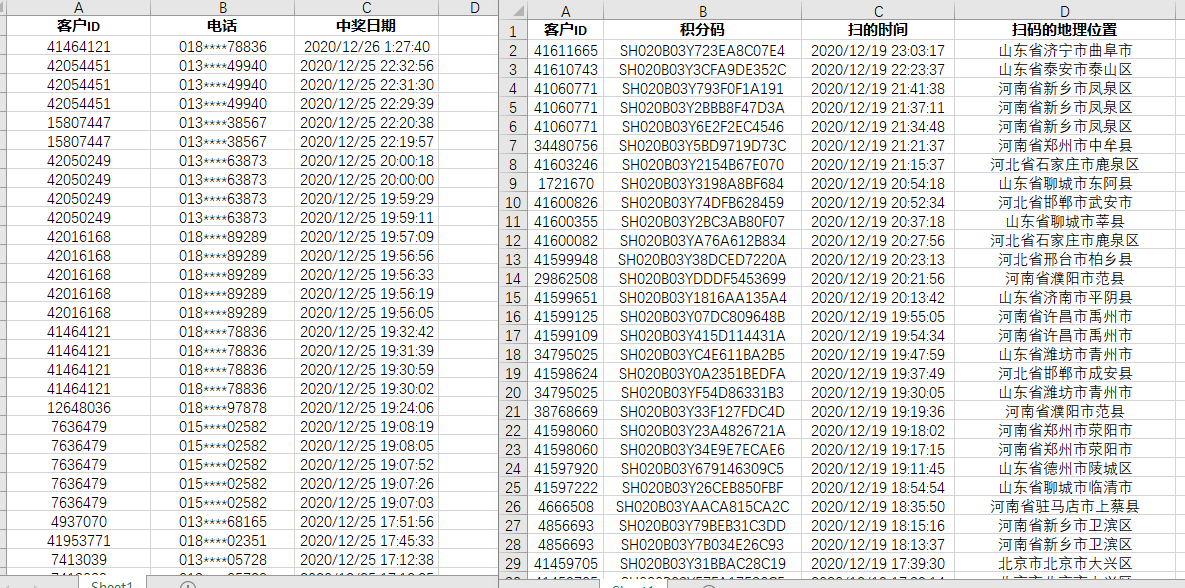
\includegraphics{picture/datetime/p1.png}
\caption{数据源视图}
\end{figure}

由于中奖时间和扫码时间不完全一致,导致没办法直接通过\texttt{客户ID}以及\texttt{时间}关联匹配找到客户每次中奖时的积分码,现在要求找到客户每次中奖时对应的积分码?

思路:通过观察数据,发现扫码后如果中奖,一般几秒钟内会有中奖记录,那我们就可以通过``每次中奖时间最近的一次扫码时间的积分码''就是该次中奖对应的积分码解决问题。这样我们通过简单编写自定义函数即可获取答案,即一个时间点从一串时间中找到离自己最近时间点。

\begin{Shaded}
\begin{Highlighting}[]
\NormalTok{testfun }\OtherTok{\textless{}{-}} \ControlFlowTok{function}\NormalTok{(x,y)\{}
\NormalTok{  result }\OtherTok{\textless{}{-}} \FunctionTok{data.frame}\NormalTok{() }\CommentTok{\#应采用列表存储结果向量化}
\NormalTok{  n  }\OtherTok{\textless{}{-}}  \FunctionTok{length}\NormalTok{(x)}
  \ControlFlowTok{for}\NormalTok{( i }\ControlFlowTok{in} \DecValTok{1}\SpecialCharTok{:}\NormalTok{n)\{}
\NormalTok{    res }\OtherTok{\textless{}{-}}\NormalTok{ x[i]}\SpecialCharTok{{-}}\NormalTok{y}
\NormalTok{    res }\OtherTok{\textless{}{-}} \FunctionTok{abs}\NormalTok{(res) }\SpecialCharTok{\%\textgreater{}\%} \FunctionTok{which.min}\NormalTok{() }\CommentTok{\#本处不对,应该判断res大于0的部分中谁最小}
\NormalTok{    kong }\OtherTok{\textless{}{-}} \FunctionTok{data.frame}\NormalTok{(中奖时间 }\OtherTok{=}\NormalTok{ x[i],扫的时间 }\OtherTok{=}\NormalTok{ y[res])}
\NormalTok{    result }\OtherTok{\textless{}{-}} \FunctionTok{rbind}\NormalTok{(kong,result)}
    
\NormalTok{  \}}
  \FunctionTok{return}\NormalTok{(result)}
\NormalTok{\}}
\NormalTok{res }\OtherTok{\textless{}{-}} \FunctionTok{testfun}\NormalTok{(dt}\SpecialCharTok{$}\NormalTok{时间,scan\_dt}\SpecialCharTok{$}\NormalTok{时间)}
\end{Highlighting}
\end{Shaded}

改进代码

\begin{Shaded}
\begin{Highlighting}[]
\NormalTok{testfun }\OtherTok{\textless{}{-}} \ControlFlowTok{function}\NormalTok{(x,y)\{}
\NormalTok{  n  }\OtherTok{\textless{}{-}}  \FunctionTok{length}\NormalTok{(x)}
\NormalTok{  result }\OtherTok{\textless{}{-}} \FunctionTok{list}\NormalTok{()}
  
  \ControlFlowTok{for}\NormalTok{( i }\ControlFlowTok{in} \DecValTok{1}\SpecialCharTok{:}\NormalTok{n)\{}
\NormalTok{    y }\OtherTok{\textless{}{-}}\NormalTok{ y[x}\SpecialCharTok{\textgreater{}}\NormalTok{y]}
\NormalTok{    res }\OtherTok{\textless{}{-}}\NormalTok{ x[i]}\SpecialCharTok{{-}}\NormalTok{y}
\NormalTok{    res }\OtherTok{\textless{}{-}}\NormalTok{ res }\SpecialCharTok{\%\textgreater{}\%} \FunctionTok{which.min}\NormalTok{() }
\NormalTok{    kong }\OtherTok{\textless{}{-}} \FunctionTok{data.frame}\NormalTok{(中奖时间 }\OtherTok{=}\NormalTok{ x[i],扫的时间 }\OtherTok{=}\NormalTok{ y[res])}
\NormalTok{    result[[i]] }\OtherTok{\textless{}{-}}\NormalTok{ kong}
\NormalTok{  \}}
  \FunctionTok{return}\NormalTok{(result)}
\NormalTok{\}}

\NormalTok{res }\OtherTok{\textless{}{-}} \FunctionTok{testfun}\NormalTok{(dt}\SpecialCharTok{$}\NormalTok{时间,scan\_dt}\SpecialCharTok{$}\NormalTok{时间)}
\end{Highlighting}
\end{Shaded}

理论上不同用户可以在同一时间扫码且同时中奖,那上面的代码即不可以获取正确答案。但是我们只要通过按照用户ID切割数据框后稍微改造上面的自定义函数即可。

\begin{Shaded}
\begin{Highlighting}[]
\NormalTok{testfun }\OtherTok{\textless{}{-}} \ControlFlowTok{function}\NormalTok{(dt)\{}
  
\NormalTok{  x }\OtherTok{\textless{}{-}}\NormalTok{ dt}\SpecialCharTok{$}\NormalTok{中奖时间}
\NormalTok{  y }\OtherTok{\textless{}{-}}\NormalTok{ dt}\SpecialCharTok{$}\NormalTok{扫的时间}
\NormalTok{  n  }\OtherTok{\textless{}{-}}  \FunctionTok{length}\NormalTok{(x)}
\NormalTok{  result }\OtherTok{\textless{}{-}} \FunctionTok{list}\NormalTok{()}
  
  \ControlFlowTok{for}\NormalTok{( i }\ControlFlowTok{in} \DecValTok{1}\SpecialCharTok{:}\NormalTok{n)\{}
\NormalTok{    y }\OtherTok{\textless{}{-}}\NormalTok{ y[x}\SpecialCharTok{\textgreater{}}\NormalTok{y]}
\NormalTok{    res }\OtherTok{\textless{}{-}}\NormalTok{ x[i]}\SpecialCharTok{{-}}\NormalTok{y}
\NormalTok{    res }\OtherTok{\textless{}{-}}\NormalTok{ res }\SpecialCharTok{\%\textgreater{}\%} \FunctionTok{which.min}\NormalTok{() }
\NormalTok{    kong }\OtherTok{\textless{}{-}} \FunctionTok{data.frame}\NormalTok{(中奖时间 }\OtherTok{=}\NormalTok{ x[i],扫的时间 }\OtherTok{=}\NormalTok{ y[res])}
\NormalTok{    result[[i]] }\OtherTok{\textless{}{-}}\NormalTok{ kong}
\NormalTok{  \}}
\NormalTok{  result }\OtherTok{\textless{}{-}}\NormalTok{ dplyr}\SpecialCharTok{::}\FunctionTok{bind\_rows}\NormalTok{(result)}
  \FunctionTok{return}\NormalTok{(result)}
\NormalTok{\}}
\NormalTok{dtlist }\OtherTok{\textless{}{-}} \FunctionTok{split}\NormalTok{(alldt,}\StringTok{\textquotesingle{}客户ID\textquotesingle{}}\NormalTok{)}
\NormalTok{purrr}\SpecialCharTok{::}\FunctionTok{map\_dfr}\NormalTok{(dtlist,testfun)}
\end{Highlighting}
\end{Shaded}

虽然可以通过寻找最近一次的扫码记录判断积分码,但是因为网络延迟或中途接电话等各种原因导致扫码时间和中奖时间相差并不是几秒,导致情景复杂,那我们就应该在设计系统时就设计好锁定对应关系,从根本上解决问题。

\hypertarget{ux8d44ux6599}{%
\section{资料}\label{ux8d44ux6599}}

\begin{itemize}
\item
  \url{https://cran.r-project.org/web/packages/lubridate/vignettes/lubridate.html}
\item
  \url{https://www.rdocumentation.org/packages/lubridate/versions/1.7.8}
\item
  pdf 下载 \url{https://rawgit.com/rstudio/cheatsheets/master/lubridate.pdf}
\item
  Excle中dax时间智能函数 \url{https://docs.microsoft.com/en-us/dax/time-intelligence-functions-dax}
\end{itemize}

\hypertarget{forcats}{%
\chapter{forcats}\label{forcats}}

我在实际工作中因子数据类型使用较少,forcats软件包用来处理因子,该软件包是tidyverse的一部分.

因子是用于对数据进行分类的R的一种数据类型. 它们可以存储字符串和整数.它们在具有有限数量的唯一值的列中很有用. 像``男性'',``女性''和True,False等。它们在统计建模的数据分析中很有用.

因子变量会占用更小空间,R4.0改变了字符默认为因子的方式.想了解更多请参考 \url{https://r4ds.had.co.nz/factors.html}

\begin{Shaded}
\begin{Highlighting}[]
\FunctionTok{object.size}\NormalTok{(}\FunctionTok{rep}\NormalTok{(letters,}\DecValTok{100000}\NormalTok{))}
\FunctionTok{object.size}\NormalTok{(}\FunctionTok{rep}\NormalTok{(forcats}\SpecialCharTok{::}\FunctionTok{as\_factor}\NormalTok{(letters),}\DecValTok{100000}\NormalTok{))}
\end{Highlighting}
\end{Shaded}

\hypertarget{ux521bux5efaux56e0ux5b50}{%
\section{创建因子}\label{ux521bux5efaux56e0ux5b50}}

实际工作中,可能各个事业部或部门之间没有实际顺序,但是在数据处理过程中需要指定顺序可以用因子.

\begin{Shaded}
\begin{Highlighting}[]
\FunctionTok{library}\NormalTok{(forcats)}
\NormalTok{vec1 }\OtherTok{\textless{}{-}} \FunctionTok{c}\NormalTok{(}\StringTok{\textquotesingle{}部门a\textquotesingle{}}\NormalTok{,}\StringTok{\textquotesingle{}部门b\textquotesingle{}}\NormalTok{,}\StringTok{\textquotesingle{}部门d\textquotesingle{}}\NormalTok{,}\StringTok{\textquotesingle{}部门f\textquotesingle{}}\NormalTok{)}
\FunctionTok{sort}\NormalTok{(vec1)}
\NormalTok{vec2 }\OtherTok{\textless{}{-}} \FunctionTok{as\_factor}\NormalTok{(}\FunctionTok{c}\NormalTok{(}\StringTok{\textquotesingle{}部门f\textquotesingle{}}\NormalTok{,}\StringTok{\textquotesingle{}部门d\textquotesingle{}}\NormalTok{,}\StringTok{\textquotesingle{}部门a\textquotesingle{}}\NormalTok{,}\StringTok{\textquotesingle{}部门b\textquotesingle{}}\NormalTok{))}
\FunctionTok{sort}\NormalTok{(vec2)}
\end{Highlighting}
\end{Shaded}

如上所示:实际工作中可以通过指定因子水平从而达到排序效果,在可视化中也可以运用,像指定X轴的顺序.

\hypertarget{data.table}{%
\chapter{data.table}\label{data.table}}

data.table包是我数据处理最常用的R包,是我目前觉得最好用的数据处理包,大部分我需要用到的功能集成在包里,不需要很多的依赖包。我简单接触过python,julia两种语言,并没有深入比较,所以我这个好用的印象仅仅是个人感受。

data.table包是我用了较长一段时间tidyverse系列后发现的``数据处理包''。已经忘记最初是什么吸引了我,我猜测可能是``大数据处理利器''之类的标签吸引了我,因为我喜欢``快''。但是和大部分人可能不同的是,初次接触时,语法的``怪异''并没有给我带来多少麻烦,因为我本来就没有编程基础以及很深的R语言基础。

所以我死记硬背data.table里一些常用用法,尤其喜欢拿Excle的一些用法参照,去实现Excle上面的部分操作,从读取、增、改、删除、筛选、计算列等常规操作入手。慢慢熟悉data.table语法之后,将会享受data.table带来的便利,其简洁的语法以及高效的计算速度(相比tidyverse系列)。

另外,Python中也有该包,目前正在积极开发中,期待ing,毕竟python也是很好用,在不同需求下选择不同的语言实现功能。

官方关于data.table的基础介绍请参阅:

\url{https://cran.r-project.org/web/packages/data.table/vignettes/datatable-intro.html}

data.table 优势:

\begin{itemize}
\tightlist
\item
  速度快
\item
  内存效率高
\item
  API生命周期管理好
\item
  语法简洁
\end{itemize}

\hypertarget{ux57faux7840ux4ecbux7ecd}{%
\section{基础介绍}\label{ux57faux7840ux4ecbux7ecd}}

本部分从data.table安装,内置的案例查看,到data.table的句式语法,实现基础行列筛选和聚合计算。

1.安装

安装详细信息请参考\href{https://github.com/Rdatatable/data.table/wiki/Installation}{the Installation wiki},有关于不同系统安装首次以及相关说明。

\begin{Shaded}
\begin{Highlighting}[]
\FunctionTok{install.packages}\NormalTok{(}\StringTok{"data.table"}\NormalTok{)}
\CommentTok{\# latest development version:}
\NormalTok{data.table}\SpecialCharTok{::}\FunctionTok{update.dev.pkg}\NormalTok{()}
\end{Highlighting}
\end{Shaded}

2.使用说明

通过以下代码查看内置的使用案例。

\begin{Shaded}
\begin{Highlighting}[]
\FunctionTok{library}\NormalTok{(data.table)}
\FunctionTok{example}\NormalTok{(data.table)}
\end{Highlighting}
\end{Shaded}

\hypertarget{ux8bfbux53d6ux6570ux636e}{%
\subsection{读取数据}\label{ux8bfbux53d6ux6570ux636e}}

在我实际工作中接触的数据大部分以数据库,csv,Excel等形式存在,并且CSV格式数据较少。但是data.table包读取数据的\texttt{fread}函数仅接受CSV格式。如果是Excel格式文件,需要通过如\texttt{readxl},\texttt{openxlsx}等包读入后转换为\texttt{data.table}格式数据。

fread 函数可以直接读取CSV格式文件,无论是本地文件或者在线文件.

本文会照搬很多官方关于data.table的demo.

\begin{Shaded}
\begin{Highlighting}[]
\FunctionTok{library}\NormalTok{(data.table)}
\NormalTok{input }\OtherTok{\textless{}{-}} \ControlFlowTok{if}\NormalTok{ (}\FunctionTok{file.exists}\NormalTok{(}\StringTok{"./data/flights.csv"}\NormalTok{)) \{}
   \StringTok{"./data/flights.csv"} \CommentTok{\#本地文件}
\NormalTok{\} }\ControlFlowTok{else}\NormalTok{ \{}
  \StringTok{"https://raw.githubusercontent.com/Rdatatable/data.table/master/vignettes/flights.csv"} \CommentTok{\#在线文件需翻墙}
\NormalTok{\}}
\NormalTok{flights }\OtherTok{\textless{}{-}} \FunctionTok{fread}\NormalTok{(input) }\CommentTok{\#具体参数请参照文档  实际工作中可能会用到的encoding参数,编码 encoding=\textquotesingle{}UTF{-}8\textquotesingle{}}

\FunctionTok{head}\NormalTok{(flights)}
\end{Highlighting}
\end{Shaded}

本文读取本地文件,如果该数据集下载失败,可更改地址为(\url{http://www.zhongyufei.com/datatable/data/flights.csv})

\begin{Shaded}
\begin{Highlighting}[]
\NormalTok{flights }\OtherTok{\textless{}{-}} \FunctionTok{fread}\NormalTok{(}\StringTok{"http://www.zhongyufei.com/datatable/data/flights.csv"}\NormalTok{)}
\end{Highlighting}
\end{Shaded}

数据集记录的是 2014 年,纽约市3大机场(分别为:JFK 肯尼迪国际机场、 LGA 拉瓜迪亚机场,和 EWR 纽瓦克自由国际机场)起飞的航班信息。

具体的记录信息(特征列),包括起飞时间、到达时间、延误时长、航空公司、始发机场、目的机场、飞行时长,和飞行距离等。

\hypertarget{ux57faux672cux683cux5f0f}{%
\subsection{基本格式}\label{ux57faux672cux683cux5f0f}}

\texttt{DT{[}i,\ j,\ by{]}}是data.table的基本样式,在不同位置上实现不同功能。

\begin{figure}
\centering
\includegraphics{https://gitee.com/zhongyufei/photo-bed/raw/pic/img/data.table-i-j-by\%E4\%BB\%8B\%E7\%BB\%8D.png}
\caption{i-j-by}
\end{figure}

\begin{Shaded}
\begin{Highlighting}[]
\NormalTok{DT[i, j, by]}
\DocumentationTok{\#\#   R:                 i                 j        by}
\DocumentationTok{\#\# SQL:  where | order by   select | update  group by}
\end{Highlighting}
\end{Shaded}

data.table个人理解主要有三大类参数,i参数做筛选,j参数做计算,by参数做分组.

拿Excel透视表类别,i位置参数当作『筛选』,by位置用来做汇总字段『行』,j位置当作『值』,如下所示:

\begin{figure}
\centering
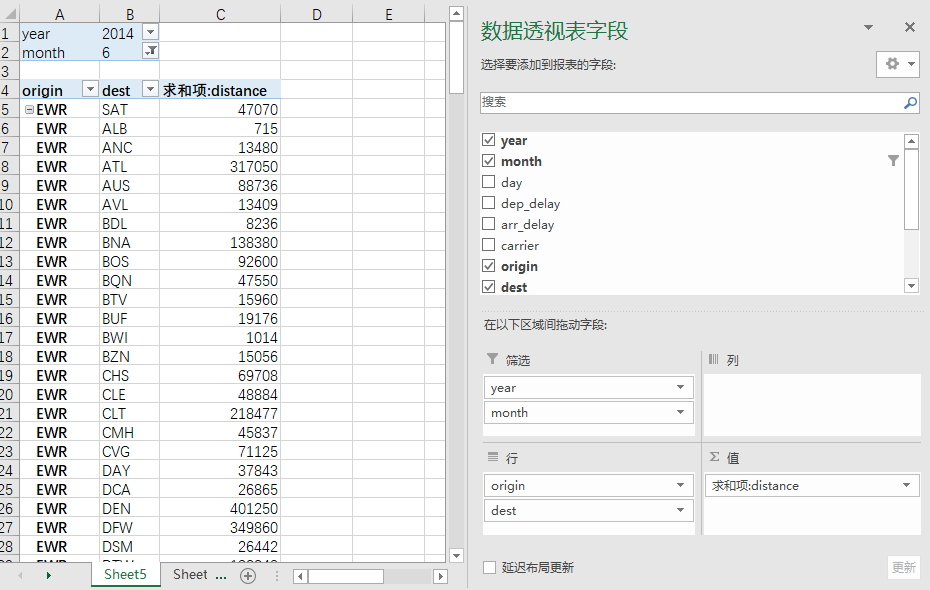
\includegraphics{./picture/data-table/01picture.png}
\caption{透视表截图}
\end{figure}

1.代码实例

代码求2014年6月,从各始发机场到各目的机场的飞行距离求和.

\begin{Shaded}
\begin{Highlighting}[]
\FunctionTok{library}\NormalTok{(data.table)}
\NormalTok{flights }\OtherTok{\textless{}{-}} \FunctionTok{fread}\NormalTok{(}\StringTok{"./data/flights.csv"}\NormalTok{)}
\NormalTok{flights[year}\SpecialCharTok{==}\DecValTok{2014} \SpecialCharTok{\&}\NormalTok{ month}\SpecialCharTok{==}\DecValTok{6}\NormalTok{,.(求和项}\AttributeTok{distance=}\FunctionTok{sum}\NormalTok{(distance)),by}\OtherTok{=}\NormalTok{.(origin,dest)]}
\end{Highlighting}
\end{Shaded}

2.代码解释

i 的部分:条件year==2014 和 month==6 ;

j 的部分:求和项distance=sum(distance),写在.()中或者list()中;

by 的部分.(origin,dest),重点是写在.()中,和Excel透视表一一对应。

至于为什么要用.()包裹起来,最开始默认为格式强制要求。就这个问题我想说:大部分人可能觉得是比较``怪异''的用法,并且不理解,从而可能留下data.table不好用,很古怪的印象,但是我觉得任何东西存在即合理,你学一个东西总得接受一些你可能不认可的东西,这样可能才是真正的学习,就像拿Python来做数据分析,我刚开始觉得pandas很难用,很反人类,但是后来知道python代码可以直接打包封装成exe后,觉得真香,说这么多主要是想表达我们学会挑选合适的工具用,适应它,用好它就可以了。

\hypertarget{i-j-by-ux4f7fux7528}{%
\subsection{i j by 使用}\label{i-j-by-ux4f7fux7528}}

使用data.table处理数据,接下来我们就用该函数读取数据演示i,j,by的简单使用。

\hypertarget{iux884cux7b5bux9009}{%
\subsubsection{i行筛选}\label{iux884cux7b5bux9009}}

行筛选是一种很常见的数据操作行为,类似我们Excel中的筛选,即按照一定条件筛选符合要求的数据。条件筛选一般分为单条件筛选、多条件筛选;

在筛选时涉及到条件判断,R语言中常用的条件判断分为逻辑运算、关系运算。常用的关系运算符 \textgreater、 \textless、==、!=、\textgreater=、\textless=分别代表大于、小于、等于、不等于、大于等于、小于等于。常用的逻辑运算符 \&、\textbar、!等。

\begin{Shaded}
\begin{Highlighting}[]
\CommentTok{\#单条件筛选}
\NormalTok{filghts[year }\SpecialCharTok{==} \DecValTok{2014}\NormalTok{] }\CommentTok{\#筛选year==2014}
\CommentTok{\#多条件筛选 用 \& 链接}
\NormalTok{flights[ year }\SpecialCharTok{==} \DecValTok{2014} \SpecialCharTok{\&}\NormalTok{ month }\SpecialCharTok{==} \DecValTok{6}\NormalTok{] }
\CommentTok{\# | 相当于中文条件或 }
\NormalTok{flights[ month }\SpecialCharTok{==} \DecValTok{5} \SpecialCharTok{|}\NormalTok{ month }\SpecialCharTok{==} \DecValTok{6}\NormalTok{] }
\CommentTok{\# \%in\% 类似sql中in用法}
\NormalTok{flights[month }\SpecialCharTok{\%in\%} \FunctionTok{c}\NormalTok{(}\DecValTok{1}\NormalTok{,}\DecValTok{3}\NormalTok{,}\DecValTok{5}\NormalTok{,}\DecValTok{7}\NormalTok{,}\DecValTok{9}\NormalTok{)] }
\CommentTok{\# \%between\% 类似sql中between and 用法}
\NormalTok{flights[month }\SpecialCharTok{\%between\%} \FunctionTok{c}\NormalTok{(}\DecValTok{1}\NormalTok{,}\DecValTok{7}\NormalTok{)]}
\end{Highlighting}
\end{Shaded}

\hypertarget{jux5217ux64cdux4f5c}{%
\subsubsection{j列操作}\label{jux5217ux64cdux4f5c}}

数据集较大、字段较多时,由于无效信息较多可以做适当精选,这时需要我们筛选列。与sql中的select用法一致,即保留想要的字段。

.()或list()是data.table中的比较特殊的实现列筛选的用法。常规数字索引,字符向量索引同样有效。

\begin{Shaded}
\begin{Highlighting}[]
\CommentTok{\#注意前面的. .()}
\NormalTok{flights[,.(year,month,day,dep\_delay,carrier,origin)] }
\CommentTok{\# flights[,list(year,month,day,dep\_delay,carrier,origin)]  same above}

\CommentTok{\# not run}
\CommentTok{\# flights[,1:3]}

\CommentTok{\# not run}
\CommentTok{\# flights[,c(\textquotesingle{}year\textquotesingle{},\textquotesingle{}month\textquotesingle{},\textquotesingle{}day\textquotesingle{})]}
\end{Highlighting}
\end{Shaded}

setcolorder函数可以调整列的顺序,将常用的字段信息排在前面可以用过该函数实现。

\begin{Shaded}
\begin{Highlighting}[]
\CommentTok{\# not run}
\CommentTok{\# setcolorder(x = flights,neworder = c( "month","day","dep\_delay" ,"arr\_delay","carrier" )) }
\CommentTok{\# 按照指定列顺序排序 其余字段保持不变,不是建立副本,是直接修改了flights 数据的列顺序}
\end{Highlighting}
\end{Shaded}

\begin{itemize}
\tightlist
\item
  常规计算
\end{itemize}

根据最开始的Excel透视表截图,我们想要获得如截图一样的结果该怎么实现呢?代码如下:

\begin{Shaded}
\begin{Highlighting}[]
\NormalTok{flights[year}\SpecialCharTok{==}\DecValTok{2014} \SpecialCharTok{\&}\NormalTok{ month}\SpecialCharTok{==}\DecValTok{6}\NormalTok{,.(求和项}\AttributeTok{distance=}\FunctionTok{sum}\NormalTok{(distance),平均距离}\OtherTok{=}\FunctionTok{mean}\NormalTok{(distance)),by}\OtherTok{=}\NormalTok{.(origin,dest)]}
\end{Highlighting}
\end{Shaded}

在i的位置做筛选,j的位置做计算,by指定分组字段。在j的位置可以做各种各样的计算,R中自带的函数,或者是自己定义的函数。

\begin{Shaded}
\begin{Highlighting}[]
\NormalTok{myfun }\OtherTok{\textless{}{-}} \ControlFlowTok{function}\NormalTok{(x)\{}
\NormalTok{    x}\SpecialCharTok{\^{}}\DecValTok{2}\SpecialCharTok{/}\DecValTok{2}
\NormalTok{\}}
\NormalTok{flights[year}\SpecialCharTok{==}\DecValTok{2014} \SpecialCharTok{\&}\NormalTok{ month}\SpecialCharTok{==}\DecValTok{6}\NormalTok{,.(}\FunctionTok{myfun}\NormalTok{(distance)),by}\OtherTok{=}\NormalTok{.(origin,dest)]}
\end{Highlighting}
\end{Shaded}

\hypertarget{by-ux5206ux7ec4}{%
\subsubsection{by 分组}\label{by-ux5206ux7ec4}}

分组是按照某种分组实现一定条件下某种聚合方式的计算。分组可以是单字段,多字段以及条件字段等。

1.按月分组

\begin{Shaded}
\begin{Highlighting}[]
\NormalTok{flights[,.(}\FunctionTok{sum}\NormalTok{(distance)),by}\OtherTok{=}\NormalTok{.(month)]}
\end{Highlighting}
\end{Shaded}

2.多条件分组

\begin{Shaded}
\begin{Highlighting}[]
\NormalTok{dt }\OtherTok{\textless{}{-}}\NormalTok{ flights[,.(}\FunctionTok{sum}\NormalTok{(distance)),by}\OtherTok{=}\NormalTok{.(carrier,origin)]}
\FunctionTok{head}\NormalTok{(dt)}
\CommentTok{\#可直接重新命名}
\NormalTok{dt }\OtherTok{\textless{}{-}}\NormalTok{ flights[,.(}\FunctionTok{sum}\NormalTok{(distance)),by}\OtherTok{=}\NormalTok{.(}\AttributeTok{newcol1 =}\NormalTok{ carrier,}\AttributeTok{newcol2 =}\NormalTok{ origin)]}
\FunctionTok{head}\NormalTok{(dt)}
\end{Highlighting}
\end{Shaded}

3.按月份是否大于6分组

即得到是否大于6的两类分组

\begin{Shaded}
\begin{Highlighting}[]
\NormalTok{dt }\OtherTok{\textless{}{-}}\NormalTok{ flights[,.(}\FunctionTok{sum}\NormalTok{(distance)),by}\OtherTok{=}\NormalTok{.(month}\SpecialCharTok{\textgreater{}}\DecValTok{6}\NormalTok{)] }\CommentTok{\#by里面可以做计算}
\FunctionTok{head}\NormalTok{(dt)}
\end{Highlighting}
\end{Shaded}

\hypertarget{ux884cux5217ux7b5bux9009ux603bux7ed3}{%
\subsection{行列筛选总结}\label{ux884cux5217ux7b5bux9009ux603bux7ed3}}

行筛选在 i 的位置上进行, 列筛选在 j 的位置上进行;data.table中j的位置比较灵活多变,但是i的位置大部分时候都是进行条件筛选。我们通过上述的行列筛选已经大概知道data.table中i,j的用法。也就是我们常规数据清洗过程中的数据筛选过程,筛选符合要求的数据记录。

\begin{Shaded}
\begin{Highlighting}[]

\NormalTok{dt }\OtherTok{\textless{}{-}}\NormalTok{ flights[ year }\SpecialCharTok{==} \DecValTok{2014} \SpecialCharTok{\&}\NormalTok{ month }\SpecialCharTok{==} \DecValTok{6} \SpecialCharTok{\&}\NormalTok{ day }\SpecialCharTok{\textgreater{}=}\DecValTok{15}\NormalTok{,.(year,month,day,dep\_delay,carrier,origin)] }
\FunctionTok{head}\NormalTok{(dt)}
\end{Highlighting}
\end{Shaded}

\hypertarget{ux5e38ux89c4ux64cdux4f5c}{%
\section{常规操作}\label{ux5e38ux89c4ux64cdux4f5c}}

\hypertarget{ux884cux7b5bux9009}{%
\subsection{行筛选}\label{ux884cux7b5bux9009}}

上文已经大致讲过行筛选,但是行筛选使用有一定的技巧,涉及到运算的快慢。主要是逻辑条件的设置,交集并集之间的差异。除了上文中的关系运算筛选,逻辑运算筛选除外,data.table中还有几个常用的筛选函数。

\begin{itemize}
\tightlist
\item
  数字向量筛选
\end{itemize}

\%in\%用法与 sql 中 in 用法类似。

\begin{Shaded}
\begin{Highlighting}[]
\CommentTok{\# 筛选 \%in\% }
\NormalTok{flights[ hour }\SpecialCharTok{\%in\%} \FunctionTok{seq}\NormalTok{(}\DecValTok{1}\NormalTok{,}\DecValTok{24}\NormalTok{,}\DecValTok{2}\NormalTok{) ]}
\end{Highlighting}
\end{Shaded}

\begin{itemize}
\tightlist
\item
  字符向量筛选
\end{itemize}

\%chin\%用法与 \%in\% 类似,但仅仅针对字符。

\begin{Shaded}
\begin{Highlighting}[]
\CommentTok{\# 字符筛选}
\NormalTok{flights[ origin }\SpecialCharTok{\%chin\%} \FunctionTok{c}\NormalTok{(}\StringTok{\textquotesingle{}JFK\textquotesingle{}}\NormalTok{,}\StringTok{\textquotesingle{}LGA\textquotesingle{}}\NormalTok{)]}
\CommentTok{\# not run 同上 \%chin\% 对字符速度筛选速度更快}
\CommentTok{\#flights[ origin \%in\% c(\textquotesingle{}JFK\textquotesingle{},\textquotesingle{}LGA\textquotesingle{})]}
\end{Highlighting}
\end{Shaded}

\begin{itemize}
\tightlist
\item
  between 筛选
\end{itemize}

该函数的新特性矢量化挺实用。

\begin{Shaded}
\begin{Highlighting}[]
\CommentTok{\#between 函数参数}
\CommentTok{\#between(x, lower, upper, incbounds=TRUE, NAbounds=TRUE, check=FALSE)}
\NormalTok{X }\OtherTok{\textless{}{-}}  \FunctionTok{data.table}\NormalTok{(}\AttributeTok{a=}\DecValTok{1}\SpecialCharTok{:}\DecValTok{5}\NormalTok{, }\AttributeTok{b=}\DecValTok{6}\SpecialCharTok{:}\DecValTok{10}\NormalTok{, }\AttributeTok{c=}\FunctionTok{c}\NormalTok{(}\DecValTok{5}\SpecialCharTok{:}\DecValTok{1}\NormalTok{))}
\NormalTok{X[b }\SpecialCharTok{\%between\%} \FunctionTok{c}\NormalTok{(}\DecValTok{7}\NormalTok{,}\DecValTok{9}\NormalTok{)]}
\NormalTok{X[}\FunctionTok{between}\NormalTok{(b, }\DecValTok{7}\NormalTok{, }\DecValTok{9}\NormalTok{)] }\CommentTok{\#效果同上}
\NormalTok{X[c }\SpecialCharTok{\%between\%} \FunctionTok{list}\NormalTok{(a,b)] }\CommentTok{\# 矢量化}
\end{Highlighting}
\end{Shaded}

\begin{itemize}
\tightlist
\item
  like 筛选
\end{itemize}

\%like\% 用法与SQL中 like 类似。

\begin{Shaded}
\begin{Highlighting}[]
\CommentTok{\# \%like\% 用法与SQL中 like 类似}
\NormalTok{DT }\OtherTok{=} \FunctionTok{data.table}\NormalTok{(}\AttributeTok{Name=}\FunctionTok{c}\NormalTok{(}\StringTok{"Mary"}\NormalTok{,}\StringTok{"George"}\NormalTok{,}\StringTok{"Martha"}\NormalTok{), }\AttributeTok{Salary=}\FunctionTok{c}\NormalTok{(}\DecValTok{2}\NormalTok{,}\DecValTok{3}\NormalTok{,}\DecValTok{4}\NormalTok{))}
\NormalTok{DT[Name }\SpecialCharTok{\%like\%} \StringTok{"\^{}Mar"}\NormalTok{]}
\end{Highlighting}
\end{Shaded}

\hypertarget{ux65b0ux589eux66f4ux65b0ux5217}{%
\subsection{新增更新列}\label{ux65b0ux589eux66f4ux65b0ux5217}}

新增或删除或更新列是我们数据清洗过程中的常规操作,\texttt{data.table中}实现该类功能是通过\texttt{:=}符号实现。

\begin{itemize}
\tightlist
\item
  选择列
\end{itemize}

\begin{Shaded}
\begin{Highlighting}[]
\NormalTok{dt }\OtherTok{\textless{}{-}} \FunctionTok{data.table}\NormalTok{(}\AttributeTok{col1=}\DecValTok{1}\SpecialCharTok{:}\DecValTok{10}\NormalTok{,}\AttributeTok{col2=}\NormalTok{letters[}\DecValTok{1}\SpecialCharTok{:}\DecValTok{10}\NormalTok{],}\AttributeTok{col3=}\NormalTok{LETTERS[}\DecValTok{1}\SpecialCharTok{:}\DecValTok{10}\NormalTok{],}\AttributeTok{col4=}\DecValTok{1}\SpecialCharTok{:}\DecValTok{10}\NormalTok{)}
\NormalTok{dt[,.(col1,col2)]}
\CommentTok{\# same above}
\NormalTok{dt[,}\FunctionTok{list}\NormalTok{(col1,col2)]}
\end{Highlighting}
\end{Shaded}

\begin{itemize}
\tightlist
\item
  新增列
\end{itemize}

如下所示:新增addcol列,最后的{[}{]}是为了显示新增列的数据框,可不增加。

\begin{Shaded}
\begin{Highlighting}[]
\CommentTok{\#data.table()函数创建data.table数据框}
\NormalTok{dt }\OtherTok{\textless{}{-}} \FunctionTok{data.table}\NormalTok{(}\AttributeTok{col1=}\DecValTok{1}\SpecialCharTok{:}\DecValTok{10}\NormalTok{,}\AttributeTok{col2=}\NormalTok{letters[}\DecValTok{1}\SpecialCharTok{:}\DecValTok{10}\NormalTok{],}\AttributeTok{col3=}\NormalTok{LETTERS[}\DecValTok{1}\SpecialCharTok{:}\DecValTok{10}\NormalTok{],}\AttributeTok{col4=}\DecValTok{1}\SpecialCharTok{:}\DecValTok{10}\NormalTok{)}
\CommentTok{\# 新增列 :=}
\NormalTok{dt[,addcol}\SpecialCharTok{:}\ErrorTok{=}\FunctionTok{rep}\NormalTok{(}\StringTok{\textquotesingle{}新列\textquotesingle{}}\NormalTok{,}\DecValTok{10}\NormalTok{)][] }\CommentTok{\#最后的[]是为了显示新增列的数据框,可不增加}
\CommentTok{\#dt[,addcol:=rep(\textquotesingle{}新列\textquotesingle{},10)] 不会显示返回结果,加上[]会显示返回}
\CommentTok{\# 新增多列}
\NormalTok{dt[,}\StringTok{\textasciigrave{}}\AttributeTok{:=}\StringTok{\textasciigrave{}}\NormalTok{(}\AttributeTok{newcol1=}\FunctionTok{rep}\NormalTok{(}\StringTok{\textquotesingle{}newcol1\textquotesingle{}}\NormalTok{,}\DecValTok{10}\NormalTok{),}\AttributeTok{newcol2=}\FunctionTok{rep}\NormalTok{(}\StringTok{\textquotesingle{}newcol2\textquotesingle{}}\NormalTok{,}\DecValTok{10}\NormalTok{))][]}
\end{Highlighting}
\end{Shaded}

\begin{itemize}
\tightlist
\item
  删除列
\end{itemize}

删除列即将列赋值NULL即可

\begin{Shaded}
\begin{Highlighting}[]
\CommentTok{\# 删除列}
\NormalTok{dt[,col1}\SpecialCharTok{:}\ErrorTok{=}\ConstantTok{NULL}\NormalTok{][]}
\CommentTok{\# 删除多列}
\NormalTok{dt[,}\FunctionTok{c}\NormalTok{(}\StringTok{\textquotesingle{}newcol1\textquotesingle{}}\NormalTok{,}\StringTok{\textquotesingle{}newcol2\textquotesingle{}}\NormalTok{)}\SpecialCharTok{:}\ErrorTok{=}\ConstantTok{NULL}\NormalTok{][]}
\end{Highlighting}
\end{Shaded}

\begin{itemize}
\tightlist
\item
  更新
\end{itemize}

更新即重新赋值,将现有列参与计算等于是重新赋值,可以看成是更新列。

\begin{Shaded}
\begin{Highlighting}[]
\CommentTok{\# 更新列}
\NormalTok{dt[,col1}\SpecialCharTok{:}\ErrorTok{=}\DecValTok{11}\SpecialCharTok{:}\DecValTok{20}\NormalTok{][]}
\CommentTok{\# not run }
\CommentTok{\# 两列间计算 也可以理解为更新}
\NormalTok{dt[,newcol}\SpecialCharTok{:}\ErrorTok{=}\NormalTok{col1}\SpecialCharTok{/}\NormalTok{col4]}
\end{Highlighting}
\end{Shaded}

\begin{quote}
Note: DT{[}a \textgreater{} 4, b := c{]} is different from DT{[}a \textgreater{} 4{]}{[}, b := c{]}
\end{quote}

\hypertarget{ux6392ux5e8f}{%
\subsection{排序}\label{ux6392ux5e8f}}

当我们清洗数据时,我们需要将数据框排序,我们可以使用\texttt{setorder}或\texttt{setorderv}函数实现排序。函数是\texttt{data.table}包的函数,比base R 中的\texttt{order}函数要节省内存。
注意:按照函数文档说法:Note that queries like x{[}order(.){]} are optimised internally to use data.table's fast order。即x{[}order(.){]}这样的用法会被优化为data.table的排序方法。

\begin{Shaded}
\begin{Highlighting}[]
\FunctionTok{set.seed}\NormalTok{(45L)}
\NormalTok{DT }\OtherTok{=} \FunctionTok{data.table}\NormalTok{(}\AttributeTok{A=}\FunctionTok{sample}\NormalTok{(}\DecValTok{3}\NormalTok{, }\DecValTok{10}\NormalTok{, }\ConstantTok{TRUE}\NormalTok{),}
         \AttributeTok{B=}\FunctionTok{sample}\NormalTok{(letters[}\DecValTok{1}\SpecialCharTok{:}\DecValTok{3}\NormalTok{], }\DecValTok{10}\NormalTok{, }\ConstantTok{TRUE}\NormalTok{), }\AttributeTok{C=}\FunctionTok{sample}\NormalTok{(}\DecValTok{10}\NormalTok{))}

\FunctionTok{setorder}\NormalTok{(DT, A, }\SpecialCharTok{{-}}\NormalTok{B) }\CommentTok{\#将DT按照A、B排序 A 升序,{-}B降序}

\CommentTok{\# 和上面同样的效果 但是函数变成 setorderv}
\FunctionTok{setorderv}\NormalTok{(DT, }\FunctionTok{c}\NormalTok{(}\StringTok{"A"}\NormalTok{, }\StringTok{"B"}\NormalTok{), }\FunctionTok{c}\NormalTok{(}\DecValTok{1}\NormalTok{, }\SpecialCharTok{{-}}\DecValTok{1}\NormalTok{))}
\end{Highlighting}
\end{Shaded}

\hypertarget{ux5e38ux7528ux51fdux6570-2}{%
\section{常用函数}\label{ux5e38ux7528ux51fdux6570-2}}

常用函数指我们常用功能的函数,如排名、排序、非重复计数、判断、表连接、长宽转换等功能。

\hypertarget{ux7279ux6b8aux7b26ux53f7}{%
\subsection{特殊符号}\label{ux7279ux6b8aux7b26ux53f7}}

.SD,.BY,.N,.I,.NGRP和.GRP,.SDcols等,只能用在 j 的位置,.N 可以用在 i 的位置。

如果想要记住用法需要自己多尝试练习,对于我来说.N使用较多。

\begin{Shaded}
\begin{Highlighting}[]
\NormalTok{DT }\OtherTok{=} \FunctionTok{data.table}\NormalTok{(}\AttributeTok{x=}\FunctionTok{rep}\NormalTok{(}\FunctionTok{c}\NormalTok{(}\StringTok{"b"}\NormalTok{,}\StringTok{"a"}\NormalTok{,}\StringTok{"c"}\NormalTok{),}\AttributeTok{each=}\DecValTok{3}\NormalTok{), }\AttributeTok{v=}\FunctionTok{c}\NormalTok{(}\DecValTok{1}\NormalTok{,}\DecValTok{1}\NormalTok{,}\DecValTok{1}\NormalTok{,}\DecValTok{2}\NormalTok{,}\DecValTok{2}\NormalTok{,}\DecValTok{1}\NormalTok{,}\DecValTok{1}\NormalTok{,}\DecValTok{2}\NormalTok{,}\DecValTok{2}\NormalTok{), }\AttributeTok{y=}\FunctionTok{c}\NormalTok{(}\DecValTok{1}\NormalTok{,}\DecValTok{3}\NormalTok{,}\DecValTok{6}\NormalTok{), }\AttributeTok{a=}\DecValTok{1}\SpecialCharTok{:}\DecValTok{9}\NormalTok{, }\AttributeTok{b=}\DecValTok{9}\SpecialCharTok{:}\DecValTok{1}\NormalTok{)}
\NormalTok{DT}
\NormalTok{X }\OtherTok{=} \FunctionTok{data.table}\NormalTok{(}\AttributeTok{x=}\FunctionTok{c}\NormalTok{(}\StringTok{"c"}\NormalTok{,}\StringTok{"b"}\NormalTok{), }\AttributeTok{v=}\DecValTok{8}\SpecialCharTok{:}\DecValTok{7}\NormalTok{, }\AttributeTok{foo=}\FunctionTok{c}\NormalTok{(}\DecValTok{4}\NormalTok{,}\DecValTok{2}\NormalTok{))}
\NormalTok{X}

\CommentTok{\# 用在i的位置}
\NormalTok{DT[.N] }\CommentTok{\#取DT最后一行,.N 计数函数}
\NormalTok{DT[,.N] }\CommentTok{\#DT 共有多少行记录 返回一个整数}
\NormalTok{DT[, .N, by}\OtherTok{=}\NormalTok{x]  }\CommentTok{\#分组计数}
\NormalTok{DT[, .SD, .SDcols}\OtherTok{=}\NormalTok{x}\SpecialCharTok{:}\NormalTok{y]  }\CommentTok{\# 选择x 到y 列}
\CommentTok{\#DT[, .SD, .SDcols=c("x","y")] 与上面不一样}

\NormalTok{DT[, .SD[}\DecValTok{1}\NormalTok{]] }\CommentTok{\#取第一行}
\NormalTok{DT[, .SD[}\DecValTok{1}\NormalTok{], by}\OtherTok{=}\NormalTok{x] }\CommentTok{\#按x列分组后}
\NormalTok{DT[, }\FunctionTok{c}\NormalTok{(.N, }\FunctionTok{lapply}\NormalTok{(.SD, sum)), by}\OtherTok{=}\NormalTok{x] }\CommentTok{\#按照x分组后 行数计数和每列求和}
\end{Highlighting}
\end{Shaded}

\hypertarget{ux6392ux5e8fux51fdux6570-1}{%
\subsection{排序函数}\label{ux6392ux5e8fux51fdux6570-1}}

\texttt{frank}和\texttt{frankv}函数参数如下:

\begin{Shaded}
\begin{Highlighting}[]
\FunctionTok{frank}\NormalTok{(x, ..., }\AttributeTok{na.last=}\ConstantTok{TRUE}\NormalTok{, }\AttributeTok{ties.method=}\FunctionTok{c}\NormalTok{(}\StringTok{"average"}\NormalTok{,}
  \StringTok{"first"}\NormalTok{, }\StringTok{"last"}\NormalTok{, }\StringTok{"random"}\NormalTok{, }\StringTok{"max"}\NormalTok{, }\StringTok{"min"}\NormalTok{, }\StringTok{"dense"}\NormalTok{))}

\FunctionTok{frankv}\NormalTok{(x, }\AttributeTok{cols=}\FunctionTok{seq\_along}\NormalTok{(x), }\AttributeTok{order=}\NormalTok{1L, }\AttributeTok{na.last=}\ConstantTok{TRUE}\NormalTok{,}
      \AttributeTok{ties.method=}\FunctionTok{c}\NormalTok{(}\StringTok{"average"}\NormalTok{, }\StringTok{"first"}\NormalTok{, }\StringTok{"random"}\NormalTok{,}
        \StringTok{"max"}\NormalTok{, }\StringTok{"min"}\NormalTok{, }\StringTok{"dense"}\NormalTok{))}
\end{Highlighting}
\end{Shaded}

官方案例,如下所示:

\begin{Shaded}
\begin{Highlighting}[]
\CommentTok{\# on vectors}
\NormalTok{x }\OtherTok{=} \FunctionTok{c}\NormalTok{(}\DecValTok{4}\NormalTok{, }\DecValTok{1}\NormalTok{, }\DecValTok{4}\NormalTok{, }\ConstantTok{NA}\NormalTok{, }\DecValTok{1}\NormalTok{, }\ConstantTok{NA}\NormalTok{, }\DecValTok{4}\NormalTok{)}
\CommentTok{\# NAs are considered identical (unlike base R)}
\CommentTok{\# default is average}
\FunctionTok{frankv}\NormalTok{(x) }\CommentTok{\# na.last=TRUE}
\FunctionTok{frankv}\NormalTok{(x, }\AttributeTok{na.last=}\ConstantTok{FALSE}\NormalTok{)}

\CommentTok{\# on data.table}
\NormalTok{DT }\OtherTok{=} \FunctionTok{data.table}\NormalTok{(x, }\AttributeTok{y=}\FunctionTok{c}\NormalTok{(}\DecValTok{1}\NormalTok{, }\DecValTok{1}\NormalTok{, }\DecValTok{1}\NormalTok{, }\DecValTok{0}\NormalTok{, }\ConstantTok{NA}\NormalTok{, }\DecValTok{0}\NormalTok{, }\DecValTok{2}\NormalTok{))}
\FunctionTok{frankv}\NormalTok{(DT, }\AttributeTok{cols=}\StringTok{"x"}\NormalTok{) }\CommentTok{\# same as frankv(x) from before}
\FunctionTok{frankv}\NormalTok{(DT, }\AttributeTok{cols=}\StringTok{"x"}\NormalTok{, }\AttributeTok{na.last=}\StringTok{"keep"}\NormalTok{)}
\FunctionTok{frankv}\NormalTok{(DT, }\AttributeTok{cols=}\StringTok{"x"}\NormalTok{, }\AttributeTok{ties.method=}\StringTok{"dense"}\NormalTok{, }\AttributeTok{na.last=}\ConstantTok{NA}\NormalTok{)}
\FunctionTok{frank}\NormalTok{(DT, x, }\AttributeTok{ties.method=}\StringTok{"dense"}\NormalTok{, }\AttributeTok{na.last=}\ConstantTok{NA}\NormalTok{) }\CommentTok{\# equivalent of above using frank}
\end{Highlighting}
\end{Shaded}

\begin{itemize}
\tightlist
\item
  frankv在排序时,NA被认为是一样的,基础base R 中认为不一样.
\end{itemize}

\begin{Shaded}
\begin{Highlighting}[]
\NormalTok{x }\OtherTok{\textless{}{-}}  \FunctionTok{c}\NormalTok{(}\DecValTok{4}\NormalTok{, }\DecValTok{1}\NormalTok{, }\DecValTok{4}\NormalTok{, }\ConstantTok{NA}\NormalTok{, }\DecValTok{1}\NormalTok{, }\ConstantTok{NA}\NormalTok{, }\DecValTok{4}\NormalTok{) }
\FunctionTok{frankv}\NormalTok{(x)}
\FunctionTok{rank}\NormalTok{(x)}
\end{Highlighting}
\end{Shaded}

\begin{itemize}
\tightlist
\item
  升序降序选择
\end{itemize}

order参数只能为1或者-1.默认为1代表升序

\begin{Shaded}
\begin{Highlighting}[]
\FunctionTok{frankv}\NormalTok{(x,}\AttributeTok{order =}\NormalTok{ 1L)}
\FunctionTok{frankv}\NormalTok{(x,}\AttributeTok{order =} \SpecialCharTok{{-}}\NormalTok{1L)}
\end{Highlighting}
\end{Shaded}

\begin{itemize}
\tightlist
\item
  排序方式选择
\end{itemize}

默认 average,还有dense,random,first,last,max,min等方式。其中dense是紧凑排名,random是随机让相同的随机排列后排名

\begin{Shaded}
\begin{Highlighting}[]
\NormalTok{x }\OtherTok{\textless{}{-}} \FunctionTok{c}\NormalTok{(}\DecValTok{1}\NormalTok{,}\DecValTok{1}\NormalTok{,}\DecValTok{1}\NormalTok{,}\DecValTok{2}\NormalTok{,}\DecValTok{3}\NormalTok{)}
\FunctionTok{frankv}\NormalTok{(x)  }\CommentTok{\#大小相同 排名相同,下一位排名除以2}
\FunctionTok{frankv}\NormalTok{(x,}\AttributeTok{ties.method =} \StringTok{\textquotesingle{}min\textquotesingle{}}\NormalTok{)  }\CommentTok{\#大小相同 排名相同,取最小排名}
\FunctionTok{frankv}\NormalTok{(x,}\AttributeTok{ties.method =} \StringTok{\textquotesingle{}max\textquotesingle{}}\NormalTok{)  }\CommentTok{\#大小相同 排名相同,取最大排名}
\FunctionTok{frankv}\NormalTok{(x,}\AttributeTok{ties.method =} \StringTok{\textquotesingle{}first\textquotesingle{}}\NormalTok{) }\CommentTok{\#相同大小排名以后往后递增 根据实际情况决定}
\FunctionTok{frankv}\NormalTok{(x,}\AttributeTok{ties.method =} \StringTok{\textquotesingle{}dense\textquotesingle{}}\NormalTok{)}
\FunctionTok{frankv}\NormalTok{(x,}\AttributeTok{ties.method =} \StringTok{\textquotesingle{}random\textquotesingle{}}\NormalTok{)}
\end{Highlighting}
\end{Shaded}

\begin{itemize}
\tightlist
\item
  NA处理
\end{itemize}

默认是将NA排在最后,NAs是相同的,与base R 不一样。

na.last参数等于TRUE时,缺失值被排最后;如果等于FALSE,放在前面;如果等于NA,将被移除;如果等于``keep'',将会保留NA.

\begin{Shaded}
\begin{Highlighting}[]
\FunctionTok{frankv}\NormalTok{(}\FunctionTok{c}\NormalTok{(}\ConstantTok{NA}\NormalTok{,}\ConstantTok{NA}\NormalTok{,}\DecValTok{1}\NormalTok{,}\DecValTok{2}\NormalTok{,}\DecValTok{3}\NormalTok{), }\AttributeTok{na.last =} \ConstantTok{TRUE}\NormalTok{,}\AttributeTok{ties.method =} \StringTok{\textquotesingle{}first\textquotesingle{}}\NormalTok{)}
\FunctionTok{frankv}\NormalTok{(}\FunctionTok{c}\NormalTok{(}\ConstantTok{NA}\NormalTok{,}\ConstantTok{NA}\NormalTok{,}\DecValTok{1}\NormalTok{,}\DecValTok{2}\NormalTok{,}\DecValTok{3}\NormalTok{), }\AttributeTok{na.last =} \ConstantTok{FALSE}\NormalTok{,}\AttributeTok{ties.method =} \StringTok{\textquotesingle{}first\textquotesingle{}}\NormalTok{)}
\FunctionTok{frankv}\NormalTok{(}\FunctionTok{c}\NormalTok{(}\ConstantTok{NA}\NormalTok{,}\ConstantTok{NA}\NormalTok{,}\DecValTok{1}\NormalTok{,}\DecValTok{2}\NormalTok{,}\DecValTok{3}\NormalTok{), }\AttributeTok{na.last =} \ConstantTok{NA}\NormalTok{,}\AttributeTok{ties.method =} \StringTok{\textquotesingle{}first\textquotesingle{}}\NormalTok{)}
\FunctionTok{frankv}\NormalTok{(}\FunctionTok{c}\NormalTok{(}\ConstantTok{NA}\NormalTok{,}\ConstantTok{NA}\NormalTok{,}\DecValTok{1}\NormalTok{,}\DecValTok{2}\NormalTok{,}\DecValTok{3}\NormalTok{), }\AttributeTok{na.last =} \StringTok{\textquotesingle{}keep\textquotesingle{}}\NormalTok{,}\AttributeTok{ties.method =} \StringTok{\textquotesingle{}first\textquotesingle{}}\NormalTok{)}
\end{Highlighting}
\end{Shaded}

\hypertarget{ux975eux91cdux590dux8ba1ux6570}{%
\subsection{非重复计数}\label{ux975eux91cdux590dux8ba1ux6570}}

\texttt{uniqueN}相当于\texttt{length(unique(x))},但是计算更快,内存效率更高。

\begin{Shaded}
\begin{Highlighting}[]
\NormalTok{x }\OtherTok{\textless{}{-}}\FunctionTok{sample}\NormalTok{(}\DecValTok{1}\SpecialCharTok{:}\DecValTok{10}\NormalTok{,}\DecValTok{50}\NormalTok{,}\AttributeTok{replace =} \ConstantTok{TRUE}\NormalTok{)}
\FunctionTok{uniqueN}\NormalTok{(x)}

\NormalTok{DT }\OtherTok{\textless{}{-}} \FunctionTok{data.table}\NormalTok{(}\AttributeTok{A =} \FunctionTok{rep}\NormalTok{(}\DecValTok{1}\SpecialCharTok{:}\DecValTok{3}\NormalTok{, }\AttributeTok{each=}\DecValTok{4}\NormalTok{), }\AttributeTok{B =} \FunctionTok{rep}\NormalTok{(}\DecValTok{1}\SpecialCharTok{:}\DecValTok{4}\NormalTok{, }\AttributeTok{each=}\DecValTok{3}\NormalTok{),}
                 \AttributeTok{C =} \FunctionTok{rep}\NormalTok{(}\DecValTok{1}\SpecialCharTok{:}\DecValTok{2}\NormalTok{, }\DecValTok{6}\NormalTok{), }\AttributeTok{key =} \StringTok{"A,B"}\NormalTok{)}

\FunctionTok{uniqueN}\NormalTok{(DT, }\AttributeTok{by =} \FunctionTok{key}\NormalTok{(DT))}
\FunctionTok{uniqueN}\NormalTok{(DT)}
\end{Highlighting}
\end{Shaded}

\hypertarget{ux5224ux65adux51fdux6570}{%
\subsection{判断函数}\label{ux5224ux65adux51fdux6570}}

\begin{itemize}
\tightlist
\item
  fifelse
\end{itemize}

fifelse()类似\texttt{dplyr::if\_else()}函数,相比base::ifelse() 更快。

\begin{Shaded}
\begin{Highlighting}[]
\NormalTok{x }\OtherTok{\textless{}{-}}  \FunctionTok{c}\NormalTok{(}\DecValTok{1}\SpecialCharTok{:}\DecValTok{4}\NormalTok{, }\DecValTok{3}\SpecialCharTok{:}\DecValTok{2}\NormalTok{, }\DecValTok{1}\SpecialCharTok{:}\DecValTok{4}\NormalTok{,}\DecValTok{5}\NormalTok{)}
\FunctionTok{fifelse}\NormalTok{(x }\SpecialCharTok{\textgreater{}}\NormalTok{ 2L, x, x }\SpecialCharTok{{-}}\NormalTok{ 1L)}

\FunctionTok{fifelse}\NormalTok{(x }\SpecialCharTok{\textgreater{}}\NormalTok{ 2L,}\FunctionTok{fifelse}\NormalTok{(x }\SpecialCharTok{\textgreater{}=}\NormalTok{ 4L,x }\SpecialCharTok{+}\NormalTok{ 1L,x),x}\SpecialCharTok{{-}}\NormalTok{1L)}
\end{Highlighting}
\end{Shaded}

\begin{itemize}
\tightlist
\item
  fcase
\end{itemize}

与sql中的case when,与dplyr中的\texttt{case\_when()}函数用法相似。相比fifelse相比,嵌套更加方便。

\begin{Shaded}
\begin{Highlighting}[]
\NormalTok{x }\OtherTok{=} \DecValTok{1}\SpecialCharTok{:}\DecValTok{10}
\FunctionTok{fcase}\NormalTok{(}
\NormalTok{    x }\SpecialCharTok{\textless{}}\NormalTok{ 5L, 1L,}
\NormalTok{    x }\SpecialCharTok{\textgreater{}}\NormalTok{ 5L, 3L}
\NormalTok{)}

\CommentTok{\# not run 两种函数实现方式}
\FunctionTok{fifelse}\NormalTok{(x }\SpecialCharTok{\textgreater{}} \DecValTok{5}\NormalTok{,}\FunctionTok{fifelse}\NormalTok{(x }\SpecialCharTok{\textgreater{}}\DecValTok{8}\NormalTok{,}\DecValTok{2}\NormalTok{,}\DecValTok{1}\NormalTok{),}\DecValTok{0}\NormalTok{)}
\FunctionTok{fcase}\NormalTok{(}
\NormalTok{  x }\SpecialCharTok{\textgreater{}} \DecValTok{8}\NormalTok{,}\DecValTok{2}\NormalTok{,}
\NormalTok{  x }\SpecialCharTok{\textgreater{}} \DecValTok{5}\NormalTok{,}\DecValTok{1}\NormalTok{,}
  \AttributeTok{default =} \DecValTok{0}
\NormalTok{)}
\end{Highlighting}
\end{Shaded}

\hypertarget{ux4ea4ux96c6-ux5deeux96c6-ux5408ux5e76}{%
\subsection{交集 差集 合并}\label{ux4ea4ux96c6-ux5deeux96c6-ux5408ux5e76}}

相当于base R 中 union(),intersect(),setdiff() 和setequal() 功能.all参数控制如何处理重复的行,和SQL中不同的是,data.table将保留行顺序.

\begin{Shaded}
\begin{Highlighting}[]

\FunctionTok{fintersect}\NormalTok{(x, y, }\AttributeTok{all =} \ConstantTok{FALSE}\NormalTok{)}
\FunctionTok{fsetdiff}\NormalTok{(x, y, }\AttributeTok{all =} \ConstantTok{FALSE}\NormalTok{)}
\FunctionTok{funion}\NormalTok{(x, y, }\AttributeTok{all =} \ConstantTok{FALSE}\NormalTok{)}
\FunctionTok{fsetequal}\NormalTok{(x, y, }\AttributeTok{all =} \ConstantTok{TRUE}\NormalTok{)}

\NormalTok{x }\OtherTok{\textless{}{-}}  \FunctionTok{data.table}\NormalTok{(}\FunctionTok{c}\NormalTok{(}\DecValTok{1}\NormalTok{,}\DecValTok{2}\NormalTok{,}\DecValTok{2}\NormalTok{,}\DecValTok{2}\NormalTok{,}\DecValTok{3}\NormalTok{,}\DecValTok{4}\NormalTok{,}\DecValTok{4}\NormalTok{))}
\NormalTok{x2 }\OtherTok{\textless{}{-}}  \FunctionTok{data.table}\NormalTok{(}\FunctionTok{c}\NormalTok{(}\DecValTok{1}\NormalTok{,}\DecValTok{2}\NormalTok{,}\DecValTok{3}\NormalTok{,}\DecValTok{4}\NormalTok{)) }\CommentTok{\# same set of rows as x}
\NormalTok{y }\OtherTok{\textless{}{-}}  \FunctionTok{data.table}\NormalTok{(}\FunctionTok{c}\NormalTok{(}\DecValTok{2}\NormalTok{,}\DecValTok{3}\NormalTok{,}\DecValTok{4}\NormalTok{,}\DecValTok{4}\NormalTok{,}\DecValTok{4}\NormalTok{,}\DecValTok{5}\NormalTok{))}

\FunctionTok{fintersect}\NormalTok{(x, y)            }\CommentTok{\# intersect}
\FunctionTok{fintersect}\NormalTok{(x, y, }\AttributeTok{all=}\ConstantTok{TRUE}\NormalTok{)  }\CommentTok{\# intersect all}

\FunctionTok{fsetdiff}\NormalTok{(x, y)              }\CommentTok{\# except}
\FunctionTok{fsetdiff}\NormalTok{(x, y, }\AttributeTok{all=}\ConstantTok{TRUE}\NormalTok{)    }\CommentTok{\# except all}
\FunctionTok{funion}\NormalTok{(x, y)                }\CommentTok{\# union}
\FunctionTok{funion}\NormalTok{(x, y, }\AttributeTok{all=}\ConstantTok{TRUE}\NormalTok{)      }\CommentTok{\# union all}
\FunctionTok{fsetequal}\NormalTok{(x, x2, }\AttributeTok{all=}\ConstantTok{FALSE}\NormalTok{) }\CommentTok{\# setequal}
\FunctionTok{fsetequal}\NormalTok{(x, x2)            }\CommentTok{\# setequal all}
\end{Highlighting}
\end{Shaded}

\hypertarget{ux957fux5bbdux8f6cux6362}{%
\subsection{长宽转换}\label{ux957fux5bbdux8f6cux6362}}

主要是两个函数\texttt{dcast}以及\texttt{melt}实现长宽转换,实现Excel中部分透视表功能。具体的函数参数请自行查阅文档。

\begin{itemize}
\tightlist
\item
  dcast函数能实现长转宽
\end{itemize}

参数如下:fun.aggregate函数指定聚合函数,value.var参数指定参与聚合的字段。formula指定聚合维度,格式用x+y\textasciitilde z,其中x,y在行的位置,z在列的位置。

\begin{Shaded}
\begin{Highlighting}[]
\FunctionTok{dcast}\NormalTok{(data, formula, }\AttributeTok{fun.aggregate =} \ConstantTok{NULL}\NormalTok{, }\AttributeTok{sep =} \StringTok{"\_"}\NormalTok{,}
\NormalTok{    ..., }\AttributeTok{margins =} \ConstantTok{NULL}\NormalTok{, }\AttributeTok{subset =} \ConstantTok{NULL}\NormalTok{, }\AttributeTok{fill =} \ConstantTok{NULL}\NormalTok{,}
    \AttributeTok{drop =} \ConstantTok{TRUE}\NormalTok{, }\AttributeTok{value.var =} \FunctionTok{guess}\NormalTok{(data),}
    \AttributeTok{verbose =} \FunctionTok{getOption}\NormalTok{(}\StringTok{"datatable.verbose"}\NormalTok{))}
\end{Highlighting}
\end{Shaded}

示例如下:

\begin{Shaded}
\begin{Highlighting}[]
\NormalTok{dt }\OtherTok{\textless{}{-}} \FunctionTok{data.table}\NormalTok{(分公司}\OtherTok{=}\FunctionTok{rep}\NormalTok{(}\FunctionTok{c}\NormalTok{(}\StringTok{\textquotesingle{}华东\textquotesingle{}}\NormalTok{,}\StringTok{\textquotesingle{}华南\textquotesingle{}}\NormalTok{,}\StringTok{\textquotesingle{}华西\textquotesingle{}}\NormalTok{,}\StringTok{\textquotesingle{}华北\textquotesingle{}}\NormalTok{),}\DecValTok{1000}\NormalTok{),}
\NormalTok{              季度}\OtherTok{=}\FunctionTok{rep}\NormalTok{(}\FunctionTok{c}\NormalTok{(}\StringTok{\textquotesingle{}一季度\textquotesingle{}}\NormalTok{,}\StringTok{\textquotesingle{}二季度\textquotesingle{}}\NormalTok{,}\StringTok{\textquotesingle{}三季度\textquotesingle{}}\NormalTok{,}\StringTok{\textquotesingle{}四季度\textquotesingle{}}\NormalTok{),}\DecValTok{1000}\NormalTok{),}
\NormalTok{              销售额}\OtherTok{=}\FunctionTok{sample}\NormalTok{(}\DecValTok{100}\SpecialCharTok{:}\DecValTok{200}\NormalTok{,}\DecValTok{4000}\NormalTok{,}\AttributeTok{replace =} \ConstantTok{TRUE}\NormalTok{))}
\FunctionTok{dcast}\NormalTok{(dt,分公司}\SpecialCharTok{\textasciitilde{}}\NormalTok{季度,}\AttributeTok{value.var =} \StringTok{"销售额"}\NormalTok{,}\AttributeTok{fun.aggregate =}\NormalTok{ sum)}
\end{Highlighting}
\end{Shaded}

从版本V1.9.6起可以同时对多个值实现不同聚合后的长转宽。

fun参数即 fun.aggregate的简写,可以是自定义的函数。

\begin{Shaded}
\begin{Highlighting}[]
\NormalTok{dt }\OtherTok{\textless{}{-}}  \FunctionTok{data.table}\NormalTok{(}\AttributeTok{x=}\FunctionTok{sample}\NormalTok{(}\DecValTok{5}\NormalTok{,}\DecValTok{20}\NormalTok{,}\ConstantTok{TRUE}\NormalTok{), }\AttributeTok{y=}\FunctionTok{sample}\NormalTok{(}\DecValTok{2}\NormalTok{,}\DecValTok{20}\NormalTok{,}\ConstantTok{TRUE}\NormalTok{),}
                \AttributeTok{z=}\FunctionTok{sample}\NormalTok{(letters[}\DecValTok{1}\SpecialCharTok{:}\DecValTok{2}\NormalTok{], }\DecValTok{20}\NormalTok{,}\ConstantTok{TRUE}\NormalTok{), }\AttributeTok{d1 =} \FunctionTok{runif}\NormalTok{(}\DecValTok{20}\NormalTok{), }\AttributeTok{d2=}\NormalTok{1L)}
\FunctionTok{dcast}\NormalTok{(dt, x }\SpecialCharTok{+}\NormalTok{ y }\SpecialCharTok{\textasciitilde{}}\NormalTok{ z, }\AttributeTok{fun=}\FunctionTok{list}\NormalTok{(sum,mean), }\AttributeTok{value.var=}\FunctionTok{c}\NormalTok{(}\StringTok{"d1"}\NormalTok{,}\StringTok{"d2"}\NormalTok{))}
\FunctionTok{dcast}\NormalTok{(dt, x }\SpecialCharTok{+}\NormalTok{ y }\SpecialCharTok{\textasciitilde{}}\NormalTok{ z, }\AttributeTok{fun=}\FunctionTok{list}\NormalTok{(sum,mean), }\AttributeTok{value.var=}\FunctionTok{list}\NormalTok{(}\StringTok{"d1"}\NormalTok{,}\StringTok{"d2"}\NormalTok{)) }\CommentTok{\#注意value.var是向量和列表时的区别}
\end{Highlighting}
\end{Shaded}

\begin{itemize}
\tightlist
\item
  melt函数实现宽转长
\end{itemize}

\begin{Shaded}
\begin{Highlighting}[]
\FunctionTok{melt}\NormalTok{(data, id.vars, measure.vars,}
    \AttributeTok{variable.name =} \StringTok{"variable"}\NormalTok{, }\AttributeTok{value.name =} \StringTok{"value"}\NormalTok{,}
\NormalTok{    ..., }\AttributeTok{na.rm =} \ConstantTok{FALSE}\NormalTok{, }\AttributeTok{variable.factor =} \ConstantTok{TRUE}\NormalTok{,}
    \AttributeTok{value.factor =} \ConstantTok{FALSE}\NormalTok{,}
    \AttributeTok{verbose =} \FunctionTok{getOption}\NormalTok{(}\StringTok{"datatable.verbose"}\NormalTok{))}
\end{Highlighting}
\end{Shaded}

示例如下:

\begin{Shaded}
\begin{Highlighting}[]
\NormalTok{ChickWeight }\OtherTok{=} \FunctionTok{as.data.table}\NormalTok{(ChickWeight)}
\FunctionTok{setnames}\NormalTok{(ChickWeight, }\FunctionTok{tolower}\NormalTok{(}\FunctionTok{names}\NormalTok{(ChickWeight)))}
\NormalTok{DT }\OtherTok{\textless{}{-}} \FunctionTok{melt}\NormalTok{(}\FunctionTok{as.data.table}\NormalTok{(ChickWeight), }\AttributeTok{id=}\DecValTok{2}\SpecialCharTok{:}\DecValTok{4}\NormalTok{) }\CommentTok{\# calls melt.data.table}
\NormalTok{DT}
\end{Highlighting}
\end{Shaded}

\hypertarget{ux8868ux8fdeux63a5}{%
\subsection{表连接}\label{ux8868ux8fdeux63a5}}

两个数据框之间左连,右连等操作,类似数据库中的left\_join right\_join,inner\_join 等函数.

键入?merge()查看函数帮助,data.table 包中和base R 中都有merge 函数,当第一个数据框是data.table格式时启用data.table::merge().

\begin{Shaded}
\begin{Highlighting}[]
\NormalTok{?}\FunctionTok{merge}\NormalTok{()}
\FunctionTok{merge}\NormalTok{(x, y, }\AttributeTok{by =} \ConstantTok{NULL}\NormalTok{, }\AttributeTok{by.x =} \ConstantTok{NULL}\NormalTok{, }\AttributeTok{by.y =} \ConstantTok{NULL}\NormalTok{, }\AttributeTok{all =} \ConstantTok{FALSE}\NormalTok{,}
\AttributeTok{all.x =}\NormalTok{ all, }\AttributeTok{all.y =}\NormalTok{ all, }\AttributeTok{sort =} \ConstantTok{TRUE}\NormalTok{, }\AttributeTok{suffixes =} \FunctionTok{c}\NormalTok{(}\StringTok{".x"}\NormalTok{, }\StringTok{".y"}\NormalTok{), }\AttributeTok{no.dups =} \ConstantTok{TRUE}\NormalTok{,}
\AttributeTok{allow.cartesian=}\FunctionTok{getOption}\NormalTok{(}\StringTok{"datatable.allow.cartesian"}\NormalTok{),  }\CommentTok{\# default FALSE}
\NormalTok{...)}
\end{Highlighting}
\end{Shaded}

x.y为连个数据框,当两个数据框连接字段相同时,用by=c('`,'')连接,不同时采用,by.x=,by.y= ,all,all.x,all.y等参数决定连接方式,sort 默认为排序,当不需要排序时更改参数,allow.cartesian=是否允许笛卡尔,默认不允许,当需要时设置为TURE.

\hypertarget{ux9ad8ux7ea7ux51fdux6570}{%
\section{高级函数}\label{ux9ad8ux7ea7ux51fdux6570}}

高级函数并不是指使用难度,而是使用频率可能不高,但在实现某些功能时特别便利的函数。

如分组聚合的\texttt{groupingsets},前后移动的\texttt{shift}等函数。

\hypertarget{groupingsets}{%
\subsection{groupingsets}\label{groupingsets}}

产生多个层次的合计数据,与\texttt{sql}中的\href{https://www.postgresql.org/docs/9.5/queries-table-expressions.html\#QUERIES-GROUPING-SETS}{grouping set}功能相似。

\textbf{用法}

\begin{Shaded}
\begin{Highlighting}[]
\FunctionTok{rollup}\NormalTok{(x, j, by, .SDcols, }\AttributeTok{id =} \ConstantTok{FALSE}\NormalTok{, ...)}
\FunctionTok{groupingsets}\NormalTok{(x, j, by, sets, .SDcols, }\AttributeTok{id =} \ConstantTok{FALSE}\NormalTok{, jj, ...)}

\CommentTok{\# rollup}
\FunctionTok{rollup}\NormalTok{(DT, }\AttributeTok{j =} \FunctionTok{lapply}\NormalTok{(.SD, sum), }\AttributeTok{by =} \FunctionTok{c}\NormalTok{(}\StringTok{"color"}\NormalTok{,}\StringTok{"year"}\NormalTok{,}\StringTok{"status"}\NormalTok{), }\AttributeTok{id=}\ConstantTok{TRUE}\NormalTok{, }\AttributeTok{.SDcols=}\StringTok{"value"}\NormalTok{)}
\FunctionTok{rollup}\NormalTok{(DT, }\AttributeTok{j =} \FunctionTok{c}\NormalTok{(}\FunctionTok{list}\NormalTok{(}\AttributeTok{count=}\NormalTok{.N), }\FunctionTok{lapply}\NormalTok{(.SD, sum)), }\AttributeTok{by =} \FunctionTok{c}\NormalTok{(}\StringTok{"color"}\NormalTok{,}\StringTok{"year"}\NormalTok{,}\StringTok{"status"}\NormalTok{), }\AttributeTok{id=}\ConstantTok{TRUE}\NormalTok{)}
\end{Highlighting}
\end{Shaded}

如果要达到像Excel中透视表一样的效果,如下所示:

\begin{figure}
\centering
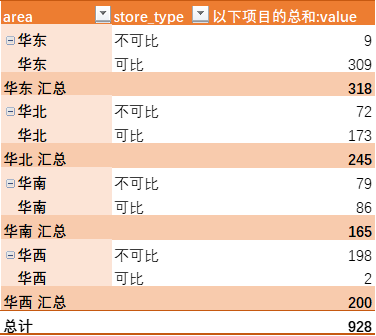
\includegraphics{./picture/data-table/Excel-pivot-groupingsets.png}
\caption{Excel groupingsets透视表}
\end{figure}

\begin{itemize}
\tightlist
\item
  rollup
\end{itemize}

\begin{Shaded}
\begin{Highlighting}[]
\FunctionTok{library}\NormalTok{(magrittr)}
\NormalTok{DT }\OtherTok{\textless{}{-}} \FunctionTok{fread}\NormalTok{(}\StringTok{\textquotesingle{}./data/data{-}table{-}groupingsets.csv\textquotesingle{}}\NormalTok{,}\AttributeTok{encoding =} \StringTok{\textquotesingle{}UTF{-}8\textquotesingle{}}\NormalTok{)}
\NormalTok{(}\FunctionTok{rollup}\NormalTok{(DT,}\AttributeTok{j =}\FunctionTok{list}\NormalTok{(以下项目的总和 }\OtherTok{=}\FunctionTok{sum}\NormalTok{(value)),}\AttributeTok{by =} \FunctionTok{c}\NormalTok{(}\StringTok{"area"}\NormalTok{,}\StringTok{"store\_type"}\NormalTok{),}\AttributeTok{id =} \ConstantTok{TRUE}\NormalTok{) }\SpecialCharTok{\%\textgreater{}\%} \FunctionTok{setorderv}\NormalTok{(}\AttributeTok{cols=}\FunctionTok{c}\NormalTok{(}\StringTok{\textquotesingle{}area\textquotesingle{}}\NormalTok{,}\StringTok{\textquotesingle{}grouping\textquotesingle{}}\NormalTok{),}\AttributeTok{na.last =} \ConstantTok{TRUE}\NormalTok{))}
\end{Highlighting}
\end{Shaded}

通过上述计算,发现计算结果与Excel透视表一样。

\begin{itemize}
\tightlist
\item
  cube
\end{itemize}

观察\texttt{cube()}计算结果与\texttt{rollup()}差异,发现\texttt{cube()}聚合层次更多。

\begin{Shaded}
\begin{Highlighting}[]
\FunctionTok{cube}\NormalTok{(DT,}\AttributeTok{j =} \FunctionTok{sum}\NormalTok{(value),}\AttributeTok{by =} \FunctionTok{c}\NormalTok{(}\StringTok{"area"}\NormalTok{,}\StringTok{"store\_type"}\NormalTok{),}\AttributeTok{id =} \ConstantTok{TRUE}\NormalTok{)}
\end{Highlighting}
\end{Shaded}

\begin{itemize}
\tightlist
\item
  groupingsets
\end{itemize}

根据需要指定指定聚合的层次。

\begin{Shaded}
\begin{Highlighting}[]
\CommentTok{\# 与本例中rollup 结果一致}
\FunctionTok{groupingsets}\NormalTok{(DT,}\AttributeTok{j =} \FunctionTok{sum}\NormalTok{(value),}\AttributeTok{by =} \FunctionTok{c}\NormalTok{(}\StringTok{"area"}\NormalTok{,}\StringTok{"store\_type"}\NormalTok{),}\AttributeTok{sets =} \FunctionTok{list}\NormalTok{(}\StringTok{\textquotesingle{}area\textquotesingle{}}\NormalTok{,}\FunctionTok{c}\NormalTok{(}\StringTok{"area"}\NormalTok{,}\StringTok{"store\_type"}\NormalTok{), }\FunctionTok{character}\NormalTok{()),}\AttributeTok{id =} \ConstantTok{TRUE}\NormalTok{)}

\CommentTok{\# 与本例中cube 结果一致}
\FunctionTok{groupingsets}\NormalTok{(DT,}\AttributeTok{j =} \FunctionTok{sum}\NormalTok{(value),}\AttributeTok{by =} \FunctionTok{c}\NormalTok{(}\StringTok{"area"}\NormalTok{,}\StringTok{"store\_type"}\NormalTok{),}\AttributeTok{sets =} \FunctionTok{list}\NormalTok{(}\StringTok{\textquotesingle{}area\textquotesingle{}}\NormalTok{,}\FunctionTok{c}\NormalTok{(}\StringTok{"area"}\NormalTok{,}\StringTok{"store\_type"}\NormalTok{),}\StringTok{"store\_type"}\NormalTok{, }\FunctionTok{character}\NormalTok{()),}\AttributeTok{id =} \ConstantTok{TRUE}\NormalTok{)}
\end{Highlighting}
\end{Shaded}

\begin{quote}
groupingsets: sets参数,用list()包裹想要聚合的字段组合,最后character(),加上该部分相当于不区分层级全部聚合,用法类似sql中``()''.
\end{quote}

\begin{quote}
SELECT brand, size, sum(sales) FROM items\_sold GROUP BY GROUPING SETS ((brand), (size), ());
\end{quote}

\hypertarget{rleid}{%
\subsection{rleid}\label{rleid}}

该函数根据分组生成长度列。

即将0011001110111101类似这种分组成1 1 2 2 3 3 4 4 4 5 6 6 6 6 7 8。在特定时候是很便捷的一个函数。如在计算股票连续上涨或下跌天数时。

\begin{Shaded}
\begin{Highlighting}[]
\FunctionTok{rleid}\NormalTok{(}\FunctionTok{c}\NormalTok{(}\DecValTok{0}\NormalTok{,}\DecValTok{0}\NormalTok{,}\DecValTok{1}\NormalTok{,}\DecValTok{1}\NormalTok{,}\DecValTok{0}\NormalTok{,}\DecValTok{0}\NormalTok{,}\DecValTok{1}\NormalTok{,}\DecValTok{1}\NormalTok{,}\DecValTok{1}\NormalTok{,}\DecValTok{0}\NormalTok{,}\DecValTok{1}\NormalTok{,}\DecValTok{1}\NormalTok{,}\DecValTok{1}\NormalTok{,}\DecValTok{1}\NormalTok{,}\DecValTok{0}\NormalTok{,}\DecValTok{1}\NormalTok{))}
\end{Highlighting}
\end{Shaded}

用法:

\begin{Shaded}
\begin{Highlighting}[]
\FunctionTok{rleid}\NormalTok{(..., }\AttributeTok{prefix=}\ConstantTok{NULL}\NormalTok{)}
\FunctionTok{rleidv}\NormalTok{(x, }\AttributeTok{cols=}\FunctionTok{seq\_along}\NormalTok{(x), }\AttributeTok{prefix=}\ConstantTok{NULL}\NormalTok{)}
\end{Highlighting}
\end{Shaded}

\begin{Shaded}
\begin{Highlighting}[]
\NormalTok{DT }\OtherTok{=} \FunctionTok{data.table}\NormalTok{(}\AttributeTok{grp=}\FunctionTok{rep}\NormalTok{(}\FunctionTok{c}\NormalTok{(}\StringTok{"A"}\NormalTok{, }\StringTok{"B"}\NormalTok{, }\StringTok{"C"}\NormalTok{, }\StringTok{"A"}\NormalTok{, }\StringTok{"B"}\NormalTok{), }\FunctionTok{c}\NormalTok{(}\DecValTok{2}\NormalTok{,}\DecValTok{2}\NormalTok{,}\DecValTok{3}\NormalTok{,}\DecValTok{1}\NormalTok{,}\DecValTok{2}\NormalTok{)), }\AttributeTok{value=}\DecValTok{1}\SpecialCharTok{:}\DecValTok{10}\NormalTok{)}
\FunctionTok{rleid}\NormalTok{(DT}\SpecialCharTok{$}\NormalTok{grp) }\CommentTok{\# get run{-}length ids}
\FunctionTok{rleidv}\NormalTok{(DT, }\StringTok{"grp"}\NormalTok{) }\CommentTok{\# same as above}
\FunctionTok{rleid}\NormalTok{(DT}\SpecialCharTok{$}\NormalTok{grp, }\AttributeTok{prefix=}\StringTok{"grp"}\NormalTok{) }\CommentTok{\# prefix with \textquotesingle{}grp\textquotesingle{}}
\end{Highlighting}
\end{Shaded}

\hypertarget{shift}{%
\subsection{shift}\label{shift}}

向前或向后功能,通俗来说就是向前或向后移动位置。

示例如下:

\begin{Shaded}
\begin{Highlighting}[]
\NormalTok{x }\OtherTok{=} \DecValTok{1}\SpecialCharTok{:}\DecValTok{5}
\CommentTok{\# lag with n=1 and pad with NA (returns vector)}
\FunctionTok{shift}\NormalTok{(x, }\AttributeTok{n=}\DecValTok{1}\NormalTok{, }\AttributeTok{fill=}\ConstantTok{NA}\NormalTok{, }\AttributeTok{type=}\StringTok{"lag"}\NormalTok{)}
\end{Highlighting}
\end{Shaded}

其中参数n控制偏移量,n正负数和type的参数相对应。, n=-1 and type=`lead' 与 n=1 and type='lag'效果相同。

在data.table上使用:

\begin{Shaded}
\begin{Highlighting}[]
\NormalTok{DT }\OtherTok{=} \FunctionTok{data.table}\NormalTok{(}\AttributeTok{year=}\DecValTok{2010}\SpecialCharTok{:}\DecValTok{2014}\NormalTok{, }\AttributeTok{v1=}\FunctionTok{runif}\NormalTok{(}\DecValTok{5}\NormalTok{), }\AttributeTok{v2=}\DecValTok{1}\SpecialCharTok{:}\DecValTok{5}\NormalTok{, }\AttributeTok{v3=}\NormalTok{letters[}\DecValTok{1}\SpecialCharTok{:}\DecValTok{5}\NormalTok{])}
\NormalTok{cols }\OtherTok{=} \FunctionTok{c}\NormalTok{(}\StringTok{"v1"}\NormalTok{,}\StringTok{"v2"}\NormalTok{,}\StringTok{"v3"}\NormalTok{)}
\NormalTok{anscols }\OtherTok{=} \FunctionTok{paste}\NormalTok{(}\StringTok{"lead"}\NormalTok{, cols, }\AttributeTok{sep=}\StringTok{"\_"}\NormalTok{)}
\NormalTok{DT[, (anscols) }\SpecialCharTok{:}\ErrorTok{=} \FunctionTok{shift}\NormalTok{(.SD, }\DecValTok{1}\NormalTok{, }\DecValTok{0}\NormalTok{, }\StringTok{"lead"}\NormalTok{), .SDcols}\OtherTok{=}\NormalTok{cols]}
\end{Highlighting}
\end{Shaded}

例如求某人连续消费时间间隔天数时:

\begin{Shaded}
\begin{Highlighting}[]
\NormalTok{DT }\OtherTok{=} \FunctionTok{data.table}\NormalTok{(}\AttributeTok{dates =}\NormalTok{lubridate}\SpecialCharTok{::}\FunctionTok{ymd}\NormalTok{(}\FunctionTok{c}\NormalTok{(}\DecValTok{20210105}\NormalTok{,}\DecValTok{20210115}\NormalTok{,}\DecValTok{20210124}\NormalTok{,}\DecValTok{20210218}\NormalTok{,}\DecValTok{20210424}\NormalTok{)))}
\NormalTok{DT[,newdate}\SpecialCharTok{:}\ErrorTok{=}\FunctionTok{shift}\NormalTok{(dates)]}
\NormalTok{DT}
\end{Highlighting}
\end{Shaded}

通过构造新列newdate,然后将两列相减\texttt{dates-newdate}即可得到每次购物间隔天数。

\hypertarget{j}{%
\subsection{J}\label{j}}

J 是\texttt{.()},\texttt{list()}等的别名。\texttt{SJ}是排序连接,\texttt{CJ}是交叉连接。

用法:

\begin{Shaded}
\begin{Highlighting}[]
\CommentTok{\# DT[J(...)]                          \# J() only for use inside DT[...]}
\CommentTok{\# DT[.(...)]                          \# .() only for use inside DT[...]}
\CommentTok{\# DT[list(...)]                       \# same; .(), list() and J() are identical}
\FunctionTok{SJ}\NormalTok{(...)                             }\CommentTok{\# DT[SJ(...)]}
\FunctionTok{CJ}\NormalTok{(..., }\AttributeTok{sorted=}\ConstantTok{TRUE}\NormalTok{, }\AttributeTok{unique=}\ConstantTok{FALSE}\NormalTok{)  }\CommentTok{\# DT[CJ(...)]}
\end{Highlighting}
\end{Shaded}

\begin{itemize}
\tightlist
\item
  CJ
\end{itemize}

我喜欢用\texttt{CJ()}函数创建笛卡尔积表。例如在商品运营中,时常需要将门店和商品形成笛卡尔积表,相比起\texttt{dplyr::full\_join()} ,\texttt{data.table::merge.data.table(allow.cartesian\ =\ TRUE\ )},\texttt{CJ}更加方便快捷。

\begin{Shaded}
\begin{Highlighting}[]
\CommentTok{\# CJ usage examples}
\FunctionTok{CJ}\NormalTok{(}\FunctionTok{c}\NormalTok{(}\DecValTok{5}\NormalTok{, }\ConstantTok{NA}\NormalTok{, }\DecValTok{1}\NormalTok{), }\FunctionTok{c}\NormalTok{(}\DecValTok{1}\NormalTok{, }\DecValTok{3}\NormalTok{, }\DecValTok{2}\NormalTok{))                 }\CommentTok{\# sorted and keyed data.table}
\CommentTok{\# do.call(CJ, list(c(5, NA, 1), c(1, 3, 2)))  \# same as above}
\CommentTok{\# CJ(c(5, NA, 1), c(1, 3, 2), sorted=FALSE)   \# same order as input, unkeyed}
\end{Highlighting}
\end{Shaded}

\begin{itemize}
\tightlist
\item
  SJ
\end{itemize}

SJ : Sorted Join. The same value as J() but additionally setkey() is called on all columns in the order they were passed to SJ. For efficiency, to invoke a binary merge rather than a repeated binary full search for each row of i.

\hypertarget{ux5c0fux6280ux5de7}{%
\section{小技巧}\label{ux5c0fux6280ux5de7}}

\hypertarget{ux7528ux6291ux5236ux4e2dux95f4ux8fc7ux7a0bux8f93ux51fa}{%
\subsection{用\{\}抑制中间过程输出}\label{ux7528ux6291ux5236ux4e2dux95f4ux8fc7ux7a0bux8f93ux51fa}}

默认只返回未命名花括号中定义的最后一个对象。

\begin{Shaded}
\begin{Highlighting}[]
\NormalTok{dt }\OtherTok{\textless{}{-}} \FunctionTok{data.table}\NormalTok{(mtcars)}
\NormalTok{dt[,\{tmp1}\OtherTok{=}\FunctionTok{mean}\NormalTok{(mpg); tmp2}\OtherTok{=}\FunctionTok{mean}\NormalTok{(}\FunctionTok{abs}\NormalTok{(mpg}\SpecialCharTok{{-}}\NormalTok{tmp1)); tmp3}\OtherTok{=}\FunctionTok{round}\NormalTok{(tmp2, }\DecValTok{2}\NormalTok{)\}, by}\OtherTok{=}\NormalTok{cyl]}
\end{Highlighting}
\end{Shaded}

在我不知道上述技巧之前,我可能的操作是

\begin{Shaded}
\begin{Highlighting}[]
\NormalTok{dt }\OtherTok{\textless{}{-}} \FunctionTok{data.table}\NormalTok{(mtcars)}
\NormalTok{res }\OtherTok{\textless{}{-}}\NormalTok{ dt[,tmp1}\SpecialCharTok{:}\ErrorTok{=}\FunctionTok{mean}\NormalTok{(mpg), by}\OtherTok{=}\NormalTok{cyl][,.(}\AttributeTok{tmp2=}\FunctionTok{mean}\NormalTok{(}\FunctionTok{abs}\NormalTok{(mpg}\SpecialCharTok{{-}}\NormalTok{tmp1))), by}\OtherTok{=}\NormalTok{.(cyl)]}
\NormalTok{res[,.(}\FunctionTok{round}\NormalTok{(tmp2,}\DecValTok{2}\NormalTok{)),by}\OtherTok{=}\NormalTok{.(cyl)][]}
\end{Highlighting}
\end{Shaded}

保留中间变量

\begin{Shaded}
\begin{Highlighting}[]
\NormalTok{dt[,\{tmp1}\OtherTok{=}\FunctionTok{mean}\NormalTok{(mpg); tmp2}\OtherTok{=}\FunctionTok{mean}\NormalTok{(}\FunctionTok{abs}\NormalTok{(mpg}\SpecialCharTok{{-}}\NormalTok{tmp1)); tmp3}\OtherTok{=}\FunctionTok{round}\NormalTok{(tmp2, }\DecValTok{2}\NormalTok{); }\FunctionTok{list}\NormalTok{(}\AttributeTok{tmp2=}\NormalTok{tmp2, }\AttributeTok{tmp3=}\NormalTok{tmp3)\}, by}\OtherTok{=}\NormalTok{cyl][]}
\end{Highlighting}
\end{Shaded}

不写分号的方式

\begin{Shaded}
\begin{Highlighting}[]
\NormalTok{dt[,\{tmp1}\OtherTok{=}\FunctionTok{mean}\NormalTok{(mpg)}
\NormalTok{     tmp2}\OtherTok{=}\FunctionTok{mean}\NormalTok{(}\FunctionTok{abs}\NormalTok{(mpg}\SpecialCharTok{{-}}\NormalTok{tmp1))}
\NormalTok{     tmp3}\OtherTok{=}\FunctionTok{round}\NormalTok{(tmp2, }\DecValTok{2}\NormalTok{)}
     \FunctionTok{list}\NormalTok{(}\AttributeTok{tmp2=}\NormalTok{tmp2, }\AttributeTok{tmp3=}\NormalTok{tmp3)\},}
\NormalTok{   by}\OtherTok{=}\NormalTok{cyl][]}
\end{Highlighting}
\end{Shaded}

\hypertarget{ux4f7fux7528ux6253ux5370data.table}{%
\subsection{使用{[}{]}打印data.table}\label{ux4f7fux7528ux6253ux5370data.table}}

在测试代码查看结果时很有用。

\begin{Shaded}
\begin{Highlighting}[]
\NormalTok{df }\OtherTok{\textless{}{-}} \FunctionTok{head}\NormalTok{(mtcars) }\CommentTok{\# doesn\textquotesingle{}t print}
\NormalTok{(df }\OtherTok{\textless{}{-}} \FunctionTok{head}\NormalTok{(mtcars)) }\CommentTok{\# does print}
\end{Highlighting}
\end{Shaded}

\begin{Shaded}
\begin{Highlighting}[]
\CommentTok{\# data.table way of printing after an assignment}
\NormalTok{dt }\OtherTok{\textless{}{-}} \FunctionTok{data.table}\NormalTok{(}\FunctionTok{head}\NormalTok{(mtcars)) }\CommentTok{\# doesn\textquotesingle{}t print}
\NormalTok{dt[,hp2wt}\SpecialCharTok{:}\ErrorTok{=}\NormalTok{hp}\SpecialCharTok{/}\NormalTok{wt][] }\CommentTok{\# does print}
\end{Highlighting}
\end{Shaded}

\hypertarget{ux8fd0ux7528}{%
\section{运用}\label{ux8fd0ux7528}}

\hypertarget{ux81eaux5b9aux4e49ux51fdux6570ux8ba1ux7b97}{%
\subsection{自定义函数计算}\label{ux81eaux5b9aux4e49ux51fdux6570ux8ba1ux7b97}}

1.自定义函数处理列

按照自定义函数计算修改单列或多列

\begin{Shaded}
\begin{Highlighting}[]
\CommentTok{\# 测试函数}

\NormalTok{fun }\OtherTok{\textless{}{-}} \ControlFlowTok{function}\NormalTok{(x)\{}
\NormalTok{  x }\OtherTok{\textless{}{-}}\NormalTok{ x}\SpecialCharTok{\^{}}\DecValTok{2}\SpecialCharTok{+}\DecValTok{1}
\NormalTok{\}}

\NormalTok{DT }\OtherTok{\textless{}{-}}  \FunctionTok{data.table}\NormalTok{(}\AttributeTok{x=}\FunctionTok{rep}\NormalTok{(}\FunctionTok{c}\NormalTok{(}\StringTok{"b"}\NormalTok{,}\StringTok{"a"}\NormalTok{,}\StringTok{"c"}\NormalTok{),}\AttributeTok{each=}\DecValTok{3}\NormalTok{), }\AttributeTok{v=}\FunctionTok{c}\NormalTok{(}\DecValTok{1}\NormalTok{,}\DecValTok{1}\NormalTok{,}\DecValTok{1}\NormalTok{,}\DecValTok{2}\NormalTok{,}\DecValTok{2}\NormalTok{,}\DecValTok{1}\NormalTok{,}\DecValTok{1}\NormalTok{,}\DecValTok{2}\NormalTok{,}\DecValTok{2}\NormalTok{), }\AttributeTok{y=}\FunctionTok{c}\NormalTok{(}\DecValTok{1}\NormalTok{,}\DecValTok{3}\NormalTok{,}\DecValTok{6}\NormalTok{), }\AttributeTok{a=}\DecValTok{1}\SpecialCharTok{:}\DecValTok{9}\NormalTok{, }\AttributeTok{b=}\DecValTok{9}\SpecialCharTok{:}\DecValTok{1}\NormalTok{)}

\NormalTok{DT[,.(}\AttributeTok{newcol=}\FunctionTok{fun}\NormalTok{(y)),by}\OtherTok{=}\NormalTok{.(x)]}

\CommentTok{\#Not run}
\CommentTok{\#DT[,lapply(.SD,fun),.SDcols=c(\textquotesingle{}y\textquotesingle{},\textquotesingle{}a\textquotesingle{}),by=.(x)] \#多列参与计算}


\CommentTok{\# 批量修改列}
\CommentTok{\#Not run}

\CommentTok{\# myfun \textless{}{-} function(x)\{}
\CommentTok{\#   return(x)}
\CommentTok{\# \}}
\CommentTok{\# }
\CommentTok{\# dt \textless{}{-} dt[,colnames(dt):=lapply(.SD[,1:ncol(dt)],myfun)] \#很重要的用法}
\end{Highlighting}
\end{Shaded}

\hypertarget{ux5e26ux6c47ux603bux7684ux805aux5408ux8fd0ux7b97}{%
\subsection{带汇总的聚合运算}\label{ux5e26ux6c47ux603bux7684ux805aux5408ux8fd0ux7b97}}

按照by的字段级别汇总.

\begin{enumerate}
\def\labelenumi{\arabic{enumi}.}
\tightlist
\item
  rollup
\end{enumerate}

分组聚合后设置id=TRUE将各个级别的汇总显示清晰,当by字段只有一个是和正常聚合计算没有区别.以下是官方案例.

\begin{Shaded}
\begin{Highlighting}[]
\CommentTok{\#Usage}
\CommentTok{\#rollup(x, j, by, .SDcols, id = FALSE, ...)}
\NormalTok{n }\OtherTok{=}\NormalTok{ 24L}
\FunctionTok{set.seed}\NormalTok{(}\DecValTok{25}\NormalTok{)}
\NormalTok{DT }\OtherTok{\textless{}{-}} \FunctionTok{data.table}\NormalTok{(}
    \AttributeTok{color =} \FunctionTok{sample}\NormalTok{(}\FunctionTok{c}\NormalTok{(}\StringTok{"green"}\NormalTok{,}\StringTok{"yellow"}\NormalTok{,}\StringTok{"red"}\NormalTok{), n, }\ConstantTok{TRUE}\NormalTok{),}
    \AttributeTok{year =} \FunctionTok{as.Date}\NormalTok{(}\FunctionTok{sample}\NormalTok{(}\FunctionTok{paste0}\NormalTok{(}\DecValTok{2011}\SpecialCharTok{:}\DecValTok{2015}\NormalTok{,}\StringTok{"{-}01{-}01"}\NormalTok{), n, }\ConstantTok{TRUE}\NormalTok{)),}
    \AttributeTok{status =} \FunctionTok{as.factor}\NormalTok{(}\FunctionTok{sample}\NormalTok{(}\FunctionTok{c}\NormalTok{(}\StringTok{"removed"}\NormalTok{,}\StringTok{"active"}\NormalTok{,}\StringTok{"inactive"}\NormalTok{,}\StringTok{"archived"}\NormalTok{), n, }\ConstantTok{TRUE}\NormalTok{)),}
    \AttributeTok{amount =} \FunctionTok{sample}\NormalTok{(}\DecValTok{1}\SpecialCharTok{:}\DecValTok{5}\NormalTok{, n, }\ConstantTok{TRUE}\NormalTok{),}
    \AttributeTok{value =} \FunctionTok{sample}\NormalTok{(}\FunctionTok{c}\NormalTok{(}\DecValTok{3}\NormalTok{, }\FloatTok{3.5}\NormalTok{, }\FloatTok{2.5}\NormalTok{, }\DecValTok{2}\NormalTok{), n, }\ConstantTok{TRUE}\NormalTok{)}
\NormalTok{)}
\FunctionTok{rollup}\NormalTok{(DT, }\AttributeTok{j =} \FunctionTok{sum}\NormalTok{(value), }\AttributeTok{by =} \FunctionTok{c}\NormalTok{(}\StringTok{"color"}\NormalTok{,}\StringTok{"year"}\NormalTok{,}\StringTok{"status"}\NormalTok{)) }\CommentTok{\# default id=FALSE}
\CommentTok{\#rollup(DT, j = sum(value), by = c("color","year","status"), id=TRUE)}
\end{Highlighting}
\end{Shaded}

个人运用,实际工作中常常需要汇总项,汇总项在Excel透视表中很简单,在R中我之前是构造重复的数据源聚合汇总出现汇总项,极大浪费内存,运算速度减慢.

\begin{itemize}
\tightlist
\item
  新方法 rollup
\end{itemize}

\begin{Shaded}
\begin{Highlighting}[]
\FunctionTok{set.seed}\NormalTok{(}\DecValTok{25}\NormalTok{)}
\NormalTok{N }\OtherTok{\textless{}{-}} \DecValTok{1000}
\NormalTok{dt }\OtherTok{\textless{}{-}} \FunctionTok{data.table}\NormalTok{(}\AttributeTok{col1=}\FunctionTok{sample}\NormalTok{(LETTERS[}\DecValTok{1}\SpecialCharTok{:}\DecValTok{5}\NormalTok{],N,}\AttributeTok{replace =}\NormalTok{ T),}\AttributeTok{col2=}\FunctionTok{sample}\NormalTok{(letters[}\DecValTok{1}\SpecialCharTok{:}\DecValTok{5}\NormalTok{],N,}\AttributeTok{replace =}\NormalTok{ T),}\AttributeTok{num=}\DecValTok{1}\SpecialCharTok{:}\NormalTok{N)}

\FunctionTok{rollup}\NormalTok{(dt,}\AttributeTok{j=}\FunctionTok{c}\NormalTok{(}\FunctionTok{list}\NormalTok{(}\FunctionTok{sum}\NormalTok{(num))),}\AttributeTok{by=}\FunctionTok{c}\NormalTok{(}\StringTok{\textquotesingle{}col1\textquotesingle{}}\NormalTok{,}\StringTok{\textquotesingle{}col2\textquotesingle{}}\NormalTok{))}
\CommentTok{\#同上 添加汇总项名称 total}
\CommentTok{\#rollup(dt,j=c(list(total=sum(num))),by=c(\textquotesingle{}col1\textquotesingle{},\textquotesingle{}col2\textquotesingle{}))}
\CommentTok{\#添加id=TRUE参数,多出的grouping 列显示聚合级别}
\CommentTok{\#rollup(dt,j=c(list(total=sum(num))),by=c(\textquotesingle{}col1\textquotesingle{},\textquotesingle{}col2\textquotesingle{}),id=TRUE)}
\end{Highlighting}
\end{Shaded}

2.groupingsets

按照指定字段聚合.包作者说相同与SQL中的 GROUPING SETS 操作.详情参照\href{http://www.postgresql.org/docs/9.5/static/queries-table-expressions.html\#QUERIES-GROUPING-SETS}{postgresql}

\begin{Shaded}
\begin{Highlighting}[]
\NormalTok{res }\OtherTok{\textless{}{-}} \FunctionTok{groupingsets}\NormalTok{(DT, }\AttributeTok{j =} \FunctionTok{c}\NormalTok{(}\FunctionTok{list}\NormalTok{(}\AttributeTok{count=}\NormalTok{.N), }\FunctionTok{lapply}\NormalTok{(.SD, sum)), }\AttributeTok{by =} \FunctionTok{c}\NormalTok{(}\StringTok{"color"}\NormalTok{,}\StringTok{"year"}\NormalTok{,}\StringTok{"status"}\NormalTok{),}
             \AttributeTok{sets =} \FunctionTok{list}\NormalTok{(}\StringTok{"color"}\NormalTok{, }\FunctionTok{c}\NormalTok{(}\StringTok{"year"}\NormalTok{,}\StringTok{"status"}\NormalTok{), }\FunctionTok{character}\NormalTok{()), }\AttributeTok{id=}\ConstantTok{TRUE}\NormalTok{)}
\FunctionTok{head}\NormalTok{(res)}
\end{Highlighting}
\end{Shaded}

注意groupingsets函数中sets参数,用list()包裹想要聚合的字段组合,最后还有一个character(),加上该部分相当于全部聚合.当by只有一个字段时,相当于汇总.用法类似sql中``()''.

上述语句结果等同于下面sql.

\begin{Shaded}
\begin{Highlighting}[]
\KeywordTok{select}\NormalTok{ color ,}\DataTypeTok{year}\NormalTok{, status,}\FunctionTok{count}\NormalTok{(}\OperatorTok{*}\NormalTok{) }\FunctionTok{count}\NormalTok{,}\FunctionTok{sum}\NormalTok{(amount) amount,}\FunctionTok{sum}\NormalTok{(}\FunctionTok{value}\NormalTok{) }\FunctionTok{value} 
\KeywordTok{FROM}\NormalTok{ dbo.DT}
\KeywordTok{GROUP} \KeywordTok{BY}
\FunctionTok{GROUPING}\NormalTok{ SETS(}
\NormalTok{(color),}
\NormalTok{(}\DataTypeTok{year}\NormalTok{,status),}
\NormalTok{() }\CommentTok{{-}{-}{-}{-} 类似 character()}
\NormalTok{)}
\end{Highlighting}
\end{Shaded}

最后还有cube()函数,可?cube查看用法

\hypertarget{ux884cux5217ux8f6cux53d8}{%
\subsection{行列转变}\label{ux884cux5217ux8f6cux53d8}}

\begin{itemize}
\tightlist
\item
  一列变多行
\end{itemize}

用tstrsplit()函数实现

\begin{Shaded}
\begin{Highlighting}[]
\NormalTok{n }\OtherTok{\textless{}{-}} \DecValTok{10}
\NormalTok{dt }\OtherTok{\textless{}{-}} \FunctionTok{data.table}\NormalTok{(}\AttributeTok{name=}\NormalTok{LETTERS[}\DecValTok{1}\SpecialCharTok{:}\NormalTok{n],}\AttributeTok{char=}\FunctionTok{rep}\NormalTok{(}\StringTok{\textquotesingle{}我{-}爱{-}R{-}语{-}言\textquotesingle{}}\NormalTok{),n)}
\NormalTok{res }\OtherTok{\textless{}{-}}\NormalTok{ dt[,.(}\AttributeTok{newcol=}\FunctionTok{tstrsplit}\NormalTok{(char,}\StringTok{\textquotesingle{}{-}\textquotesingle{}}\NormalTok{)),by}\OtherTok{=}\NormalTok{.(name)]}
\FunctionTok{head}\NormalTok{(res)}
\end{Highlighting}
\end{Shaded}

\begin{itemize}
\tightlist
\item
  多行变一列
\end{itemize}

\begin{Shaded}
\begin{Highlighting}[]
\NormalTok{res[,.(}\AttributeTok{char=}\FunctionTok{paste0}\NormalTok{(newcol,}\AttributeTok{collapse =} \StringTok{\textquotesingle{}{-}\textquotesingle{}}\NormalTok{)),by}\OtherTok{=}\NormalTok{.(name)]}
\CommentTok{\#同上}
\CommentTok{\#res[,.(char=stringr::str\_c(newcol,collapse = \textquotesingle{}{-}\textquotesingle{})),by=.(name)]}
\CommentTok{\# A 我{-}爱{-}R{-}语{-}言           }
\CommentTok{\# B 我{-}爱{-}R{-}语{-}言           }
\CommentTok{\# C 我{-}爱{-}R{-}语{-}言           }
\CommentTok{\# D 我{-}爱{-}R{-}语{-}言           }
\CommentTok{\# E 我{-}爱{-}R{-}语{-}言           }
\CommentTok{\# F 我{-}爱{-}R{-}语{-}言           }
\CommentTok{\# G 我{-}爱{-}R{-}语{-}言           }
\CommentTok{\# H 我{-}爱{-}R{-}语{-}言           }
\CommentTok{\# I 我{-}爱{-}R{-}语{-}言           }
\CommentTok{\# J 我{-}爱{-}R{-}语{-}言}
\end{Highlighting}
\end{Shaded}

\hypertarget{database}{%
\chapter{database}\label{database}}

实际工作中,需要从数据库获取数据并清洗,R与数据库有多种交互方式,目前工作中打交道数据库主要是MSSQL,Oracle,mysql等,本文主要从以上数据库介绍记录``R与数据库的连接''。

R中与数据库交互的包主要有DBI,RODBC,RMySQL,ROracle,odbc等包。DBI库在查询或上传工作中效率比RODBC高,特别数据量较大时,上传效率差异巨大,具体\href{https://github.com/r-dbi/odbc}{差异}请点击查看详情。

即使你暂时没有用数据库,也建议你未来用数据库存储数据,尤其是当有一定数据量时;在我最开始接触数据时,数据一般保存在Excel,那时候数据量大概在50万行左右,当公式较多,尤其时需要大批量vlookup时,Excel表格将会很卡顿。

\hypertarget{ux5b89ux88c5ux6570ux636eux5e93}{%
\section{安装数据库}\label{ux5b89ux88c5ux6570ux636eux5e93}}

如果暂时没有数据库使用经验,如果是使用Windows系统,直接去微软官网下载安装数据库即可。如果决定用R做数据分析相关工作,尤其时商业环境下,使用数据库有较强的必要性。安装数据库后,利用数据库做数据分析的练习测试也是不错的体验。另外也可以积累ETL相关经验。

仅简单介绍 MS SQL Server 安装

\begin{itemize}
\tightlist
\item
  Win环境下安装
\end{itemize}

MS\href{https://www.microsoft.com/zh-cn/sql-server/sql-server-downloads}{下载},选择开发版或精简版(Developer、Express)其中一个版本下载即可。

\begin{figure}
\centering

\includegraphics{./picture/chap2/ms install.png}
\caption{数据库下载}
\end{figure}

成功下载后,按照提示一步步确认即可安装成功。另外使用\texttt{SSMS}工具,微软配套的MS SQL SERVER数据库链接工具连接数据库。至于详细的数据库配置尤其是远程连接、账户等信息请自行查阅相关资料。

\begin{itemize}
\tightlist
\item
  Linux环境下安装
\end{itemize}

\href{https://docs.microsoft.com/zh-cn/sql/linux/sql-server-linux-setup?view=sql-server-ver15}{官网安装指南}

以下用于 SQL Server 2019 的命令指向 Ubuntu 20.04 存储库。 如果使用的是 Ubuntu 18.04 或 16.04,请将以下路径更改为 /ubuntu/18.04/ 或 /ubuntu/16.04/,而不是 /ubuntu/20.04/。

\begin{Shaded}
\begin{Highlighting}[]
\CommentTok{\# 导入公共存储库的密钥}
\FunctionTok{wget} \AttributeTok{{-}qO{-}}\NormalTok{ https://packages.microsoft.com/keys/microsoft.asc }\KeywordTok{|} \FunctionTok{sudo}\NormalTok{ apt{-}key add }\AttributeTok{{-}}

\CommentTok{\# 为 SQL Server 2019 注册 Microsoft SQL Server Ubuntu 存储库}
\FunctionTok{sudo}\NormalTok{ add{-}apt{-}repository }\StringTok{"}\VariableTok{$(}\FunctionTok{wget} \AttributeTok{{-}qO{-}}\NormalTok{ https://packages.microsoft.com/config/ubuntu/20.04/mssql{-}server{-}2019.list}\VariableTok{)}\StringTok{"}

\CommentTok{\# sudo add{-}apt{-}repository "$(wget {-}qO{-} https://packages.microsoft.com/config/ubuntu/18.04/mssql{-}server{-}2019.list)"}

\CommentTok{\# 安装 SQL Server}
\FunctionTok{sudo}\NormalTok{ apt{-}get update}
\FunctionTok{sudo}\NormalTok{ apt{-}get install }\AttributeTok{{-}y}\NormalTok{ mssql{-}server}

\CommentTok{\# 验证服务是否运行}
\ExtensionTok{systemctl}\NormalTok{ status mssql{-}server }\AttributeTok{{-}{-}no{-}pager}
\end{Highlighting}
\end{Shaded}

至于其他如安装sql server 命令行工具请\href{https://docs.microsoft.com/zh-cn/sql/linux/quickstart-install-connect-ubuntu?view=sql-server-linux-ver15\&preserve-view=true}{查阅官网安装}。

接下来我们就R语言与数据库的交互包展开介绍。

\hypertarget{dbi}{%
\section{DBI}\label{dbi}}

\hypertarget{ux5b89ux88c5-4}{%
\subsection{安装}\label{ux5b89ux88c5-4}}

\begin{Shaded}
\begin{Highlighting}[]
\FunctionTok{install.packages}\NormalTok{(}\StringTok{\textquotesingle{}DBI\textquotesingle{}}\NormalTok{)}
\end{Highlighting}
\end{Shaded}

\hypertarget{ux8fdeux63a5ux6570ux636eux5e93}{%
\subsection{连接数据库}\label{ux8fdeux63a5ux6570ux636eux5e93}}

\begin{itemize}
\tightlist
\item
  连接MS SQL SERVER
\end{itemize}

通过以下代码即可连接到服务器172.16.88.2(即IP地址)的数据库,成功连接后即可与数据库交互。

\begin{Shaded}
\begin{Highlighting}[]
\FunctionTok{library}\NormalTok{(DBI)}
\NormalTok{con }\OtherTok{\textless{}{-}} \FunctionTok{dbConnect}\NormalTok{(}
  \AttributeTok{drv =}\NormalTok{ odbc}\SpecialCharTok{::}\FunctionTok{odbc}\NormalTok{(), }\AttributeTok{Driver =} \StringTok{"SQL Server"}\NormalTok{, }\AttributeTok{server =} \StringTok{"172.16.88.2"}\NormalTok{,}\AttributeTok{database =} \StringTok{"spb"}\NormalTok{, }\AttributeTok{uid =} \StringTok{"zhongyf"}\NormalTok{, }\AttributeTok{pwd =} \StringTok{"Zyf123456"}
\NormalTok{)}
\end{Highlighting}
\end{Shaded}

如果你用windows系统,通过DBI包连接数据库发现乱码时,根据数据库编码指定encoding参数即可,常规在win下连接sqlserver设置encoding = ``GBK''。

\begin{Shaded}
\begin{Highlighting}[]
\FunctionTok{library}\NormalTok{(DBI)}
\CommentTok{\#根据数据库编码方式指定encoding}
\NormalTok{con }\OtherTok{\textless{}{-}} \FunctionTok{dbConnect}\NormalTok{(}
  \AttributeTok{drv =}\NormalTok{ odbc}\SpecialCharTok{::}\FunctionTok{odbc}\NormalTok{(), }\AttributeTok{Driver =} \StringTok{"SQL Server"}\NormalTok{, }\AttributeTok{server =} \StringTok{"172.16.88.2"}\NormalTok{,}
  \AttributeTok{database =} \StringTok{"spb"}\NormalTok{, }\AttributeTok{uid =} \StringTok{"zhongyf"}\NormalTok{, }\AttributeTok{pwd =} \StringTok{"Zyf123456"}\NormalTok{, }\AttributeTok{encoding =} \StringTok{"GBK"}
\NormalTok{)}
\CommentTok{\# 查看本机可用驱动 如缺少相应驱动则安装,ODBC Driver 17 for SQL Server 就是个人安装的驱动}

\NormalTok{Drivers\_tbl }\OtherTok{\textless{}{-}}\NormalTok{ odbc}\SpecialCharTok{::}\FunctionTok{odbcListDrivers}\NormalTok{() }
\FunctionTok{head}\NormalTok{(Drivers\_tbl)}
\end{Highlighting}
\end{Shaded}

查询数据库编码方式,从而选择连接数据库时相应的编码方式。

\begin{Shaded}
\begin{Highlighting}[]
\NormalTok{con }\OtherTok{\textless{}{-}} \FunctionTok{dbConnect}\NormalTok{(}
  \AttributeTok{drv =}\NormalTok{ odbc}\SpecialCharTok{::}\FunctionTok{odbc}\NormalTok{(), }\AttributeTok{Driver =} \StringTok{"ODBC Driver 17 for SQL Server"}\NormalTok{,}
  \AttributeTok{server =} \StringTok{"172.16.88.2"}\NormalTok{, }\AttributeTok{database =} \StringTok{"spb"}\NormalTok{, }\AttributeTok{uid =} \StringTok{"zhongyf"}\NormalTok{, }\AttributeTok{pwd =} \StringTok{"Zyf123456"}
\NormalTok{)}

\CommentTok{\#查看编码是否是936 代表中文简体}
\NormalTok{sql }\OtherTok{\textless{}{-}} \StringTok{"SELECT COLLATIONPROPERTY( \textquotesingle{}chinese\_prc\_ci\_as\textquotesingle{}, \textquotesingle{}codepage\textquotesingle{} )"}

\FunctionTok{dbGetQuery}\NormalTok{(con,sql)}

\CommentTok{\# same above}
\CommentTok{\# dbExecute(con,sql)}

\CommentTok{\# 用完后记得关闭数据库连接}
\NormalTok{DBI}\SpecialCharTok{::}\FunctionTok{dbDisconnect}\NormalTok{(con)}
\end{Highlighting}
\end{Shaded}

\begin{itemize}
\tightlist
\item
  连接mysql
\end{itemize}

\texttt{MySQL()}函数来源\texttt{RMySQL}包,用来创建\texttt{\textless{}MySQLDriver\textgreater{}}驱动,以下代码可连接到阿里云的MySQL数据库。

\begin{Shaded}
\begin{Highlighting}[]
\FunctionTok{library}\NormalTok{(RMySQL)}
\NormalTok{con }\OtherTok{\textless{}{-}} \FunctionTok{dbConnect}\NormalTok{(}\FunctionTok{MySQL}\NormalTok{(),}
  \AttributeTok{dbname =} \StringTok{"test"}\NormalTok{, }\AttributeTok{user =} \StringTok{"test\_admin"}\NormalTok{, }\AttributeTok{password =} \StringTok{"30HL1234M7\#¥lD6gxjB"}\NormalTok{,}
  \AttributeTok{host =} \StringTok{"prd{-}public{-}mypersonal.mysql.test.zhangjiabei.rds.aliyuncs.com"}
\NormalTok{)}
\end{Highlighting}
\end{Shaded}

或者通过本地已安装驱动连接数据库

\begin{Shaded}
\begin{Highlighting}[]
\NormalTok{con }\OtherTok{\textless{}{-}}\NormalTok{ DBI}\SpecialCharTok{::}\FunctionTok{dbConnect}\NormalTok{(odbc}\SpecialCharTok{::}\FunctionTok{odbc}\NormalTok{(),}
  \AttributeTok{Driver =} \StringTok{"MySQL ODBC 8.0 Unicode Driver"}\NormalTok{,}
  \AttributeTok{Server =} \StringTok{"localhost"}\NormalTok{, }\AttributeTok{UID =} \StringTok{"root"}\NormalTok{, }\AttributeTok{PWD =} \StringTok{"123456"}\NormalTok{, }\AttributeTok{Database =} \StringTok{"mysql"}\NormalTok{,}
  \AttributeTok{Port =} \DecValTok{3306}
\NormalTok{)}
\end{Highlighting}
\end{Shaded}

mysql数据库默认端口是3306,访问不通时记得检查3306端口是否开放。

\hypertarget{ux6267ux884csqlux4efbux52a1}{%
\subsection{执行sql任务}\label{ux6267ux884csqlux4efbux52a1}}

dbGetQuery()函数处理由DBI包创建的con连接查询任务,dbExecute()执行一些数据库任务

\begin{Shaded}
\begin{Highlighting}[]
\CommentTok{\# dbGetQuery 直接查询}
\NormalTok{res\_table }\OtherTok{\textless{}{-}} \FunctionTok{dbGetQuery}\NormalTok{(con,}\StringTok{\textquotesingle{}select * from table\textquotesingle{}}\NormalTok{) }\CommentTok{\#直接获取sql查询结果}

\CommentTok{\#dbReadTable直接读取}
\FunctionTok{dbReadTable}\NormalTok{(con,}\StringTok{\textquotesingle{}tbl\_name\textquotesingle{}}\NormalTok{) }\CommentTok{\#直接读取数据库中某表}

\CommentTok{\# dbSendQuery 执行一个查询任务 }
\NormalTok{res }\OtherTok{\textless{}{-}} \FunctionTok{dbSendQuery}\NormalTok{(}\AttributeTok{conn =}\NormalTok{ con,}\AttributeTok{statement =} \StringTok{\textquotesingle{}select * FROM tab\textquotesingle{}}\NormalTok{)}
\FunctionTok{dbFetch}\NormalTok{(res)}
\FunctionTok{dbClearResult}\NormalTok{(res)}

\CommentTok{\# dbExecute}
\FunctionTok{dbExecute}\NormalTok{(con,}\StringTok{\textquotesingle{}delete from table where num \textless{}=1000\textquotesingle{}}\NormalTok{) }\CommentTok{\#类似任务}

\CommentTok{\# dbWriteTable()}
\CommentTok{\# 上传数据,指定表名,需上传的数据框df,overwrite是否覆盖,append是否可追加}
\FunctionTok{dbWriteTable}\NormalTok{(}\AttributeTok{conn =}\NormalTok{ con,}\AttributeTok{name =} \StringTok{\textquotesingle{}表名\textquotesingle{}}\NormalTok{,}\AttributeTok{value =}\NormalTok{ df,}\AttributeTok{overwrite=}\NormalTok{TURE,}\AttributeTok{append=}\ConstantTok{FALSE}\NormalTok{)}
\end{Highlighting}
\end{Shaded}

\hypertarget{ux51fdux6570ux4ecbux7ecd}{%
\subsection{函数介绍}\label{ux51fdux6570ux4ecbux7ecd}}

查看数据库信息,查看表名,删除表,关闭连接等常用操作.

\begin{Shaded}
\begin{Highlighting}[]
\NormalTok{con }\OtherTok{\textless{}{-}} \FunctionTok{dbConnect}\NormalTok{(}
  \AttributeTok{drv =}\NormalTok{ odbc}\SpecialCharTok{::}\FunctionTok{odbc}\NormalTok{(),}
  \AttributeTok{Driver =} \StringTok{"ODBC Driver 17 for SQL Server"}\NormalTok{, }\AttributeTok{server =} \StringTok{"172.16.88.2"}\NormalTok{, }
  \AttributeTok{database =} \StringTok{"spb"}\NormalTok{, }\AttributeTok{uid =} \StringTok{"zhongyf"}\NormalTok{, }\AttributeTok{pwd =} \StringTok{"Zyf123456"}\NormalTok{, }\AttributeTok{encoding =} \StringTok{"GBK"}
\NormalTok{)}

\CommentTok{\#查看数据版本连接信息}
\FunctionTok{dbGetInfo}\NormalTok{(con)}

\CommentTok{\# 数据库中的全部表名}
\FunctionTok{dbListTables}\NormalTok{(con) }\CommentTok{\#win下中文表名还是会乱码}

\CommentTok{\# 删除表}
\FunctionTok{dbRemoveTable}\NormalTok{(con,}\StringTok{\textquotesingle{}tbl\_name\textquotesingle{}}\NormalTok{)}

\CommentTok{\# 关闭连接}
\FunctionTok{dbDisconnect}\NormalTok{(con)}
\end{Highlighting}
\end{Shaded}

\hypertarget{odbcux5305}{%
\section{odbc包}\label{odbcux5305}}

官方介绍:Connect to ODBC databases (using the DBI interface)

记录到此时,并不时特别清晰\texttt{odbc}与\texttt{DBI}之间的关系。

odbc可以运用于包括(SQL Server, Oracle, MySQL,PostgreSQL,SQLite)等odbc驱动程序于\texttt{DBI}兼容的接口,相比起来\texttt{DBI}包适用范围更广。

1.安装包

\begin{Shaded}
\begin{Highlighting}[]
\CommentTok{\#安装包}
\FunctionTok{install.packages}\NormalTok{(}\StringTok{\textquotesingle{}odbc\textquotesingle{}}\NormalTok{)}
\end{Highlighting}
\end{Shaded}

2.连接数据库

连接数据库需要注意时区、编码,尤其是涉及到时间时时区如果设置有误,可能导致上传数据错误。

当你在Win系统上连接Sql Server时,如果你使用的数据库是中文环境时,最好设置\texttt{encoding}参数。

如果是linux上通过odbc连接SqlServer,一般情况下可以不用设置编码。如果还是乱码,在连接字符中设置字符编码charset=zh\_CN.GBK,设置为gbk会报错。

\begin{Shaded}
\begin{Highlighting}[]
\FunctionTok{library}\NormalTok{(odbc)}
\NormalTok{con }\OtherTok{\textless{}{-}}\NormalTok{ odbc}\SpecialCharTok{::}\FunctionTok{dbConnect}\NormalTok{(}\FunctionTok{odbc}\NormalTok{(),}
  \AttributeTok{Driver =} \StringTok{"SQL Server"}\NormalTok{, }\AttributeTok{Server =} \StringTok{"Vega"}\NormalTok{, }\AttributeTok{Database =} \StringTok{"ghzy"}\NormalTok{,}
  \AttributeTok{Trusted\_Connection =} \StringTok{"True"}
\NormalTok{) }\CommentTok{\# windows身份认证连接}
\CommentTok{\# con \textless{}{-} dbConnect(odbc::odbc(), .connection\_string = "Driver=\{SQL Server\};}
\CommentTok{\#                                 server=Vega;database=ghzy;uid=zhongyf;pwd=Zyf123456;", timeout = 10)}
\NormalTok{con}
\DocumentationTok{\#\# Not run}
\CommentTok{\# Win}
\NormalTok{con\_spb }\OtherTok{\textless{}{-}} \FunctionTok{dbConnect}\NormalTok{(}\FunctionTok{odbc}\NormalTok{(), }\AttributeTok{.connection\_string =} \StringTok{"driver=\{ODBC Driver 17 for SQL Server\};server=172.16.88.2;database=spb;uid=zhongyf;pwd=Zyf123456"}\NormalTok{, }
                     \AttributeTok{timeout =} \DecValTok{10}\NormalTok{, }\AttributeTok{timezone =} \StringTok{"Asia/Shanghai"}\NormalTok{,}\AttributeTok{encoding =} \StringTok{\textquotesingle{}gbk\textquotesingle{}}\NormalTok{)}
\CommentTok{\#Linux}
\NormalTok{con\_dd }\OtherTok{\textless{}{-}} \FunctionTok{dbConnect}\NormalTok{(odbc}\SpecialCharTok{::}\FunctionTok{odbc}\NormalTok{(), }\AttributeTok{.connection\_string =} \StringTok{"driver=\{ODBC Driver 17 for SQL Server\};server=172.16.88.2;}
\StringTok{                 database=aojo\_dd;uid=wj;pwd=12qw\#$ER;charset=zh\_CN.GBK"}\NormalTok{, }\AttributeTok{timeout =} \DecValTok{10}\NormalTok{)}
\end{Highlighting}
\end{Shaded}

3.查询

\begin{Shaded}
\begin{Highlighting}[]
\NormalTok{dt }\OtherTok{\textless{}{-}}\NormalTok{ odbc}\SpecialCharTok{::}\FunctionTok{dbGetQuery}\NormalTok{(con,}\StringTok{\textquotesingle{}select * from DT\textquotesingle{}}\NormalTok{)}
\FunctionTok{head}\NormalTok{(dt)}
\end{Highlighting}
\end{Shaded}

4.写入数据库

\begin{Shaded}
\begin{Highlighting}[]
\NormalTok{odbc}\SpecialCharTok{::}\FunctionTok{dbWriteTable}\NormalTok{(con,}\AttributeTok{name =} \StringTok{\textquotesingle{}表名\textquotesingle{}}\NormalTok{,}\AttributeTok{value =}\NormalTok{ dt,}\AttributeTok{overwrite =}\NormalTok{ T ) }\CommentTok{\# 是否覆盖}
\NormalTok{odbc}\SpecialCharTok{::}\FunctionTok{dbWriteTable}\NormalTok{(con,}\AttributeTok{name =} \StringTok{\textquotesingle{}表名\textquotesingle{}}\NormalTok{,}\AttributeTok{value =}\NormalTok{ dt,}\AttributeTok{append =}\NormalTok{ T ) }\CommentTok{\# 是否追加}
\end{Highlighting}
\end{Shaded}

\hypertarget{rodbcux5305}{%
\section{RODBC包}\label{rodbcux5305}}

RODBC包是R语言对ODBC数据库接口,可以连接所有的ODBC数据库.

1.安装包

\begin{Shaded}
\begin{Highlighting}[]
\FunctionTok{install.packages}\NormalTok{(}\StringTok{\textquotesingle{}RODBC\textquotesingle{}}\NormalTok{)}
\end{Highlighting}
\end{Shaded}

2.SQL SERVER 数据库举例

\begin{Shaded}
\begin{Highlighting}[]
\FunctionTok{library}\NormalTok{(RODBC)}
\NormalTok{con }\OtherTok{\textless{}{-}} \FunctionTok{odbcDriverConnect}\NormalTok{(}\StringTok{"driver=\{SQL Server\};server=192.168.2.62;database=dbname;uid=zhongyf;pwd=Zyf123456"}\NormalTok{)}
\NormalTok{con}
\NormalTok{RODBC}\SpecialCharTok{::}\FunctionTok{sqlQuery}\NormalTok{(con,}\StringTok{\textquotesingle{}select * from test\textquotesingle{}}\NormalTok{)}
\end{Highlighting}
\end{Shaded}

在WINDOWS机器上,需要知道本机是否有相应数据库的驱动程序.

\begin{itemize}
\tightlist
\item
  查看本机上可用驱动
\end{itemize}

\begin{Shaded}
\begin{Highlighting}[]
\NormalTok{odbc}\SpecialCharTok{::}\FunctionTok{odbcListDrivers}\NormalTok{()}
\end{Highlighting}
\end{Shaded}

\begin{itemize}
\tightlist
\item
  怎样安装驱动
\end{itemize}

请参照\href{https://github.com/r-dbi/odbc\#installation}{驱动安装}

ODBC for sql server driver 下载地址\href{https://docs.microsoft.com/zh-cn/sql/connect/odbc/download-odbc-driver-for-sql-server?view=sql-server-ver15}{地址}

3.数据库字符串

请参照\href{https://www.connectionstrings.com/}{数据库连接字符串}

\begin{Shaded}
\begin{Highlighting}[]
\CommentTok{\#ODBC Driver 17 for SQL Server}
\NormalTok{cn }\OtherTok{\textless{}{-}} \FunctionTok{odbcDriverConnect}\NormalTok{(}\StringTok{"Driver=\{ODBC Driver 17 for SQL Server\};Server=localhost;Database=name;UID=username;PWD=123456;"}\NormalTok{) }\CommentTok{\#server 数据库 UID 数据库账户 PWD 数据库账户密码}
\end{Highlighting}
\end{Shaded}

sql server 请参照\href{https://www.connectionstrings.com/microsoft-odbc-driver-17-for-sql-server/}{sql server连接字符串}

\hypertarget{roracleux5305}{%
\section{ROracle包}\label{roracleux5305}}

在第一次安装这个包时遇到了很多困难,首先需要安装oracle客户端,其次配置好环境变量,最后安装包。R与Oracle的连接需要安装\href{https://www.oracle.com/database/technologies/instant-client.html}{Oracle Instant Client},

\begin{enumerate}
\def\labelenumi{\arabic{enumi}.}
\tightlist
\item
  安装客户端
\end{enumerate}

安装oracle客户端,根据电脑的位数选择相应的32位或64位,根据要连接数据库版本,可以去官网自行下载,本机需要下载的\href{https://www.oracle.com/technetwork/database/enterprise-edition/downloads/112010-win64soft-094461.html}{客户端地址}

\begin{enumerate}
\def\labelenumi{\arabic{enumi}.}
\setcounter{enumi}{1}
\tightlist
\item
  配置环境变量
\end{enumerate}

根据自己所使用的系统,配置环境变量

\begin{verbatim}
OCI_INC='D:\app\zhongyf\product\11.2.0\client_1\oci\include'
OCI_LIB64='D:\app\zhongyf\product\11.2.0\client_1\BIN'
\end{verbatim}

linxu上安装\texttt{Roracle}包,可以参考我的

微信公众号:宇飞的世界

\href{https://mp.weixin.qq.com/s/QLwedZ5mTybqSXdHMTGRIw}{公众号文章连接}

\begin{enumerate}
\def\labelenumi{\arabic{enumi}.}
\setcounter{enumi}{2}
\tightlist
\item
  安装包
\end{enumerate}

安装Roracle包需要配置相应版本的Rtools并添加到环境变量,另外配置两个oracle的环境变量。代码中有注释,按照自己安装版本路径修改。

由于ROracle依赖于Oracle Instant Client,安装之前一定要先安装好客户端。

\begin{Shaded}
\begin{Highlighting}[]
\FunctionTok{install.packages}\NormalTok{(}\StringTok{\textquotesingle{}ROracle\textquotesingle{}}\NormalTok{)}
\end{Highlighting}
\end{Shaded}

\begin{enumerate}
\def\labelenumi{\arabic{enumi}.}
\setcounter{enumi}{3}
\tightlist
\item
  连接数据库
\end{enumerate}

\texttt{Roracle}可以通过\texttt{DBI}包链接,除了驱动和连接字符串有差异,其他部分一样。

\begin{Shaded}
\begin{Highlighting}[]
\FunctionTok{library}\NormalTok{(ROracle)}
\NormalTok{drv }\OtherTok{\textless{}{-}}\FunctionTok{dbDriver}\NormalTok{(}\StringTok{"Oracle"}\NormalTok{)}
\NormalTok{connect.string }\OtherTok{\textless{}{-}} \StringTok{\textquotesingle{}(DESCRIPTION =}
\StringTok{                    (ADDRESS = (PROTOCOL = TCP)(HOST = 192.16.88.129)(PORT = 1521))}
\StringTok{                  (CONNECT\_DATA =}
\StringTok{                      (SERVER = DEDICATED)}
\StringTok{                    (SERVICE\_NAME = bidev)}
\StringTok{                  ))\textquotesingle{}} \CommentTok{\#连接字符串}

\NormalTok{con }\OtherTok{\textless{}{-}} \FunctionTok{dbConnect}\NormalTok{(drv,}\AttributeTok{username =} \StringTok{"query"}\NormalTok{, }\AttributeTok{password =} \StringTok{"query"}\NormalTok{,}\AttributeTok{dbname =}\NormalTok{ connect.string)}
\end{Highlighting}
\end{Shaded}

\begin{enumerate}
\def\labelenumi{\arabic{enumi}.}
\setcounter{enumi}{4}
\tightlist
\item
  乱码问题
\end{enumerate}

如果连接oracle数据库,中文乱码设置以下环境变量即可,或者在启动文件配置该环境变量。

linux下可以在文件Renviron中添加,记得引号,路径为{[}/opt/R/4.0.2/lib/R/etc/Renviron{]}

\begin{Shaded}
\begin{Highlighting}[]
\CommentTok{\# 查询数据库编码}
\NormalTok{select }\FunctionTok{userenv}\NormalTok{(}\StringTok{\textquotesingle{}language\textquotesingle{}}\NormalTok{) from dual}
\FunctionTok{Sys.setenv}\NormalTok{(}\AttributeTok{NLS\_LANG=}\StringTok{"SIMPLIFIED CHINESE\_CHINA.AL32UTF8"}\NormalTok{)}
\end{Highlighting}
\end{Shaded}

\hypertarget{rmysqlux5305}{%
\section{RMySQL包}\label{rmysqlux5305}}

RMySQL包的主要作用可以提供驱动与mysql数据库进行连接,在本机未安装mysql的驱动的情况下.该包正在逐渐被淘汰,可以使用RMariaDB包替换。

\hypertarget{ux5b89ux88c5-5}{%
\subsection{安装}\label{ux5b89ux88c5-5}}

Win系统下直接安装即可,其它平台下需提前安装依赖环境。

\begin{Shaded}
\begin{Highlighting}[]
\CommentTok{\#On recent Debian or Ubuntu install libmariadbclient{-}dev}

\FunctionTok{sudo}\NormalTok{ apt{-}get install }\AttributeTok{{-}y}\NormalTok{ libmariadbclient{-}dev}
\CommentTok{\#On Fedora, CentOS or RHEL we need mariadb{-}devel:}

\FunctionTok{sudo}\NormalTok{ yum install mariadb{-}devel}
\CommentTok{\#On OS{-}X use mariadb{-}connector{-}c from Homebrew:}

\ExtensionTok{brew}\NormalTok{ install mariadb{-}connector{-}c}
\end{Highlighting}
\end{Shaded}

\begin{Shaded}
\begin{Highlighting}[]
\FunctionTok{install.packages}\NormalTok{(}\StringTok{\textquotesingle{}RMySQL\textquotesingle{}}\NormalTok{)}
\end{Highlighting}
\end{Shaded}

\hypertarget{ux8fdeux63a5ux4f7fux7528}{%
\subsection{连接使用}\label{ux8fdeux63a5ux4f7fux7528}}

连接数据库,与上述连接方式基本一致。

\begin{Shaded}
\begin{Highlighting}[]
\FunctionTok{library}\NormalTok{(RMySQL)}
\NormalTok{con }\OtherTok{\textless{}{-}}\NormalTok{ RMySQL}\SpecialCharTok{::}\FunctionTok{dbConnect}\NormalTok{(}\AttributeTok{drv =}\NormalTok{ RMySQL}\SpecialCharTok{::}\FunctionTok{MySQL}\NormalTok{(),}\AttributeTok{host=}\StringTok{\textquotesingle{}localhost\textquotesingle{}}\NormalTok{,}\AttributeTok{dbname=}\StringTok{"mysql"}\NormalTok{,}\AttributeTok{username=}\StringTok{"root"}\NormalTok{,}\AttributeTok{password=}\StringTok{\textquotesingle{}123456\textquotesingle{}}\NormalTok{)}
\end{Highlighting}
\end{Shaded}

\texttt{RMariaDB}包与\texttt{RMySQL}包用法基本一致,在连接时注意驱动的选择即可。

\begin{Shaded}
\begin{Highlighting}[]
\FunctionTok{install.packages}\NormalTok{(}\StringTok{\textquotesingle{}RMariaDB\textquotesingle{}}\NormalTok{)}
\FunctionTok{library}\NormalTok{(RMariaDB)}
\NormalTok{con }\OtherTok{\textless{}{-}}\NormalTok{ RMySQL}\SpecialCharTok{::}\FunctionTok{dbConnect}\NormalTok{(}\AttributeTok{drv =}\NormalTok{ RMariaDB}\SpecialCharTok{::}\FunctionTok{MariaDB}\NormalTok{() ,}\AttributeTok{host=}\StringTok{\textquotesingle{}localhost\textquotesingle{}}\NormalTok{,}\AttributeTok{dbname=}\StringTok{"dbtest"}\NormalTok{,}\AttributeTok{username=}\StringTok{"root"}\NormalTok{,}\AttributeTok{password=}\StringTok{\textquotesingle{}123456\textquotesingle{}}\NormalTok{)}
\end{Highlighting}
\end{Shaded}

\hypertarget{ux5e38ux89c1ux95eeux9898}{%
\section{常见问题}\label{ux5e38ux89c1ux95eeux9898}}

在使用R包连接数据库时有些常见的问题,整理如下:

\hypertarget{ux4e71ux7801ux95eeux9898}{%
\subsection{乱码问题}\label{ux4e71ux7801ux95eeux9898}}

R中中文乱码问题一直都很麻烦,并且常常遇见,尤其是使用win系统时。

\begin{itemize}
\tightlist
\item
  MS SQL SERVER 乱码
\end{itemize}

修改encoding参数,在win系统下,可以考虑使用RODBC包连接查询数据库,因为该包将自动转换编码,不会存在乱码问题。但是上传效率奇慢,为了减少包依赖保持代码一致性使用odbc连接数据库时遇到乱码,在连接数据库时设定encoding即可。

\begin{Shaded}
\begin{Highlighting}[]
\CommentTok{\# win}
\NormalTok{con\_spb }\OtherTok{\textless{}{-}} \FunctionTok{dbConnect}\NormalTok{(}\FunctionTok{odbc}\NormalTok{(),}
  \AttributeTok{.connection\_string =}
    \StringTok{"driver=\{ SQLServer\};server=172.16.88.2;database=spb;uid=zhongyf;pwd=Zyf123456"}\NormalTok{, }
  \AttributeTok{timeout =} \DecValTok{10}\NormalTok{, }\AttributeTok{timezone =} \StringTok{"Asia/Shanghai"}\NormalTok{, }\AttributeTok{encoding =} \StringTok{"gbk"}
\NormalTok{)}

\CommentTok{\# linux }
\NormalTok{con\_spb }\OtherTok{\textless{}{-}} \FunctionTok{dbConnect}\NormalTok{(}\FunctionTok{odbc}\NormalTok{(),}
                     \AttributeTok{.connection\_string =}
                       \StringTok{"driver=\{ODBC Driver 17 for SQL Server\};server=172.16.88.2;database=spb;uid=zhongyf;pwd=Zyf123456"}\NormalTok{, }
                     \AttributeTok{timeout =} \DecValTok{10}\NormalTok{, }\AttributeTok{timezone =} \StringTok{"Asia/Shanghai"}\NormalTok{, }\AttributeTok{encoding =} \StringTok{"utf8"}
\NormalTok{)}
\end{Highlighting}
\end{Shaded}

\begin{itemize}
\tightlist
\item
  MySQL乱码
\end{itemize}

1.代码修改

\begin{Shaded}
\begin{Highlighting}[]
\CommentTok{\#执行查询语句前执行}
\FunctionTok{dbSendQuery}\NormalTok{(con,}\StringTok{\textquotesingle{}SET NAMES gbk\textquotesingle{}}\NormalTok{)}
\end{Highlighting}
\end{Shaded}

2.ODBC配置

如果是通过ODBC数据源连接,可通过配置需改,如下所示:

\begin{figure}
\centering
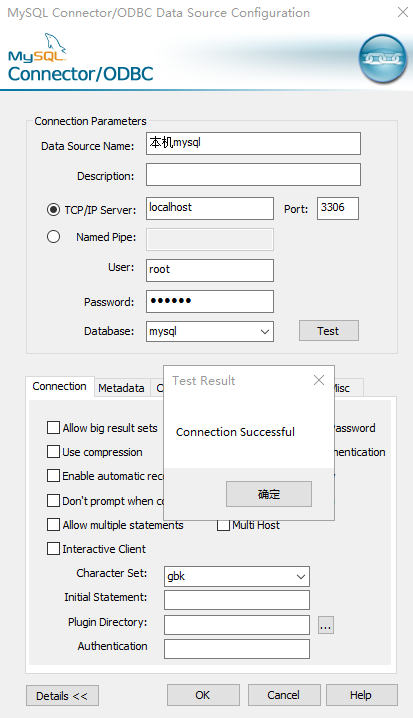
\includegraphics{./picture/chap2/pic1.png}
\caption{ODBC配置截图}
\end{figure}

\hypertarget{ux65e0ux6cd5ux8fdeux63a5ux95eeux9898}{%
\subsection{无法连接问题}\label{ux65e0ux6cd5ux8fdeux63a5ux95eeux9898}}

首先需要装mysql的驱动,确保\texttt{RMySQL}成功安装 如果是测试自己安装的mysql,可以先用Navicat连接,如果出现Authentication plugin `caching\_sha2\_password' cannot be loaded的错误。

可能是由于 mysql8 之前的版本中加密规则是mysql\_native\_password,而在mysql8之后,加密规则是caching\_sha2\_password,通过修改加密规则可解决无法连接问题。

\begin{Shaded}
\begin{Highlighting}[]

\CommentTok{{-}{-}cmd 登录本地数据}
\NormalTok{mysql }\OperatorTok{{-}}\NormalTok{u root }\OperatorTok{{-}}\NormalTok{p}
\CommentTok{{-}{-}输入密码}
\KeywordTok{password}\NormalTok{: }

\CommentTok{{-}{-}执行命令}
\KeywordTok{ALTER} \FunctionTok{USER} \StringTok{\textquotesingle{}root\textquotesingle{}}\NormalTok{@}\StringTok{\textquotesingle{}localhost\textquotesingle{}} \KeywordTok{IDENTIFIED} \KeywordTok{BY} \StringTok{\textquotesingle{}password\textquotesingle{}} \KeywordTok{PASSWORD} \KeywordTok{EXPIRE} \KeywordTok{NEVER}\NormalTok{;   \#修改加密规则 }
\CommentTok{{-}{-}{-}ALTER USER \textquotesingle{}root\textquotesingle{}@\textquotesingle{}\%\textquotesingle{} IDENTIFIED BY \textquotesingle{}password\textquotesingle{} PASSWORD EXPIRE NEVER; 看账号权限注意与上面的区别}

\KeywordTok{ALTER} \FunctionTok{USER} \StringTok{\textquotesingle{}root\textquotesingle{}}\NormalTok{@}\StringTok{\textquotesingle{}localhost\textquotesingle{}} \KeywordTok{IDENTIFIED} \KeywordTok{WITH}\NormalTok{ mysql\_native\_password }\KeywordTok{BY} \StringTok{\textquotesingle{}password\textquotesingle{}}\NormalTok{; \#更新一下用户的密码 }
\end{Highlighting}
\end{Shaded}

\hypertarget{ux8fdcux7a0bux8fdeux63a5}{%
\subsection{远程连接}\label{ux8fdcux7a0bux8fdeux63a5}}

当你需要远程连接时,需要确保数据库的远程连接已经开启。在数据库中开启某账户远程连接权限,在公司的话,数据库连接问题咨询公司的IT人员。自己个人电脑上安装的MS SQL SERVER数据库需要自行开启远程连接。

另外如果是云服务器上搭建的数据库,需要开启数据库端口,如Mysql默认端口3306;如果是阿里云的Rds数据库,找DBA管理员要数据库地址以及端口信息。

\hypertarget{dbplyr}{%
\section{dbplyr}\label{dbplyr}}

\texttt{dbplyr}将\texttt{dplyr}包的函数转化为\texttt{SQL}语句去服务器获取数据;在数据量较大、计算较多时,可以将远程连接数据库中的表当作内存中的数据框使用,当本机内存不够大时,这样做的好处不言而喻。

至于为什么使用\texttt{dbplyr}而不是直接编写\texttt{SQL},因为:

\begin{itemize}
\item
  \texttt{dbplyr}写起来简洁高效,基本跟用\texttt{dplyr}没有差别
\item
  能利用数据库所在服务器的算力,配合上并行计算,在处理大量数据时,大大加快速度。
\item
  不同数据库的语法存在差异,当源数据存在不同数据库时,用R的\texttt{dbplyr}包清洗数据时能加快效率
\item
  通过\texttt{dplyr}动词方便实现复杂的逻辑,当过程越多越复杂时\texttt{dbplyr}的优势越明显,不用一层层嵌套语句。
\end{itemize}

\hypertarget{ux57faux7840ux7528ux6cd5-2}{%
\subsection{基础用法}\label{ux57faux7840ux7528ux6cd5-2}}

\begin{Shaded}
\begin{Highlighting}[]
\FunctionTok{library}\NormalTok{(dplyr)}
\FunctionTok{library}\NormalTok{(dbplyr)}

\NormalTok{mf }\OtherTok{\textless{}{-}} \FunctionTok{memdb\_frame}\NormalTok{(}\AttributeTok{x =} \DecValTok{1}\NormalTok{, }\AttributeTok{y =} \DecValTok{2}\NormalTok{)}

\NormalTok{mf }\SpecialCharTok{\%\textgreater{}\%} 
  \FunctionTok{mutate}\NormalTok{(}
    \AttributeTok{a =}\NormalTok{ y }\SpecialCharTok{*}\NormalTok{ x, }
    \AttributeTok{b =}\NormalTok{ a }\SpecialCharTok{\^{}} \DecValTok{2}\NormalTok{,}
\NormalTok{  ) }\SpecialCharTok{\%\textgreater{}\%} 
  \FunctionTok{show\_query}\NormalTok{()}
\end{Highlighting}
\end{Shaded}

\begin{Shaded}
\begin{Highlighting}[]
\FunctionTok{library}\NormalTok{(dplyr)}
\CommentTok{\#connect database}
\NormalTok{con }\OtherTok{\textless{}{-}}\NormalTok{ DBI}\SpecialCharTok{::}\FunctionTok{dbConnect}\NormalTok{(RSQLite}\SpecialCharTok{::}\FunctionTok{SQLite}\NormalTok{(), }\AttributeTok{path =} \StringTok{":memory:"}\NormalTok{)}
\CommentTok{\# 上传数据}
\FunctionTok{copy\_to}\NormalTok{(con, nycflights13}\SpecialCharTok{::}\NormalTok{flights, }\StringTok{"flights"}\NormalTok{,}
  \AttributeTok{temporary =} \ConstantTok{FALSE}\NormalTok{, }
  \AttributeTok{indexes =} \FunctionTok{list}\NormalTok{(}
    \FunctionTok{c}\NormalTok{(}\StringTok{"year"}\NormalTok{, }\StringTok{"month"}\NormalTok{, }\StringTok{"day"}\NormalTok{), }
    \StringTok{"carrier"}\NormalTok{, }
    \StringTok{"tailnum"}\NormalTok{,}
    \StringTok{"dest"}
\NormalTok{  )}
\NormalTok{)}

\CommentTok{\# 查看库中全部表名}
\CommentTok{\#dbListTables(con)}

\CommentTok{\#tbl()引用表flights}

\NormalTok{flights\_db }\OtherTok{\textless{}{-}} \FunctionTok{tbl}\NormalTok{(con, }\StringTok{"flights"}\NormalTok{)}
\NormalTok{flights\_db}

\CommentTok{\# 开始查询}
\NormalTok{flights\_db }\SpecialCharTok{\%\textgreater{}\%} \FunctionTok{select}\NormalTok{(year}\SpecialCharTok{:}\NormalTok{day, dep\_delay, arr\_delay)}
\NormalTok{flights\_db }\SpecialCharTok{\%\textgreater{}\%} \FunctionTok{filter}\NormalTok{(dep\_delay }\SpecialCharTok{\textgreater{}} \DecValTok{240}\NormalTok{)}
\NormalTok{flights\_db }\SpecialCharTok{\%\textgreater{}\%} 
  \FunctionTok{group\_by}\NormalTok{(dest) }\SpecialCharTok{\%\textgreater{}\%}
  \FunctionTok{summarise}\NormalTok{(}\AttributeTok{delay =} \FunctionTok{mean}\NormalTok{(dep\_time))}
\end{Highlighting}
\end{Shaded}

部分简单不复杂的sql语句可以用dplyr的语法代替.

\begin{Shaded}
\begin{Highlighting}[]
\NormalTok{tailnum\_delay\_db }\OtherTok{\textless{}{-}}\NormalTok{ flights\_db }\SpecialCharTok{\%\textgreater{}\%} 
  \FunctionTok{group\_by}\NormalTok{(tailnum) }\SpecialCharTok{\%\textgreater{}\%}
  \FunctionTok{summarise}\NormalTok{(}
    \AttributeTok{delay =} \FunctionTok{mean}\NormalTok{(arr\_delay,}\AttributeTok{na.rm =}\NormalTok{ T),}
    \AttributeTok{n =} \FunctionTok{n}\NormalTok{()}
\NormalTok{  ) }\SpecialCharTok{\%\textgreater{}\%} 
  \FunctionTok{arrange}\NormalTok{(}\FunctionTok{desc}\NormalTok{(delay)) }\SpecialCharTok{\%\textgreater{}\%}
  \FunctionTok{filter}\NormalTok{(n }\SpecialCharTok{\textgreater{}} \DecValTok{100}\NormalTok{)}
\NormalTok{tailnum\_delay\_db}
\NormalTok{tailnum\_delay\_db }\SpecialCharTok{\%\textgreater{}\%} \FunctionTok{show\_query}\NormalTok{()}
\NormalTok{tailnum\_delay }\OtherTok{\textless{}{-}}\NormalTok{ tailnum\_delay\_db }\SpecialCharTok{\%\textgreater{}\%} \FunctionTok{collect}\NormalTok{() }\CommentTok{\#把数据从数据库加载到R内存中}
\end{Highlighting}
\end{Shaded}

\hypertarget{ux65e0ux6cd5ux6b63ux786eux8f6cux5316}{%
\subsection{无法正确转化}\label{ux65e0ux6cd5ux6b63ux786eux8f6cux5316}}

在使用过程中发现无法识别\texttt{lubridate}包的函数,但是\texttt{dbplyr}对于不认识的函数都将保留。

利用这个特性,可以使用数据库中原生的相关函数:如下所示,在Oracle中\texttt{to\_date}函数

以下的自定义函数可以实现按照想要\texttt{group\_by}的字段汇总金额、数量、吊牌额、折扣率等,其中关于时间周期的筛选就利用了该特性。

\begin{itemize}
\tightlist
\item
  date
\end{itemize}

\begin{Shaded}
\begin{Highlighting}[]
\CommentTok{\#个人写的争对目前公司数仓写的包中获取销售数据的一段代码}
\NormalTok{get\_sales\_data }\OtherTok{\textless{}{-}} \ControlFlowTok{function}\NormalTok{(con,...,start\_date,end\_date,brand\_name,}\AttributeTok{channel\_type =} \ConstantTok{NULL}\NormalTok{ ,}\AttributeTok{area\_name =} \ConstantTok{NULL}\NormalTok{,}\AttributeTok{boss\_name =} \ConstantTok{NULL}\NormalTok{,}\AttributeTok{category\_name =} \ConstantTok{NULL}\NormalTok{,}\AttributeTok{shop\_no =} \ConstantTok{NULL}\NormalTok{)\{}

\NormalTok{  store\_table }\OtherTok{\textless{}{-}} \FunctionTok{store}\NormalTok{(con,}\AttributeTok{brand\_name =}\NormalTok{ brand\_name,}\AttributeTok{channel\_type =}\NormalTok{ channel\_type ,}\AttributeTok{area\_name =}\NormalTok{ area\_name,}\AttributeTok{boss\_name =}\NormalTok{ boss\_name,}\AttributeTok{shop\_no =}\NormalTok{ shop\_no) }\CommentTok{\#门店信息}
  
\NormalTok{  sku\_table }\OtherTok{\textless{}{-}} \FunctionTok{sku}\NormalTok{(con,}\AttributeTok{category\_name =}\NormalTok{  category\_name ) }\CommentTok{\#商品信息}
  
  \FunctionTok{tbl}\NormalTok{(con, }\FunctionTok{in\_schema}\NormalTok{(}\StringTok{"DW"}\NormalTok{, }\StringTok{"DW\_SALE\_SHOP\_F"}\NormalTok{)) }\SpecialCharTok{\%\textgreater{}\%} \CommentTok{\#DW层}
    \FunctionTok{select}\NormalTok{(BILL\_DATE1, SKU\_NO, SHOP\_NO, BILL\_QTY, BILL\_MONEY2, PRICE) }\SpecialCharTok{\%\textgreater{}\%}
    \FunctionTok{filter}\NormalTok{(}\FunctionTok{between}\NormalTok{(}
\NormalTok{      BILL\_DATE1, }\FunctionTok{to\_date}\NormalTok{(start\_date, }\StringTok{"yyyy{-}mm{-}dd"}\NormalTok{),}
      \FunctionTok{to\_date}\NormalTok{(end\_date, }\StringTok{"yyyy{-}mm{-}dd"}\NormalTok{)}
\NormalTok{    )) }\SpecialCharTok{\%\textgreater{}\%}
    \FunctionTok{mutate}\NormalTok{(年 }\OtherTok{=} \FunctionTok{year}\NormalTok{(BILL\_DATE1), 月 }\OtherTok{=} \FunctionTok{month}\NormalTok{(BILL\_DATE1)) }\SpecialCharTok{\%\textgreater{}\%}
    \FunctionTok{inner\_join}\NormalTok{(store\_table) }\SpecialCharTok{\%\textgreater{}\%}
    \FunctionTok{inner\_join}\NormalTok{(sku\_table) }\SpecialCharTok{\%\textgreater{}\%}
    \FunctionTok{group\_by}\NormalTok{(...) }\SpecialCharTok{\%\textgreater{}\%}
    \FunctionTok{summarise}\NormalTok{(}
\NormalTok{      金额 }\OtherTok{=} \FunctionTok{sum}\NormalTok{(BILL\_MONEY2, }\AttributeTok{na.rm =} \ConstantTok{TRUE}\NormalTok{),}
\NormalTok{      数量 }\OtherTok{=} \FunctionTok{sum}\NormalTok{(BILL\_QTY, }\AttributeTok{na.rm =} \ConstantTok{TRUE}\NormalTok{),}
\NormalTok{      吊牌金额 }\OtherTok{=} \FunctionTok{sum}\NormalTok{(BILL\_QTY }\SpecialCharTok{*}\NormalTok{ PRICE, }\AttributeTok{na.rm =} \ConstantTok{TRUE}\NormalTok{)) }\SpecialCharTok{\%\textgreater{}\%}
    \FunctionTok{collect}\NormalTok{() }\SpecialCharTok{\%\textgreater{}\%}
    \FunctionTok{mutate}\NormalTok{(折扣率}\SpecialCharTok{:}\ErrorTok{=}\NormalTok{ 金额 }\SpecialCharTok{/}\NormalTok{ 吊牌金额) }\SpecialCharTok{\%\textgreater{}\%} 
    \FunctionTok{arrange}\NormalTok{(...)}


  \CommentTok{\# return(res)}
\NormalTok{\}}
\end{Highlighting}
\end{Shaded}

\begin{itemize}
\tightlist
\item
  like
\end{itemize}

\begin{Shaded}
\begin{Highlighting}[]
\NormalTok{mf }\SpecialCharTok{\%\textgreater{}\%} 
  \FunctionTok{filter}\NormalTok{(x }\SpecialCharTok{\%LIKE\%} \StringTok{"\%foo\%"}\NormalTok{) }\SpecialCharTok{\%\textgreater{}\%} 
  \FunctionTok{show\_query}\NormalTok{()}
\end{Highlighting}
\end{Shaded}

\begin{itemize}
\tightlist
\item
  特殊用法
\end{itemize}

特殊情况可以使用\texttt{sql()}函数

\begin{Shaded}
\begin{Highlighting}[]
\NormalTok{mf }\SpecialCharTok{\%\textgreater{}\%} 
  \FunctionTok{transmute}\NormalTok{(}\AttributeTok{factorial =} \FunctionTok{sql}\NormalTok{(}\StringTok{"x!"}\NormalTok{)) }\SpecialCharTok{\%\textgreater{}\%} 
  \FunctionTok{show\_query}\NormalTok{()}
\end{Highlighting}
\end{Shaded}

\hypertarget{ux53c2ux8003ux8d44ux6599}{%
\section{参考资料}\label{ux53c2ux8003ux8d44ux6599}}

\texttt{DBI}包资料\url{https://dbi.r-dbi.org/reference/}

\texttt{dbplyr}包资料\url{https://dbplyr.tidyverse.org/}

rstudio关于数据库介绍 \url{https://db.rstudio.com/databases}

数据库连接字符串介绍 \url{https://www.connectionstrings.com/}

个人博客关于Roracle的安装介绍 \url{http://www.zhongyufei.com/2020/07/25/roracle-install/}

\url{https://www.r-consortium.org/blog/2017/05/15/improving-dbi-a-retrospect}

\hypertarget{loop-structure}{%
\chapter{Loop structure}\label{loop-structure}}

实际场景中,当需要重复做某动作时,可运用循环结构。

\hypertarget{ux7b80ux5355ux793aux4f8b}{%
\section{简单示例}\label{ux7b80ux5355ux793aux4f8b}}

利用循环实现1到100连续相加求和

\begin{Shaded}
\begin{Highlighting}[]
\NormalTok{total }\OtherTok{\textless{}{-}} \DecValTok{0}
\ControlFlowTok{for}\NormalTok{(i }\ControlFlowTok{in} \DecValTok{1}\SpecialCharTok{:}\DecValTok{100}\NormalTok{)\{}
\NormalTok{  total }\OtherTok{\textless{}{-}}\NormalTok{ total}\SpecialCharTok{+}\NormalTok{i}
\NormalTok{\}}
\FunctionTok{print}\NormalTok{(}\FunctionTok{paste0}\NormalTok{(}\StringTok{\textquotesingle{}1到100连续相加求和等于:\textquotesingle{}}\NormalTok{,total))}

\CommentTok{\# loop structure}
\CommentTok{\# for (var in seq) \{expr\}}
\end{Highlighting}
\end{Shaded}

\hypertarget{ux5faaux73afux57faux7840}{%
\section{循环基础}\label{ux5faaux73afux57faux7840}}

\hypertarget{ux5faaux73afux7ed3ux6784}{%
\subsection{循环结构}\label{ux5faaux73afux7ed3ux6784}}

R中有三种循环结构:

\begin{itemize}
\tightlist
\item
  Repeat
\end{itemize}

\begin{Shaded}
\begin{Highlighting}[]
\NormalTok{i }\OtherTok{\textless{}{-}} \DecValTok{1}
\NormalTok{total }\OtherTok{\textless{}{-}} \DecValTok{0}
\ControlFlowTok{repeat}\NormalTok{\{}
\NormalTok{  total }\OtherTok{\textless{}{-}}\NormalTok{ total}\SpecialCharTok{+}\NormalTok{i}
\NormalTok{  i }\OtherTok{\textless{}{-}}\NormalTok{ i}\SpecialCharTok{+}\DecValTok{1}
  \ControlFlowTok{if}\NormalTok{(i }\SpecialCharTok{\textgreater{}} \DecValTok{100}\NormalTok{)\{}
    \FunctionTok{print}\NormalTok{(}\FunctionTok{paste0}\NormalTok{(}\StringTok{\textquotesingle{}连续相加求和等于:\textquotesingle{}}\NormalTok{,total))}
    \ControlFlowTok{break}
\NormalTok{  \}}
\NormalTok{\}}
\end{Highlighting}
\end{Shaded}

\begin{itemize}
\tightlist
\item
  while
\end{itemize}

\begin{Shaded}
\begin{Highlighting}[]
\NormalTok{i }\OtherTok{\textless{}{-}} \DecValTok{1}
\NormalTok{total }\OtherTok{\textless{}{-}} \DecValTok{0}
\ControlFlowTok{while}\NormalTok{(i }\SpecialCharTok{\textless{}=} \DecValTok{1000}\NormalTok{)\{}
\NormalTok{  total }\OtherTok{\textless{}{-}}\NormalTok{ total}\SpecialCharTok{+}\NormalTok{i}
\NormalTok{  i }\OtherTok{\textless{}{-}}\NormalTok{ i}\SpecialCharTok{+}\DecValTok{1}
\NormalTok{\}}
\FunctionTok{print}\NormalTok{(}\FunctionTok{paste0}\NormalTok{(}\StringTok{\textquotesingle{}1到1000连续相加求和等于:\textquotesingle{}}\NormalTok{,total))}
\CommentTok{\# not run}
\CommentTok{\# sum(1:1000)}
\end{Highlighting}
\end{Shaded}

\begin{itemize}
\tightlist
\item
  for
\end{itemize}

代码如示例所示

\begin{Shaded}
\begin{Highlighting}[]
\FunctionTok{library}\NormalTok{(tidyverse)}
\NormalTok{df }\OtherTok{\textless{}{-}} \FunctionTok{tibble}\NormalTok{(}
  \AttributeTok{a =} \FunctionTok{rnorm}\NormalTok{(}\DecValTok{10}\NormalTok{),}
  \AttributeTok{b =} \FunctionTok{rnorm}\NormalTok{(}\DecValTok{10}\NormalTok{),}
  \AttributeTok{c =} \FunctionTok{rnorm}\NormalTok{(}\DecValTok{10}\NormalTok{),}
  \AttributeTok{d =} \FunctionTok{rnorm}\NormalTok{(}\DecValTok{10}\NormalTok{)}
\NormalTok{)}

\NormalTok{output }\OtherTok{\textless{}{-}} \FunctionTok{vector}\NormalTok{(}\StringTok{"double"}\NormalTok{, }\FunctionTok{ncol}\NormalTok{(df))  }\CommentTok{\# 1. output}
\ControlFlowTok{for}\NormalTok{ (i }\ControlFlowTok{in} \FunctionTok{seq\_along}\NormalTok{(df)) \{            }\CommentTok{\# 2. sequence}
\NormalTok{  output[[i]] }\OtherTok{\textless{}{-}} \FunctionTok{median}\NormalTok{(df[[i]])      }\CommentTok{\# 3. body}
\NormalTok{\}}
\NormalTok{output}
\end{Highlighting}
\end{Shaded}

循环中尽可能利用R中的向量化,比如指定output的长度,当数据量大的时候效率提升将比较明显,养成向量化的意识对提高代码效率有显著效果.

上面代码中 \texttt{vector}函数创建一个空向量带指定长度,有两个参数,第一个时向量类型(`逻辑',`整数',`双精度','字符'等),第二个是向量长度 \texttt{vector(length=5)},类型默认是逻辑型.

\texttt{seq\_along}可以\texttt{?seq}查看用法.

hadely 解释如下:

You might not have seen seq\_along() before. It's a safe version of the familiar 1:length(l), with an important difference: if you have a zero-length vector, seq\_along() does the right thing:

\begin{Shaded}
\begin{Highlighting}[]
\CommentTok{\#wrong}
\FunctionTok{seq\_along}\NormalTok{(}\FunctionTok{c}\NormalTok{())}
\DecValTok{1}\SpecialCharTok{:}\FunctionTok{length}\NormalTok{(}\FunctionTok{c}\NormalTok{())}

\CommentTok{\# generates the integer sequence 1, 2, ..., length(along.with). (along.with is usually abbreviated to along, and  seq\_along is much faster.)}
\end{Highlighting}
\end{Shaded}

\hypertarget{next-break-ux7528ux6cd5}{%
\subsection{next break 用法}\label{next-break-ux7528ux6cd5}}

\begin{itemize}
\tightlist
\item
  next 用法
\end{itemize}

\begin{Shaded}
\begin{Highlighting}[]
\ControlFlowTok{for}\NormalTok{(i }\ControlFlowTok{in}\NormalTok{ letters[}\DecValTok{1}\SpecialCharTok{:}\DecValTok{6}\NormalTok{] )\{}
  \ControlFlowTok{if}\NormalTok{(i }\SpecialCharTok{==} \StringTok{"d"}\NormalTok{)\{}
  \ControlFlowTok{next}
\NormalTok{  \}}
  \FunctionTok{print}\NormalTok{(i)}
\NormalTok{\}}
\end{Highlighting}
\end{Shaded}

\begin{itemize}
\tightlist
\item
  break 用法
\end{itemize}

可以当条件满足时跳出循环常常与repeat循环结构配合使用。

\hypertarget{ux5d4cux5957ux5faaux73af}{%
\subsection{嵌套循环}\label{ux5d4cux5957ux5faaux73af}}

\begin{Shaded}
\begin{Highlighting}[]
\CommentTok{\# not run}
\NormalTok{v }\OtherTok{\textless{}{-}} \FunctionTok{vector}\NormalTok{(}\AttributeTok{length =} \DecValTok{100}\NormalTok{)}
\ControlFlowTok{for}\NormalTok{(i }\ControlFlowTok{in} \DecValTok{1}\SpecialCharTok{:}\DecValTok{10}\NormalTok{)\{}
  \ControlFlowTok{for}\NormalTok{(j }\ControlFlowTok{in} \DecValTok{1}\SpecialCharTok{:}\DecValTok{10}\NormalTok{)\{}
\NormalTok{    v[i}\SpecialCharTok{*}\NormalTok{j] }\OtherTok{=}\NormalTok{ i }\SpecialCharTok{*}\NormalTok{ j }
\NormalTok{  \}}
\NormalTok{\}}
\end{Highlighting}
\end{Shaded}

\hypertarget{ux5faaux73afux53d8ux5316}{%
\section{循环变化}\label{ux5faaux73afux53d8ux5316}}

\hypertarget{ux4feeux6539ux5df2ux6709ux5bf9ux8c61}{%
\subsection{修改已有对象}\label{ux4feeux6539ux5df2ux6709ux5bf9ux8c61}}

\begin{Shaded}
\begin{Highlighting}[]
\NormalTok{res }\OtherTok{\textless{}{-}} \DecValTok{1}\SpecialCharTok{:}\DecValTok{100}
\ControlFlowTok{for}\NormalTok{(i }\ControlFlowTok{in} \FunctionTok{seq\_along}\NormalTok{(res))\{}
\NormalTok{  res[i] }\OtherTok{\textless{}{-}}\NormalTok{ res[i] }\SpecialCharTok{*}\NormalTok{ i}
\NormalTok{\}}
\FunctionTok{str}\NormalTok{(res)}
\end{Highlighting}
\end{Shaded}

\hypertarget{ux5faaux73afux6a21ux5f0f}{%
\subsection{循环模式}\label{ux5faaux73afux6a21ux5f0f}}

共有三种遍历向量的方法,之前展示的都是遍历数字索引\texttt{for\ (i\ in\ seq\_along(xs))},并使用提取值\texttt{x{[}{[}i{]}{]}}.还有两种方式:

\begin{itemize}
\tightlist
\item
  循环遍历元素
\end{itemize}

\texttt{for(i\ in\ xs)},例如我们需要保存文件时,可以利用这种循环模式

\begin{itemize}
\tightlist
\item
  遍历名称
\end{itemize}

\texttt{for\ (nm\ in\ names(xs))},我们可以使用\texttt{x{[}{[}nm{]}{]}} 该名称访问.当我们要在文件名中使用名称时会比较方便.

\begin{Shaded}
\begin{Highlighting}[]
\NormalTok{results }\OtherTok{\textless{}{-}} \FunctionTok{vector}\NormalTok{(}\StringTok{"list"}\NormalTok{, }\FunctionTok{length}\NormalTok{(x))}
\FunctionTok{names}\NormalTok{(results) }\OtherTok{\textless{}{-}} \FunctionTok{names}\NormalTok{(x)}
\end{Highlighting}
\end{Shaded}

数字索引的循环模式最常用,因为可以根据位置提取名称和值.

\begin{Shaded}
\begin{Highlighting}[]
\ControlFlowTok{for}\NormalTok{ (i }\ControlFlowTok{in} \FunctionTok{seq\_along}\NormalTok{(x)) \{}
\NormalTok{  name }\OtherTok{\textless{}{-}} \FunctionTok{names}\NormalTok{(x)[[i]]}
\NormalTok{  value }\OtherTok{\textless{}{-}}\NormalTok{ x[[i]]}
\NormalTok{\}}
\end{Highlighting}
\end{Shaded}

\hypertarget{ux672aux77e5ux957fux5ea6ux8f93ux51fa}{%
\subsection{未知长度输出}\label{ux672aux77e5ux957fux5ea6ux8f93ux51fa}}

有时候我们的循环我们不确定输出的长度是多少.这样会逐步增加向量的长度,如下所示:

\begin{Shaded}
\begin{Highlighting}[]
\NormalTok{means }\OtherTok{\textless{}{-}} \FunctionTok{c}\NormalTok{(}\DecValTok{0}\NormalTok{, }\DecValTok{1}\NormalTok{, }\DecValTok{2}\NormalTok{)}

\NormalTok{output }\OtherTok{\textless{}{-}} \FunctionTok{double}\NormalTok{()}
\ControlFlowTok{for}\NormalTok{ (i }\ControlFlowTok{in} \FunctionTok{seq\_along}\NormalTok{(means)) \{}
\NormalTok{  n }\OtherTok{\textless{}{-}} \FunctionTok{sample}\NormalTok{(}\DecValTok{100}\NormalTok{, }\DecValTok{1}\NormalTok{)}
\NormalTok{  output }\OtherTok{\textless{}{-}} \FunctionTok{c}\NormalTok{(output, }\FunctionTok{rnorm}\NormalTok{(n, means[[i]]))}
\NormalTok{\}}
\FunctionTok{str}\NormalTok{(output)}
\end{Highlighting}
\end{Shaded}

但是这种方式浪费时间,当数据量大时候效率会很低下.因为时间复杂度为(\(O(n^2)\)).解决方案是将结果保存在列表中,然后在完成循环后合并为单个向量:

\begin{Shaded}
\begin{Highlighting}[]
\NormalTok{out }\OtherTok{\textless{}{-}} \FunctionTok{vector}\NormalTok{(}\StringTok{"list"}\NormalTok{, }\FunctionTok{length}\NormalTok{(means))}
\ControlFlowTok{for}\NormalTok{ (i }\ControlFlowTok{in} \FunctionTok{seq\_along}\NormalTok{(means)) \{}
\NormalTok{  n }\OtherTok{\textless{}{-}} \FunctionTok{sample}\NormalTok{(}\DecValTok{100}\NormalTok{, }\DecValTok{1}\NormalTok{)}
\NormalTok{  out[[i]] }\OtherTok{\textless{}{-}} \FunctionTok{rnorm}\NormalTok{(n, means[[i]])}
\NormalTok{\}}
\FunctionTok{str}\NormalTok{(out)}
\FunctionTok{str}\NormalTok{(}\FunctionTok{unlist}\NormalTok{(out)) }\CommentTok{\#unlist将列表向量化}
\end{Highlighting}
\end{Shaded}

\hypertarget{iteration}{%
\chapter{Iteration}\label{iteration}}

常常需要重复操作同样的功能函数,这时可以用迭代来实现。purrr包提供了一套完整的函数来处理循环迭代,可以有效减少重复性工作和代码。

\url{https://purrr.tidyverse.org/}

\hypertarget{ux7b80ux5355ux7528ux6cd5}{%
\section{简单用法}\label{ux7b80ux5355ux7528ux6cd5}}

\begin{itemize}
\tightlist
\item
  map
\end{itemize}

用map循环迭代,map函数始终返回list对象。

\begin{Shaded}
\begin{Highlighting}[]
\FunctionTok{library}\NormalTok{(tidyverse)}

\CommentTok{\# define function}
\NormalTok{addTen }\OtherTok{\textless{}{-}} \ControlFlowTok{function}\NormalTok{(.x) \{}
  \FunctionTok{return}\NormalTok{(.x }\SpecialCharTok{+} \DecValTok{10}\NormalTok{)}
\NormalTok{\}}

\FunctionTok{map}\NormalTok{(}\AttributeTok{.x =} \FunctionTok{c}\NormalTok{(}\DecValTok{1}\NormalTok{, }\DecValTok{4}\NormalTok{, }\DecValTok{7}\NormalTok{), }\AttributeTok{.f =}\NormalTok{ addTen)}
\CommentTok{\# not run}
\CommentTok{\# map(c(1, 4, 7), addTen) \# same above}
\end{Highlighting}
\end{Shaded}

\begin{itemize}
\tightlist
\item
  map\_dbl
\end{itemize}

用map\_dbl循环迭代,map\_dbl函数返回vector。

\begin{Shaded}
\begin{Highlighting}[]
\CommentTok{\#library(purrr)}
\NormalTok{add1 }\OtherTok{\textless{}{-}} \ControlFlowTok{function}\NormalTok{(x) \{}
\NormalTok{  (x}\SpecialCharTok{+}\DecValTok{1}\NormalTok{)}\SpecialCharTok{*}\NormalTok{x}
\NormalTok{\}}
\NormalTok{result1 }\OtherTok{\textless{}{-}} \FunctionTok{map\_dbl}\NormalTok{(}\DecValTok{1}\SpecialCharTok{:}\DecValTok{1000}\NormalTok{,add1) }\CommentTok{\# maP\_dbl 输出结果为向量}

\CommentTok{\#for版本}
\NormalTok{result2 }\OtherTok{\textless{}{-}} \FunctionTok{vector}\NormalTok{(}\AttributeTok{length =} \DecValTok{1000}\NormalTok{)}
\ControlFlowTok{for}\NormalTok{(i }\ControlFlowTok{in} \DecValTok{1}\SpecialCharTok{:}\DecValTok{1000}\NormalTok{)\{}
\NormalTok{  result2[i] }\OtherTok{\textless{}{-}}\NormalTok{ (i}\SpecialCharTok{+}\DecValTok{1}\NormalTok{) }\SpecialCharTok{*}\NormalTok{ i}
\NormalTok{\}}
\CommentTok{\# test }
\CommentTok{\#not run}
\CommentTok{\#table(result1 == result2)}
\CommentTok{\# all equal}
\FunctionTok{identical}\NormalTok{(result1,result2)}
\end{Highlighting}
\end{Shaded}

\hypertarget{mapux7cfbux5217ux5e38ux7528ux51fdux6570}{%
\section{map系列常用函数}\label{mapux7cfbux5217ux5e38ux7528ux51fdux6570}}

\begin{itemize}
\tightlist
\item
  map\_chr
\end{itemize}

\texttt{map\_chr(.x,\ .f)} ,map\_chr 返回对象为字符串

\begin{itemize}
\tightlist
\item
  map\_dbl
\end{itemize}

\texttt{map\_dbl(.x,\ .f)} ,map\_dbl 返回数字向量(双精度)

\begin{itemize}
\tightlist
\item
  map\_df
\end{itemize}

\texttt{map\_df(.x,\ .f)},map\_df 返回对象为数据框,类似函数 \texttt{map\_dfr(.x,.f)},\texttt{map\_dfc(.x,.f)}

\begin{itemize}
\tightlist
\item
  map\_gl
\end{itemize}

\texttt{map\_lgl(.x,\ .f)} 返回逻辑向量

\begin{itemize}
\tightlist
\item
  map\_int
\end{itemize}

\texttt{map\_int(.x,\ .f,\ ...)} 返回整数

map\_df()函数示例

\begin{Shaded}
\begin{Highlighting}[]
\CommentTok{\# 采用匿名函数}
\FunctionTok{map\_df}\NormalTok{(}\FunctionTok{c}\NormalTok{(}\DecValTok{1}\NormalTok{, }\DecValTok{4}\NormalTok{, }\DecValTok{7}\NormalTok{), }\ControlFlowTok{function}\NormalTok{(.x) \{}
  \FunctionTok{return}\NormalTok{(}\FunctionTok{data.frame}\NormalTok{(}\AttributeTok{old\_number =}\NormalTok{ .x, }
                    \AttributeTok{new\_number =} \FunctionTok{addTen}\NormalTok{(.x)))}
\NormalTok{\})}

\CommentTok{\#同上}
\CommentTok{\#step1 定义函数}
\NormalTok{make\_dataframe }\OtherTok{\textless{}{-}} \ControlFlowTok{function}\NormalTok{(x)\{}
  \FunctionTok{data.frame}\NormalTok{(}\AttributeTok{old\_number =}\NormalTok{ x,}\AttributeTok{new\_number =} \FunctionTok{addTen}\NormalTok{(x))}
\NormalTok{\}}
\CommentTok{\#step2 计算}
\FunctionTok{map\_df}\NormalTok{(}\FunctionTok{c}\NormalTok{(}\DecValTok{1}\NormalTok{,}\DecValTok{4}\NormalTok{,}\DecValTok{7}\NormalTok{),make\_dataframe)}
\end{Highlighting}
\end{Shaded}

\hypertarget{ux5f52ux7ea6ux7d2fux8ba1ux51fdux6570}{%
\section{归约累计函数}\label{ux5f52ux7ea6ux7d2fux8ba1ux51fdux6570}}

reduce、accumulate()函数用法介绍.

\begin{itemize}
\tightlist
\item
  reduce
\end{itemize}

在实际工作中,我长用reduce函数实现merge()功能。示例如下:

\begin{Shaded}
\begin{Highlighting}[]
\FunctionTok{reduce}\NormalTok{(}\DecValTok{1}\SpecialCharTok{:}\DecValTok{100}\NormalTok{,}\StringTok{\textasciigrave{}}\AttributeTok{+}\StringTok{\textasciigrave{}}\NormalTok{)}
\FunctionTok{reduce}\NormalTok{(}\DecValTok{100}\SpecialCharTok{:}\DecValTok{1}\NormalTok{,}\StringTok{\textasciigrave{}}\AttributeTok{{-}}\StringTok{\textasciigrave{}}\NormalTok{)}
\end{Highlighting}
\end{Shaded}

将函数功能不断运用到list上得到最后结果。

\begin{Shaded}
\begin{Highlighting}[]
\NormalTok{n }\OtherTok{\textless{}{-}} \DecValTok{10}
\NormalTok{dt1 }\OtherTok{\textless{}{-}} \FunctionTok{data.frame}\NormalTok{(}\AttributeTok{a=}\NormalTok{letters[n],}\AttributeTok{b1=}\FunctionTok{rnorm}\NormalTok{(n))}
\NormalTok{dt2 }\OtherTok{\textless{}{-}} \FunctionTok{data.frame}\NormalTok{(}\AttributeTok{a=}\NormalTok{letters[n],}\AttributeTok{b2=}\FunctionTok{rnorm}\NormalTok{(n))}
\NormalTok{dt3 }\OtherTok{\textless{}{-}} \FunctionTok{data.frame}\NormalTok{(}\AttributeTok{a=}\NormalTok{letters[n],}\AttributeTok{b3=}\FunctionTok{rnorm}\NormalTok{(n))}
\NormalTok{dt4 }\OtherTok{\textless{}{-}} \FunctionTok{data.frame}\NormalTok{(}\AttributeTok{a=}\NormalTok{letters[n],}\AttributeTok{b4=}\FunctionTok{rnorm}\NormalTok{(n))}

\FunctionTok{reduce}\NormalTok{(}\FunctionTok{list}\NormalTok{(dt1,dt2,dt3,dt4),merge)}
\CommentTok{\# not run}
\CommentTok{\# reduce(list(dt1,dt2,dt3,dt4),merge,by=\textquotesingle{}a\textquotesingle{}) same above}
\end{Highlighting}
\end{Shaded}

\begin{itemize}
\tightlist
\item
  accumulate
\end{itemize}

\begin{Shaded}
\begin{Highlighting}[]
\DecValTok{1}\SpecialCharTok{:}\DecValTok{5} \SpecialCharTok{\%\textgreater{}\%} \FunctionTok{accumulate}\NormalTok{(}\StringTok{\textasciigrave{}}\AttributeTok{+}\StringTok{\textasciigrave{}}\NormalTok{)}
\FunctionTok{accumulate}\NormalTok{(letters[}\DecValTok{1}\SpecialCharTok{:}\DecValTok{5}\NormalTok{], paste, }\AttributeTok{sep =} \StringTok{"."}\NormalTok{)}
\end{Highlighting}
\end{Shaded}

\hypertarget{ux5b89ux5168ux51fdux6570}{%
\section{安全函数}\label{ux5b89ux5168ux51fdux6570}}

possibly() 和 safely(),当循环时候遇到错误报错导致整个程序停止,这不是我们想要的。

\begin{Shaded}
\begin{Highlighting}[]
\NormalTok{l }\OtherTok{\textless{}{-}} \FunctionTok{list}\NormalTok{(}\DecValTok{1}\NormalTok{,}\DecValTok{2}\NormalTok{,}\DecValTok{3}\NormalTok{,}\DecValTok{4}\NormalTok{,}\StringTok{\textquotesingle{}5\textquotesingle{}}\NormalTok{)}
\FunctionTok{map}\NormalTok{(l,}\ControlFlowTok{function}\NormalTok{(.x) .x}\SpecialCharTok{+}\DecValTok{1}\NormalTok{)}
\end{Highlighting}
\end{Shaded}

以上程序将会报错,不能正确得到结果。

\begin{Shaded}
\begin{Highlighting}[]
\NormalTok{l }\OtherTok{\textless{}{-}} \FunctionTok{list}\NormalTok{(}\DecValTok{1}\NormalTok{,}\DecValTok{2}\NormalTok{,}\DecValTok{3}\NormalTok{,}\DecValTok{4}\NormalTok{,}\StringTok{\textquotesingle{}5\textquotesingle{}}\NormalTok{)}
\NormalTok{test\_fun }\OtherTok{\textless{}{-}} \FunctionTok{safely}\NormalTok{(}\ControlFlowTok{function}\NormalTok{(.x) .x}\SpecialCharTok{+}\DecValTok{1}\NormalTok{)}
\FunctionTok{map}\NormalTok{(l,test\_fun)}
\end{Highlighting}
\end{Shaded}

用safely()函数将原始function包裹起来,即使执行过程中遇到错误也可以完成整个任务,不会因为中途报错停止,在大型循环过程中,如爬虫过程中比较实用。

\hypertarget{ux6620ux5c04ux591aux4e2aux53c2ux6570}{%
\section{映射多个参数}\label{ux6620ux5c04ux591aux4e2aux53c2ux6570}}

map2 和 pmap 函数可以映射两个及以上参数。

\begin{Shaded}
\begin{Highlighting}[]
\NormalTok{li1 }\OtherTok{\textless{}{-}} \FunctionTok{list}\NormalTok{(}\DecValTok{1}\NormalTok{,}\DecValTok{3}\NormalTok{,}\DecValTok{5}\NormalTok{)}
\NormalTok{li2 }\OtherTok{\textless{}{-}} \FunctionTok{list}\NormalTok{(}\DecValTok{2}\NormalTok{,}\DecValTok{4}\NormalTok{,}\DecValTok{6}\NormalTok{)}
\FunctionTok{map2}\NormalTok{(li1,li2,}\StringTok{\textasciigrave{}}\AttributeTok{+}\StringTok{\textasciigrave{}}\NormalTok{)}
\end{Highlighting}
\end{Shaded}

类似函数 map2\_dbl,map2\_chr,map2\_dfr等等。

\begin{Shaded}
\begin{Highlighting}[]
\NormalTok{li1 }\OtherTok{\textless{}{-}} \FunctionTok{list}\NormalTok{(}\DecValTok{1}\NormalTok{,}\DecValTok{3}\NormalTok{,}\DecValTok{5}\NormalTok{)}
\NormalTok{li2 }\OtherTok{\textless{}{-}} \FunctionTok{list}\NormalTok{(}\DecValTok{2}\NormalTok{,}\DecValTok{4}\NormalTok{,}\DecValTok{6}\NormalTok{)}
\NormalTok{li3 }\OtherTok{\textless{}{-}} \FunctionTok{list}\NormalTok{(}\DecValTok{2}\NormalTok{,}\DecValTok{4}\NormalTok{,}\DecValTok{6}\NormalTok{)}
\NormalTok{li1 }\OtherTok{\textless{}{-}} \FunctionTok{c}\NormalTok{(}\DecValTok{1}\NormalTok{,}\DecValTok{3}\NormalTok{,}\DecValTok{5}\NormalTok{)}
\NormalTok{li2 }\OtherTok{\textless{}{-}} \FunctionTok{c}\NormalTok{(}\DecValTok{2}\NormalTok{,}\DecValTok{4}\NormalTok{,}\DecValTok{6}\NormalTok{)}
\NormalTok{li3 }\OtherTok{\textless{}{-}} \FunctionTok{c}\NormalTok{(}\DecValTok{2}\NormalTok{,}\DecValTok{3}\NormalTok{,}\DecValTok{4}\NormalTok{)}
\NormalTok{li }\OtherTok{\textless{}{-}} \FunctionTok{list}\NormalTok{(li1,li2,li3)}
\FunctionTok{pmap}\NormalTok{(li,sum)}
\end{Highlighting}
\end{Shaded}

同上有pmap\_int,pmap\_dbl,pmap\_dfr等函数。

\hypertarget{ux5176ux4ed6ux51fdux6570ux4ecbux7ecd}{%
\section{其他函数介绍}\label{ux5176ux4ed6ux51fdux6570ux4ecbux7ecd}}

\begin{itemize}
\tightlist
\item
  flatten
\end{itemize}

flatten()系列函数可以将列表输出为稳定类型。purrr package 自带Examples。

\begin{Shaded}
\begin{Highlighting}[]
\NormalTok{x }\OtherTok{\textless{}{-}} \FunctionTok{rerun}\NormalTok{(}\DecValTok{2}\NormalTok{, }\FunctionTok{sample}\NormalTok{(}\DecValTok{4}\NormalTok{))}
\NormalTok{x}
\NormalTok{x }\SpecialCharTok{\%\textgreater{}\%} \FunctionTok{flatten}\NormalTok{()}
\NormalTok{x }\SpecialCharTok{\%\textgreater{}\%} \FunctionTok{flatten\_int}\NormalTok{()}
\CommentTok{\# You can use flatten in conjunction with map}
\NormalTok{x }\SpecialCharTok{\%\textgreater{}\%} \FunctionTok{map}\NormalTok{(1L) }\SpecialCharTok{\%\textgreater{}\%} \FunctionTok{flatten\_int}\NormalTok{()}
\CommentTok{\# But it\textquotesingle{}s more efficient to use the typed map instead.}
\NormalTok{x }\SpecialCharTok{\%\textgreater{}\%} \FunctionTok{map\_int}\NormalTok{(1L)}
\end{Highlighting}
\end{Shaded}

\begin{itemize}
\tightlist
\item
  imap
\end{itemize}

imap()系列函数官方描述:

imap\_xxx(x, \ldots), an indexed map, is short hand for map2(x, names(x), \ldots) if x has names, or map2(x, seq\_along(x), \ldots) if it does not. This is useful if you need to compute on both the value and the position of an element.

imap,当x有names(x)或者seq\_along(x)属性,imap是map2的另一种表达方式。

使用公式快捷方式时,第一个参数是值(.x),第二个参数是位置/名称(.y)。

详情请查看:?imap

示例1:

\begin{Shaded}
\begin{Highlighting}[]
\FunctionTok{imap\_chr}\NormalTok{(}\FunctionTok{sample}\NormalTok{(}\DecValTok{10}\NormalTok{), }\SpecialCharTok{\textasciitilde{}} \FunctionTok{paste0}\NormalTok{(.y, }\StringTok{": "}\NormalTok{, .x))}
\end{Highlighting}
\end{Shaded}

sample(10),没有names(),只有长度信息。转化成map2表达如下:

\begin{Shaded}
\begin{Highlighting}[]
\CommentTok{\#same above}

\FunctionTok{map2\_chr}\NormalTok{(}\FunctionTok{sample}\NormalTok{(}\DecValTok{10}\NormalTok{),}\DecValTok{1}\SpecialCharTok{:}\DecValTok{10}\NormalTok{,}\SpecialCharTok{\textasciitilde{}}\FunctionTok{paste0}\NormalTok{(.y,}\StringTok{": "}\NormalTok{,.x)) }\CommentTok{\# 第二个list 为位置信息.}
\end{Highlighting}
\end{Shaded}

\hypertarget{define-function}{%
\chapter{define function}\label{define-function}}

函数功能使我们尽可能避免复制粘贴代码,而且需要更改的时候不需要大面积修改代码仅需要调整函数参数,使代码整体更加模块化.

假设有工作任务需要给商品SKU排名,在代码中需要重复以下代码5次,当区间需要修改的时候就是灾难.

原始代码示例如下:

\begin{Shaded}
\begin{Highlighting}[]
\FunctionTok{library}\NormalTok{(tidyverse)}
\NormalTok{num }\OtherTok{\textless{}{-}} \FunctionTok{sample}\NormalTok{(}\DecValTok{1}\SpecialCharTok{:}\DecValTok{1000}\NormalTok{,}\DecValTok{1000}\NormalTok{)}
\NormalTok{res1 }\OtherTok{\textless{}{-}} \FunctionTok{if\_else}\NormalTok{(num }\SpecialCharTok{\textless{}=} \DecValTok{50}\NormalTok{,}\StringTok{"1{-}50"}\NormalTok{,}
                \FunctionTok{if\_else}\NormalTok{(num }\SpecialCharTok{\textless{}=} \DecValTok{100}\NormalTok{,}\StringTok{"51{-}100"}\NormalTok{,}
                        \FunctionTok{if\_else}\NormalTok{(num }\SpecialCharTok{\textless{}=} \DecValTok{150}\NormalTok{,}\StringTok{"101{-}150"}\NormalTok{,}
                                \FunctionTok{if\_else}\NormalTok{(num }\SpecialCharTok{\textless{}=} \DecValTok{200}\NormalTok{ ,}\StringTok{"151{-}200"}\NormalTok{,}
                                        \FunctionTok{if\_else}\NormalTok{(num }\SpecialCharTok{\textgreater{}}\DecValTok{200}\NormalTok{,}\StringTok{"200以上"}\NormalTok{,}\StringTok{\textquotesingle{}其他\textquotesingle{}}\NormalTok{)))))}


\CommentTok{\# same above}
\CommentTok{\# case\_when(num \textless{}= 50 \textasciitilde{} \textquotesingle{}1{-}50\textquotesingle{},}
\CommentTok{\#           num \textless{}= 100 \textasciitilde{} \textquotesingle{}51{-}100\textquotesingle{},}
\CommentTok{\#           num \textless{}= 150 \textasciitilde{} \textquotesingle{}101{-}150\textquotesingle{},}
\CommentTok{\#           num \textless{}= 200 \textasciitilde{} \textquotesingle{}151{-}200\textquotesingle{},}
\CommentTok{\#           num \textgreater{} 100 \textasciitilde{} \textquotesingle{}200以上\textquotesingle{}}
\CommentTok{\#           )}

\CommentTok{\# 个人倾向data.table }
\CommentTok{\# data.table::fifelse()}
\CommentTok{\# data.table::fcase() 是sql中case when的实现}
\end{Highlighting}
\end{Shaded}

函数化后代码示例如下:

当需要修改区间时候仅仅只需要调整参数,而不必大量修改代码,当在脚本中需要调用多次时,能简洁代码.

\begin{Shaded}
\begin{Highlighting}[]
\CommentTok{\# 排名区间函数}
\CommentTok{\#library(tidyverse)}
\NormalTok{cut\_function }\OtherTok{\textless{}{-}} \ControlFlowTok{function}\NormalTok{(vecto,x,n)\{}
\NormalTok{  vec }\OtherTok{\textless{}{-}} \FunctionTok{c}\NormalTok{(}\DecValTok{0}\NormalTok{)}
  \ControlFlowTok{for}\NormalTok{(i }\ControlFlowTok{in} \DecValTok{1}\SpecialCharTok{:}\NormalTok{n)\{}
\NormalTok{    kong }\OtherTok{\textless{}{-}}\NormalTok{  i}\SpecialCharTok{*}\NormalTok{x}
\NormalTok{    vec }\OtherTok{\textless{}{-}} \FunctionTok{c}\NormalTok{(vec,kong)}
\NormalTok{  \}}
\NormalTok{  vec }\OtherTok{\textless{}{-}} \FunctionTok{c}\NormalTok{(vec,}\ConstantTok{Inf}\NormalTok{)}
\NormalTok{  labels }\OtherTok{\textless{}{-}} \FunctionTok{c}\NormalTok{()}
\NormalTok{  j }\OtherTok{\textless{}{-}} \DecValTok{1}
  
  \ControlFlowTok{while}\NormalTok{ (j}\SpecialCharTok{\textless{}=}\NormalTok{n) \{}
\NormalTok{    labels[j] }\OtherTok{\textless{}{-}} \FunctionTok{str\_c}\NormalTok{(vec[j]}\SpecialCharTok{+}\DecValTok{1}\NormalTok{,}\StringTok{"{-}"}\NormalTok{,vec[j}\SpecialCharTok{+}\DecValTok{1}\NormalTok{])}
\NormalTok{    j }\OtherTok{\textless{}{-}}\NormalTok{ j}\SpecialCharTok{+}\DecValTok{1}
\NormalTok{  \}}
\NormalTok{  labels }\OtherTok{\textless{}{-}} \FunctionTok{c}\NormalTok{(labels,}\FunctionTok{paste0}\NormalTok{(vec[j],}\StringTok{\textquotesingle{}以上\textquotesingle{}}\NormalTok{))}
\NormalTok{  res }\OtherTok{\textless{}{-}} \FunctionTok{cut}\NormalTok{(}\AttributeTok{x =}\NormalTok{ vecto,}\AttributeTok{breaks =}\NormalTok{ vec,}\AttributeTok{labels =}\NormalTok{ labels) }\SpecialCharTok{\%\textgreater{}\%} \FunctionTok{as.character}\NormalTok{()}
\NormalTok{\}}

\NormalTok{res2 }\OtherTok{\textless{}{-}} \FunctionTok{cut\_function}\NormalTok{(num,}\DecValTok{50}\NormalTok{,}\DecValTok{4}\NormalTok{)}

\CommentTok{\# identical(res1,res2)}
\CommentTok{\# \textgreater{} TRUE}
\end{Highlighting}
\end{Shaded}

\href{https://r4ds.had.co.nz/functions.html}{参考资料}

\hypertarget{ux7b80ux5355ux793aux4f8b-1}{%
\section{简单示例}\label{ux7b80ux5355ux793aux4f8b-1}}

给函数取一个合适名字是很难的事情,徐尽可能从函数名称看出你实现的功能.

\begin{Shaded}
\begin{Highlighting}[]
\NormalTok{add\_ten }\OtherTok{\textless{}{-}} \ControlFlowTok{function}\NormalTok{(x)\{}
\NormalTok{  res }\OtherTok{\textless{}{-}}\NormalTok{ x}\SpecialCharTok{+}\DecValTok{10}
  \FunctionTok{return}\NormalTok{(res) }\CommentTok{\#可以不用显示返回}
\NormalTok{\}}
\FunctionTok{add\_ten}\NormalTok{(}\DecValTok{1}\NormalTok{)}
\end{Highlighting}
\end{Shaded}

写函数时需要考虑函数使用情况,尽可能考虑容错情况,当输入不符合预期时能友好提示错误.

\begin{Shaded}
\begin{Highlighting}[]
\NormalTok{add\_ten }\OtherTok{\textless{}{-}} \ControlFlowTok{function}\NormalTok{(x)\{}
  \ControlFlowTok{if}\NormalTok{(}\FunctionTok{is.numeric}\NormalTok{(x)}\SpecialCharTok{==}\ConstantTok{TRUE}\NormalTok{)\{}
\NormalTok{    x}\SpecialCharTok{+}\DecValTok{10}
\NormalTok{  \} }\ControlFlowTok{else}\NormalTok{ \{}
    \FunctionTok{print}\NormalTok{(}\StringTok{\textquotesingle{}Error,请输入数字\textquotesingle{}}\NormalTok{)}
\NormalTok{  \}}
\NormalTok{\}}
\end{Highlighting}
\end{Shaded}

\hypertarget{ux6761ux4ef6ux6267ux884c}{%
\section{条件执行}\label{ux6761ux4ef6ux6267ux884c}}

\begin{Shaded}
\begin{Highlighting}[]
\NormalTok{has\_name }\OtherTok{\textless{}{-}} \ControlFlowTok{function}\NormalTok{(x) \{}
\NormalTok{  nms }\OtherTok{\textless{}{-}} \FunctionTok{names}\NormalTok{(x)}
  \ControlFlowTok{if}\NormalTok{ (}\FunctionTok{is.null}\NormalTok{(nms)) \{}
    \FunctionTok{rep}\NormalTok{(}\ConstantTok{FALSE}\NormalTok{, }\FunctionTok{length}\NormalTok{(x))}
\NormalTok{  \} }\ControlFlowTok{else}\NormalTok{ \{}
    \SpecialCharTok{!}\FunctionTok{is.na}\NormalTok{(nms) }\SpecialCharTok{\&}\NormalTok{ nms }\SpecialCharTok{!=} \StringTok{""}
\NormalTok{  \}}
\NormalTok{\}}
\end{Highlighting}
\end{Shaded}

\hypertarget{ux591aux6761ux4ef6ux6267ux884c}{%
\subsection{多条件执行}\label{ux591aux6761ux4ef6ux6267ux884c}}

\begin{Shaded}
\begin{Highlighting}[]
\ControlFlowTok{if}\NormalTok{ (this) \{}
  \CommentTok{\# do that}
\NormalTok{\} }\ControlFlowTok{else} \ControlFlowTok{if}\NormalTok{ (that) \{}
  \CommentTok{\# do something else}
\NormalTok{\} }\ControlFlowTok{else}\NormalTok{ \{}
  \CommentTok{\# }
\NormalTok{\}}
\end{Highlighting}
\end{Shaded}

当需要很多if时可考虑用switch()功能

\begin{Shaded}
\begin{Highlighting}[]
\ControlFlowTok{function}\NormalTok{(x, y, op) \{}
   \ControlFlowTok{switch}\NormalTok{(op,}
     \AttributeTok{plus =}\NormalTok{ x }\SpecialCharTok{+}\NormalTok{ y,}
     \AttributeTok{minus =}\NormalTok{ x }\SpecialCharTok{{-}}\NormalTok{ y,}
     \AttributeTok{times =}\NormalTok{ x }\SpecialCharTok{*}\NormalTok{ y,}
     \AttributeTok{divide =}\NormalTok{ x }\SpecialCharTok{/}\NormalTok{ y,}
     \FunctionTok{stop}\NormalTok{(}\StringTok{"Unknown op!"}\NormalTok{)}
\NormalTok{   )}
\NormalTok{ \}}
\end{Highlighting}
\end{Shaded}

\hypertarget{ux51fdux6570ux53c2ux6570}{%
\section{函数参数}\label{ux51fdux6570ux53c2ux6570}}

函数的参数通常分为两大类,一组是提供要计算的参数,另外一组提供计算时的细节参数.

\begin{Shaded}
\begin{Highlighting}[]
\NormalTok{mean\_ci }\OtherTok{\textless{}{-}} \ControlFlowTok{function}\NormalTok{(x, }\AttributeTok{conf =} \FloatTok{0.95}\NormalTok{) \{}
\NormalTok{  se }\OtherTok{\textless{}{-}} \FunctionTok{sd}\NormalTok{(x) }\SpecialCharTok{/} \FunctionTok{sqrt}\NormalTok{(}\FunctionTok{length}\NormalTok{(x))}
\NormalTok{  alpha }\OtherTok{\textless{}{-}} \DecValTok{1} \SpecialCharTok{{-}}\NormalTok{ conf}
  \FunctionTok{mean}\NormalTok{(x) }\SpecialCharTok{+}\NormalTok{ se }\SpecialCharTok{*} \FunctionTok{qnorm}\NormalTok{(}\FunctionTok{c}\NormalTok{(alpha }\SpecialCharTok{/} \DecValTok{2}\NormalTok{, }\DecValTok{1} \SpecialCharTok{{-}}\NormalTok{ alpha }\SpecialCharTok{/} \DecValTok{2}\NormalTok{))}
\NormalTok{\}}
\NormalTok{x }\OtherTok{\textless{}{-}} \FunctionTok{runif}\NormalTok{(}\DecValTok{100}\NormalTok{)}
\FunctionTok{mean\_ci}\NormalTok{(x)}
\FunctionTok{mean\_ci}\NormalTok{(x, }\AttributeTok{conf =} \FloatTok{0.99}\NormalTok{)}
\end{Highlighting}
\end{Shaded}

\hypertarget{ux53c2ux6570ux540dux79f0}{%
\subsection{参数名称}\label{ux53c2ux6570ux540dux79f0}}

参数的名称很重要,方便我们理解参数含义,调用时不会混乱.以下时几个重要的参数名称

\begin{itemize}
\tightlist
\item
  x, y, z: vectors.
\item
  w: a vector of weights.
\item
  df: a data frame.
\item
  i, j: numeric indices (typically rows and columns).
\item
  n: length, or number of rows.
\item
  p: number of columns.
\end{itemize}

\hypertarget{ux68c0ux67e5ux53c2ux6570ux503c}{%
\subsection{检查参数值}\label{ux68c0ux67e5ux53c2ux6570ux503c}}

在写函数时,并不清楚最终函数的输出,在编写函数时进行约束是有必要的.

\begin{Shaded}
\begin{Highlighting}[]
\NormalTok{wt\_mean }\OtherTok{\textless{}{-}} \ControlFlowTok{function}\NormalTok{(x, w) \{}
  \ControlFlowTok{if}\NormalTok{ (}\FunctionTok{length}\NormalTok{(x) }\SpecialCharTok{!=} \FunctionTok{length}\NormalTok{(w)) \{}
    \FunctionTok{stop}\NormalTok{(}\StringTok{"\textasciigrave{}x\textasciigrave{} and \textasciigrave{}w\textasciigrave{} must be the same length"}\NormalTok{, }\AttributeTok{call. =} \ConstantTok{FALSE}\NormalTok{)}
\NormalTok{  \}}
  \FunctionTok{sum}\NormalTok{(w }\SpecialCharTok{*}\NormalTok{ x) }\SpecialCharTok{/} \FunctionTok{sum}\NormalTok{(w)}
\NormalTok{\}}
\end{Highlighting}
\end{Shaded}

\hypertarget{ux53c2ux6570}{%
\subsection{\ldots 参数}\label{ux53c2ux6570}}

R中的许多函数都能接受任意数量的输入:

\begin{Shaded}
\begin{Highlighting}[]
\FunctionTok{sum}\NormalTok{(}\DecValTok{1}\NormalTok{,}\DecValTok{2}\NormalTok{,}\DecValTok{3}\NormalTok{,}\DecValTok{4}\NormalTok{,}\DecValTok{5}\NormalTok{,}\DecValTok{6}\NormalTok{,}\DecValTok{7}\NormalTok{,}\DecValTok{8}\NormalTok{,}\DecValTok{9}\NormalTok{,}\DecValTok{10}\NormalTok{)}
\NormalTok{stringr}\SpecialCharTok{::}\FunctionTok{str\_c}\NormalTok{(}\StringTok{\textquotesingle{}a\textquotesingle{}}\NormalTok{,}\StringTok{\textquotesingle{}b\textquotesingle{}}\NormalTok{,}\StringTok{\textquotesingle{}d\textquotesingle{}}\NormalTok{,}\StringTok{\textquotesingle{}e\textquotesingle{}}\NormalTok{,}\StringTok{\textquotesingle{}f\textquotesingle{}}\NormalTok{,}\StringTok{\textquotesingle{}g\textquotesingle{}}\NormalTok{,}\StringTok{\textquotesingle{}h\textquotesingle{}}\NormalTok{)}
\end{Highlighting}
\end{Shaded}

下面的例子中

\begin{Shaded}
\begin{Highlighting}[]
\NormalTok{commas }\OtherTok{\textless{}{-}} \ControlFlowTok{function}\NormalTok{(...) stringr}\SpecialCharTok{::}\FunctionTok{str\_c}\NormalTok{(..., }\AttributeTok{collapse =} \StringTok{", "}\NormalTok{)}
\FunctionTok{commas}\NormalTok{(letters[}\DecValTok{1}\SpecialCharTok{:}\DecValTok{10}\NormalTok{])}
\CommentTok{\#\textgreater{} [1] "a, b, c, d, e, f, g, h, i, j"}

\NormalTok{rule }\OtherTok{\textless{}{-}} \ControlFlowTok{function}\NormalTok{(..., }\AttributeTok{pad =} \StringTok{"{-}"}\NormalTok{) \{}
\NormalTok{  title }\OtherTok{\textless{}{-}} \FunctionTok{paste0}\NormalTok{(...)}
\NormalTok{  width }\OtherTok{\textless{}{-}} \FunctionTok{getOption}\NormalTok{(}\StringTok{"width"}\NormalTok{) }\SpecialCharTok{{-}} \FunctionTok{nchar}\NormalTok{(title) }\SpecialCharTok{{-}} \DecValTok{5}
  \FunctionTok{cat}\NormalTok{(title, }\StringTok{" "}\NormalTok{, stringr}\SpecialCharTok{::}\FunctionTok{str\_dup}\NormalTok{(pad, width), }\StringTok{"}\SpecialCharTok{\textbackslash{}n}\StringTok{"}\NormalTok{, }\AttributeTok{sep =} \StringTok{""}\NormalTok{)}
\NormalTok{\}}
\FunctionTok{rule}\NormalTok{(}\StringTok{"Important output"}\NormalTok{)}
\end{Highlighting}
\end{Shaded}

\hypertarget{ux8fd4ux56deux503c}{%
\section{返回值}\label{ux8fd4ux56deux503c}}

\hypertarget{ux663eux5f0fux8fd4ux56de}{%
\subsection{显式返回}\label{ux663eux5f0fux8fd4ux56de}}

函数返回的通常是最后一句代码的计算结果,可以显式利用return()提前返回。但是R for Data Science 中作者说:
`我认为最好不要使用return()来表示,您可以使用更简单的解决方案尽早返回'

\begin{itemize}
\tightlist
\item
  A common reason to do this is because the inputs are empty:
\end{itemize}

\begin{Shaded}
\begin{Highlighting}[]
\NormalTok{complicated\_function }\OtherTok{\textless{}{-}} \ControlFlowTok{function}\NormalTok{(x, y, z) \{}
  \ControlFlowTok{if}\NormalTok{ (}\FunctionTok{length}\NormalTok{(x) }\SpecialCharTok{==} \DecValTok{0} \SpecialCharTok{||} \FunctionTok{length}\NormalTok{(y) }\SpecialCharTok{==} \DecValTok{0}\NormalTok{) \{}
    \FunctionTok{return}\NormalTok{(}\DecValTok{0}\NormalTok{)}
\NormalTok{  \}}
  \CommentTok{\# Complicated code here}
\NormalTok{\}}
\end{Highlighting}
\end{Shaded}

\begin{itemize}
\tightlist
\item
  Another reason is because you have a if statement with one complex block and one simple block. For example, you might write an if statement like this:
\end{itemize}

\begin{Shaded}
\begin{Highlighting}[]
\NormalTok{f }\OtherTok{\textless{}{-}} \ControlFlowTok{function}\NormalTok{() \{}
  \ControlFlowTok{if}\NormalTok{ (x) \{}
    \CommentTok{\# Do }
    \CommentTok{\# something}
    \CommentTok{\# that}
    \CommentTok{\# takes}
    \CommentTok{\# many}
    \CommentTok{\# lines}
    \CommentTok{\# to}
    \CommentTok{\# express}
\NormalTok{  \} }\ControlFlowTok{else}\NormalTok{ \{}
    \CommentTok{\# return something short}
\NormalTok{  \}}
\NormalTok{\}}
\end{Highlighting}
\end{Shaded}

\hypertarget{ux7f16ux5199ux7ba1ux9053ux51fdux6570}{%
\subsection{编写管道函数}\label{ux7f16ux5199ux7ba1ux9053ux51fdux6570}}

管道函数有两种基本类型: transformations and side-effects。使用transformations时,会将对象传递到函数的第一个参数,然后返回修改后的对象。使用side-effects时,不会对传递的对象进行转换。相反,该函数对对象执行操作,例如绘制图或保存文件。副作用函数应该``无形地''返回第一个参数,以便在不打印它们时仍可以在管道中使用它们。例如,以下简单函数在数据框中打印缺失值的数量:

以上从 R for Data Science 中翻译得来。

\begin{Shaded}
\begin{Highlighting}[]
\NormalTok{show\_missings }\OtherTok{\textless{}{-}} \ControlFlowTok{function}\NormalTok{(df) \{}
\NormalTok{  n }\OtherTok{\textless{}{-}} \FunctionTok{sum}\NormalTok{(}\FunctionTok{is.na}\NormalTok{(df))}
  \FunctionTok{cat}\NormalTok{(}\StringTok{"Missing values: "}\NormalTok{, n, }\StringTok{"}\SpecialCharTok{\textbackslash{}n}\StringTok{"}\NormalTok{, }\AttributeTok{sep =} \StringTok{""}\NormalTok{)}
  
  \FunctionTok{invisible}\NormalTok{(df)}
\NormalTok{\}}
\end{Highlighting}
\end{Shaded}

以交互invisible()方式调用它,则意味着输入df不会被打印出来:

\begin{Shaded}
\begin{Highlighting}[]
\FunctionTok{show\_missings}\NormalTok{(mtcars)}
\end{Highlighting}
\end{Shaded}

但是结果仍存在,默认情况下只是不打印显示出来:

\begin{Shaded}
\begin{Highlighting}[]
\NormalTok{x }\OtherTok{\textless{}{-}} \FunctionTok{show\_missings}\NormalTok{(mtcars) }
\FunctionTok{class}\NormalTok{(x)}
\FunctionTok{dim}\NormalTok{(x)}
\end{Highlighting}
\end{Shaded}

在管道中继续使用

\begin{Shaded}
\begin{Highlighting}[]
\NormalTok{mtcars }\SpecialCharTok{\%\textgreater{}\%} 
  \FunctionTok{show\_missings}\NormalTok{() }\SpecialCharTok{\%\textgreater{}\%} 
  \FunctionTok{mutate}\NormalTok{(}\AttributeTok{mpg =} \FunctionTok{ifelse}\NormalTok{(mpg }\SpecialCharTok{\textless{}} \DecValTok{20}\NormalTok{, }\ConstantTok{NA}\NormalTok{, mpg)) }\SpecialCharTok{\%\textgreater{}\%} 
  \FunctionTok{show\_missings}\NormalTok{() }
\end{Highlighting}
\end{Shaded}

\hypertarget{ux73afux5883}{%
\section{环境}\label{ux73afux5883}}

环境是复杂的,建议阅读原文.

The last component of a function is its environment. This is not something you need to understand deeply when you first start writing functions. However, it's important to know a little bit about environments because they are crucial to how functions work. The environment of a function controls how R finds the value associated with a name. For example, take this function:

\begin{Shaded}
\begin{Highlighting}[]
\NormalTok{f }\OtherTok{\textless{}{-}} \ControlFlowTok{function}\NormalTok{(x) \{}
\NormalTok{  x }\SpecialCharTok{+}\NormalTok{ y}
\NormalTok{\} }
\end{Highlighting}
\end{Shaded}

在很多其他的编程语言中这样定义函数是错误的,因为没有定义\texttt{y}.在R中,这是有效的代码,因为R使用称为\texttt{lexical\ scoping}的方式寻找关联值.在函数内部没有定义\texttt{y},将在上一层环境中查看\texttt{y}:

\begin{Shaded}
\begin{Highlighting}[]
\NormalTok{y }\OtherTok{\textless{}{-}} \DecValTok{100}
\FunctionTok{f}\NormalTok{(}\DecValTok{10}\NormalTok{)}

\NormalTok{y }\OtherTok{\textless{}{-}} \DecValTok{1000}
\FunctionTok{f}\NormalTok{(}\DecValTok{10}\NormalTok{)}
\end{Highlighting}
\end{Shaded}

具体详细的资料请查阅:

\url{https://r4ds.had.co.nz/functions.html\#environment}

\url{http://adv-r.had.co.nz/}

\hypertarget{ux62d3ux5c55ux90e8ux5206}{%
\section{拓展部分}\label{ux62d3ux5c55ux90e8ux5206}}

在我之前工作中遇到需要分组计算时,我想要编写一个函数实现某些功能,但是分组的group\_by()字段不一样时,导致代码没办法复用。

参考资料:\url{https://dplyr.tidyverse.org/articles/programming.html}

\begin{Shaded}
\begin{Highlighting}[]
\CommentTok{\#library(tidyverse)}
\NormalTok{mean\_mpg }\OtherTok{=} \ControlFlowTok{function}\NormalTok{(data, group\_col) \{}
\NormalTok{  data }\SpecialCharTok{\%\textgreater{}\%} 
    \FunctionTok{group\_by}\NormalTok{(group\_col) }\SpecialCharTok{\%\textgreater{}\%}
    \FunctionTok{summarize}\NormalTok{(}\AttributeTok{mean\_mpg =} \FunctionTok{mean}\NormalTok{(mpg))}
\NormalTok{\}}
\NormalTok{mtcars }\SpecialCharTok{\%\textgreater{}\%} \FunctionTok{mean\_mpg}\NormalTok{(cyl)}
\NormalTok{mtcars }\SpecialCharTok{\%\textgreater{}\%} \FunctionTok{mean\_mpg}\NormalTok{(gear)}
\end{Highlighting}
\end{Shaded}

当编写如下函数时,代码将成功运行

\begin{Shaded}
\begin{Highlighting}[]
\CommentTok{\#自定义函数}
\NormalTok{my\_summarise3 }\OtherTok{\textless{}{-}} \ControlFlowTok{function}\NormalTok{(data, group\_var,mean\_var, sd\_var) \{}
\NormalTok{  data }\SpecialCharTok{\%\textgreater{}\%} 
    \FunctionTok{group\_by}\NormalTok{(\{\{ group\_var \}\}) }\SpecialCharTok{\%\textgreater{}\%} 
    \FunctionTok{summarise}\NormalTok{(}\AttributeTok{mean =} \FunctionTok{mean}\NormalTok{(\{\{ mean\_var \}\}), }\AttributeTok{sd =} \FunctionTok{mean}\NormalTok{(\{\{ sd\_var \}\}))}
\NormalTok{\}}

\NormalTok{res1 }\OtherTok{\textless{}{-}} \FunctionTok{my\_summarise3}\NormalTok{(}\AttributeTok{data =}\NormalTok{ mtcars,}\AttributeTok{group\_var =}\NormalTok{ cyl,}\AttributeTok{mean\_var =}\NormalTok{ carb,}\AttributeTok{sd\_var =}\NormalTok{ gear)}
\FunctionTok{my\_summarise3}\NormalTok{(}\AttributeTok{data =}\NormalTok{ mtcars,}\AttributeTok{group\_var =}\NormalTok{ am,}\AttributeTok{mean\_var =}\NormalTok{ carb,}\AttributeTok{sd\_var =}\NormalTok{ gear)}
\CommentTok{\#正常写法}
\NormalTok{res2 }\OtherTok{\textless{}{-}}\NormalTok{ mtcars }\SpecialCharTok{\%\textgreater{}\%} 
  \FunctionTok{group\_by}\NormalTok{(cyl) }\SpecialCharTok{\%\textgreater{}\%} 
  \FunctionTok{summarise}\NormalTok{(}\AttributeTok{mean=}\FunctionTok{mean}\NormalTok{(carb),}\AttributeTok{sd=}\FunctionTok{mean}\NormalTok{(gear))}

\FunctionTok{identical}\NormalTok{(res1,res2)}

\CommentTok{\#res1 和res2 结果完全一致}
\end{Highlighting}
\end{Shaded}

以上my\_summarise3()函数可以按照需求任意指定聚合汇总字段。

  \bibliography{book.bib,packages.bib}

\end{document}
